\documentclass{article} % A4 paper and 11pt font size
\setcounter{secnumdepth}{0}

\usepackage{multicol}
\usepackage{amssymb, amsmath, amsfonts}
\usepackage{moreverb}
\usepackage{multicol}
\usepackage{graphicx}
\usepackage{enumerate}
\usepackage{changepage}
\usepackage{lipsum}
\usepackage{caption}
\usepackage{nicefrac}
\usepackage{graphics}
\usepackage[margin=1in]{geometry}
\usepackage{tocloft}
\renewcommand{\cftsecleader}{\cftdotfill{\cftdotsep}}
\usepackage{array}
\usepackage{arydshln}
\usepackage{float}
\usepackage{subcaption}
\usepackage{csquotes}
\usepackage{placeins}
\usepackage{verbatim}
\usepackage{hyperref}
\usepackage{textcomp}
\usepackage[makeroom]{cancel}
\usepackage{bbold}
\usepackage{scrextend}
\usepackage{alltt}
\usepackage{listings}
\usepackage{color}
\usepackage{physics}
\usepackage{mathtools}
\usepackage[normalem]{ulem}
\usepackage{amsthm}
\usepackage{tikz}
\usetikzlibrary{positioning}
\usetikzlibrary{arrows}
\usepackage{pgfplots}
\usepackage{bigints}
\allowdisplaybreaks
\pgfplotsset{compat=1.12}

\theoremstyle{plain}
\newtheorem*{theorem*}{Theorem}
\newtheorem{theorem}{Theorem}
\newtheorem*{lemma*}{Lemma}
\newtheorem{lemma}{Lemma}

\definecolor{verbgray}{gray}{0.9}
% \definecolor{dkgreen}{green}{0.9}

\lstdefinestyle{PythonCode}{%
  language=Python,
  backgroundcolor=\color{verbgray},
  keywordstyle=\color{blue},      % keyword style
  keywordstyle=[2]\color{blue},   % keyword style
  commentstyle=\color{magenta},   % comment style
  stringstyle=\color{olive},      % string literal styleframe=single,
  numberstyle=\color{black},      % string literal styleframe=single,
  framerule=0pt,
  numbers=left,
  stepnumber=1,
  firstnumber=1,
  showspaces=false,
  basicstyle=\ttfamily}

\lstset{style=PythonCode}

\makeatletter
\newcommand{\BIGG}{\bBigg@{3}}
\newcommand{\vast}{\bBigg@{4}}
\newcommand{\Vast}{\bBigg@{5}}
\makeatother

\newenvironment{definition}[1][Definition]{\begin{trivlist}
\item[\hskip \labelsep {\bfseries #1}]}{\end{trivlist}}

\newcommand{\dy}{\partial_y}
\newcommand{\dyy}{\partial_{yy}}
\newcommand{\dxx}{\partial_{xx}}
\newcommand{\dxy}{\partial_{xy}}
\newcommand{\dyyy}{\partial_{yyy}}
\newcommand{\dxxx}{\partial_{xxx}}
\newcommand{\dx}{\partial_x}
\newcommand{\E}{\varepsilon}
\def\Rl{\mathbb{R}}
\def\Cx{\mathbb{C}}

\newcommand{\Ei}{\text{Ei}}

\usepackage[T1]{fontenc} % Use 8-bit encoding that has 256 glyphs
\usepackage{fourier} % Use the Adobe Utopia font for the document - comment this line to return to the LaTeX default
\usepackage[english]{babel} % English language/hyphenation

\usepackage{sectsty} % Allows customizing section commands
\allsectionsfont{\centering \normalfont\scshape} % Make all sections centered, the default font and small caps

\usepackage{fancyhdr} % Custom headers and footers
\pagestyle{fancy} % Makes all pages in the document conform to the custom headers and footers
\fancyhead[L]{\bf Sam Fleischer}
\fancyhead[C]{\bf UC Davis \\ Numerical Solutions of Differential Equations (MAT228B)} % No page header - if you want one, create it in the same way as the footers below
\fancyhead[R]{\bf Winter 2017}

\fancyfoot[L]{\bf } % Empty left footer
\fancyfoot[C]{\bf \thepage} % Empty center footer
\fancyfoot[R]{\bf } % Page numbering for right footer
\renewcommand{\headrulewidth}{0pt} % Remove header underlines
\renewcommand{\footrulewidth}{0pt} % Remove footer underlines
\setlength{\headheight}{25pt} % Customize the height of the header

\newcommand{\VEC}[2]{\left\langle #1, #2 \right\rangle}
\newcommand{\ran}{\text{\rm ran }}
\newcommand{\Hilb}{\mathcal{H}}
\newcommand{\lap}{\Delta}

\newcommand{\Dx}{\Delta x}
\newcommand{\Dt}{\Delta t}

\newcommand{\littleo}[1]{\text{\scriptsize$\mathcal{O}$}\qty(#1)}

\DeclareMathOperator*{\esssup}{\text{ess~sup}}

\newcommand{\problem}[2]{
\vspace{.375cm}
\boxed{\begin{minipage}{\textwidth}
    \section{\bf #1}
    #2
\end{minipage}}
}

\numberwithin{equation}{section} % Number equations within sections (i.e. 1.1, 1.2, 2.1, 2.2 instead of 1, 2, 3, 4)
\numberwithin{figure}{section} % Number figures within sections (i.e. 1.1, 1.2, 2.1, 2.2 instead of 1, 2, 3, 4)
\numberwithin{table}{section} % Number tables within sections (i.e. 1.1, 1.2, 2.1, 2.2 instead of 1, 2, 3, 4)

\setlength\parindent{0pt} % Removes all indentation from paragraphs - comment this line for an assignment with lots of text

\newcommand{\horrule}[1]{\rule{\linewidth}{#1}} % Create horizontal rule command with 1 argument of height

\title{ 
\normalfont \normalsize 
\textsc{UC Davis, Numerical Solutions of Differential Equations (MAT 228B), Winter 2017} \\ [25pt] % Your university, school and/or department name(s)
\horrule{2pt} \\[01.4cm] % Thin top horizontal rule
\Huge Homework \#5 \\ % The assignment title
\horrule{2pt} \\[0.5cm] % Thick bottom horizontal rule
}

\author{\huge Sam Fleischer} % Your name

\date{March 24, 2017} % Today's date or a custom date

\begin{document}\thispagestyle{empty}

\maketitle % Print the title

\makeatletter
\@starttoc{toc}
\makeatother

\pagebreak

\problem{Problem 1}{In one spatial dimension the linearized equations of acoustics (sound waves) are
\begin{gather*}
    p_t + Ku_x = 0 \\
    \rho u_t + p_x = 0,
\end{gather*}
where $u$ is the velocity and $p$ is the pressure, $\rho$ is the density, and $K$ is the bulk modulus.
\begin{enumerate}[\ \ (a)]
    \item Show that this system is hyperbolic and find the wave speeds.
    \item Write a program to solve this system using Lax-Wendroff in original variables on $(0,1)$ using a cell centered grid $x_j = \qty(j - \nicefrac{1}{2})\Dx$ for $j = 1,\dots,N$.  Write the code to use ghost cells, so that different boundary conditions can be changed by simply changing the values in the ghost cells.  Ghost cells outside the domain whose values can be set at the beginning of a time step so that code for updating cells adjacent to the boundary is identical to the code for interior cells.

    Set the ghost cells at the left by
    \begin{align*}
        p_0^n &= p_1^n \\
        u_0^n &= -u_1^n,
    \end{align*}
    and set the ghost cells on the right by
    \begin{gather*}
        p_{N+1}^n = \frac{1}{2}\qty(p_N^n + u_N^n\sqrt{K\rho}) \\
        u_{N+1}^n = \frac{1}{2}\qty(\frac{p_N^n}{\sqrt{K\rho}} + u_N^n).
    \end{gather*}
    Run simulations with different initial conditions.  Explain what happens at the left and right boundaries.
    \item Give a physical interpretation and a mathematical explanation of these boundary conditions.
\end{enumerate}}

\begin{enumerate}[\ \ (a)]
    \item
        We can write the system
        \begin{align*}
            p_t + Ku_x = 0 \\
            \rho u_t + p_x = 0
        \end{align*}
        in the following form
        \begin{align*}
            \qty[\begin{array}{cc}
                1 & 0 \\
                0 & \rho
            \end{array}]\qty[\begin{array}{c}
                p \\ u
            \end{array}]_t + \qty[\begin{array}{cc}
                0 & K \\
                1 & 0
            \end{array}]\qty[\begin{array}{c}
                p \\ u
            \end{array}]_x = \qty[\begin{array}{c}
                0 \\ 0
            \end{array}]
        \end{align*}
        Then, defining $B \coloneqq \qty[\begin{array}{cc}1 & 0 \\ 0 & \rho\end{array}]$, $C \coloneqq \qty[\begin{array}{cc}0 & K \\ 1 & 0\end{array}]$, and $\vec{u} \coloneqq \qty[\begin{array}{c}p \\ u\end{array}]$, we can write
        \begin{align*}
            B\vec{u}_t + C\vec{u}_x = \vec{0}
        \end{align*}
        Since $B$ is a diagonal matrix with no $0$s on the diagonal, $B^{-1}$ exists and we can write
        \begin{align*}
            \vec{u}_t + A\vec{u}_x = \vec{0}
        \end{align*}
        where $A \coloneqq B^{-1}C = \qty[\begin{array}{cc}0 & K \\ \rho^{-1} & 0\end{array}]$.
        \begin{align*}
            \lambda_{1,2} = \pm\sqrt{K\rho^{-1}}.
        \end{align*}
        Since $\rho$ and $K$ are positive, $\lambda_{1,2} \in \mathbb{R}$.  These eigenvalues are the wavespeeds in the direction of their corresponding eigenvectors.  The eigenvector corresponding to $\lambda_1 = \sqrt{K\rho^{-1}}$ is $v_1 = \qty[\begin{array}{c}\sqrt{K\rho} \\ 1\end{array}]$ and the eigenvector corresponding to $\lambda_2 = -\sqrt{K\rho^{-1}}$ is $v_2 = \qty[\begin{array}{c}-\sqrt{K\rho} \\ 1\end{array}]$.
    \item
        We can write the recursion $$\vec{u}_j^{n+1} = \vec{u}_j^n - \frac{\Dt}{2\Dx}A\qty(\vec{u}_{j+1}^n - \vec{u}_{j-1}^n) + \frac{\Dt^2}{2\Dx^2}A^2\qty(\vec{u}_{j+1}^n - 2\vec{u}_j^n + \vec{u}_{j-1}^n),$$ as
        \begin{align*}
            p_j^{n+1} &= p_j^n - \frac{\Dt}{2\Dx}K\qty(u_{j+1}^n - u_{j-1}^n) + \frac{\Dt^2}{2\Dx^2}\frac{K}{\rho}\qty(p_{j+1}^n-2p_j^n+p_{j-1}^n) \\
            u_j^{n+1} &= u_j^n - \frac{\Dt}{2\Dx}\frac{1}{\rho}\qty(p_{j+1}^n - p_{j-1}^n) + \frac{\Dt^2}{2\Dx^2}\frac{K}{\rho}\qty(u_{j+1}^n-2u_j^n+u_{j-1}^n)
        \end{align*}
        For $j = 1$ and $j = N$, we have
        \begin{align*}
            p_1^{n+1} &= p_1^n - \frac{\Dt}{2\Dx}K\qty(u_2^n + u_1^n) + \frac{\Dt^2}{2\Dx^2}\frac{K}{\rho}\qty(p_2^n - 2p_1^n + p_1^n) \\
            p_N^{j+1} &= p_N^n - \frac{\Dt}{2\Dx}K\qty(\frac{1}{2}\qty(\frac{p_N^n}{\sqrt{K\rho}} + u_N^n) - u_{N-1}^n) + \frac{\Dt^2}{2\Dx^2}\frac{K}{\rho}\qty(\frac{1}{2}\qty(p_N^n + u_N^n\sqrt{K\rho}) - 2p_N^n + p_{N-1}^n)
        \end{align*}
        and
        \begin{align*}
            u_1^{n+1} &= u_1^n - \frac{\Dt}{2\Dx}\frac{1}{\rho}\qty(p_2^n - p_1^n) + \frac{\Dt^2}{2\Dx^2}\frac{K}{\rho}\qty(u_2^n - 2u_1^n - u_1^n) \\
            u_N^{j+1} &= u_N^n - \frac{\Dt}{2\Dx}\frac{1}{\rho}\qty(\frac{1}{2}\qty(p_N^n + u_N^n\sqrt{K\rho}) - p_{N-1}^n) + \frac{\Dt^2}{2\Dx^2}\frac{K}{\rho}\qty(\frac{1}{2}\qty(\frac{p_N^n}{\sqrt{K\rho}} + u_N^n) - 2u_N^n + u_{N-1}^n)
        \end{align*}
        This means we can write the recursion as
        \begin{align*}
            p^{n+1} = A_1p^n + A_2u^n \\
            u^{n+1} = B_1p^n + B_2u^n
        \end{align*}
        where
        \begin{align*}
            A_1 &= \qty[\begin{array}{cccccc}
                1 - \frac{\Dt^2}{2\Dx^2}\frac{K}{\rho} & \frac{\Dt^2}{2\Dx^2}\frac{K}{\rho} & & & & \\[.2cm]
                \frac{\Dt^2}{2\Dx^2}\frac{K}{\rho} & 1 - \frac{\Dt^2}{\Dx^2}\frac{K}{\rho} & \frac{\Dt^2}{2\Dx^2}\frac{K}{\rho} & & & \\[.2cm]
                & \frac{\Dt^2}{2\Dx^2}\frac{K}{\rho} & 1 - \frac{\Dt^2}{\Dx^2}\frac{K}{\rho} & \ddots & & \\[.2cm]
                & & \ddots & \ddots & \ddots & \\[.2cm]
                & & & \ddots & 1 - \frac{\Dt^2}{\Dx^2}\frac{K}{\rho} & \frac{\Dt^2}{2\Dx^2}\frac{K}{\rho} \\[.2cm]
                & & & & \frac{\Dt^2}{2\Dx^2}\frac{K}{\rho} & 1 - \frac{3\Dt^2}{4\Dx^2}\frac{K}{\rho} - \frac{\Dt}{4\Dx}\frac{\sqrt{K}}{\sqrt{\rho}}
            \end{array}], \\
            A_2 &= \qty[\begin{array}{cccccc}
                -\frac{\Dt}{2\Dx}K & -\frac{\Dt}{2\Dx}K & & & & \\[.2cm]
                \frac{\Dt}{2\Dx}K & 0 & -\frac{\Dt}{2\Dx}K & & & \\[.2cm]
                & \frac{\Dt}{2\Dx}K & 0 & \ddots & & \\[.2cm]
                & & \ddots & \ddots & \ddots & \\[.2cm]
                & & & \ddots & 0 & -\frac{\Dt}{2\Dx}K \\[.2cm]
                & & & & \frac{\Dt}{2\Dx}K & -\frac{\Dt}{4\Dx}K + \frac{\Dt^2}{4\Dx^2}\frac{K\sqrt{K}}{\sqrt{\rho}}
            \end{array}], \\
            B_1 &= \qty[\begin{array}{cccccc}
                \frac{\Dt}{2\Dx}\frac{1}{\rho} & -\frac{\Dt}{2\Dx}\frac{1}{\rho} & & & & \\[.2cm]
                \frac{\Dt}{2\Dx}\frac{1}{\rho} & 0 & -\frac{\Dt}{2\Dx}\frac{1}{\rho} & & & \\[.2cm]
                & \frac{\Dt}{2\Dx}\frac{1}{\rho} & 0 & \ddots & & \\[.2cm]
                & & \ddots & \ddots & \ddots & \\[.2cm]
                & & & \ddots & 0 & -\frac{\Dt}{2\Dx}\frac{1}{\rho} \\[.2cm]
                & & & & \frac{\Dt}{2\Dx}\frac{1}{\rho} & -\frac{\Dt}{4\Dx}\frac{1}{\rho} + \frac{\Dt^2}{4\Dx^2}\frac{\sqrt{K}}{\rho\sqrt{\rho}}
            \end{array}], \qquad\text{and} \\
            B_2 &= \qty[\begin{array}{cccccc}
                1 - \frac{3\Dt^2}{2\Dx^2}\frac{K}{\rho} & \frac{\Dt^2}{2\Dx^2}\frac{K}{\rho} & & & & \\[.2cm]
                \frac{\Dt^2}{2\Dx^2}\frac{K}{\rho} & 1 - \frac{\Dt^2}{\Dx^2}\frac{K}{\rho} & \frac{\Dt^2}{2\Dx^2}\frac{K}{\rho} & & & \\[.2cm]
                & \frac{\Dt^2}{2\Dx^2}\frac{K}{\rho} & 1 - \frac{\Dt^2}{\Dx^2}\frac{K}{\rho} & \ddots & & \\[.2cm]
                & & \ddots & \ddots & \ddots & \\[.2cm]
                & & & \ddots & 1 - \frac{\Dt^2}{\Dx^2}\frac{K}{\rho} & \frac{\Dt^2}{2\Dx^2}\frac{K}{\rho} \\[.2cm]
                & & & & \frac{\Dt^2}{2\Dx^2}\frac{K}{\rho} & 1 - \frac{\Dt}{4\Dx}\frac{\sqrt{K}}{\sqrt{\rho}} - \frac{3\Dt^2}{4\Dx^2}\frac{K}{\rho}
            \end{array}].
        \end{align*}
        So, I wrote functions to create these matrices:
        \lstinputlisting[language=Python,firstline=110,lastline=152]{operators.py}
        followed by a function which generates the recursion step given $\vec{u}_j$:
        \lstinputlisting[language=Python,firstline=154,lastline=168]{operators.py}
        I recursively called \verb|LW_step| for different initial conditions (provided below in Problem 2):

        \begin{tabular}{ll}
            (a) Wave packet: & $u(x,0) = \cos(32\pi x)\exp(-150(x-0.5)^2)$ \\
            (b) Smooth, low frequency: & $u(x,0) = \sin(2\pi x)\sin(4\pi x)$ \\
            (c) Step function: & $u(x,0) = u(x,0) = \begin{cases}1 & \text{if } \abs{x - \nicefrac{1}{4}}<\frac{1}{20} \text{ or } \abs{x - \nicefrac{3}{4}}<\frac{1}{20} \\ 0 & \text{ otherwise} \end{cases}$
        \end{tabular}

        \pagebreak
        The following figures are from simulations with the wave packet as the initial condition for both $u$ and $p$.
        \begin{figure}[ht!]
            \centering
            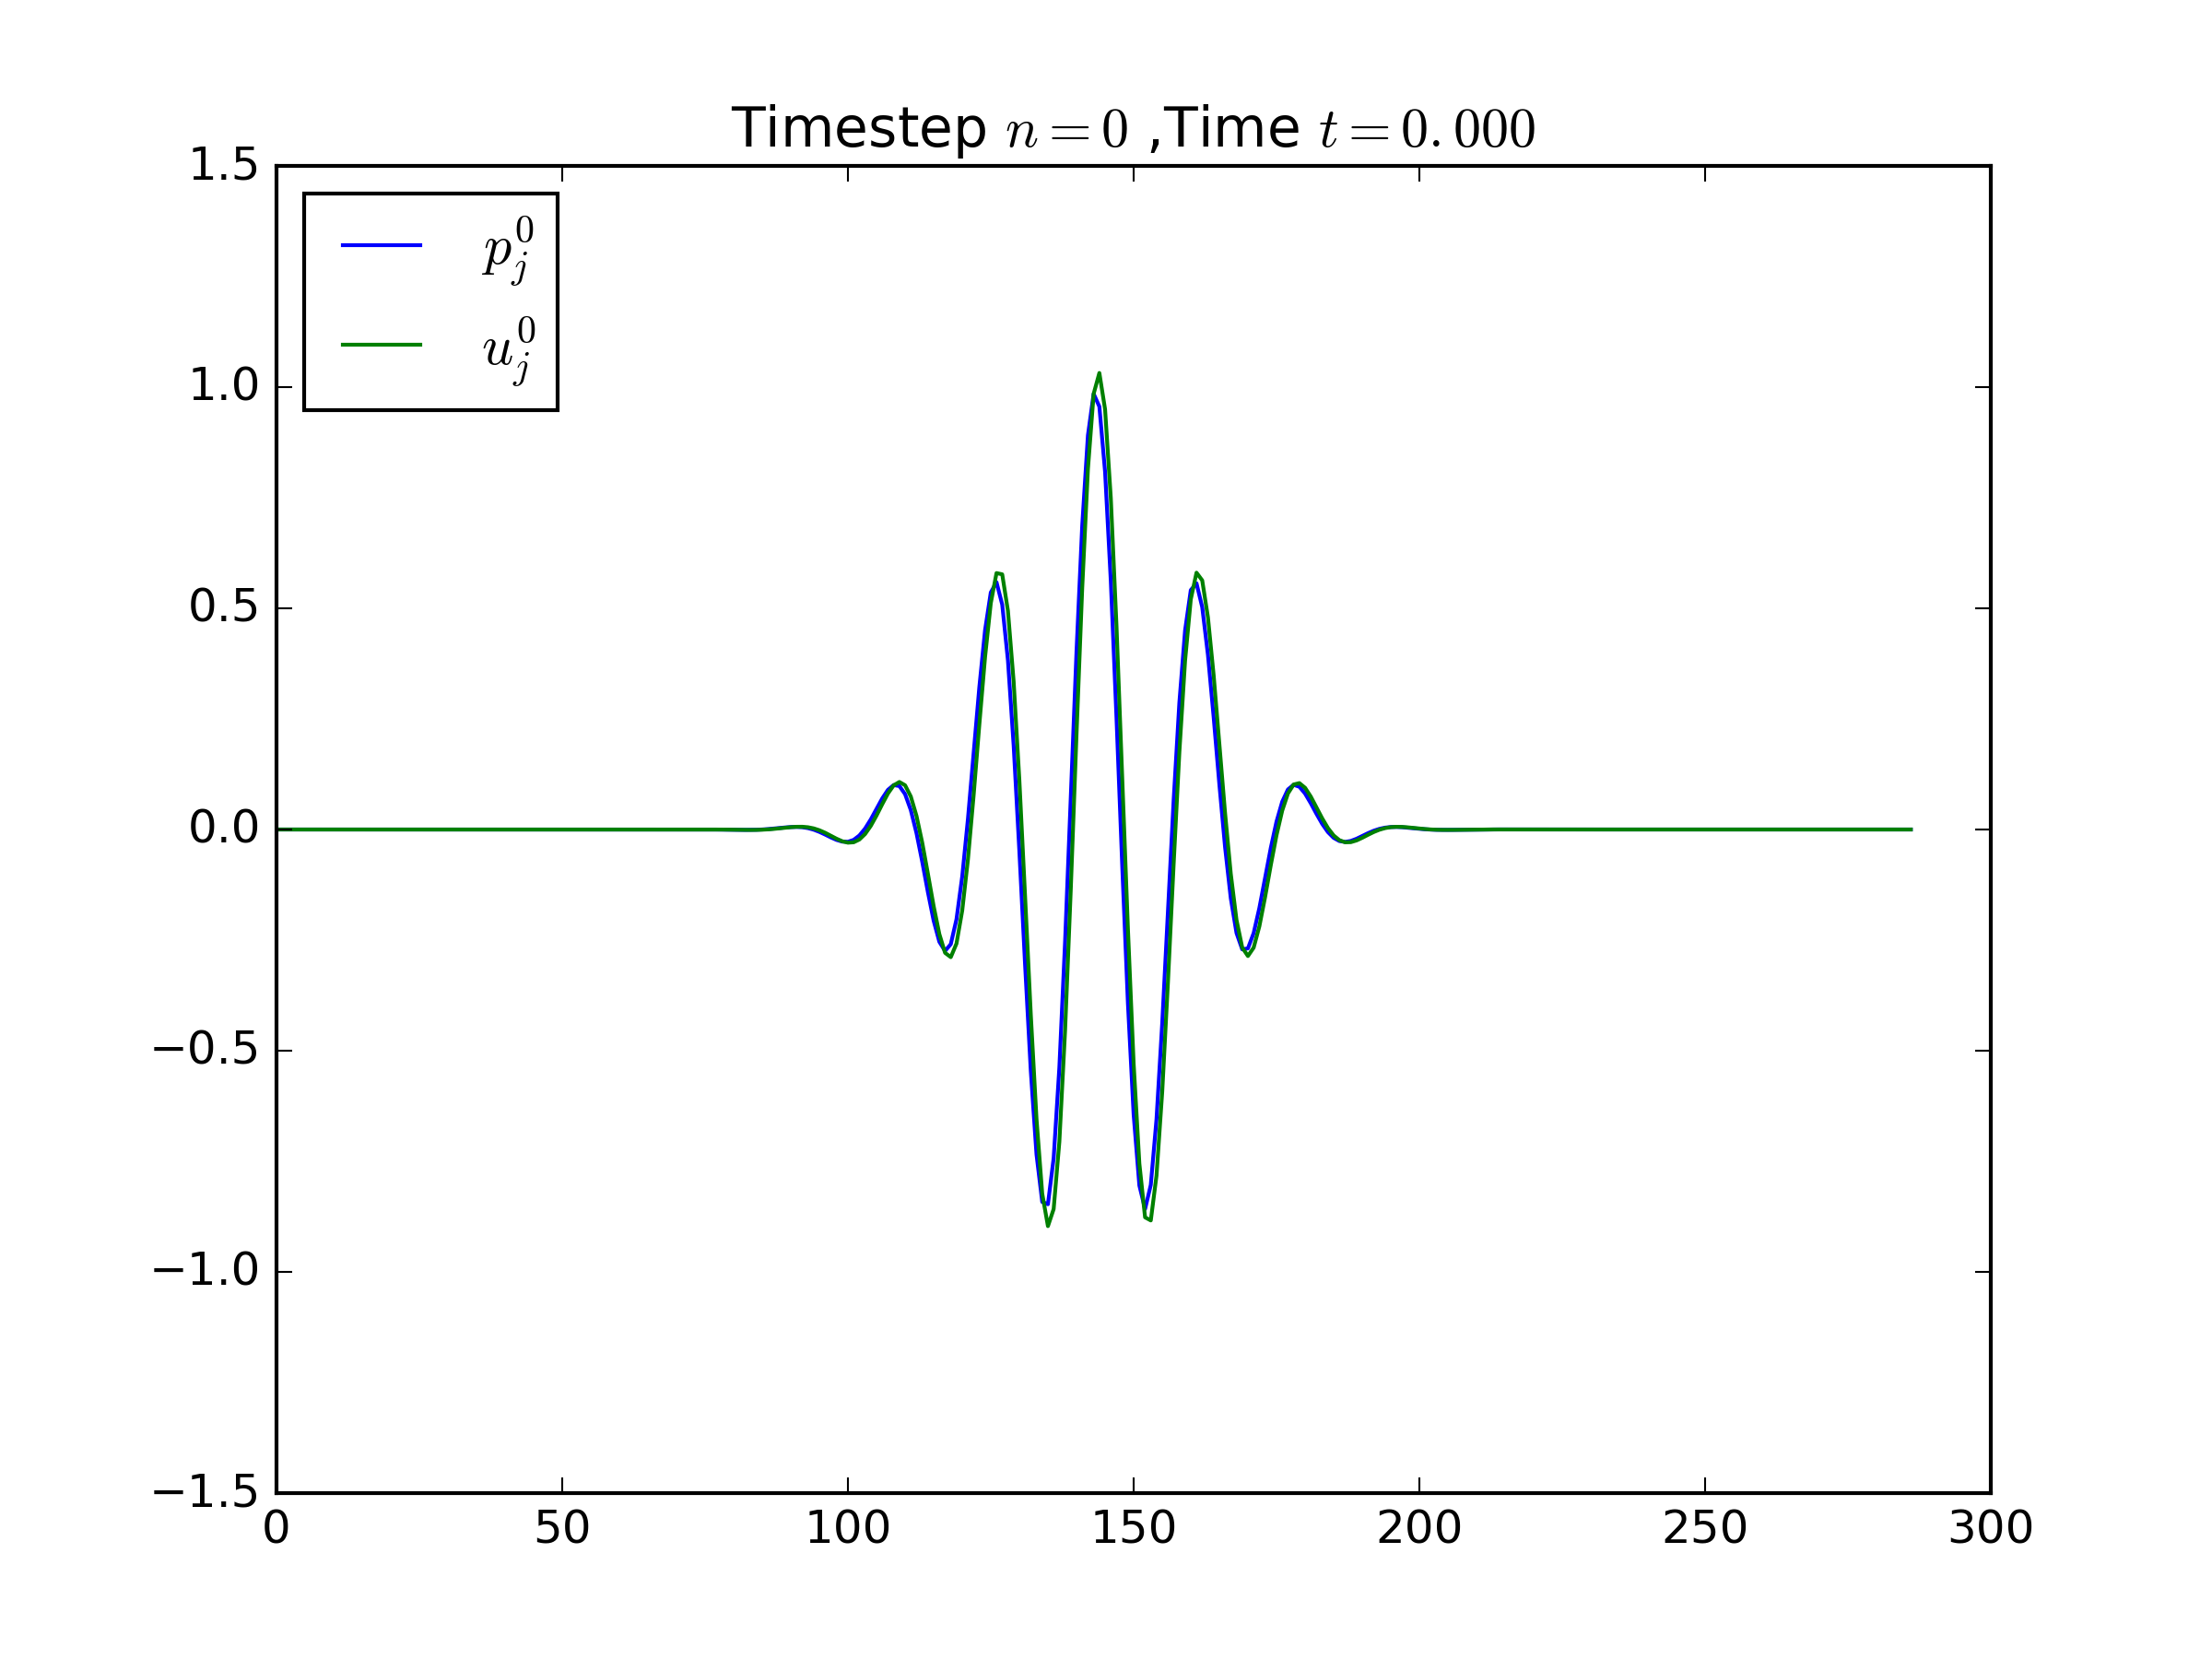
\includegraphics[width=0.31\textwidth]{figures/problem_1_a_000.png}
            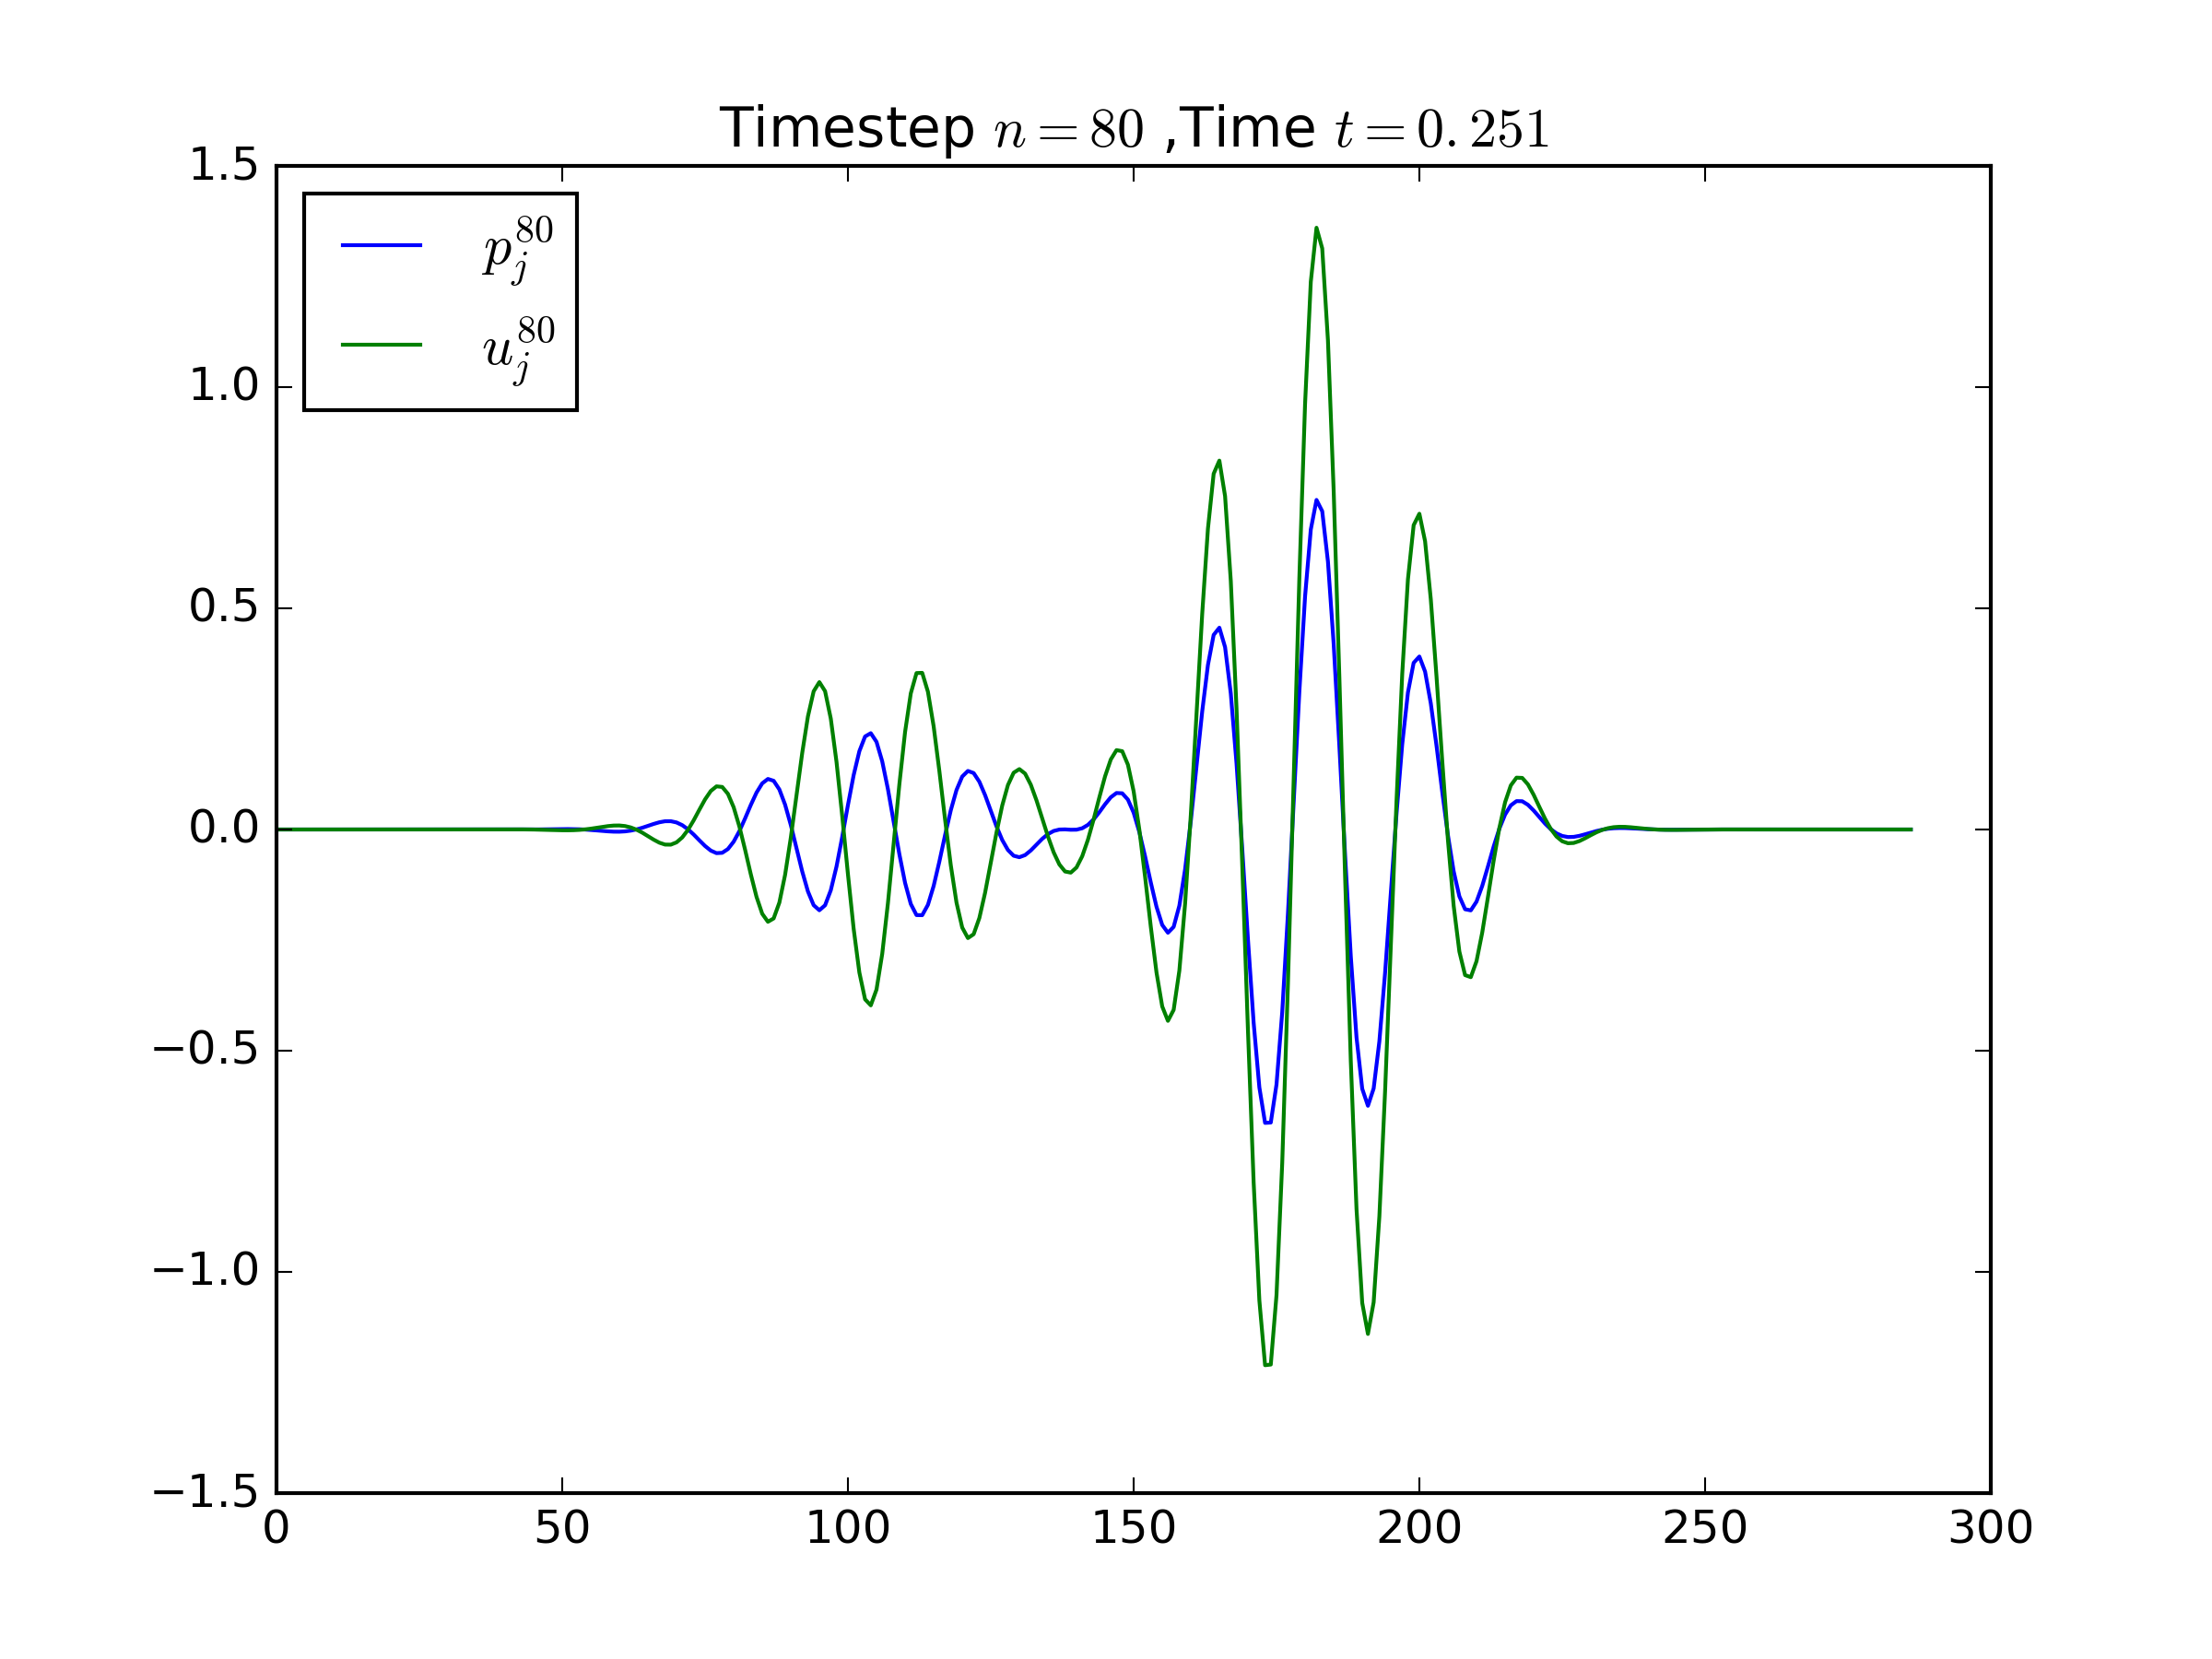
\includegraphics[width=0.31\textwidth]{figures/problem_1_a_008.png}
            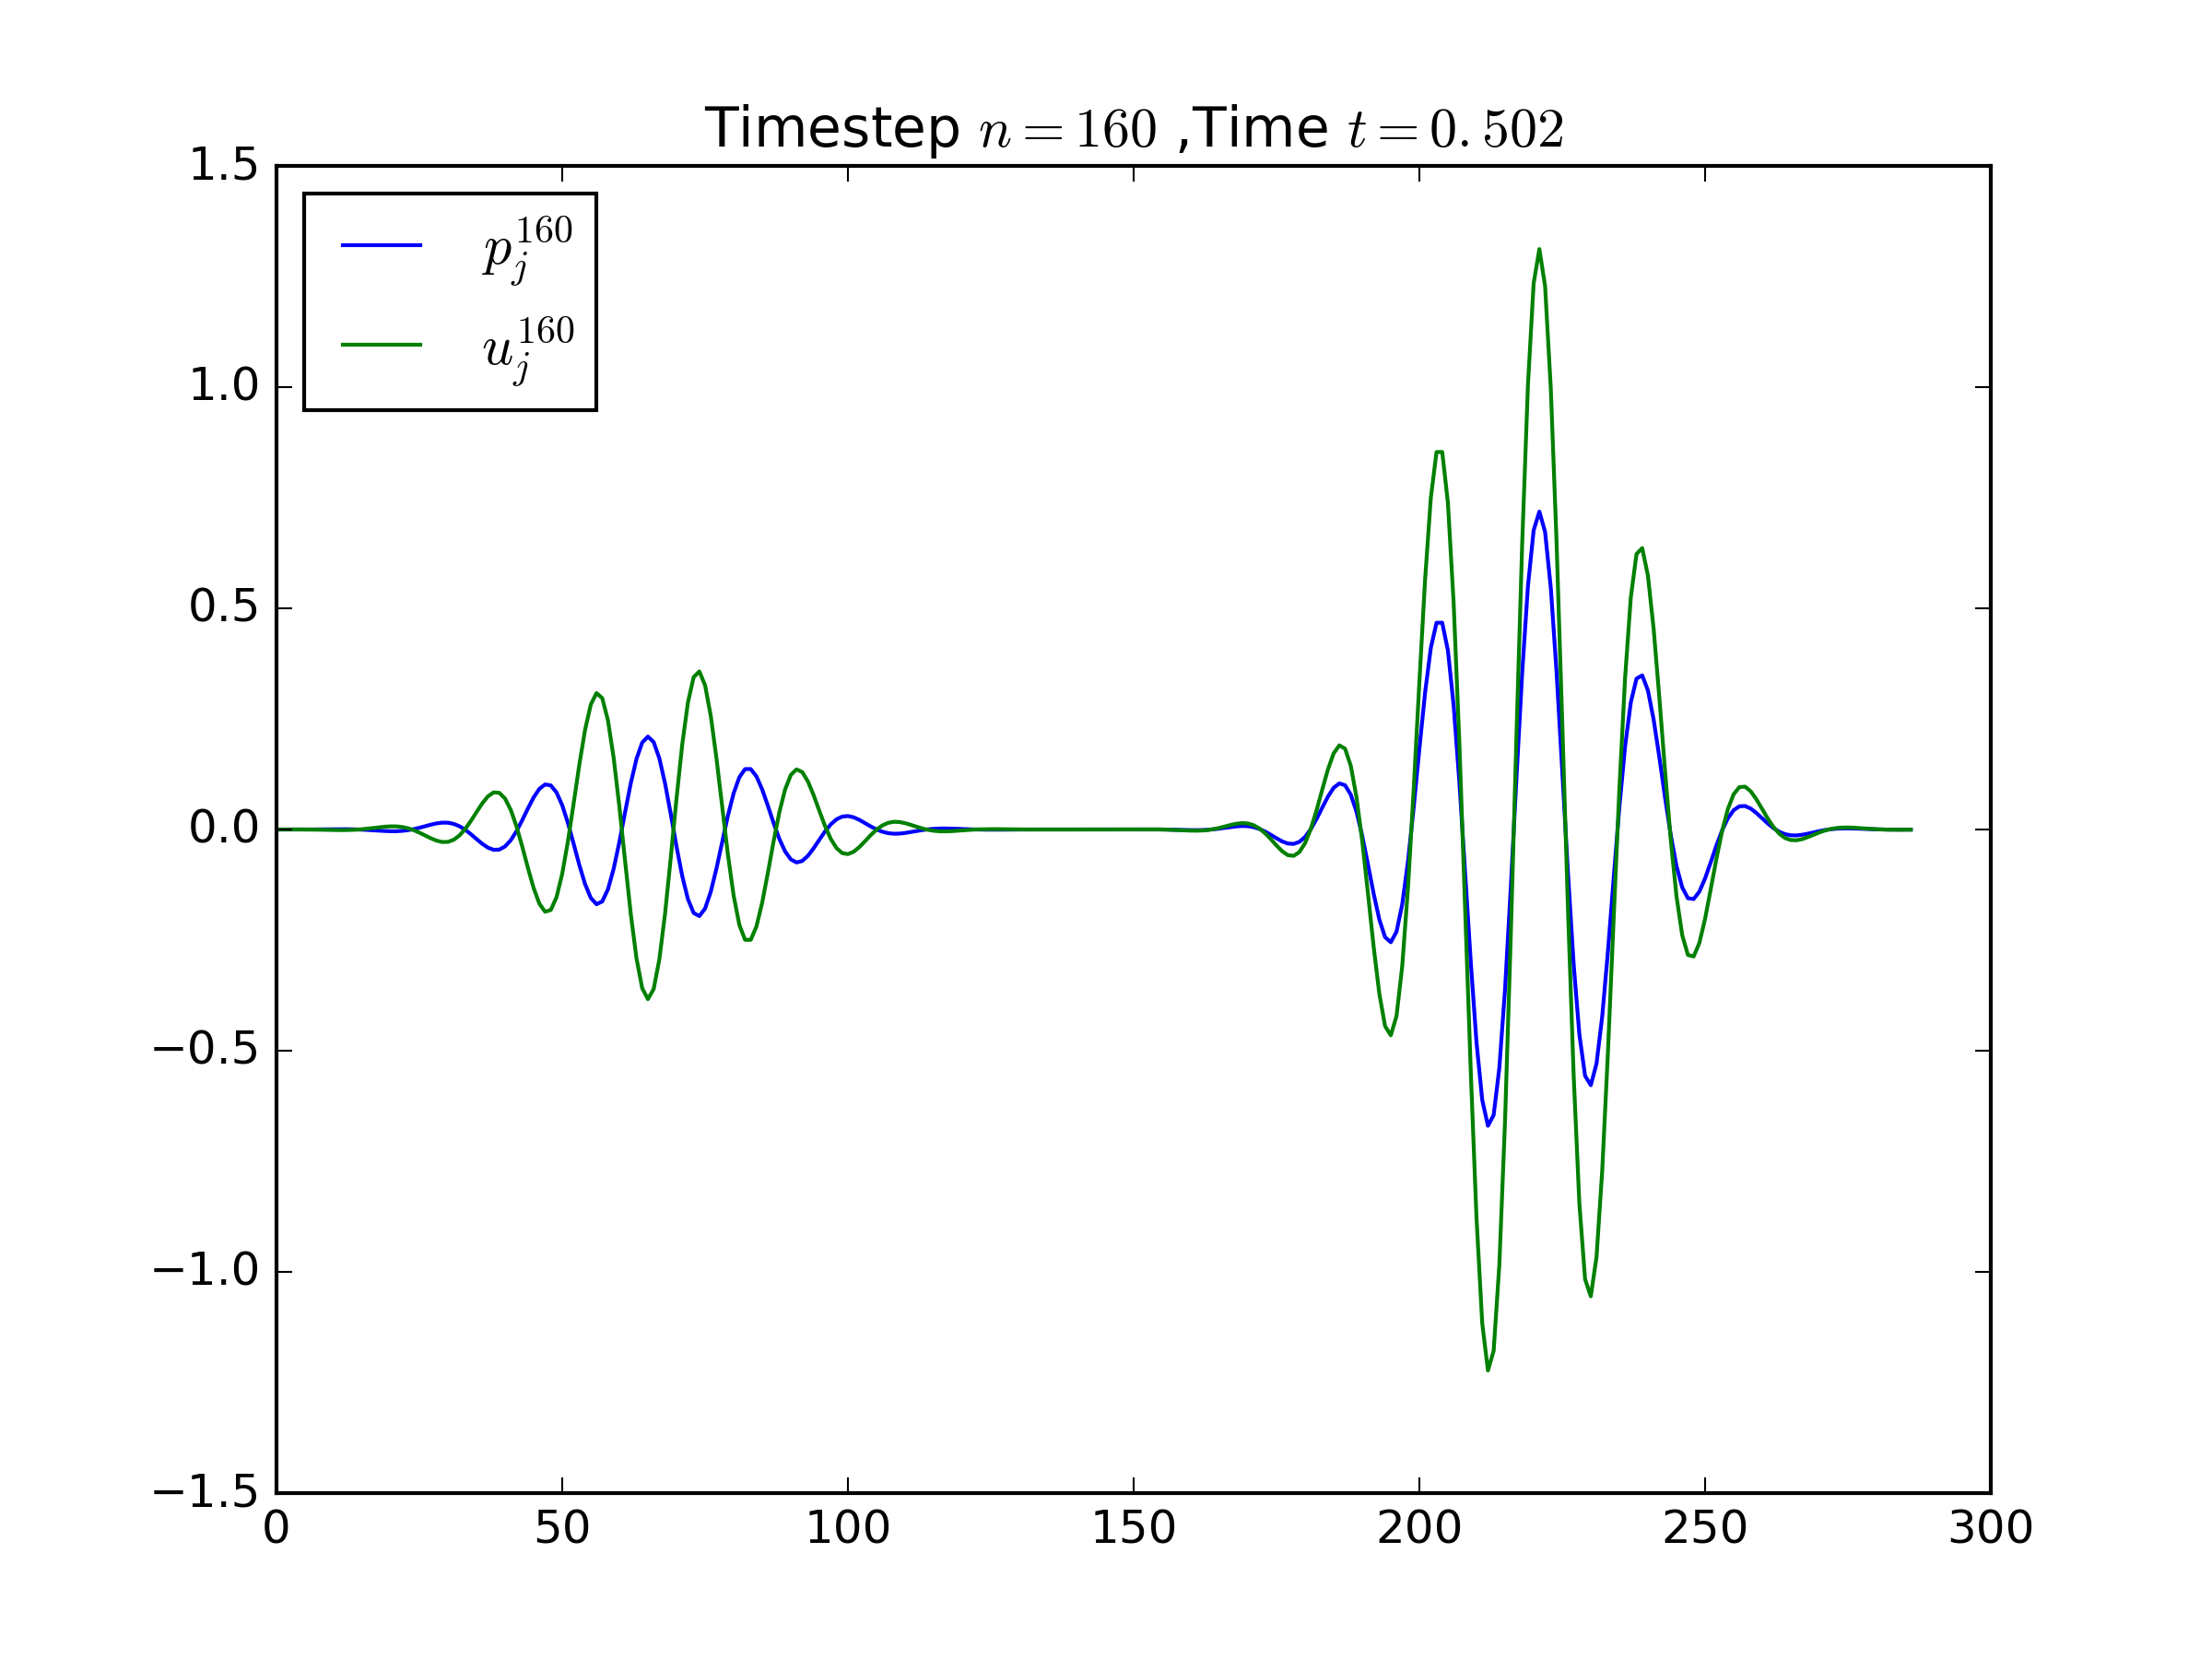
\includegraphics[width=0.31\textwidth]{figures/problem_1_a_016.png}
            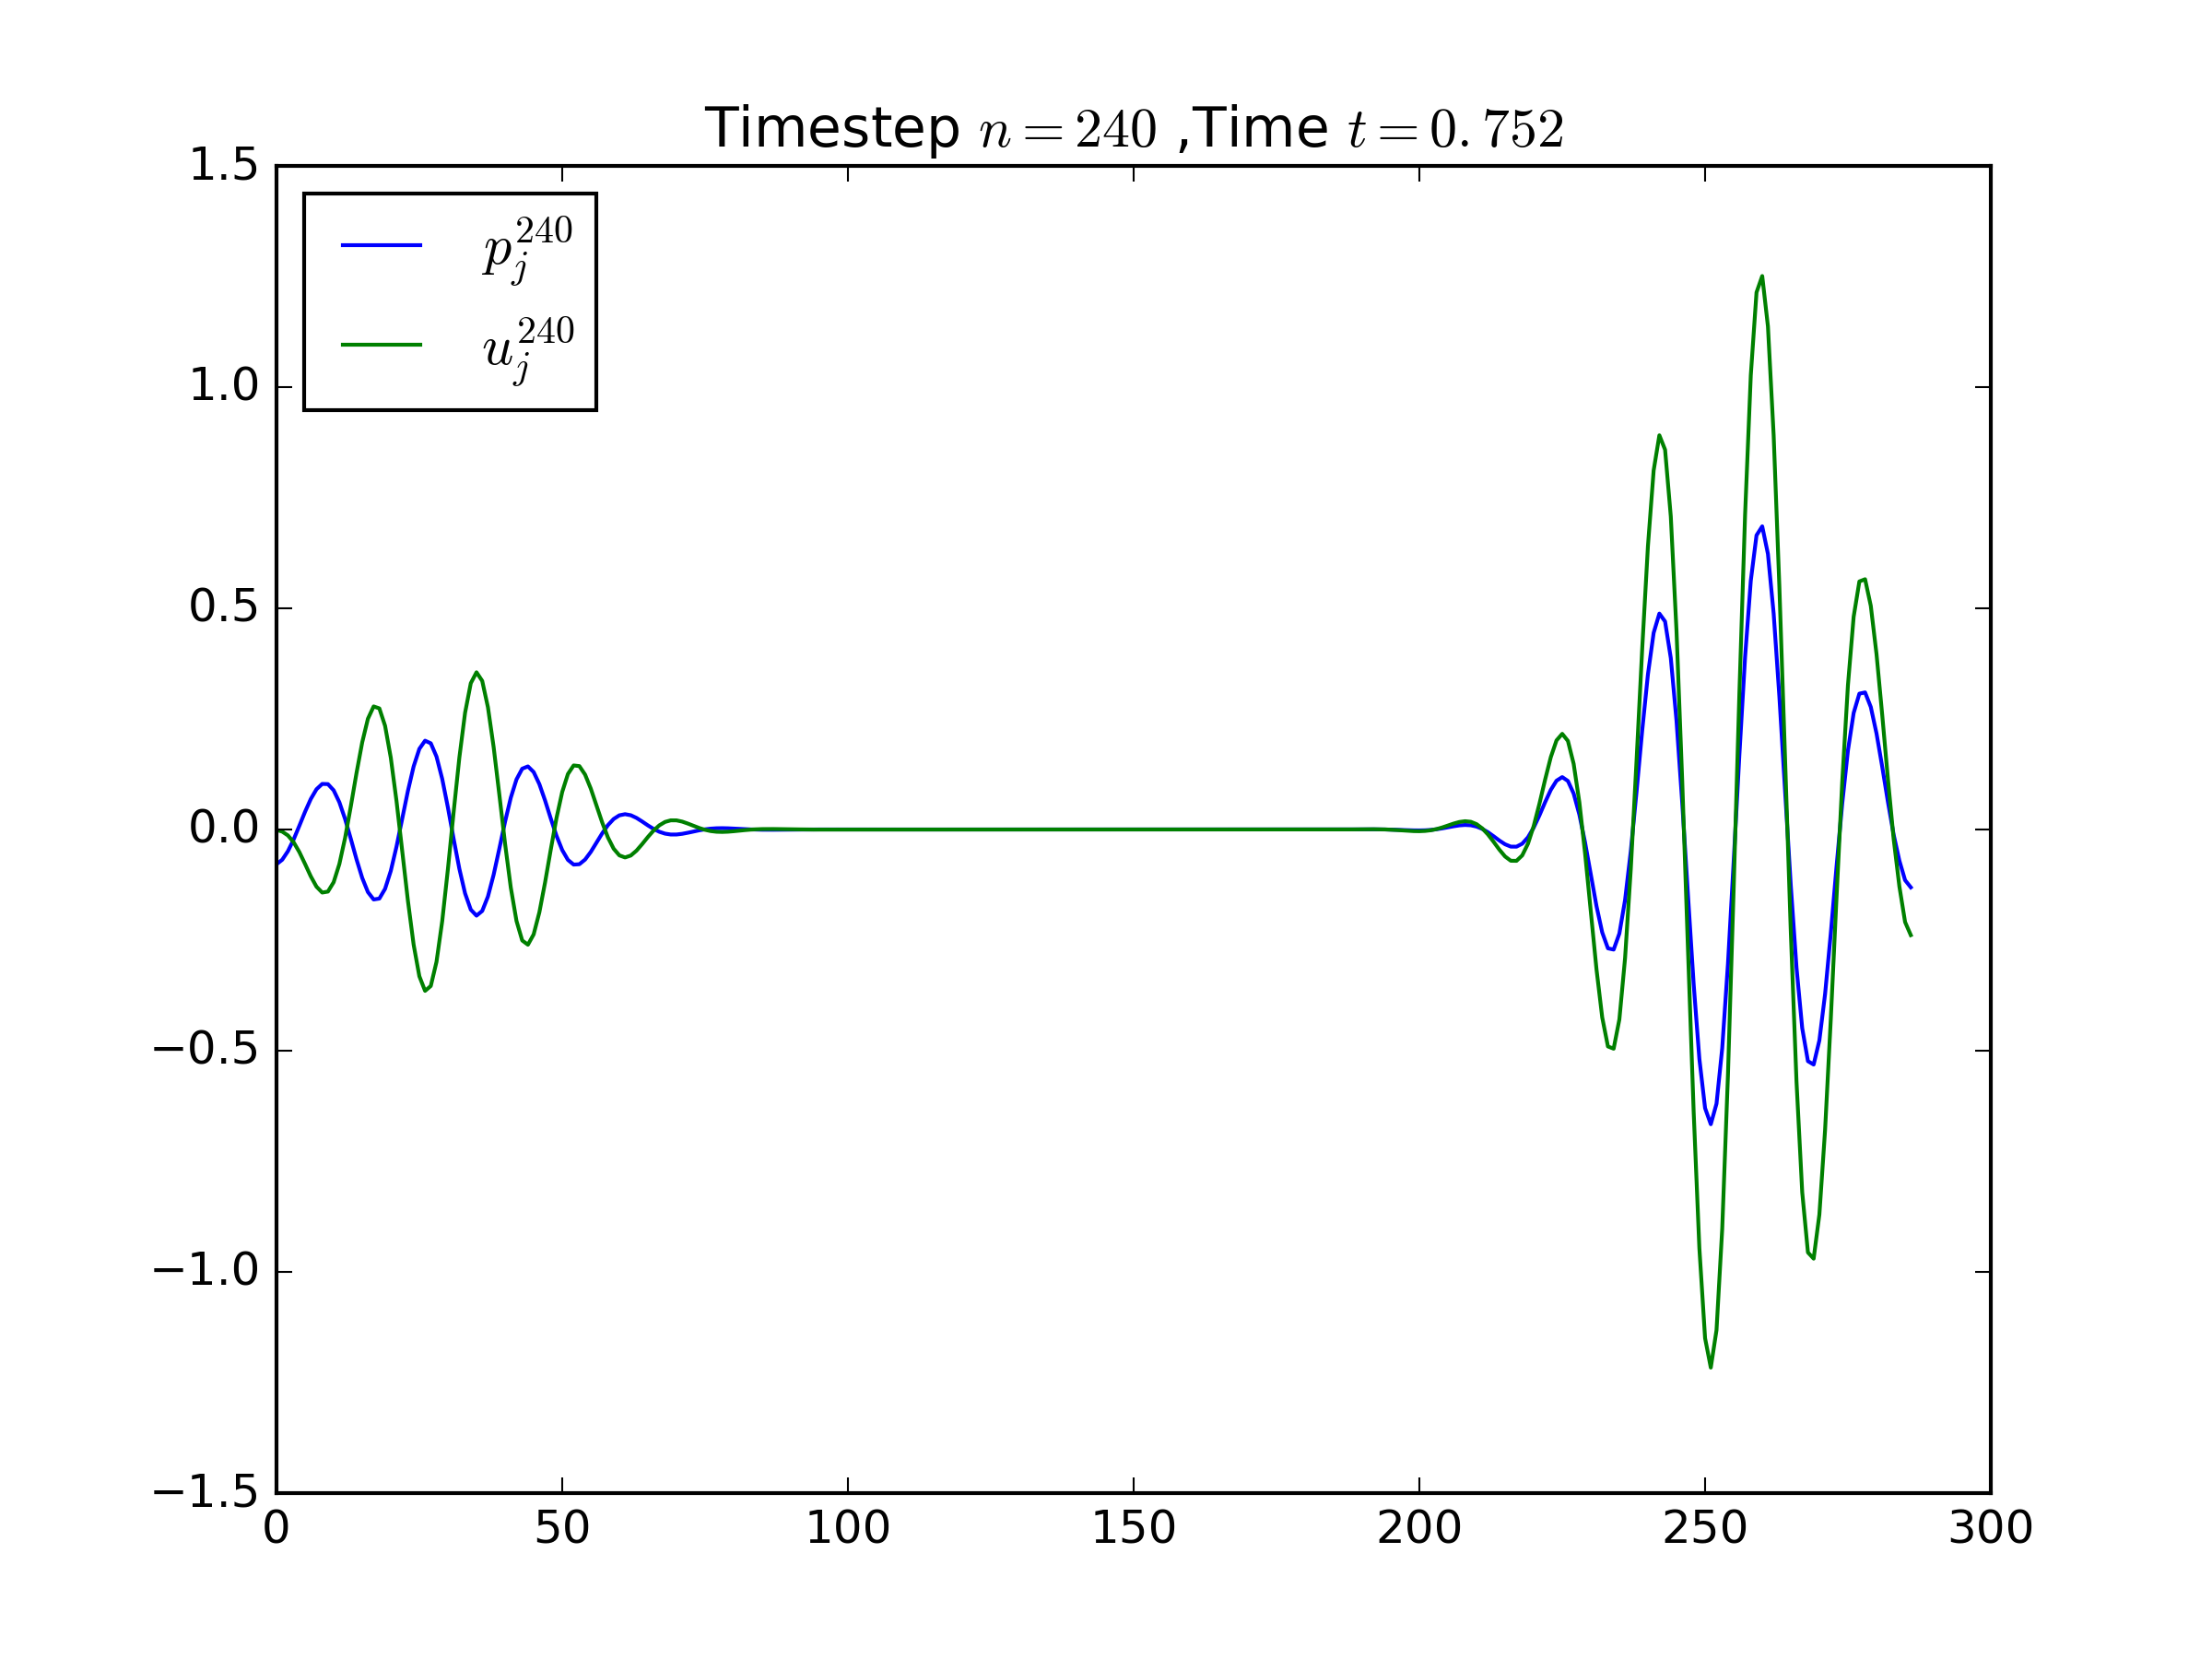
\includegraphics[width=0.31\textwidth]{figures/problem_1_a_024.png}
            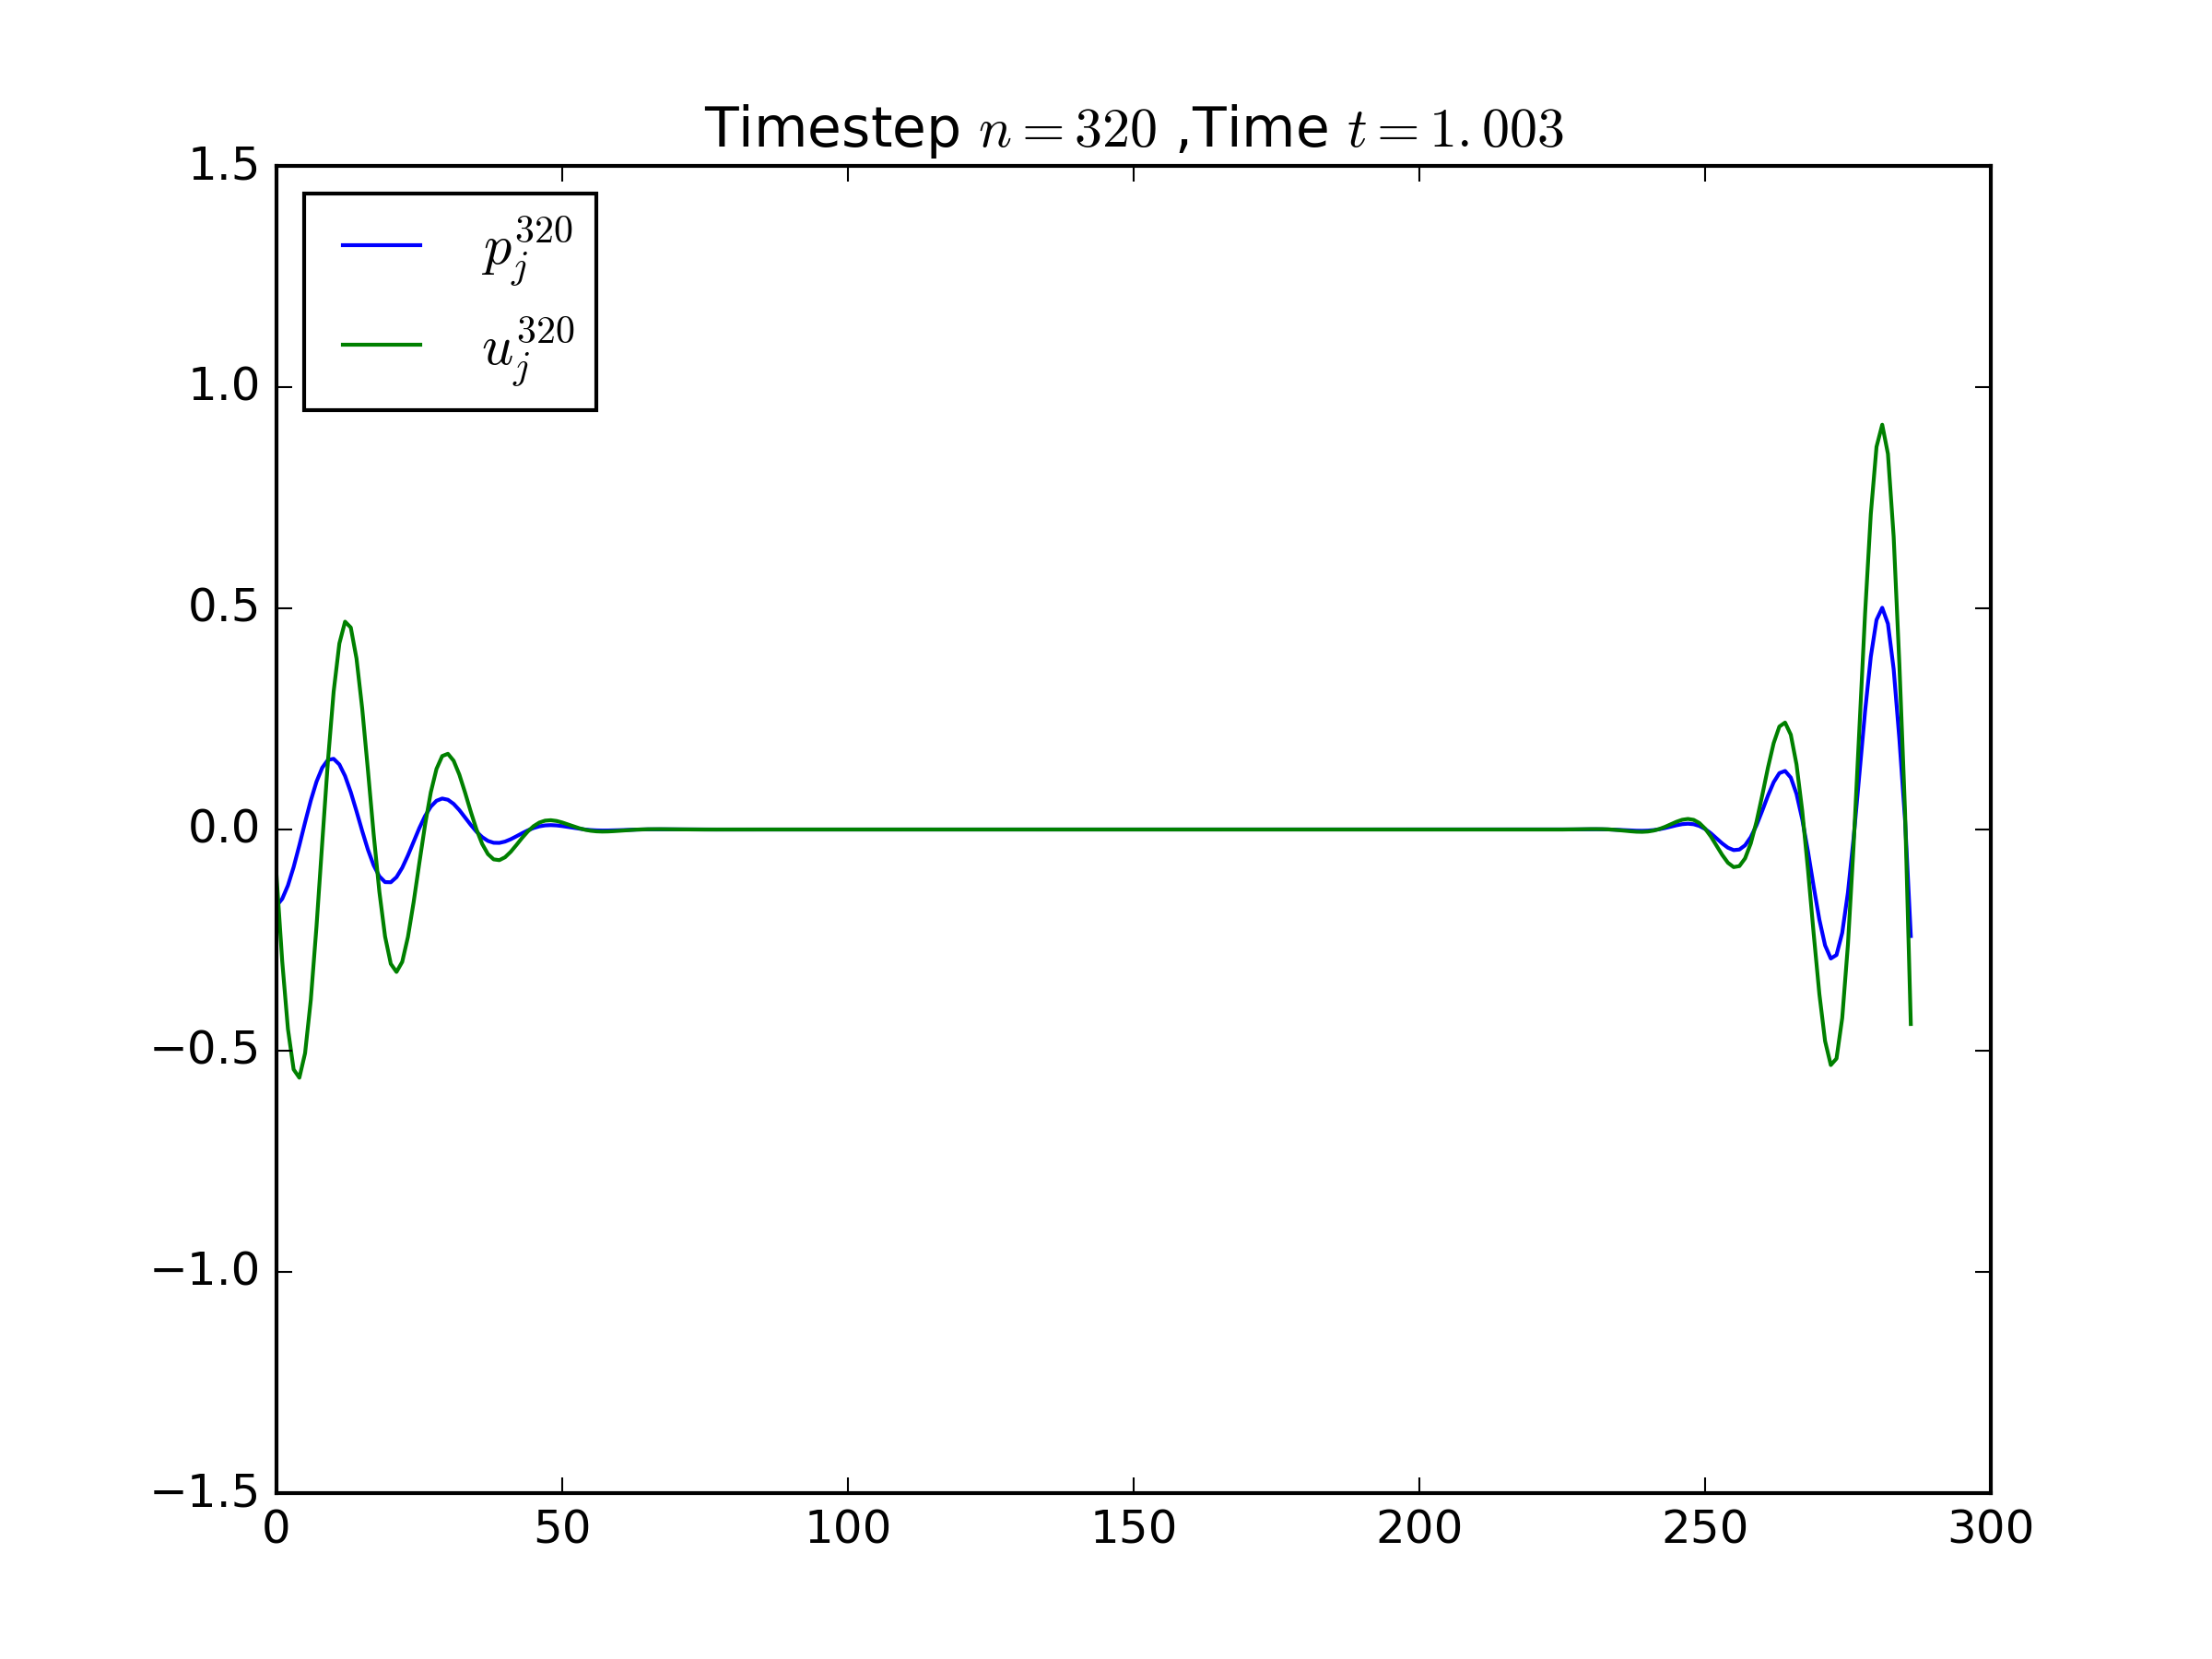
\includegraphics[width=0.31\textwidth]{figures/problem_1_a_032.png}
            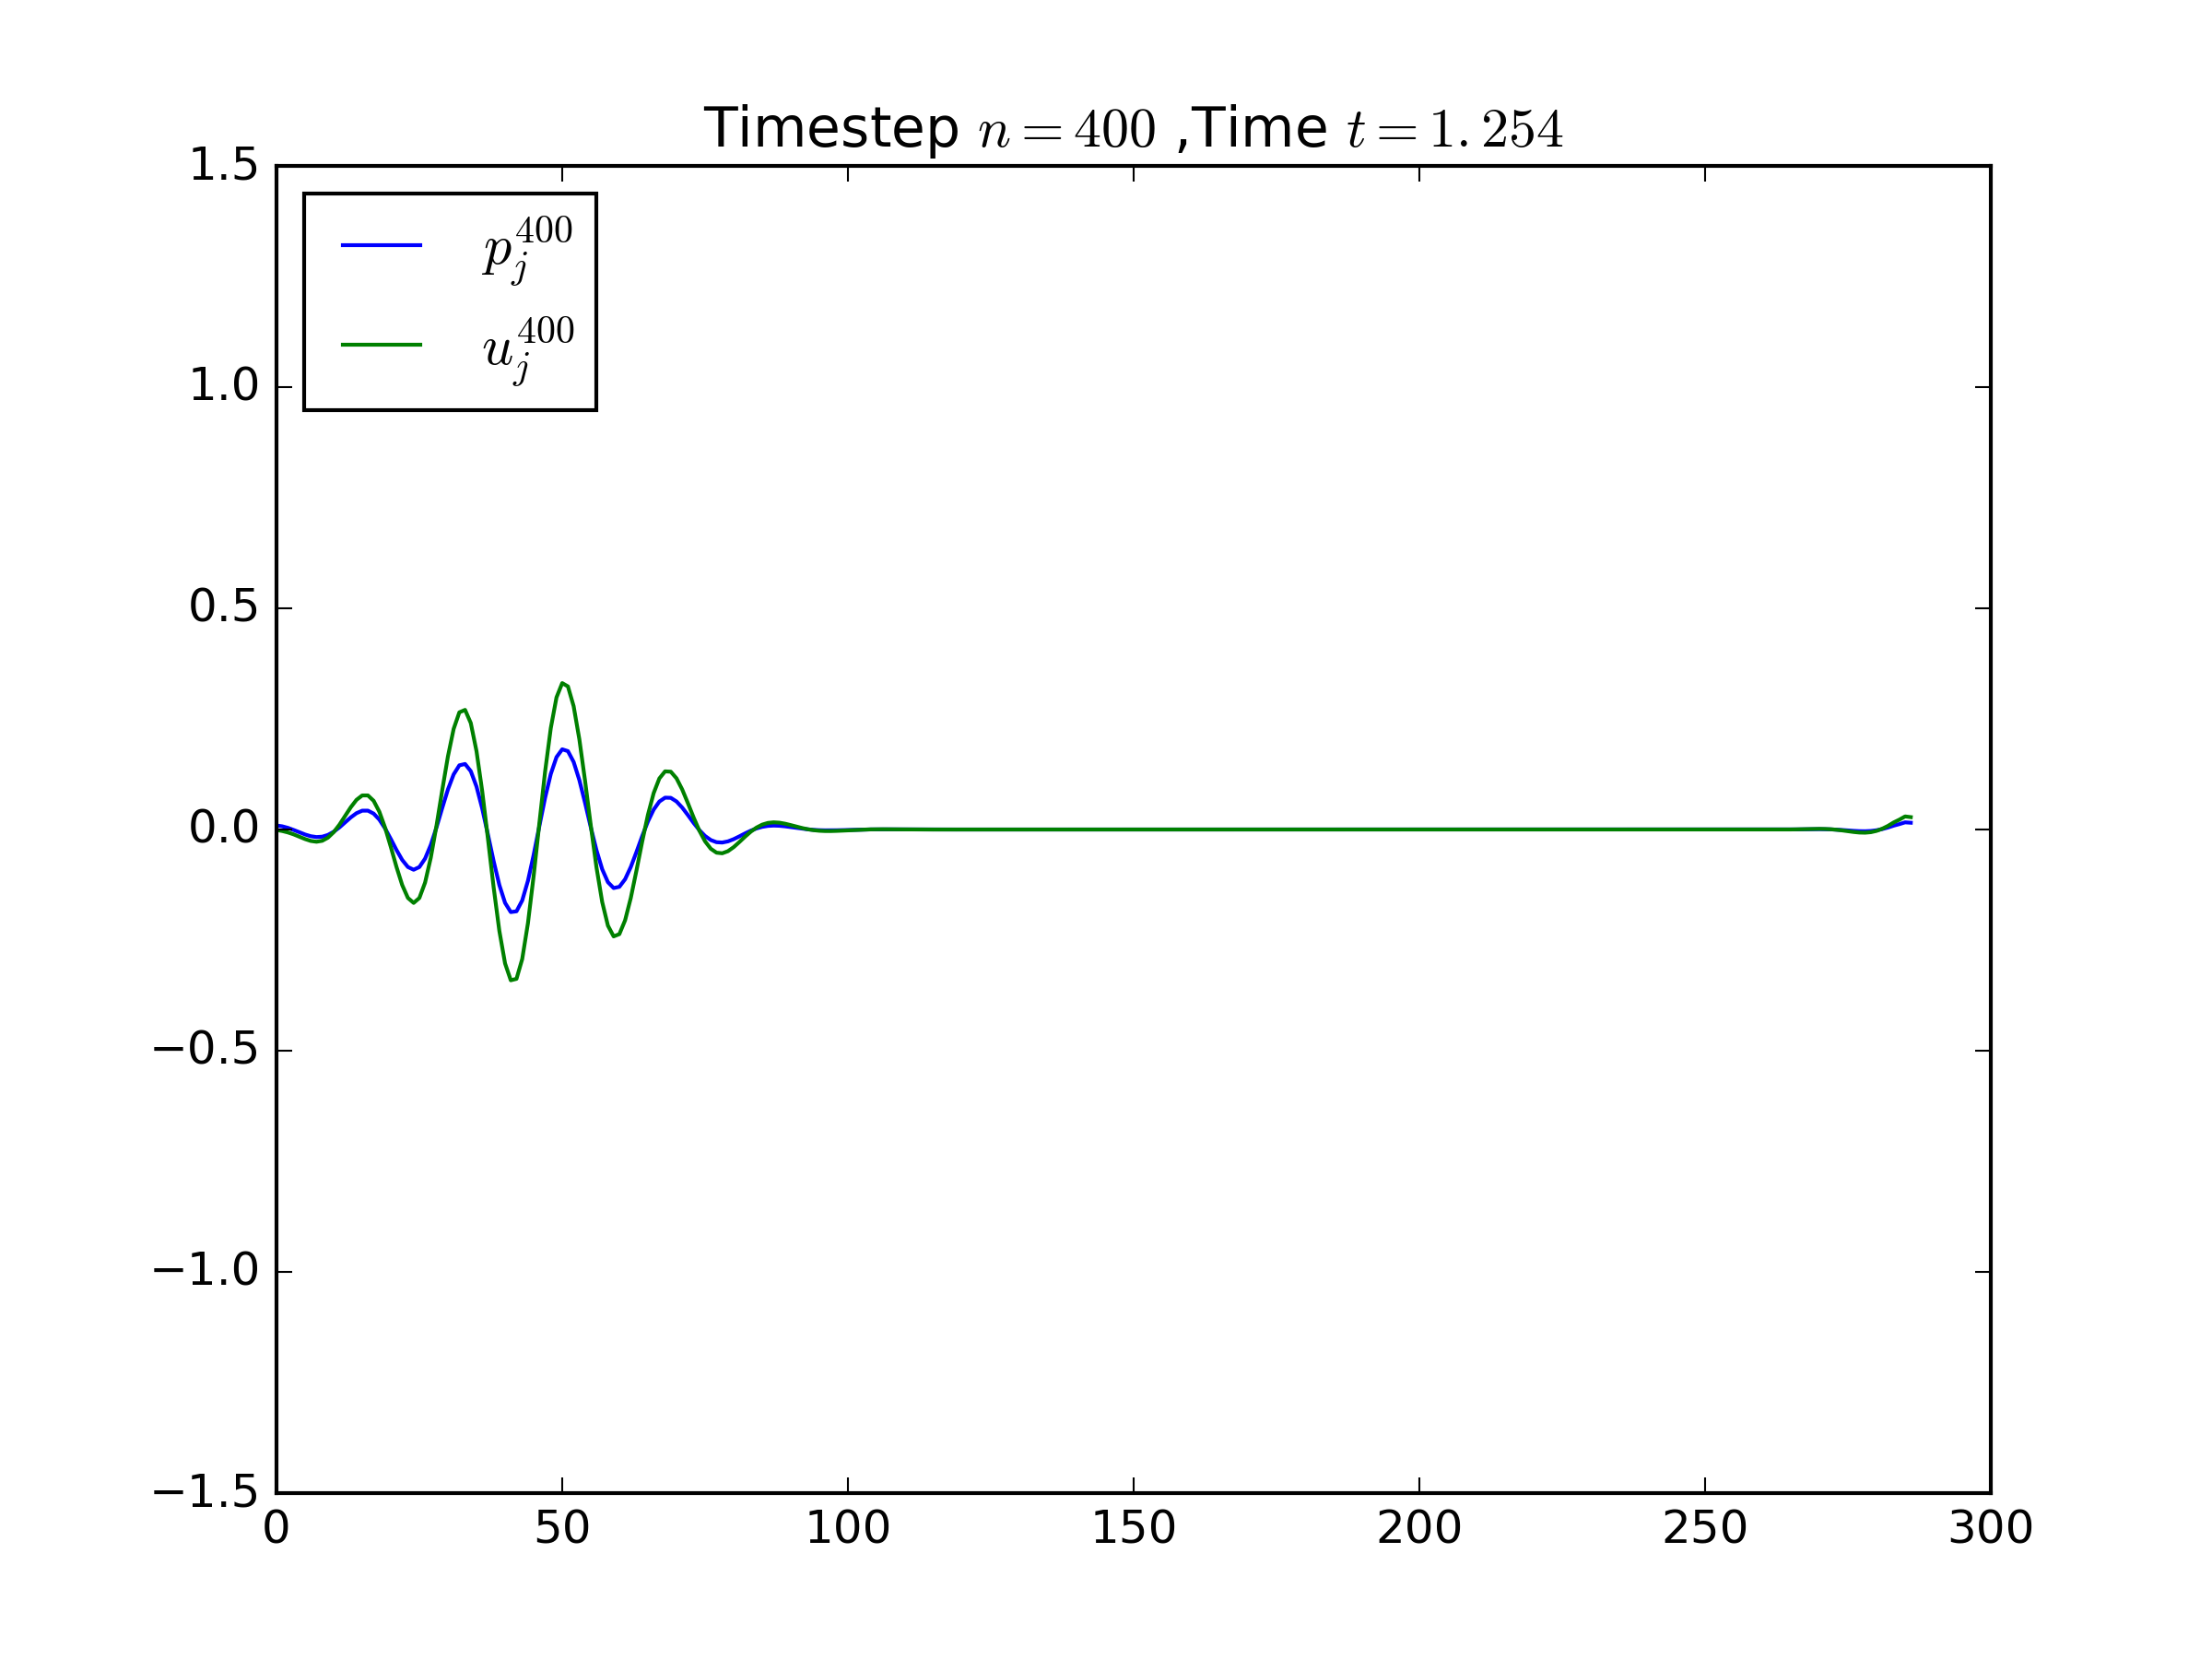
\includegraphics[width=0.31\textwidth]{figures/problem_1_a_040.png}
            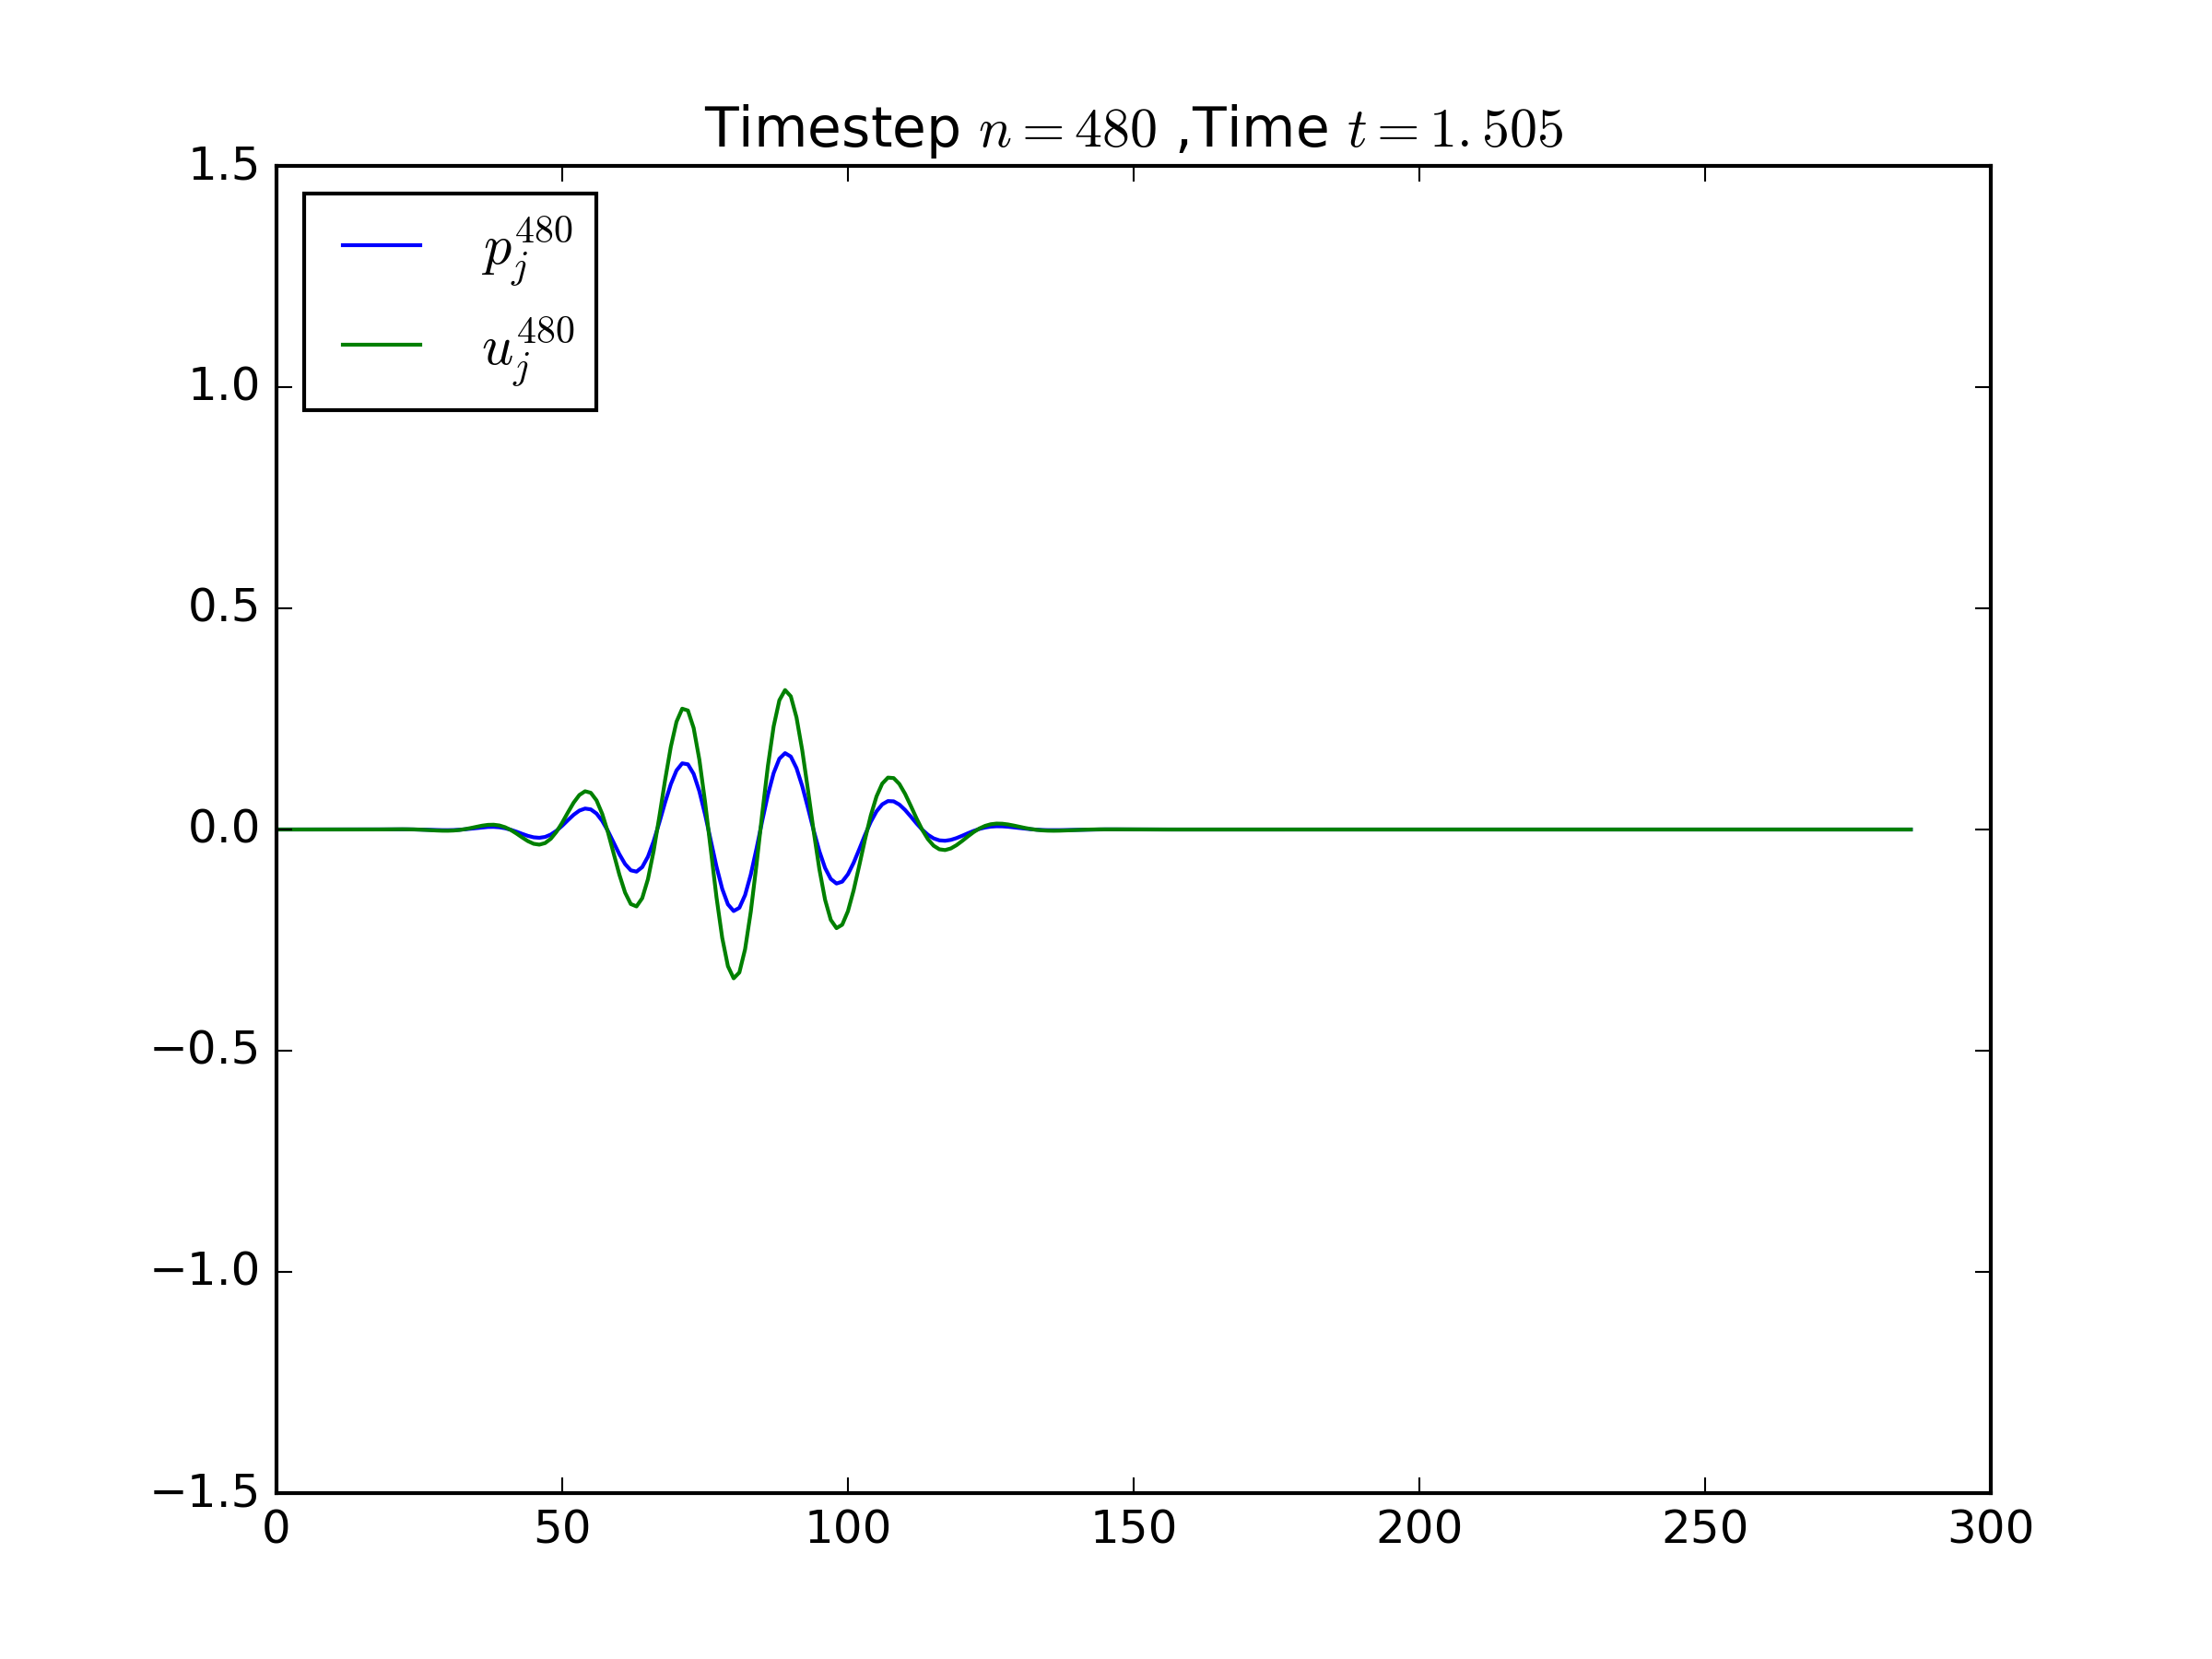
\includegraphics[width=0.31\textwidth]{figures/problem_1_a_048.png}
            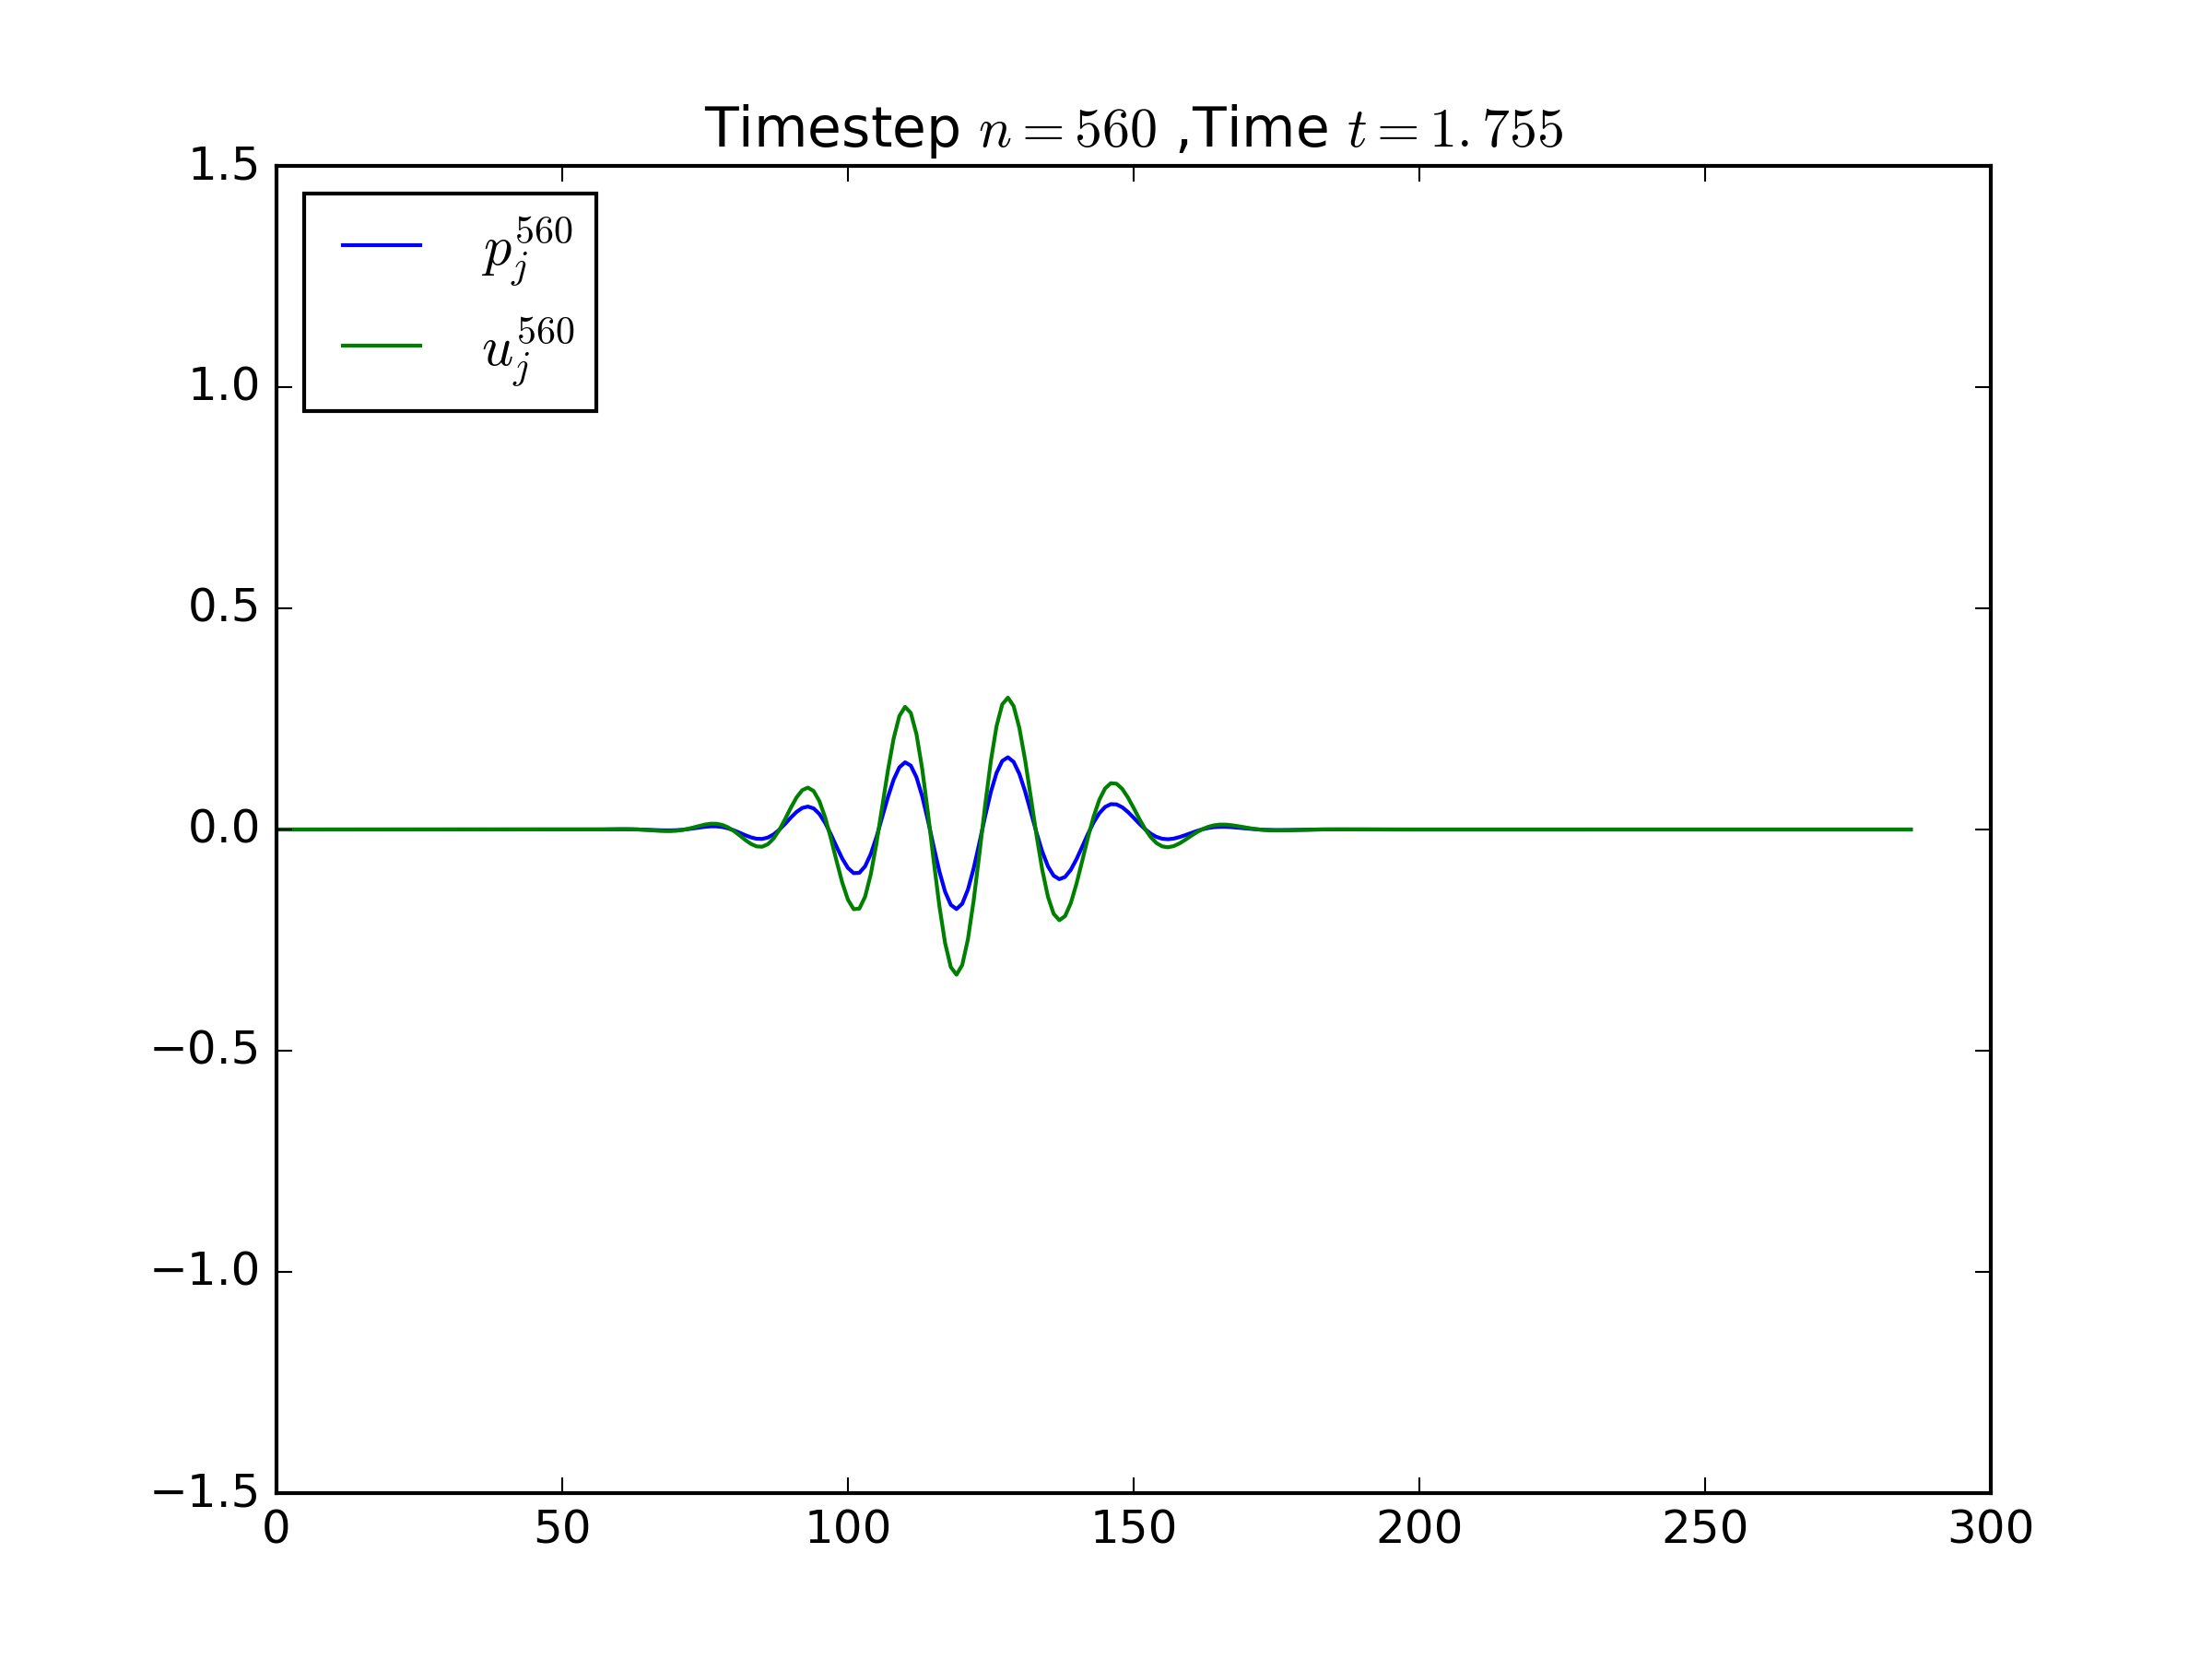
\includegraphics[width=0.31\textwidth]{figures/problem_1_a_056.png}
            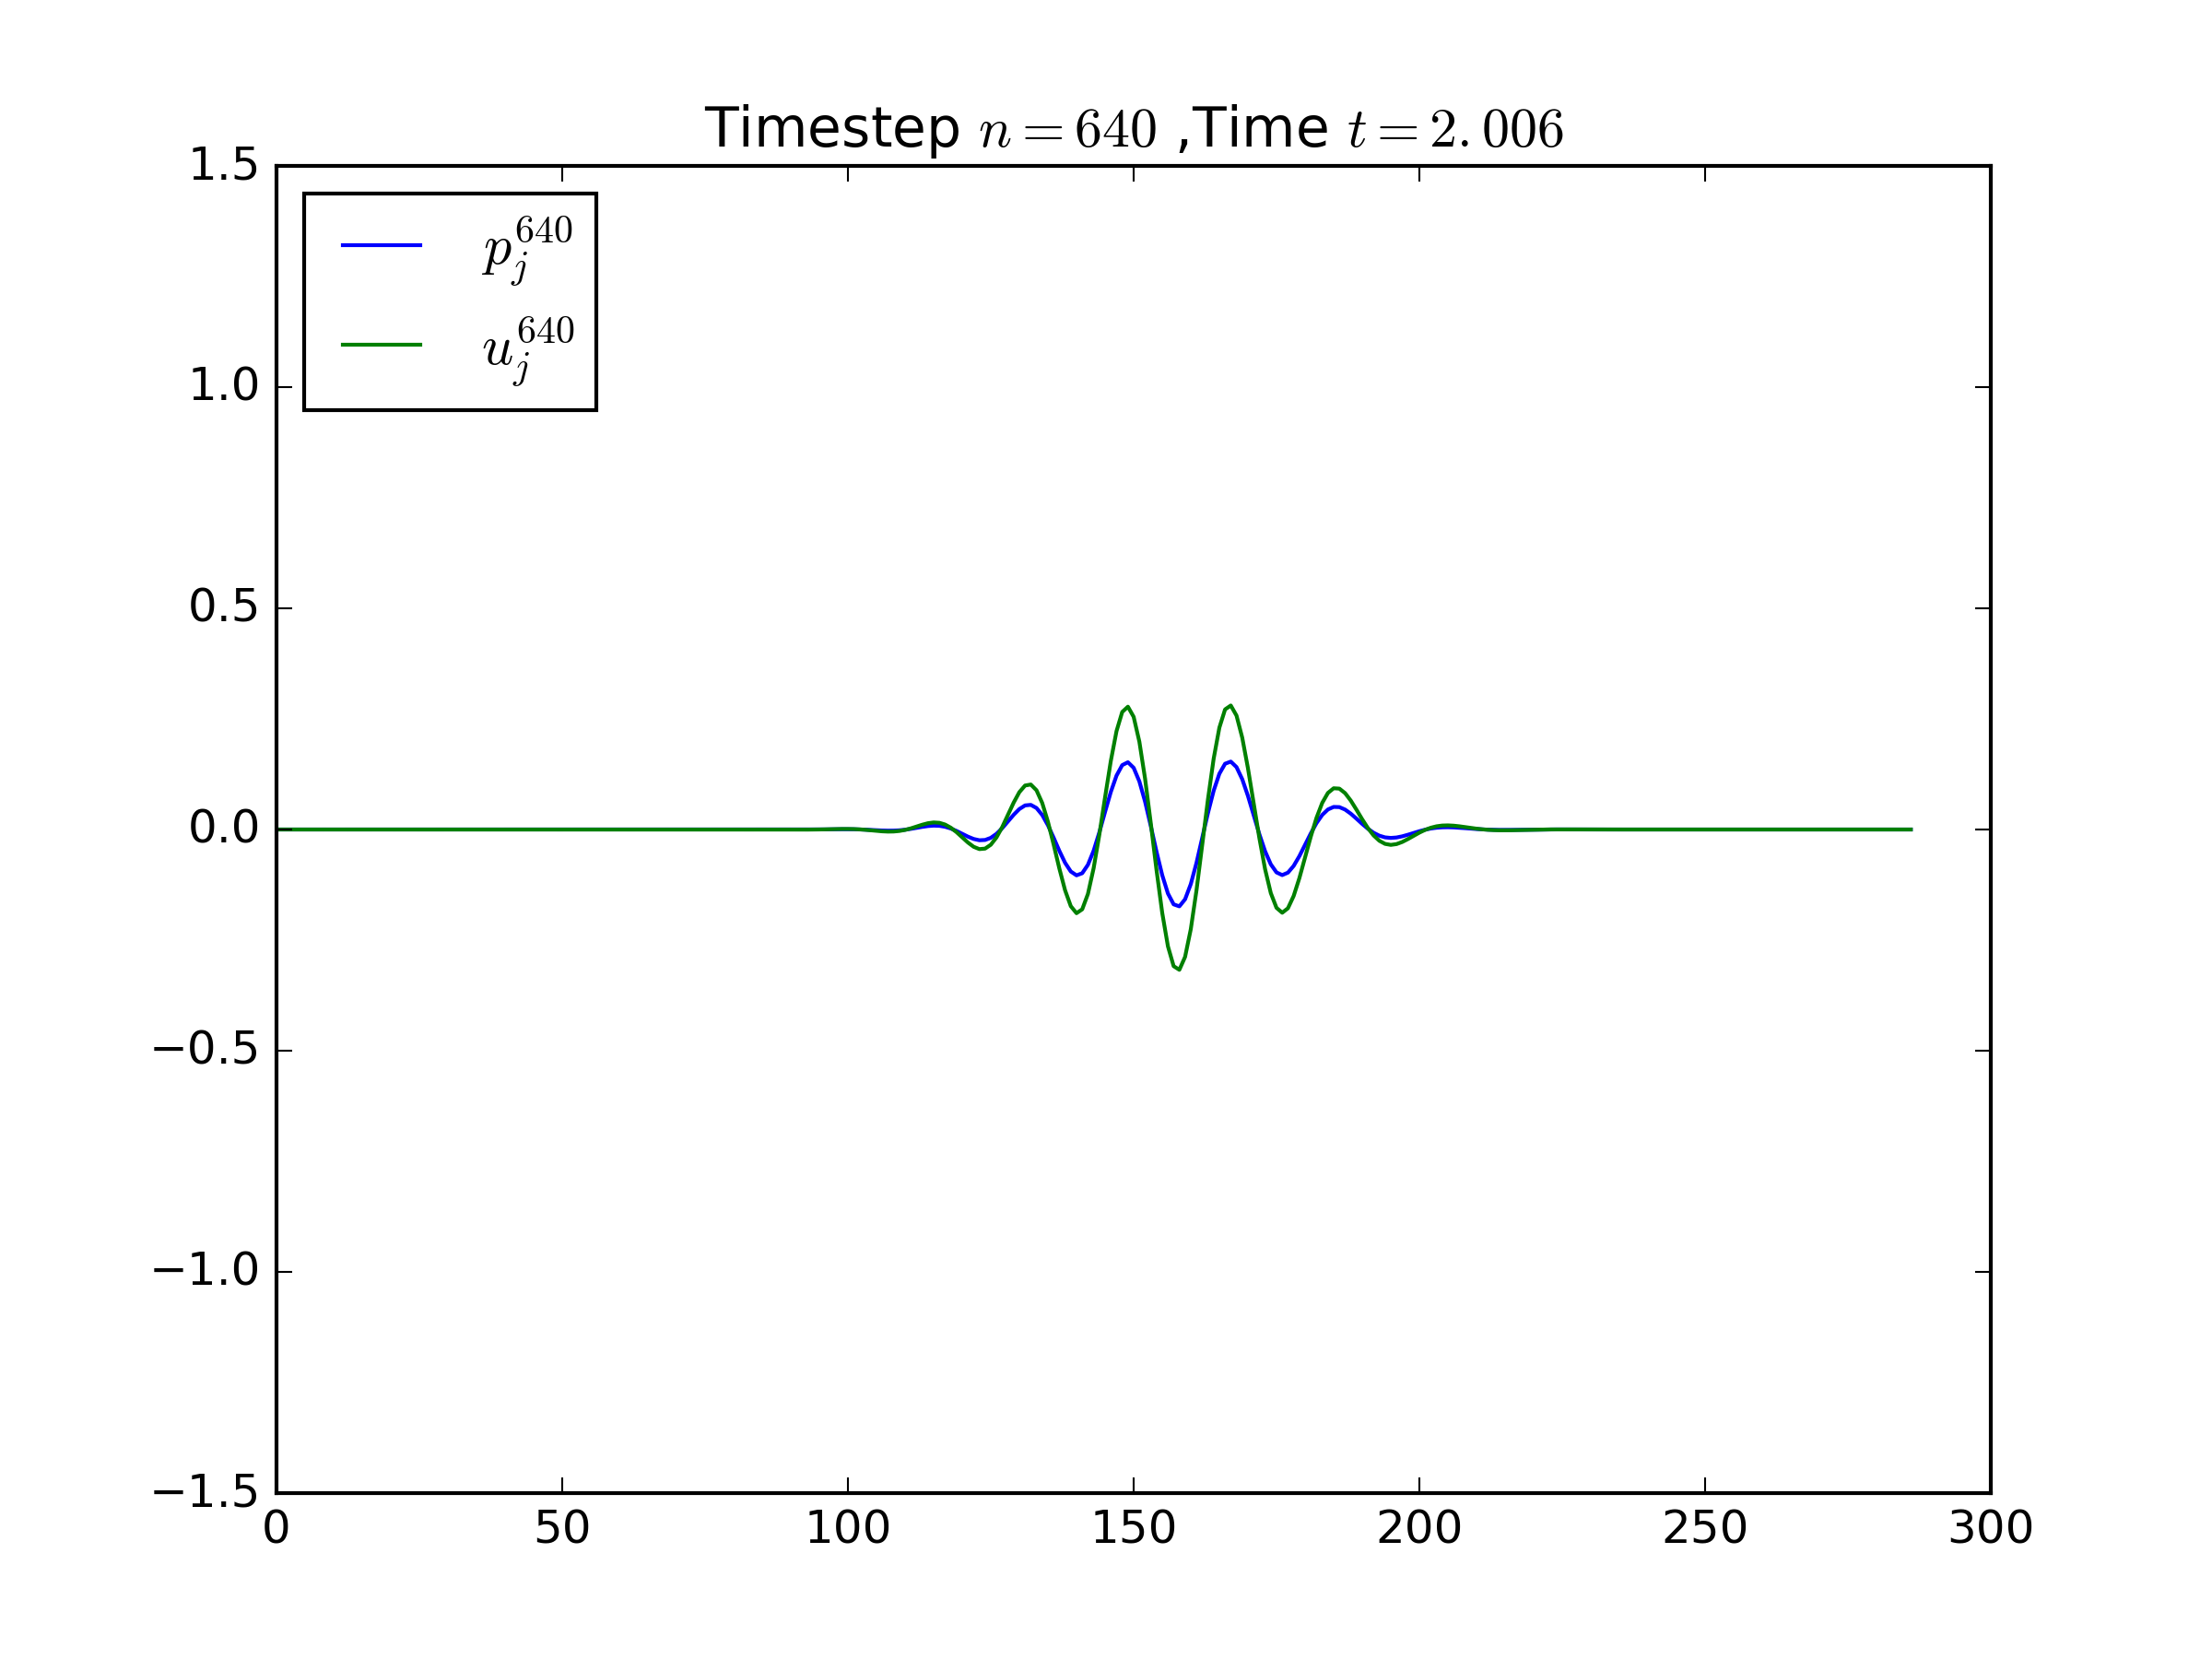
\includegraphics[width=0.31\textwidth]{figures/problem_1_a_064.png}
            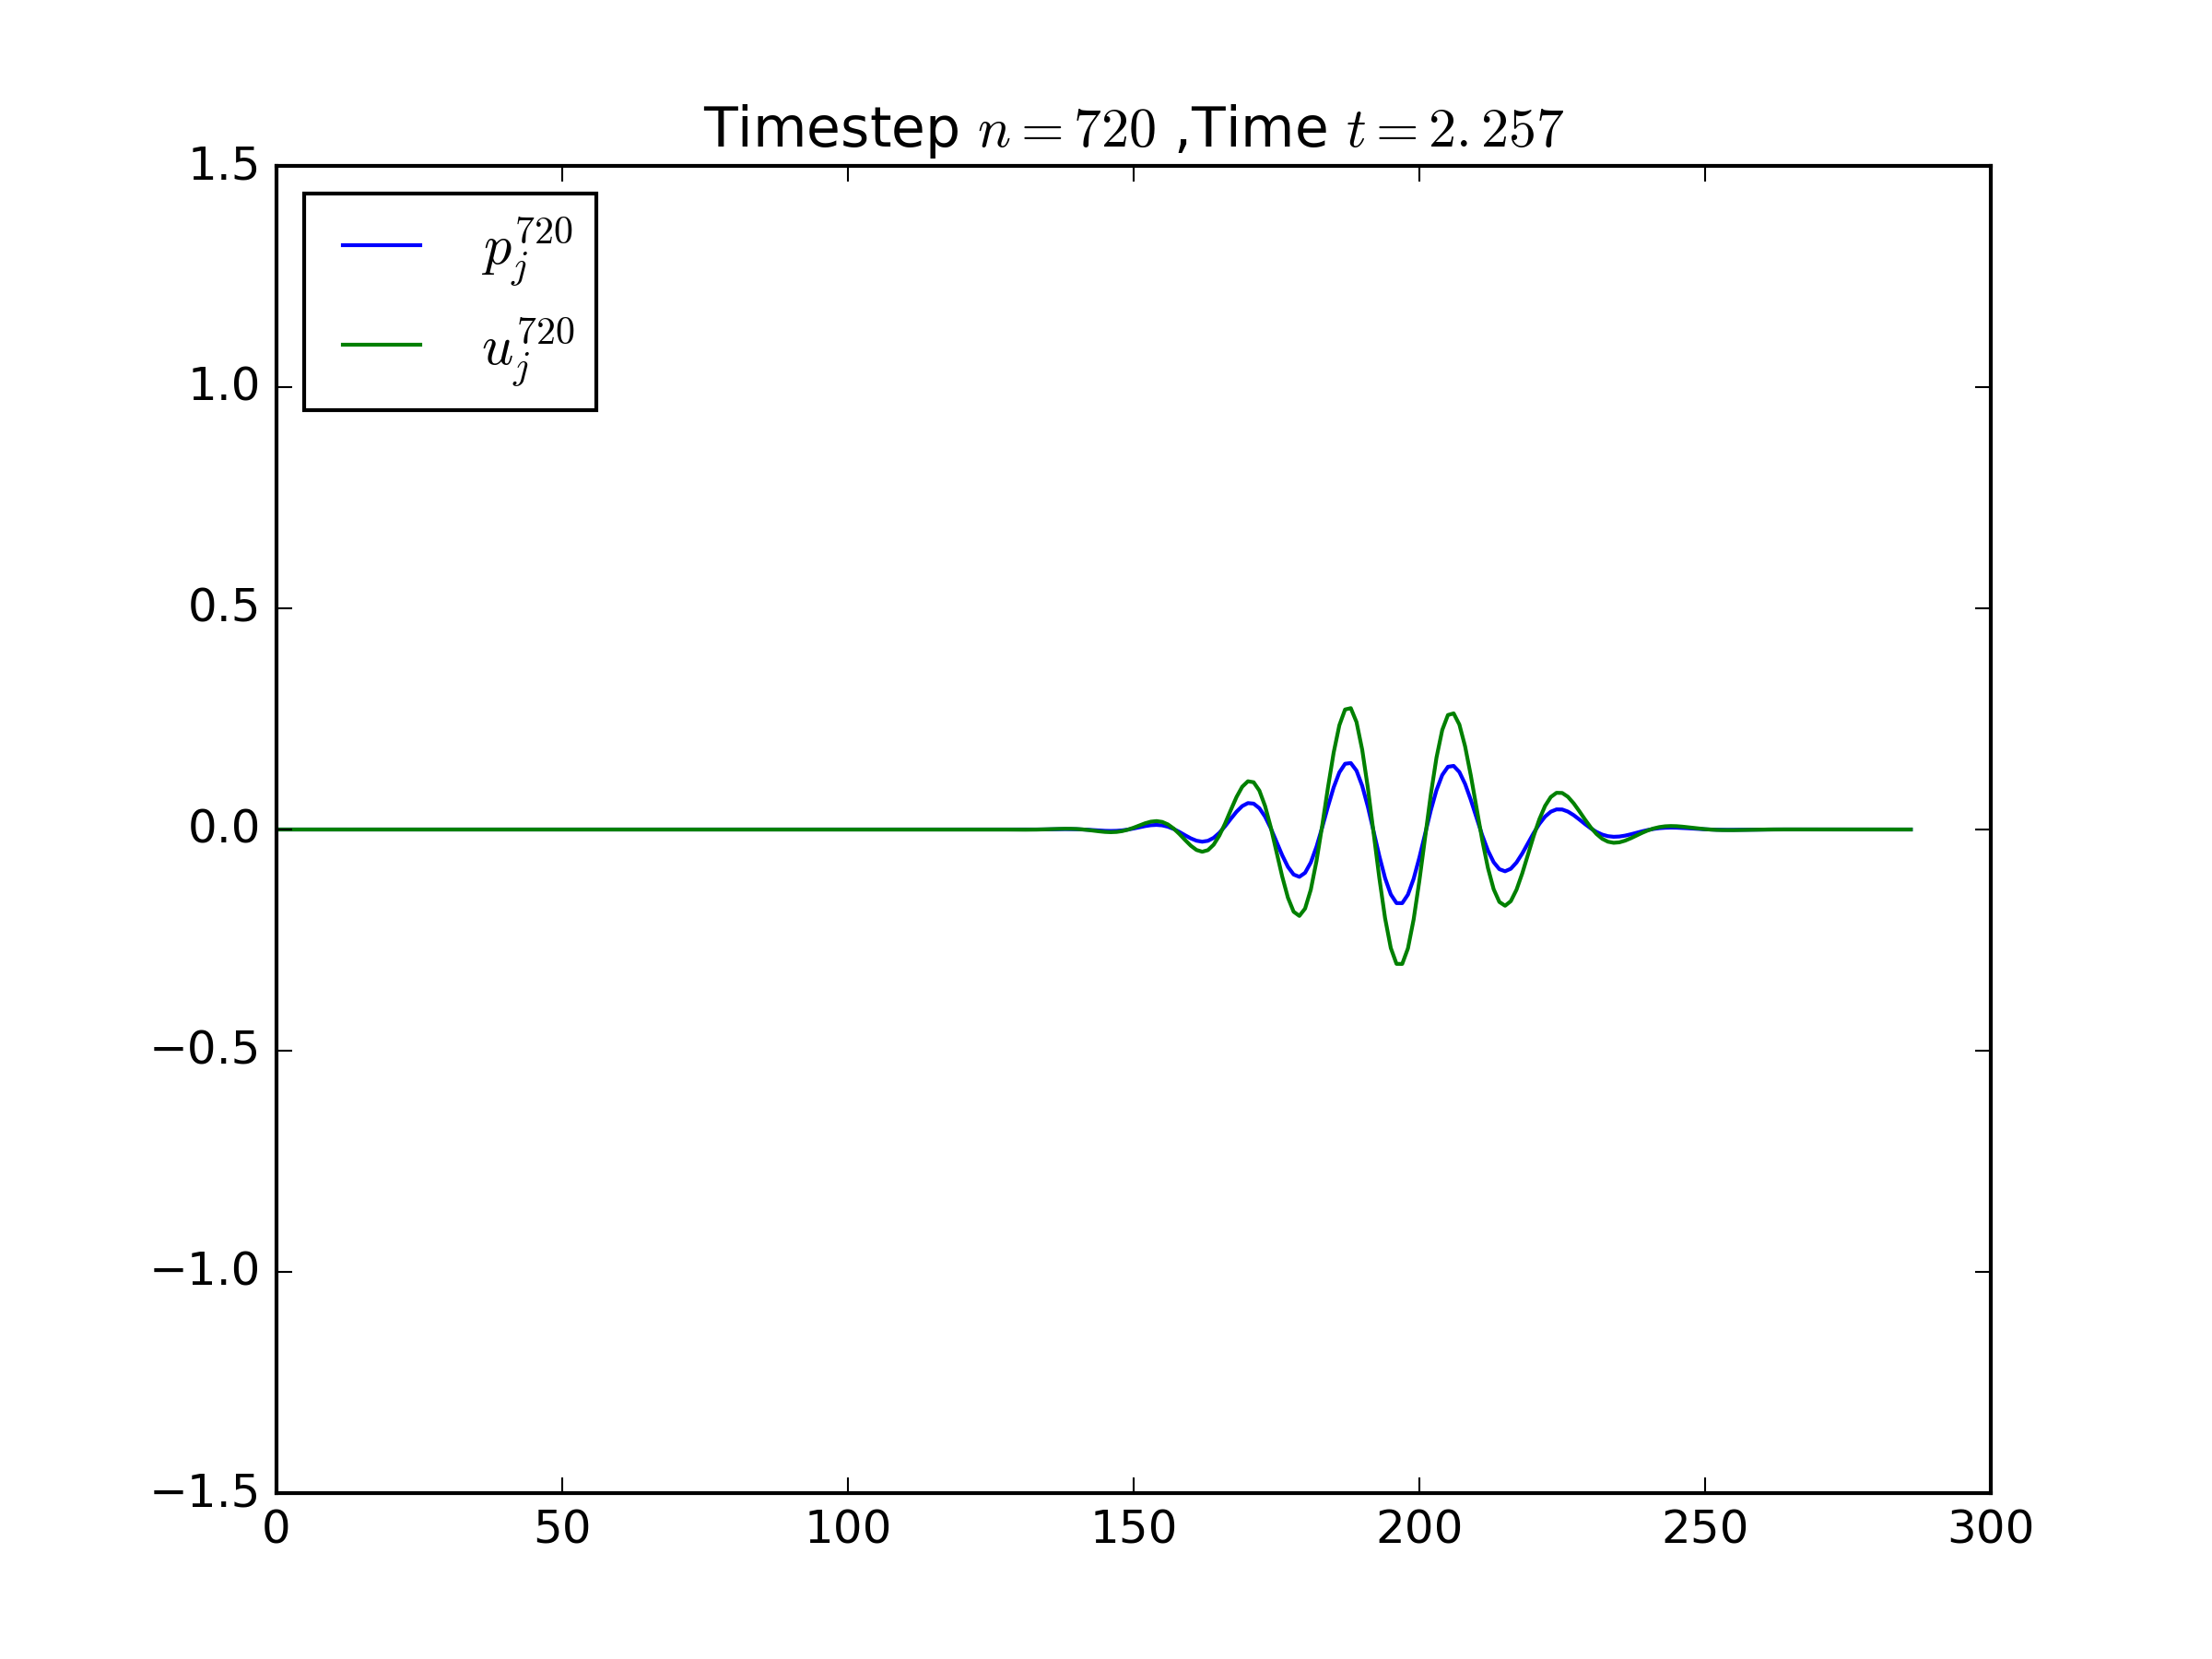
\includegraphics[width=0.31\textwidth]{figures/problem_1_a_072.png}
            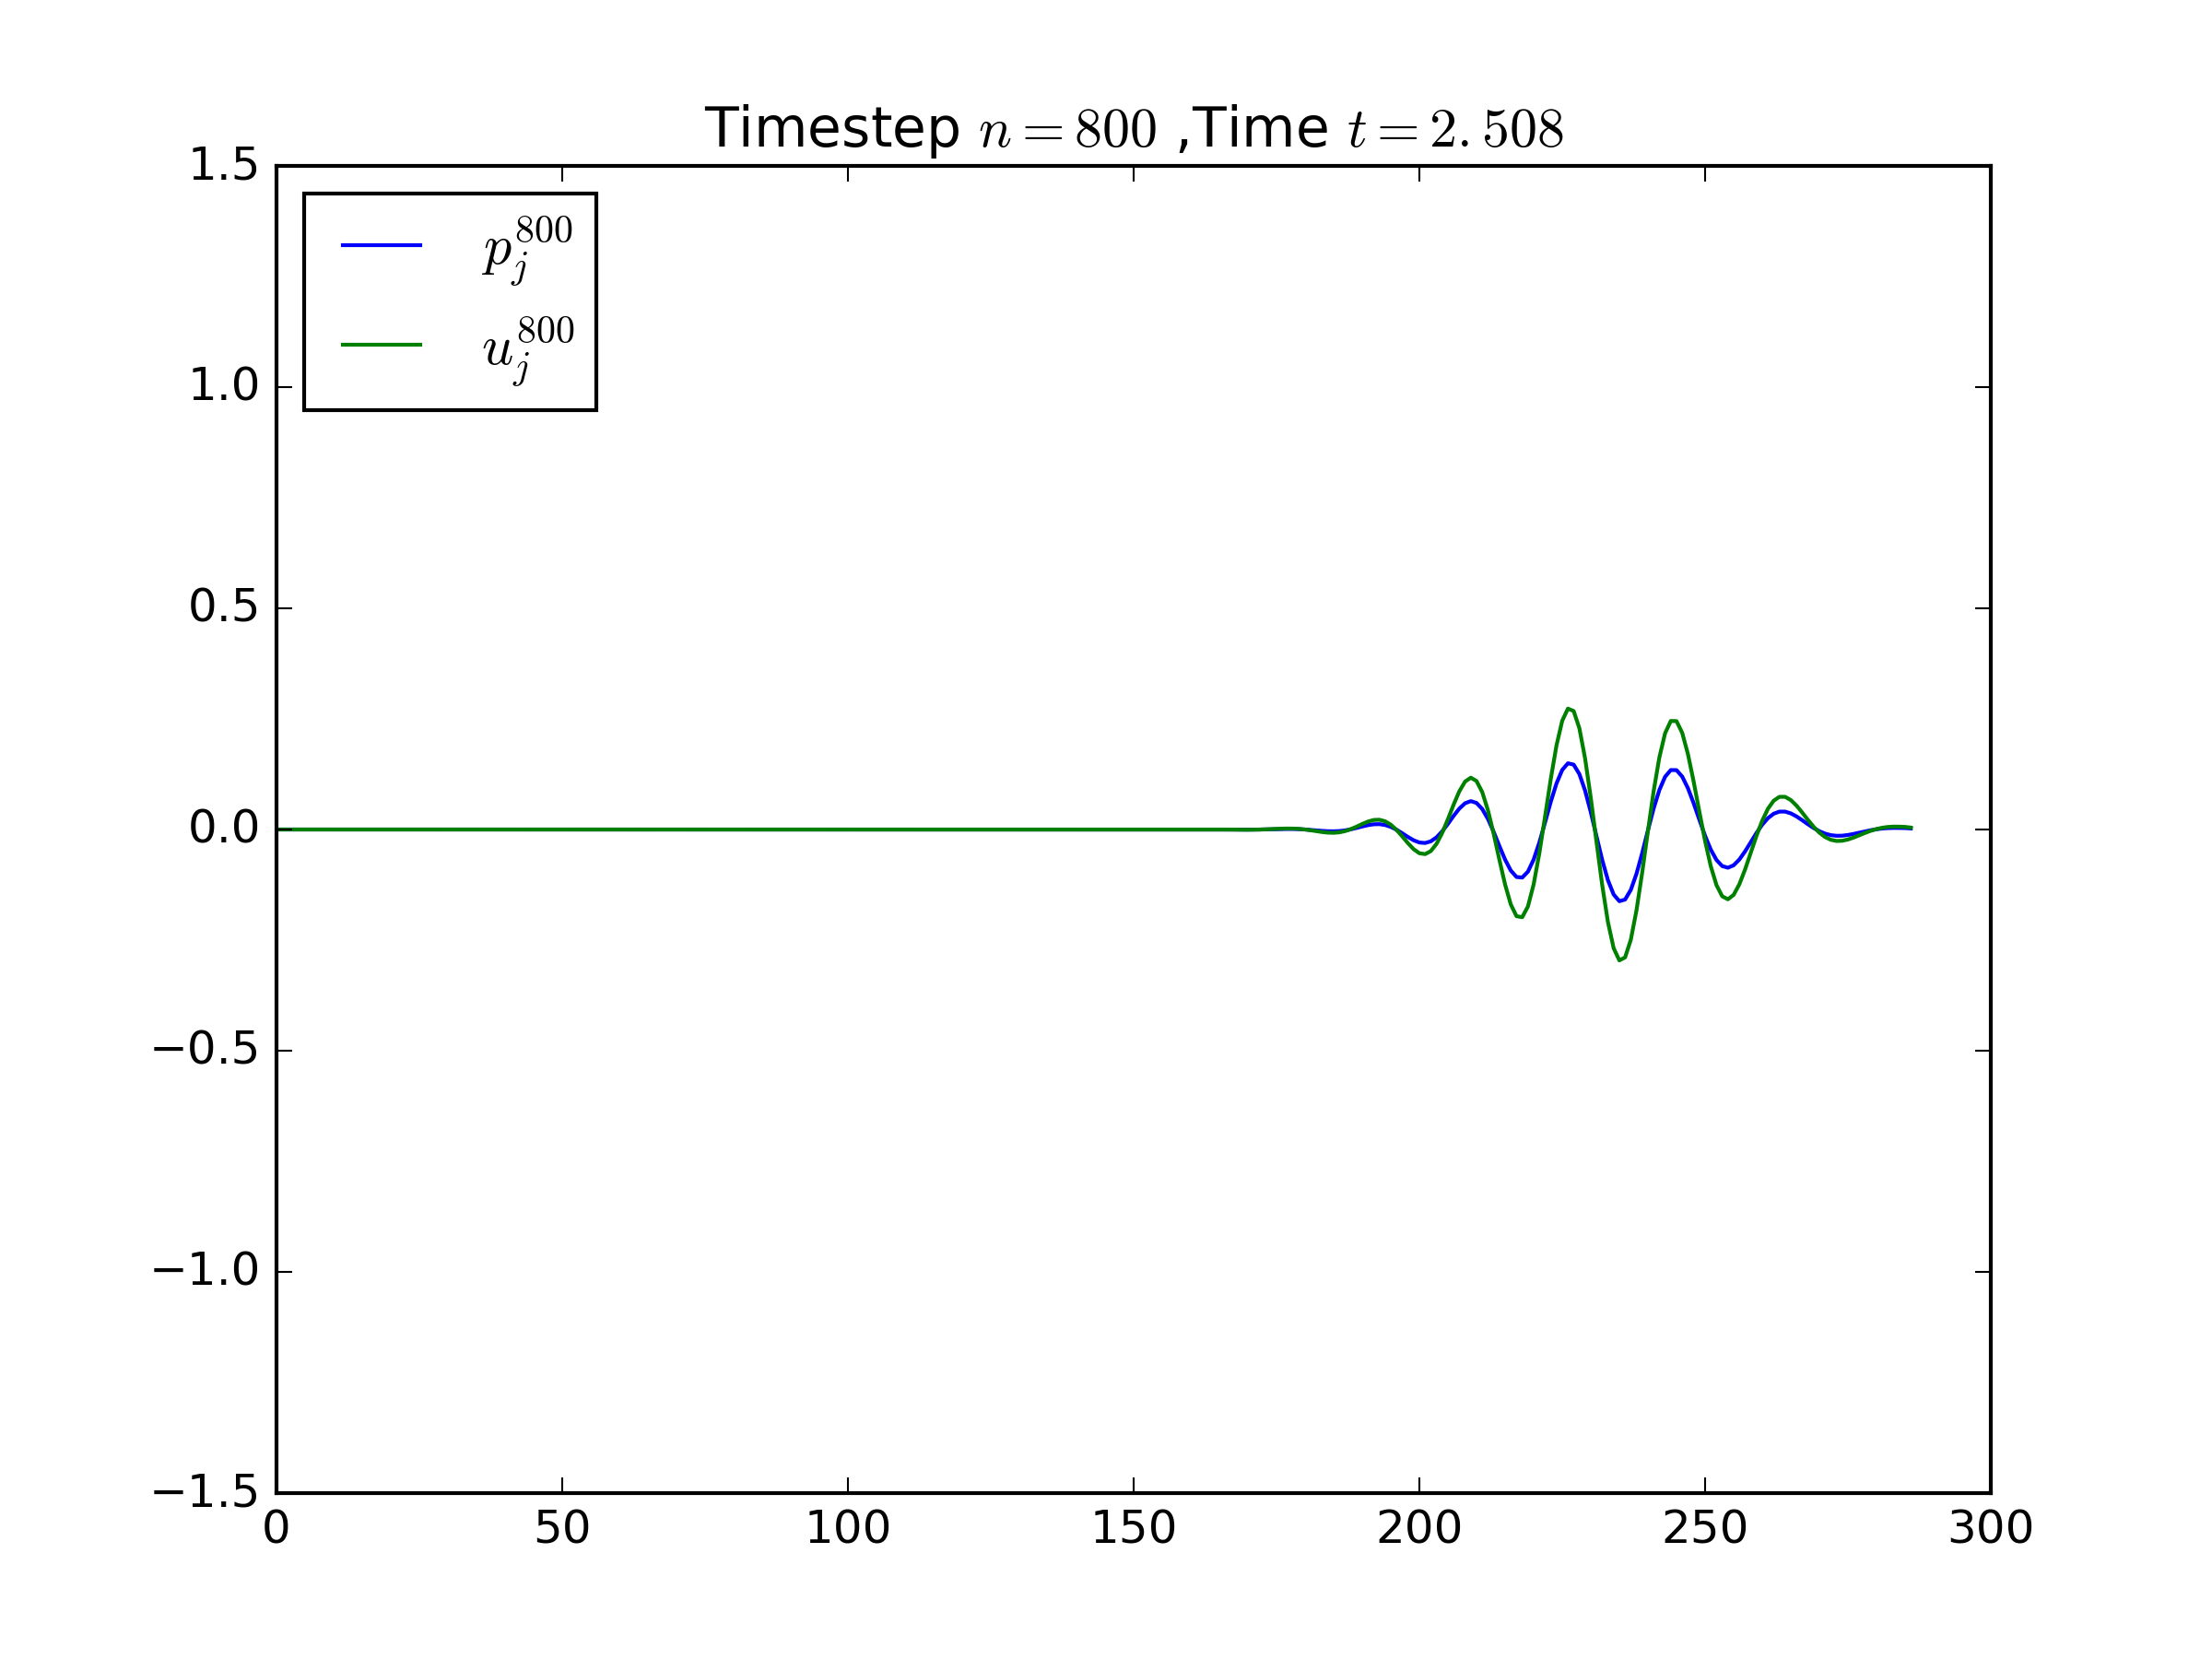
\includegraphics[width=0.31\textwidth]{figures/problem_1_a_080.png}
            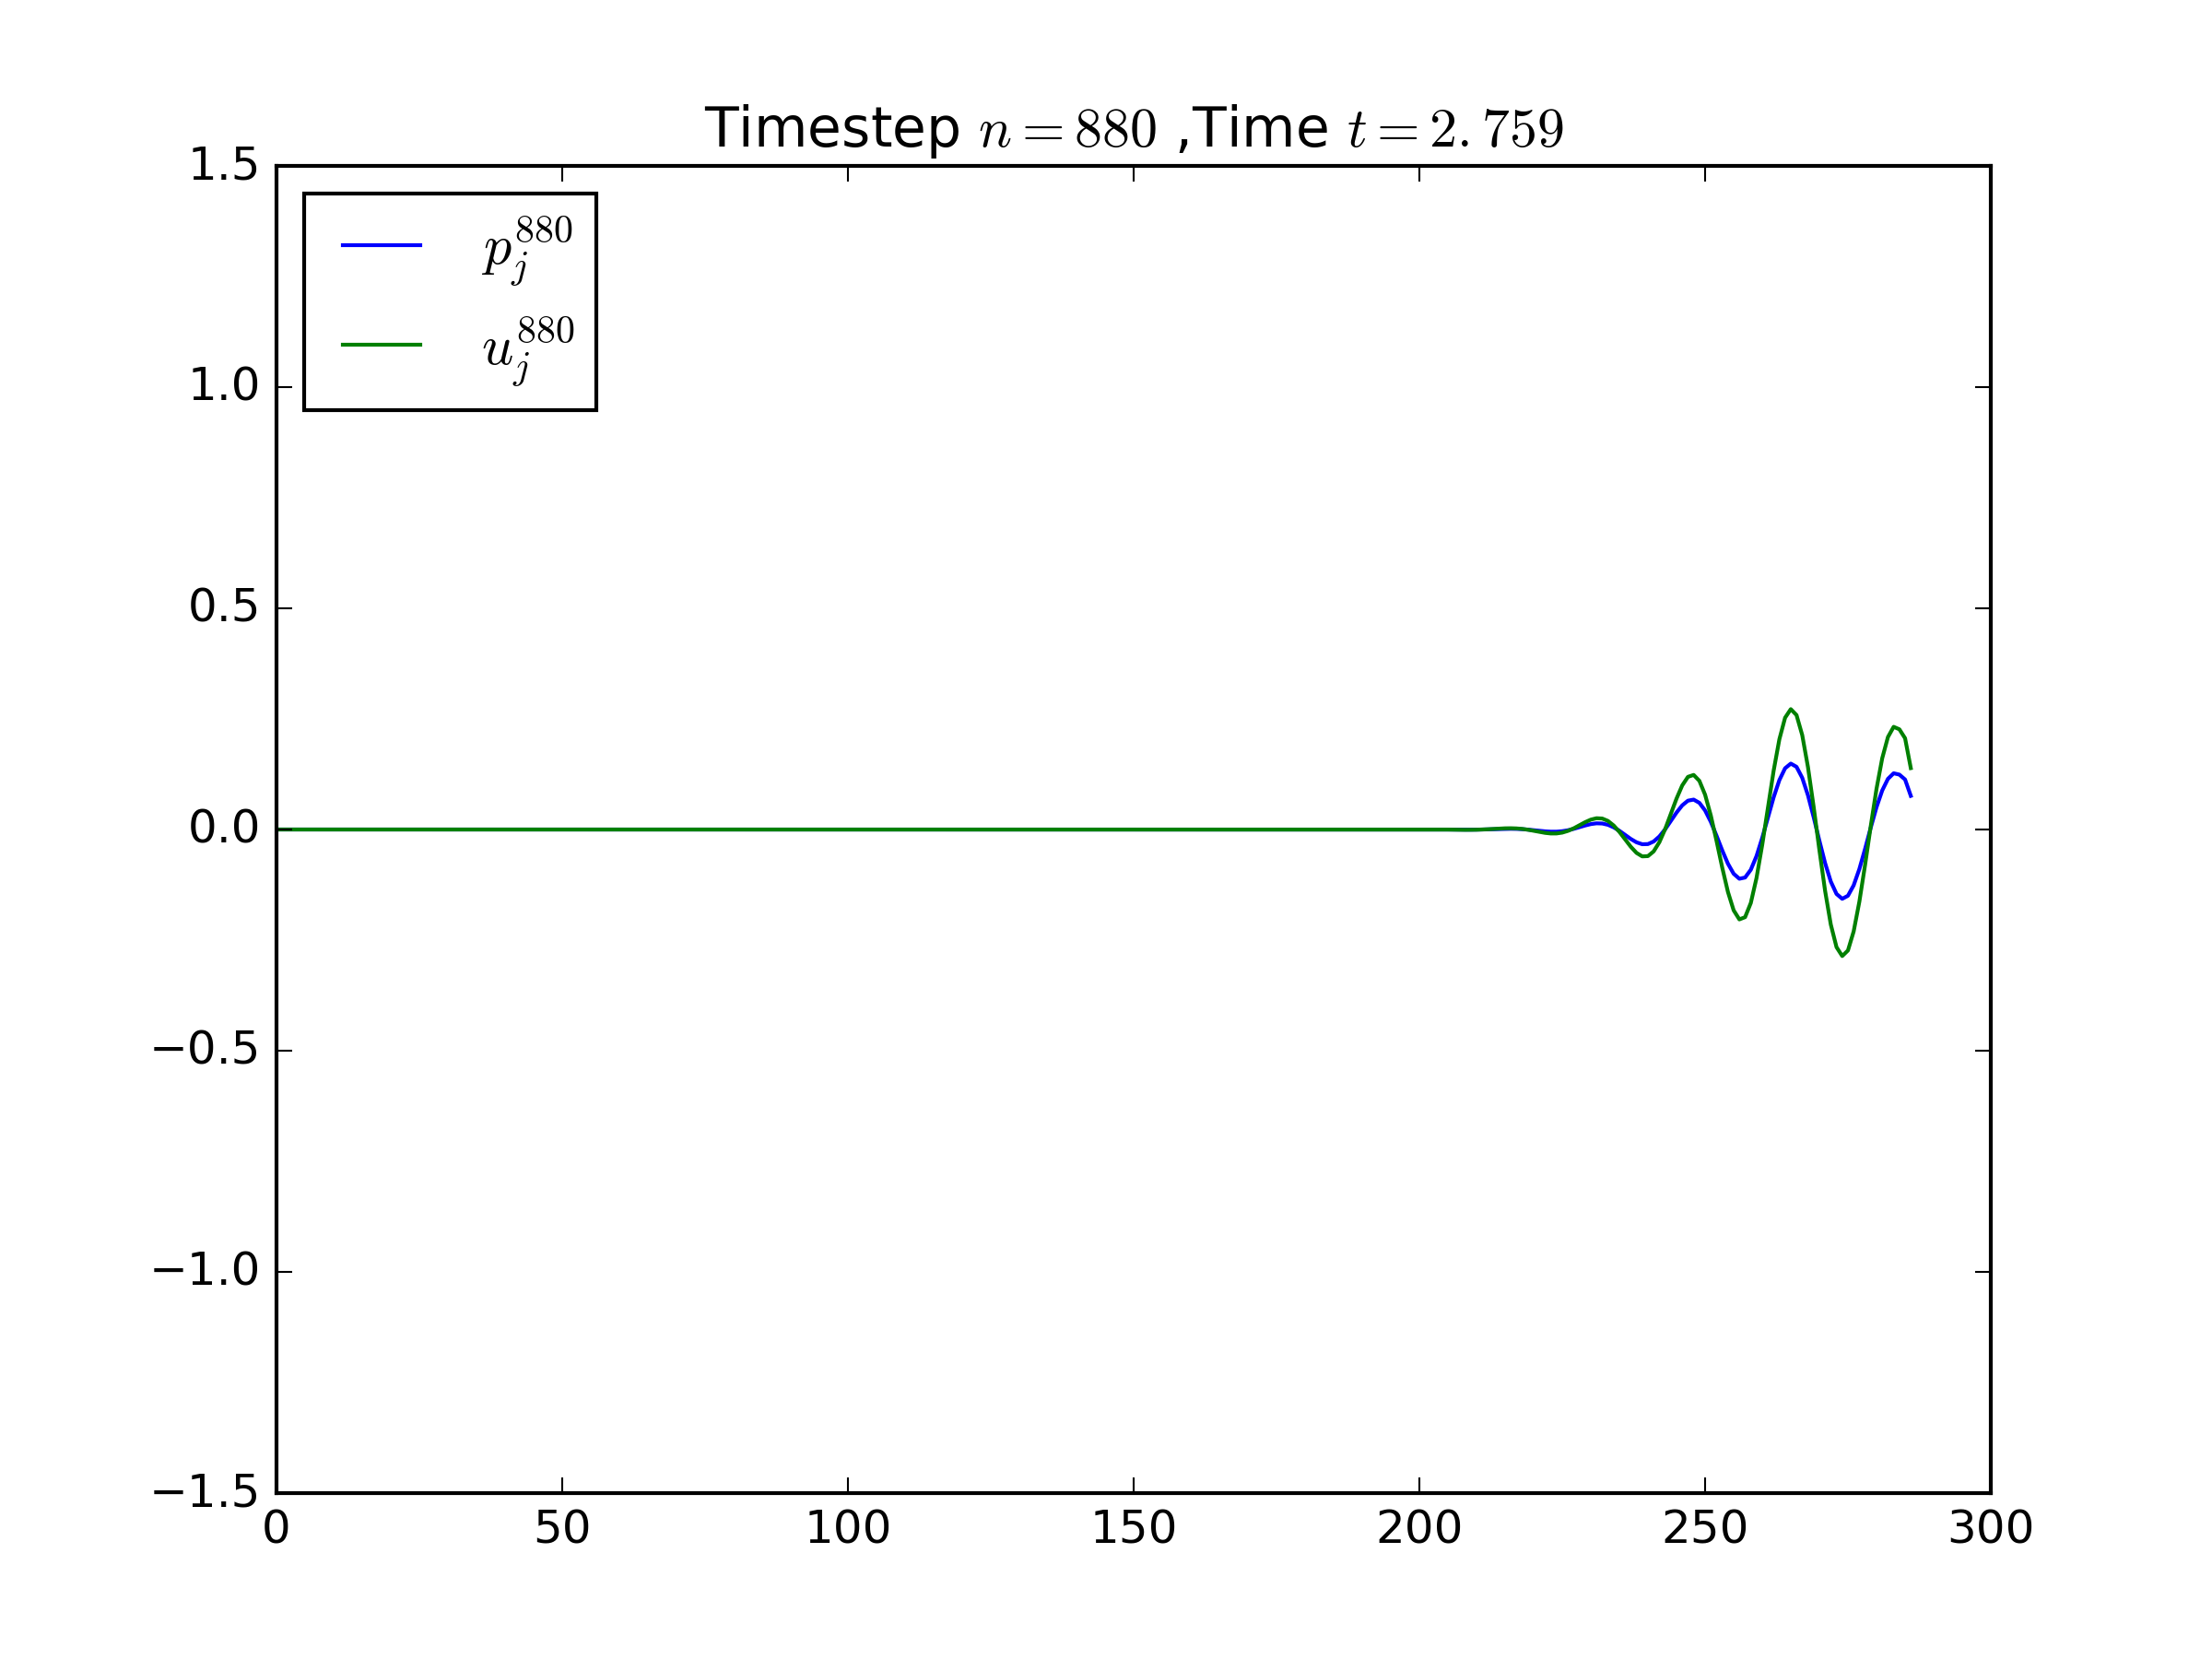
\includegraphics[width=0.31\textwidth]{figures/problem_1_a_088.png}
            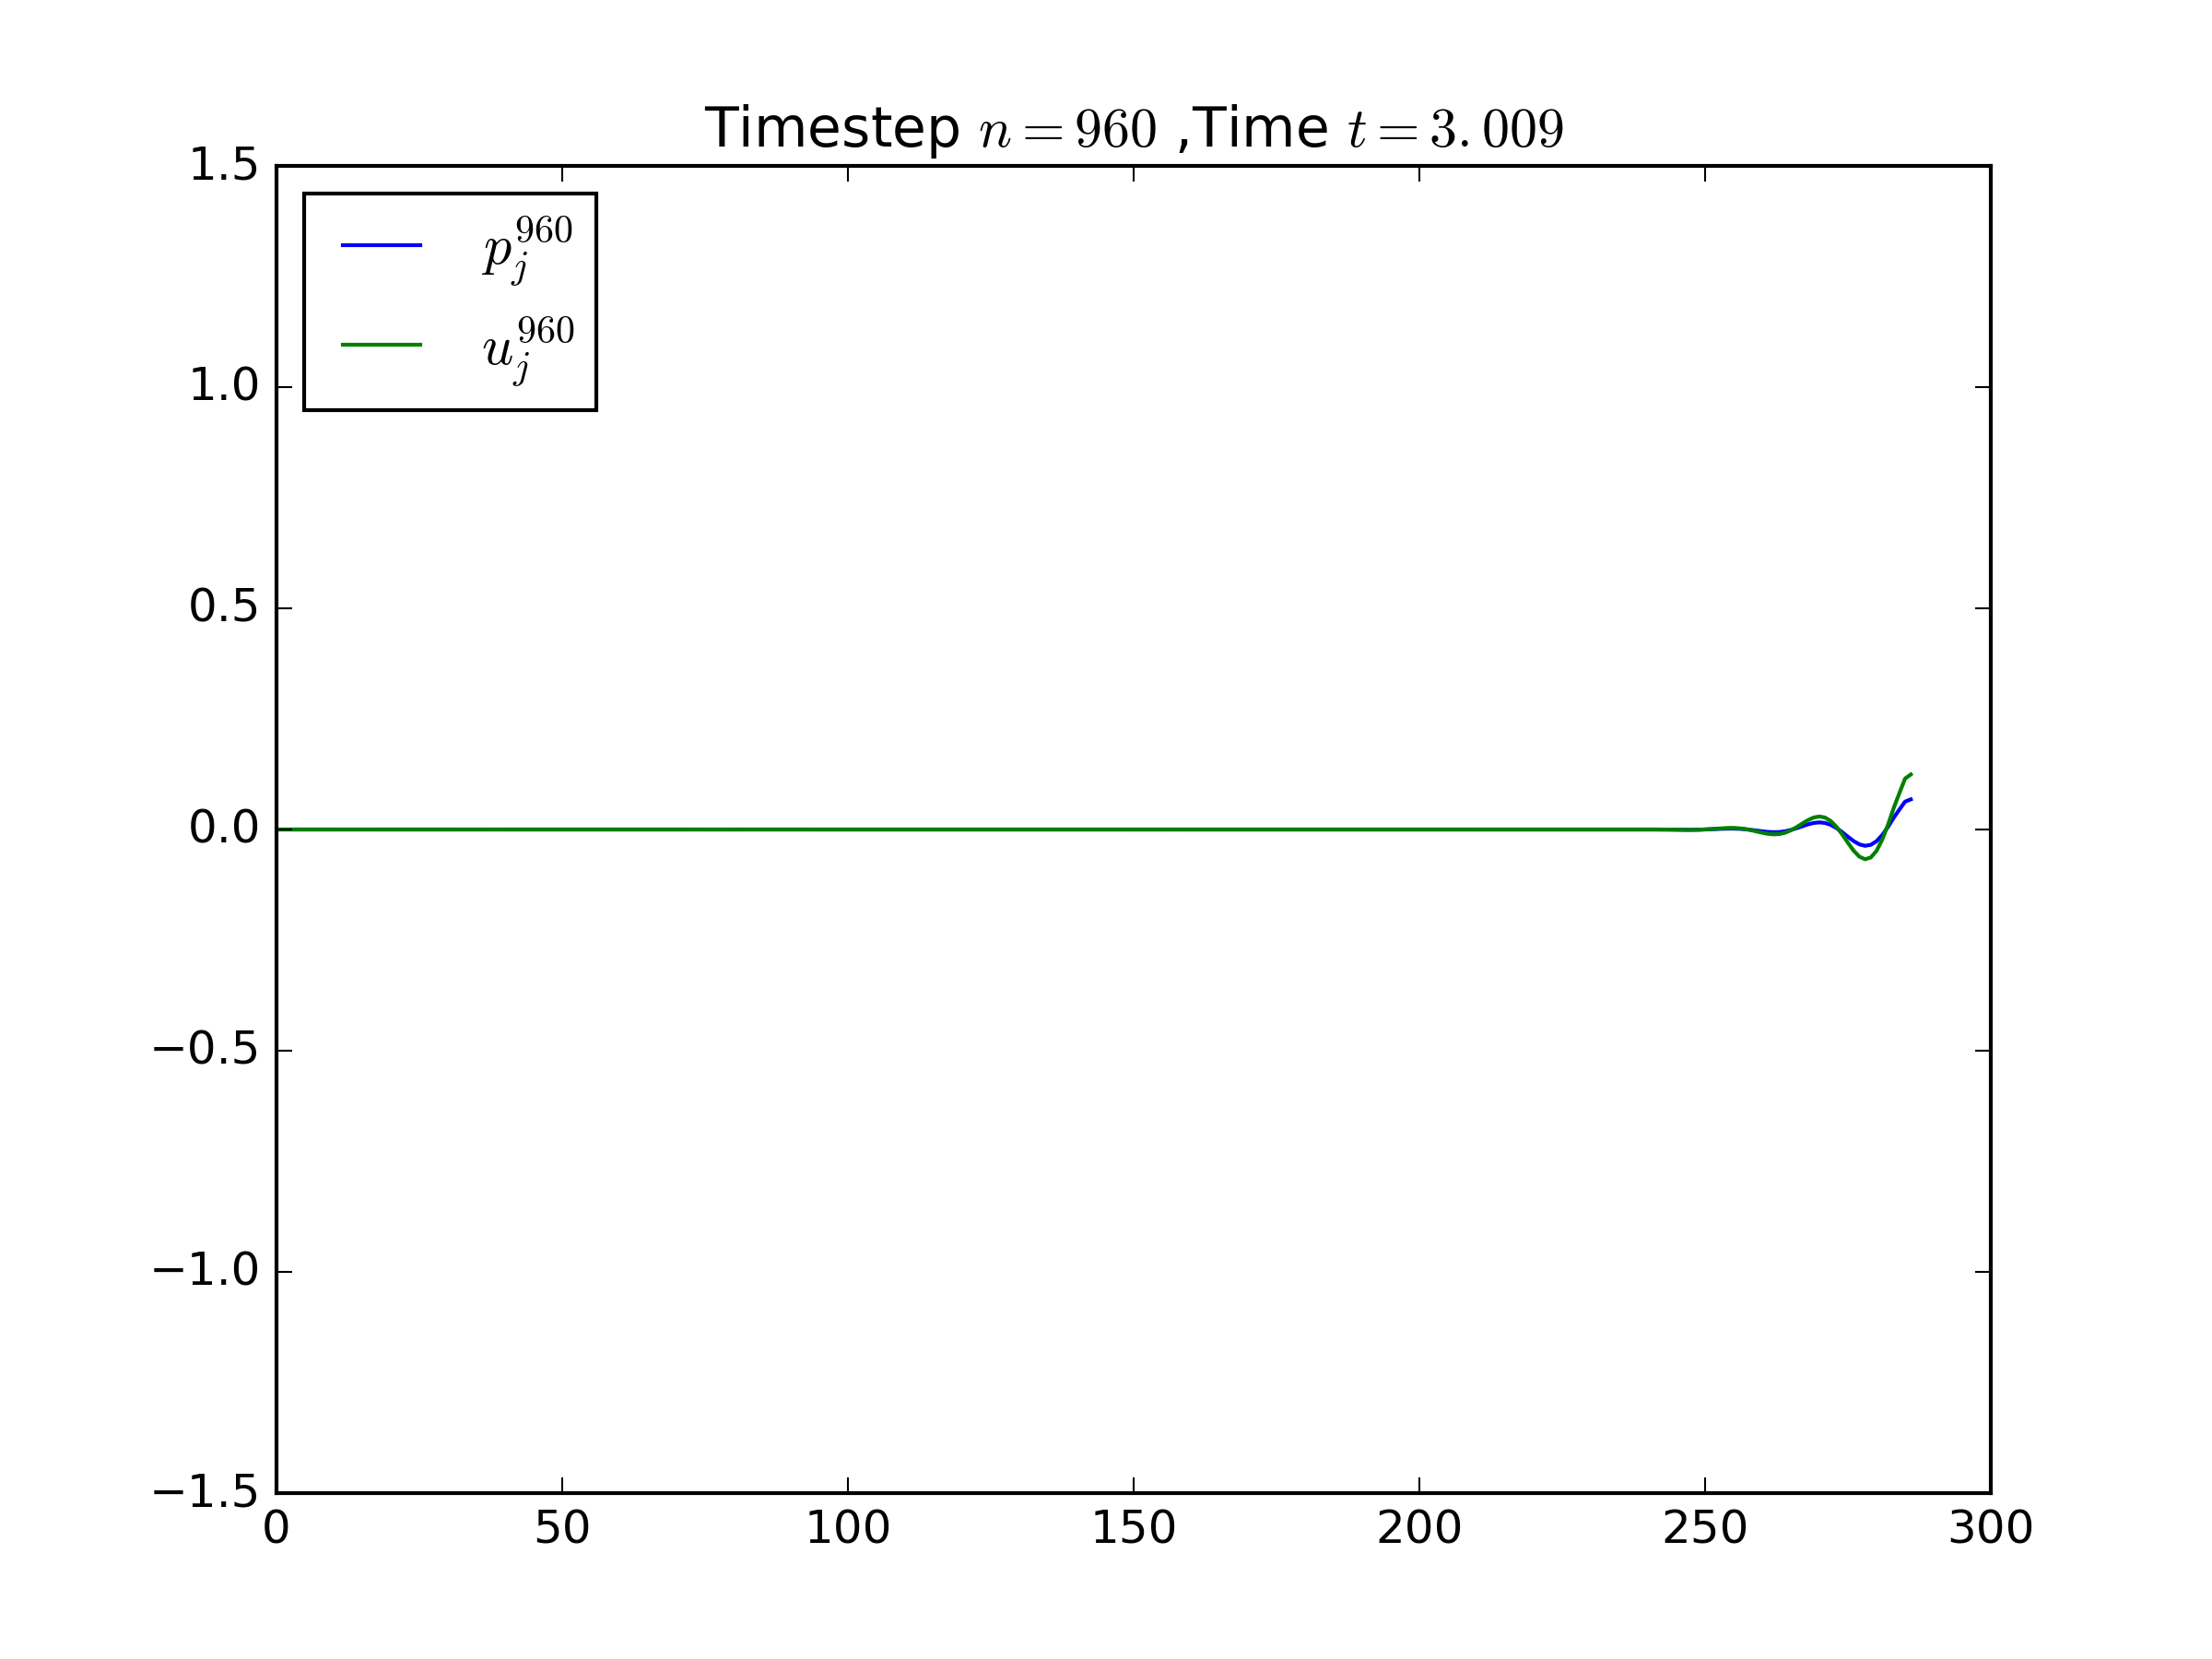
\includegraphics[width=0.31\textwidth]{figures/problem_1_a_096.png}
            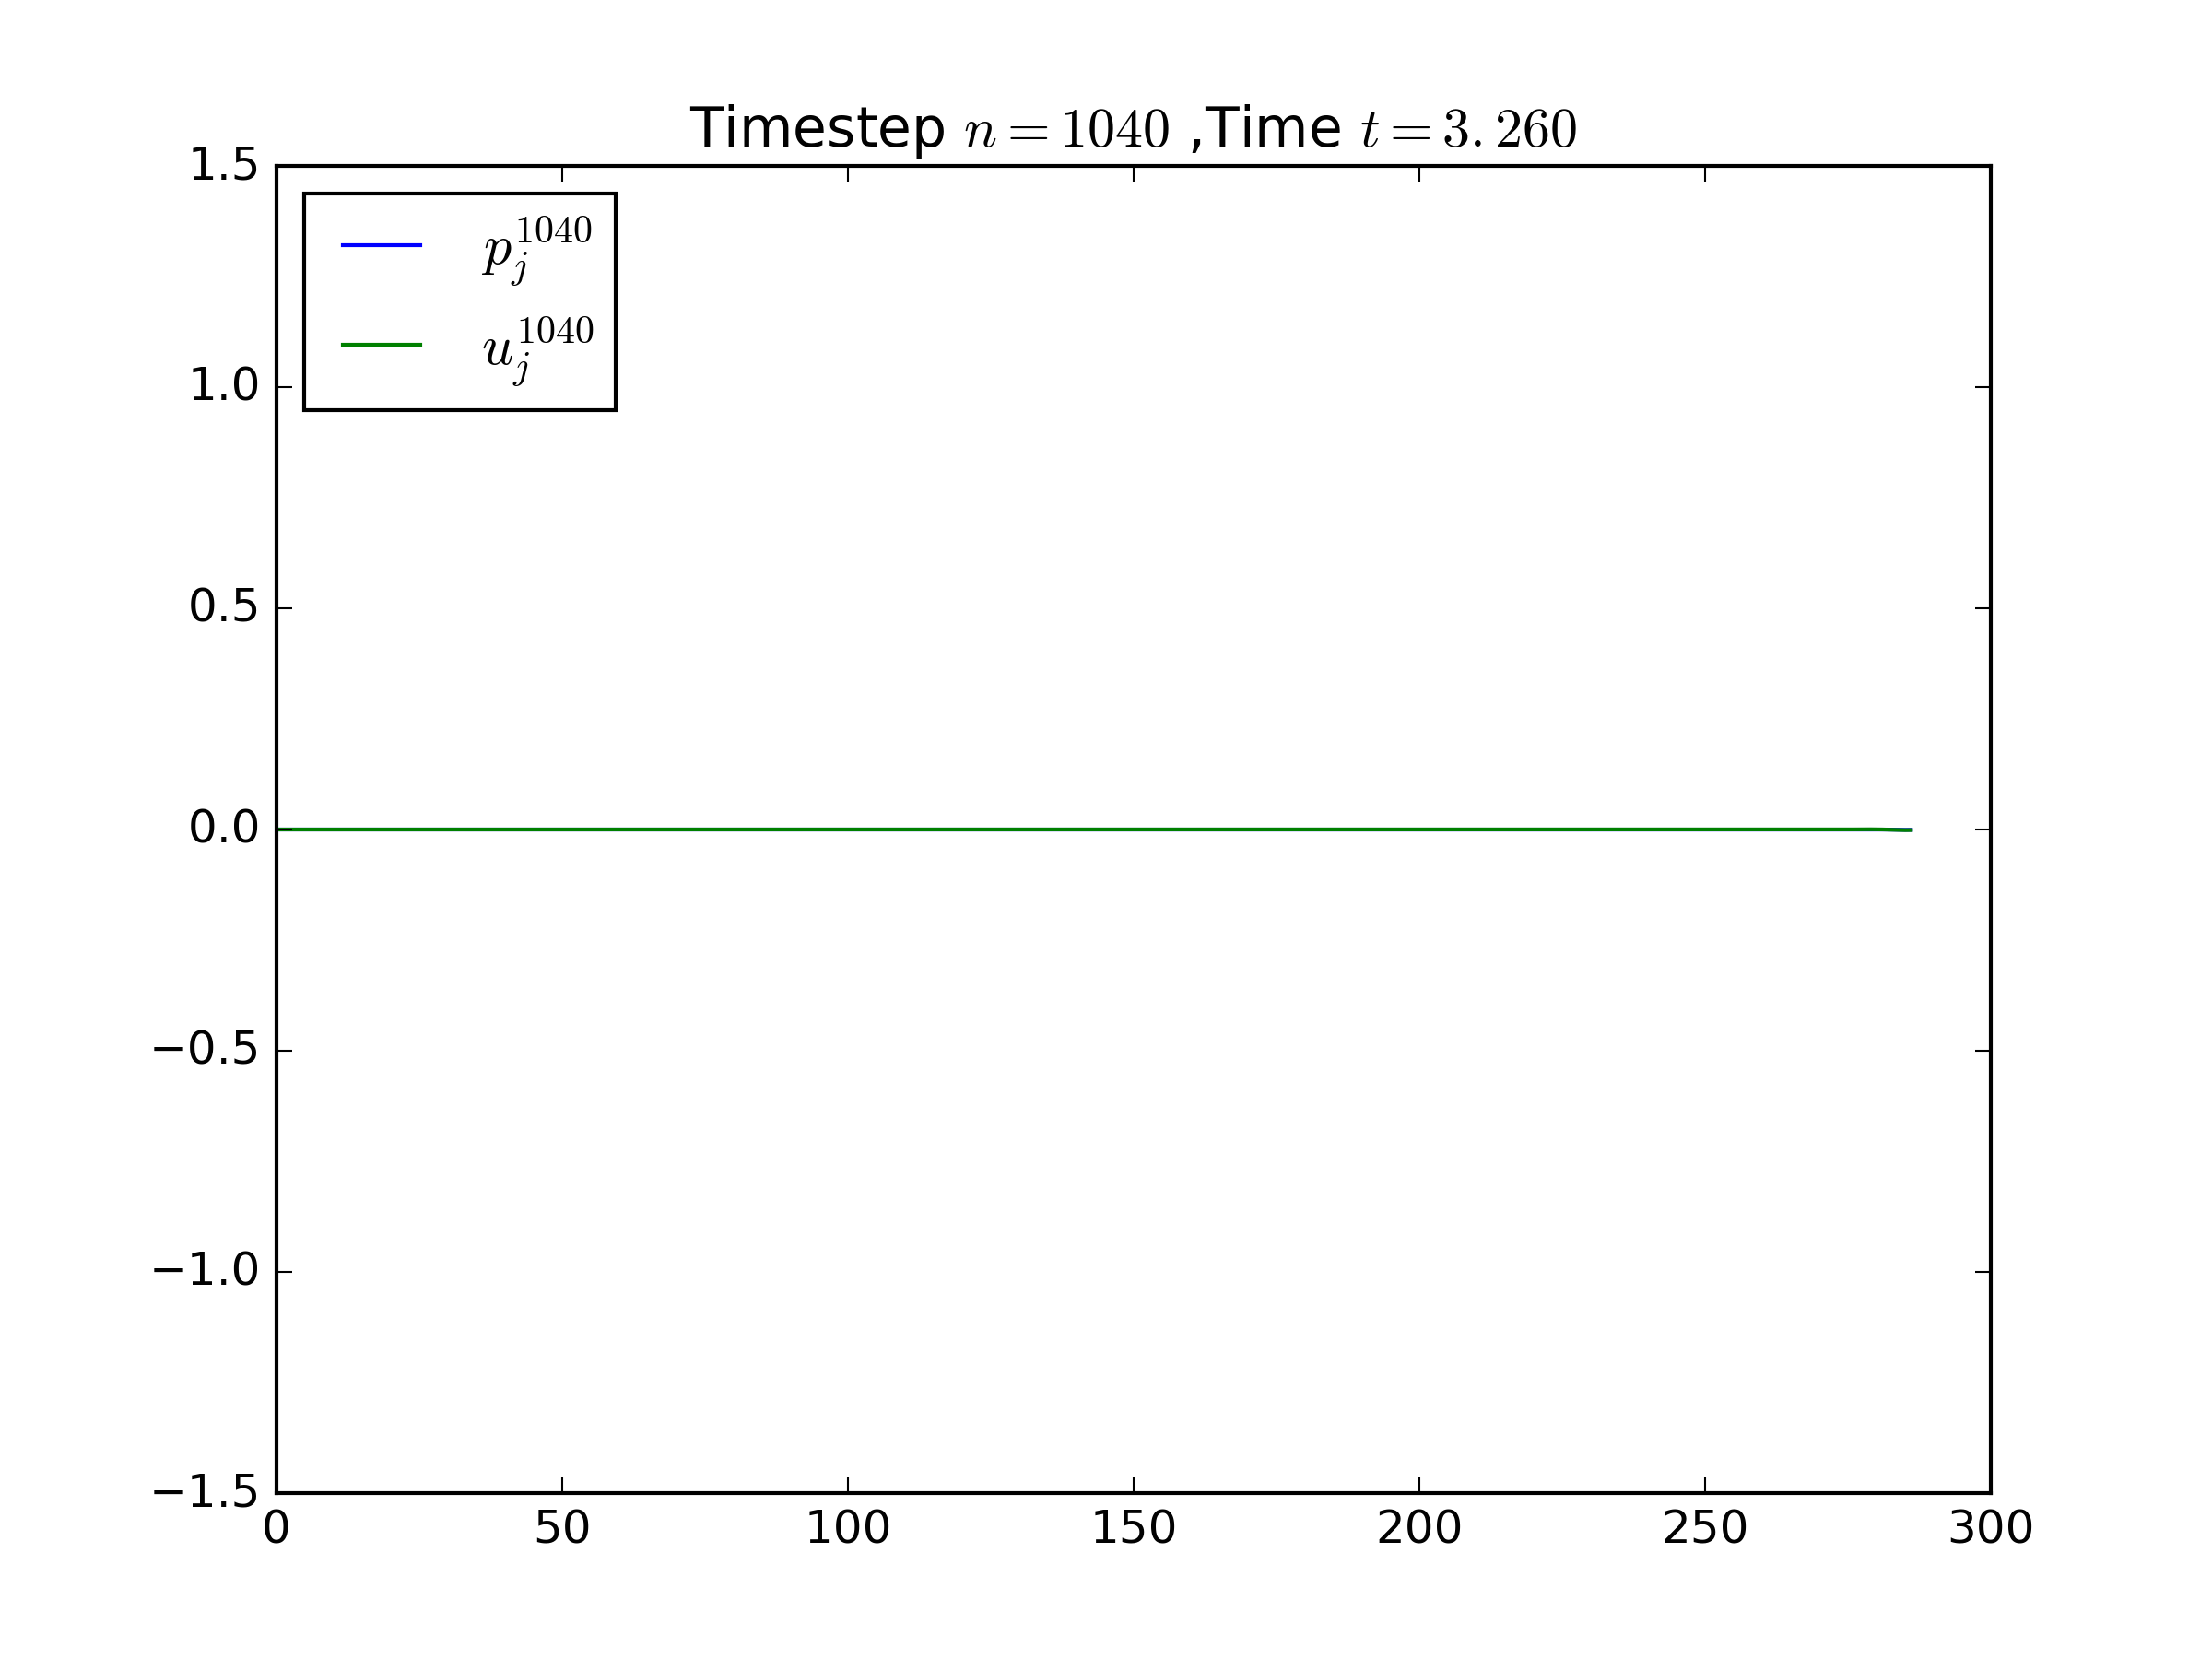
\includegraphics[width=0.31\textwidth]{figures/problem_1_a_104.png}
            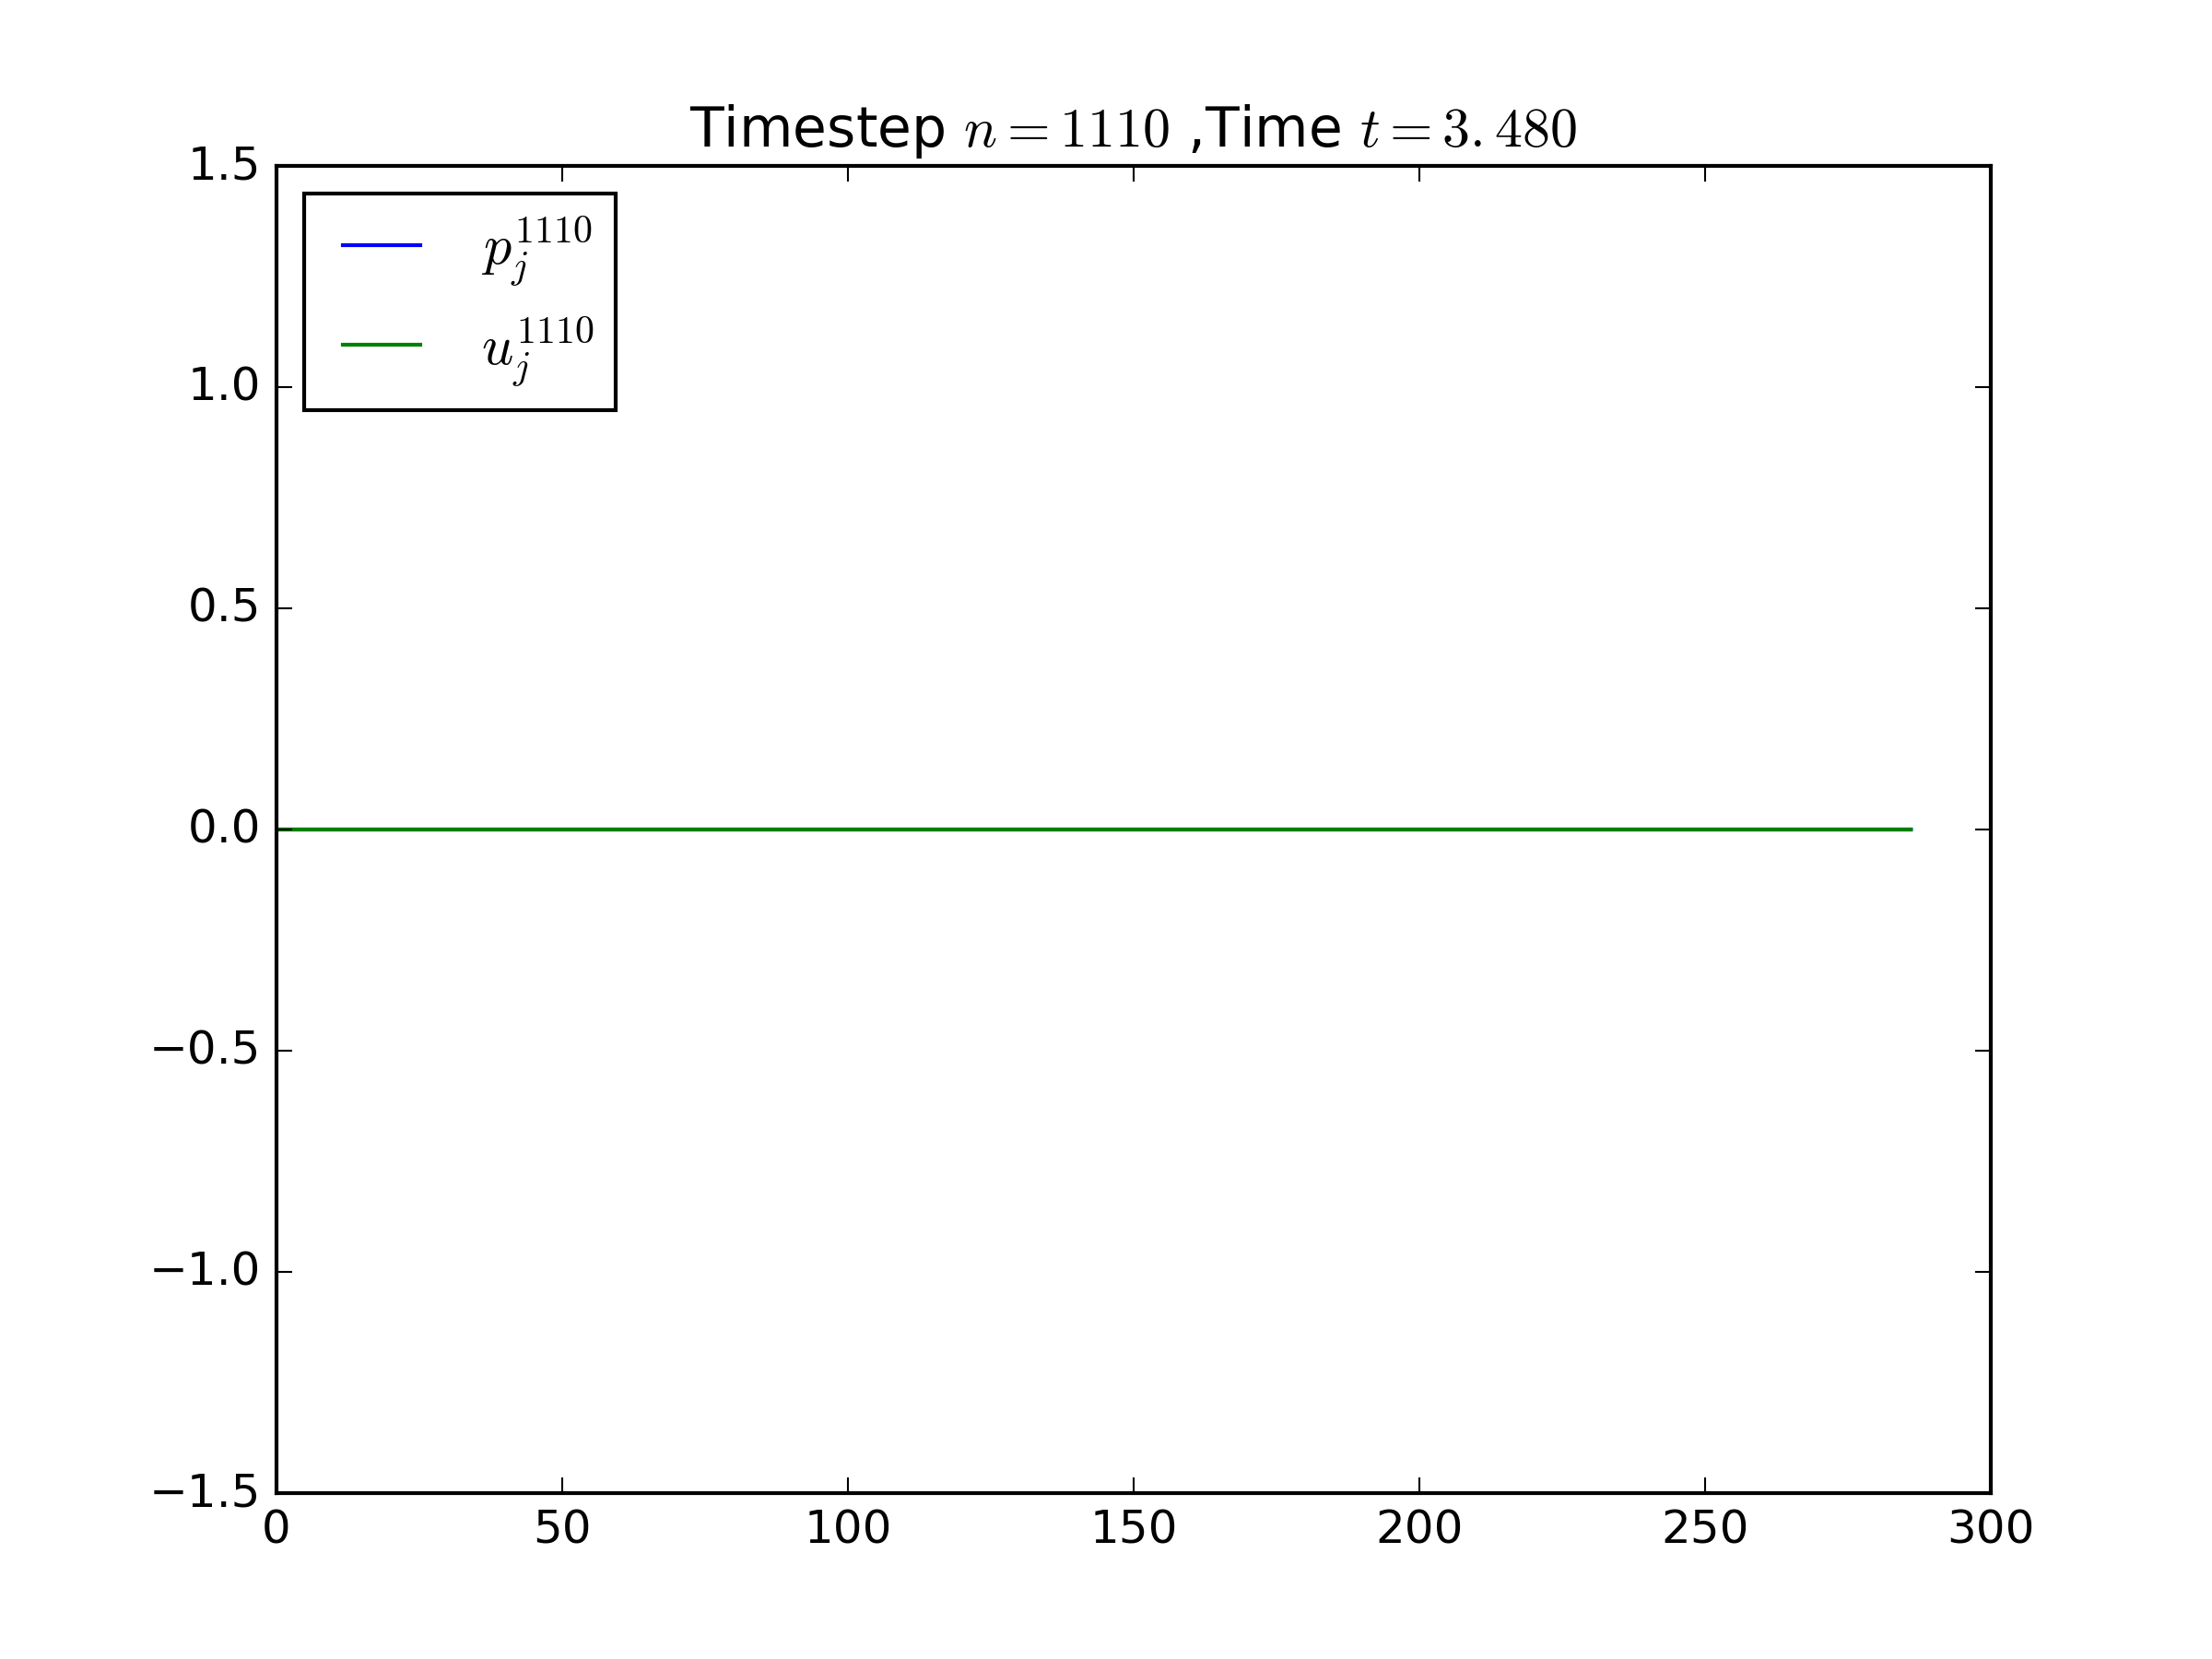
\includegraphics[width=0.31\textwidth]{figures/problem_1_a_111.png}
        \end{figure}
        \FloatBarrier
        Clearly we see the waves move to both the left and right, but the wave to the left is significantly smaller.  When the large wave hits the right border, it is dissipated in to a very small wave moving left, but most of the ``stuff'' leaves the system.  When the smaller wave hits the left border, it bounces back and moves right.  Notice the $u$ wave is flipped when it hits the left side since we are assuming the boundary condition $u_0^n = -u_1^n$.  Finally, the small wave endures the same fate as the initial larger wave: it leaves the system through the left border. \\

        The following figures show the movement of a step function.  The same general behavior is seen in this simulation.  Note that the step function shape is not well-preserved because Lax-Wendroff is not a good method for discontinuous data (see Problem 2).
        \begin{figure}[ht!]
            \centering
            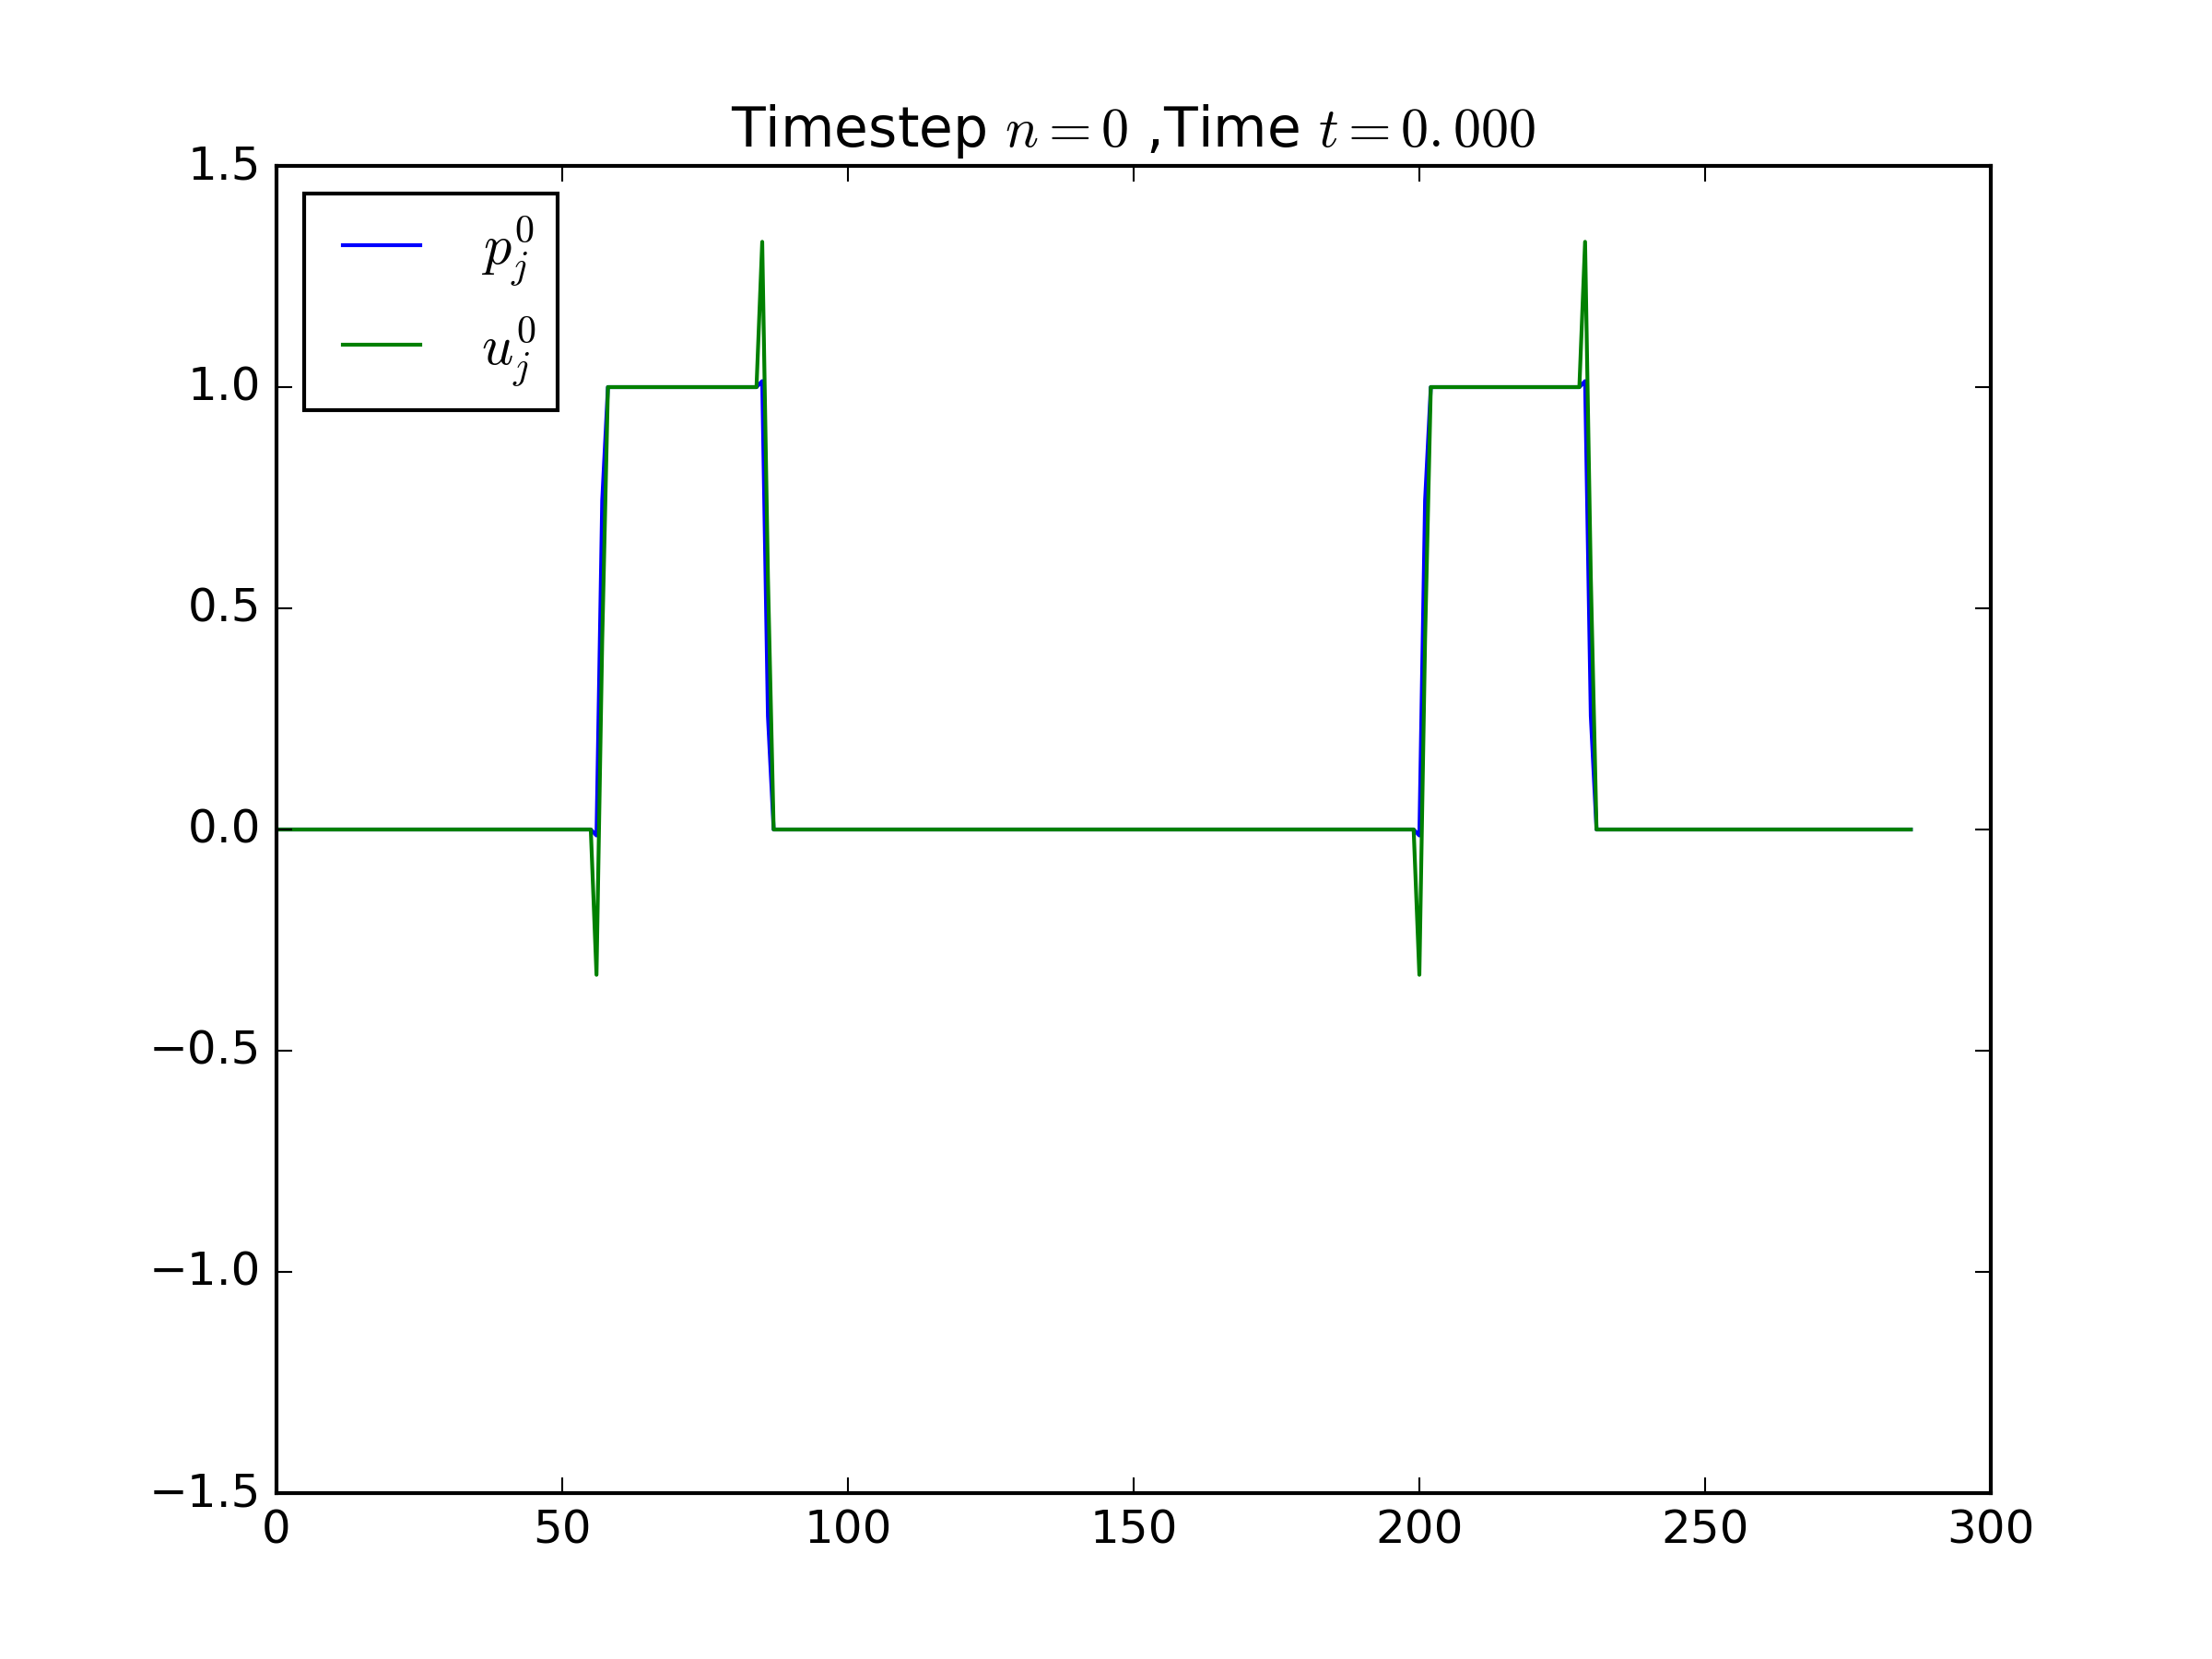
\includegraphics[width=0.31\textwidth]{figures/problem_1_b_000.png}
            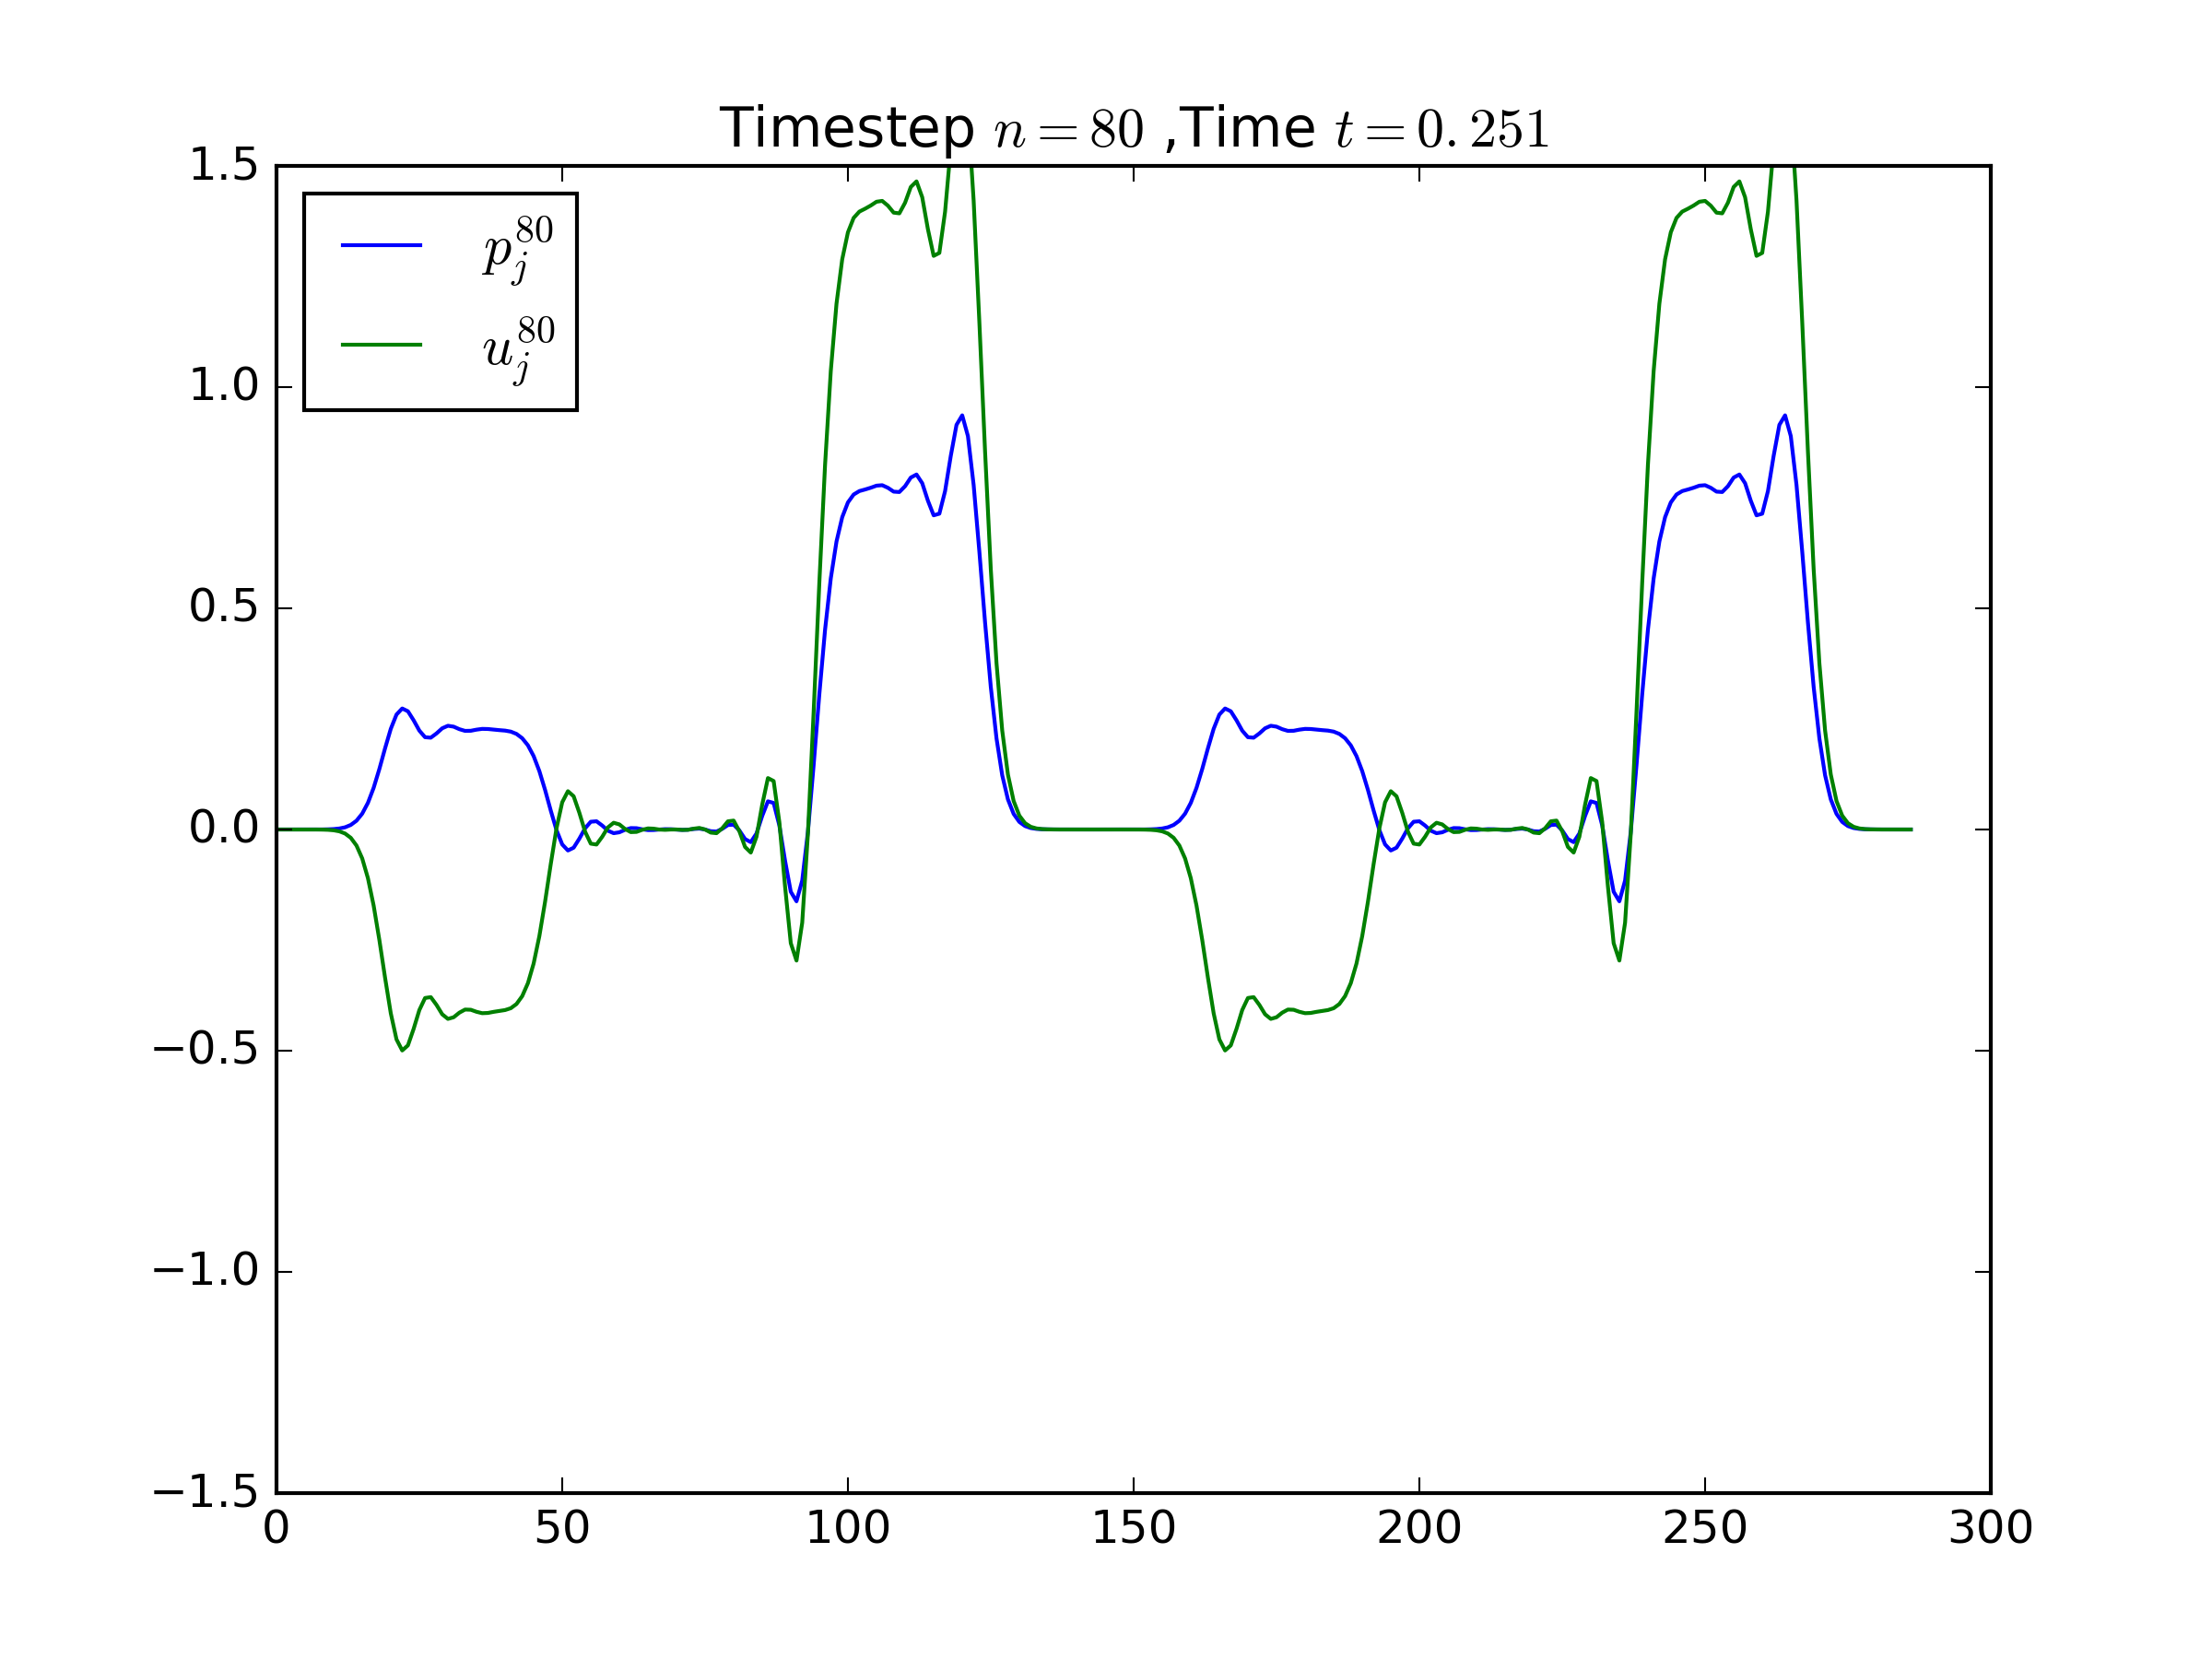
\includegraphics[width=0.31\textwidth]{figures/problem_1_b_008.png}
            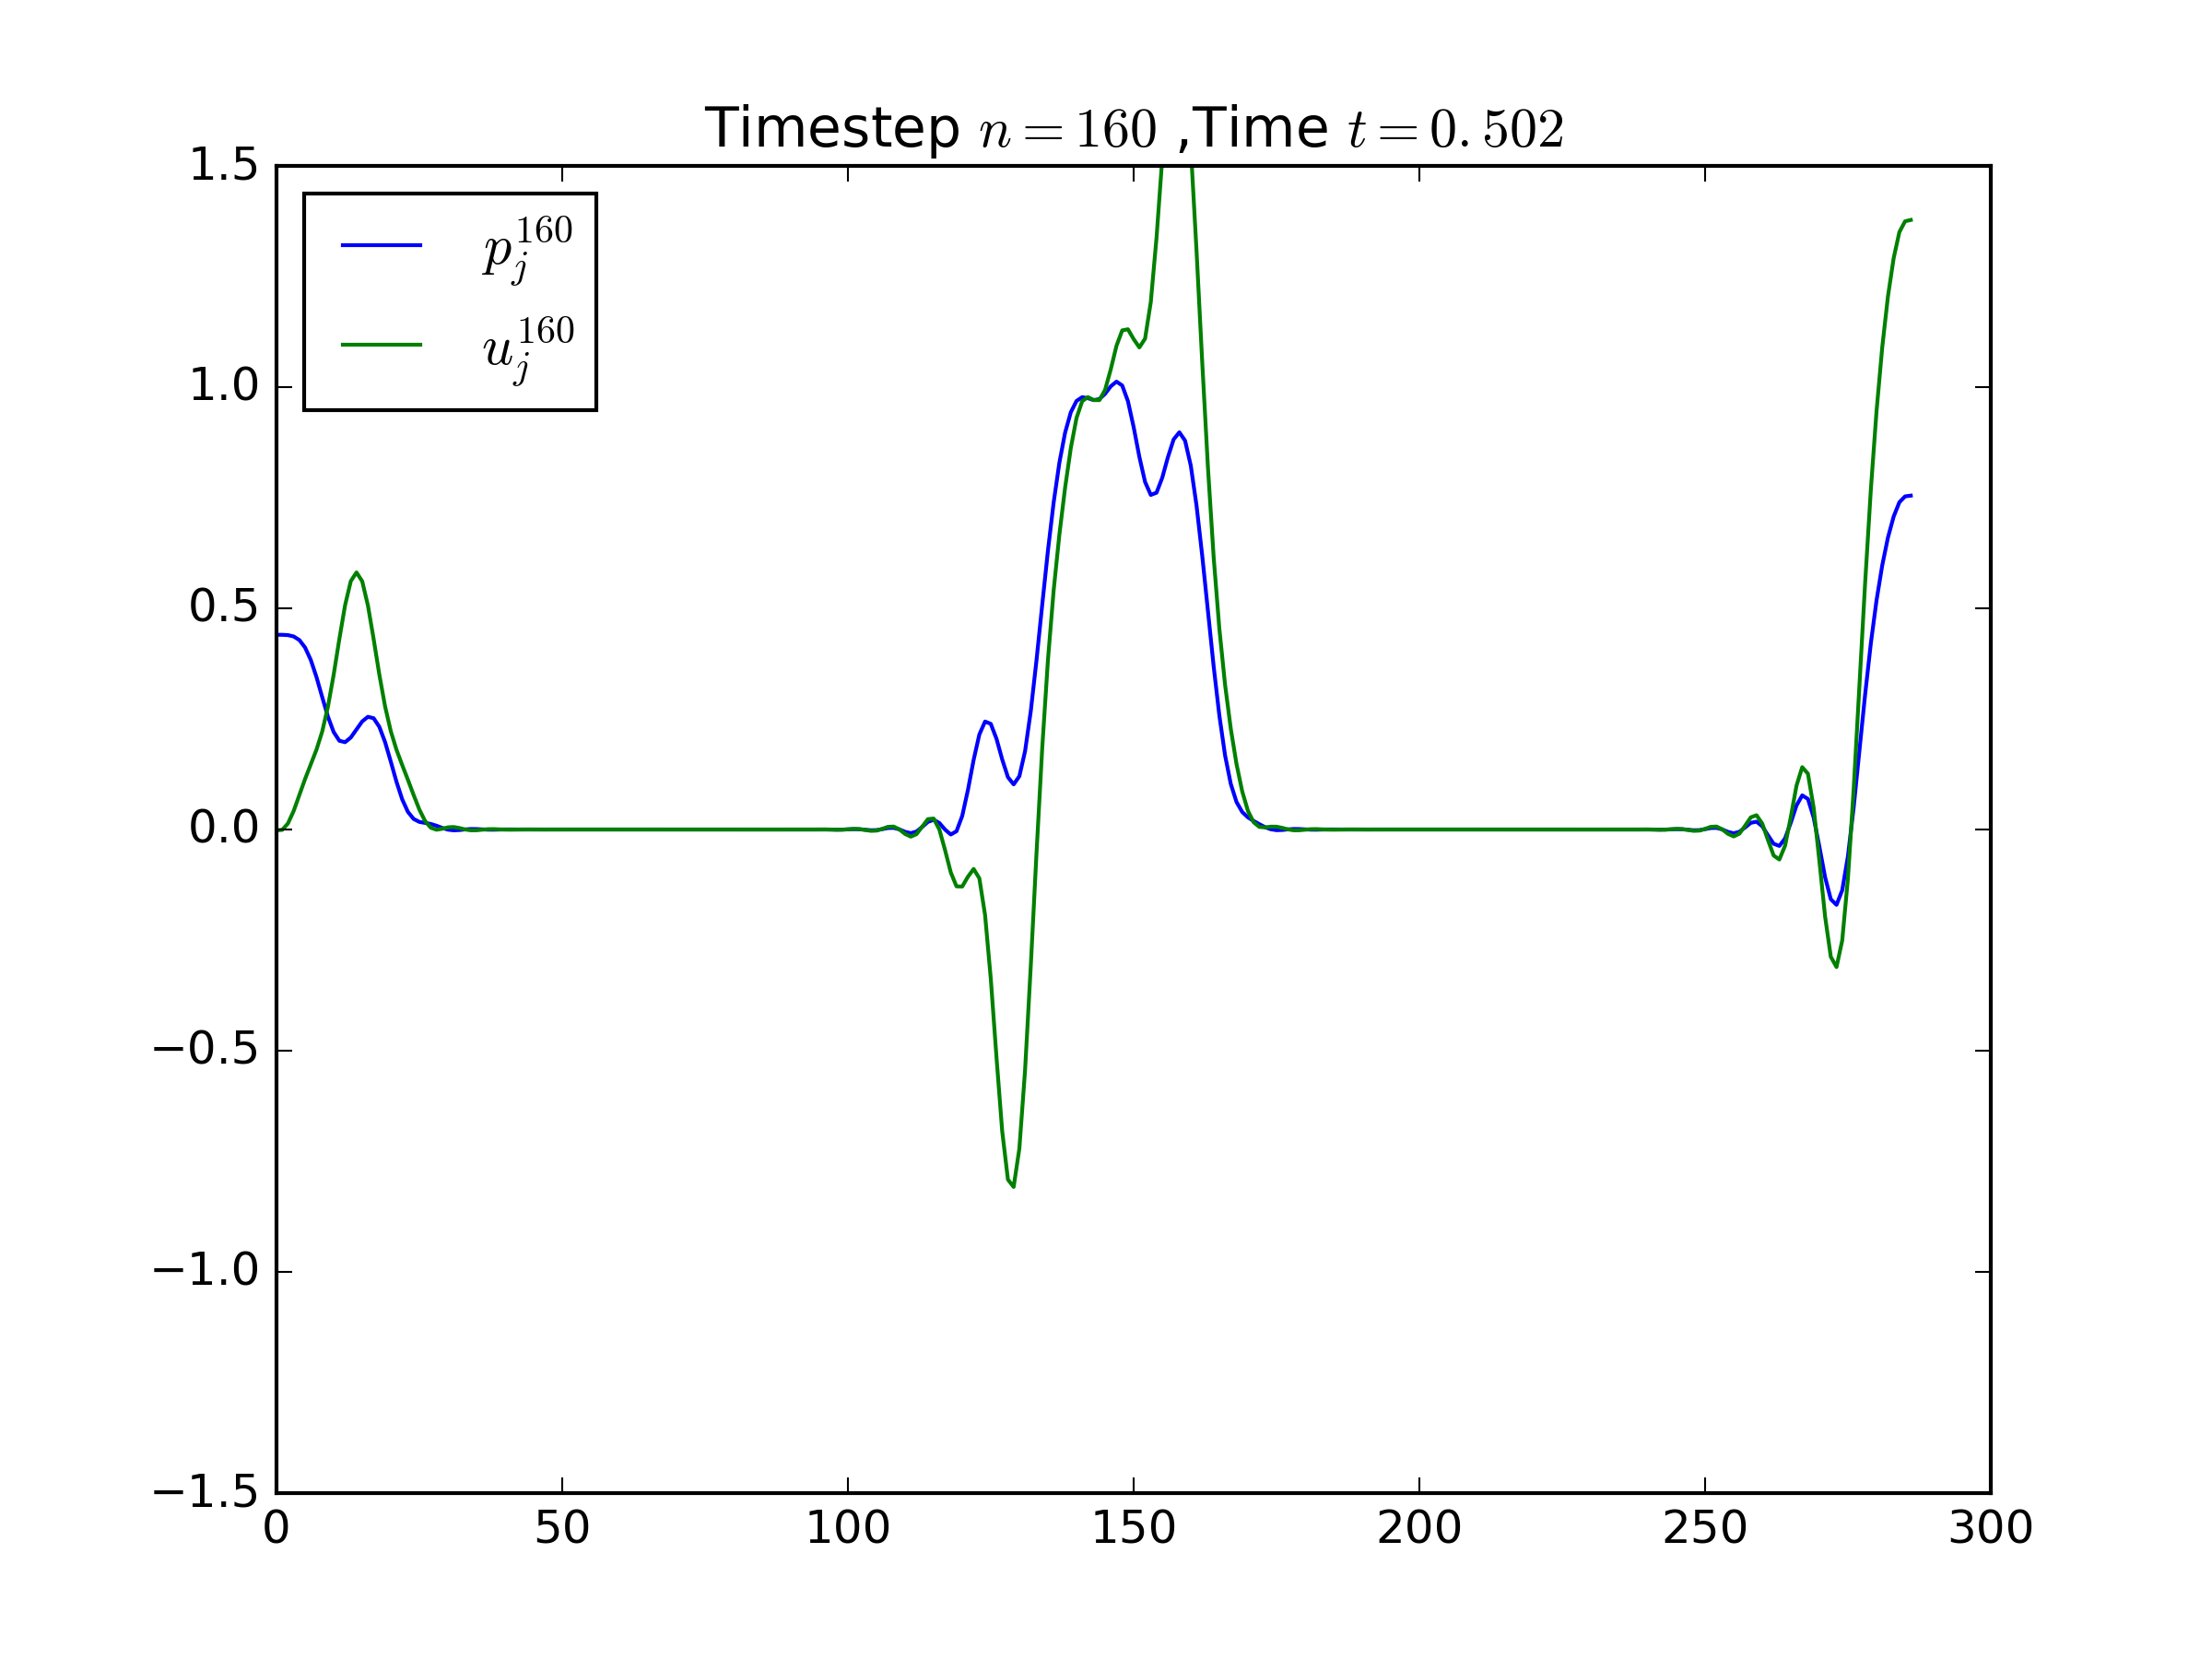
\includegraphics[width=0.31\textwidth]{figures/problem_1_b_016.png}
            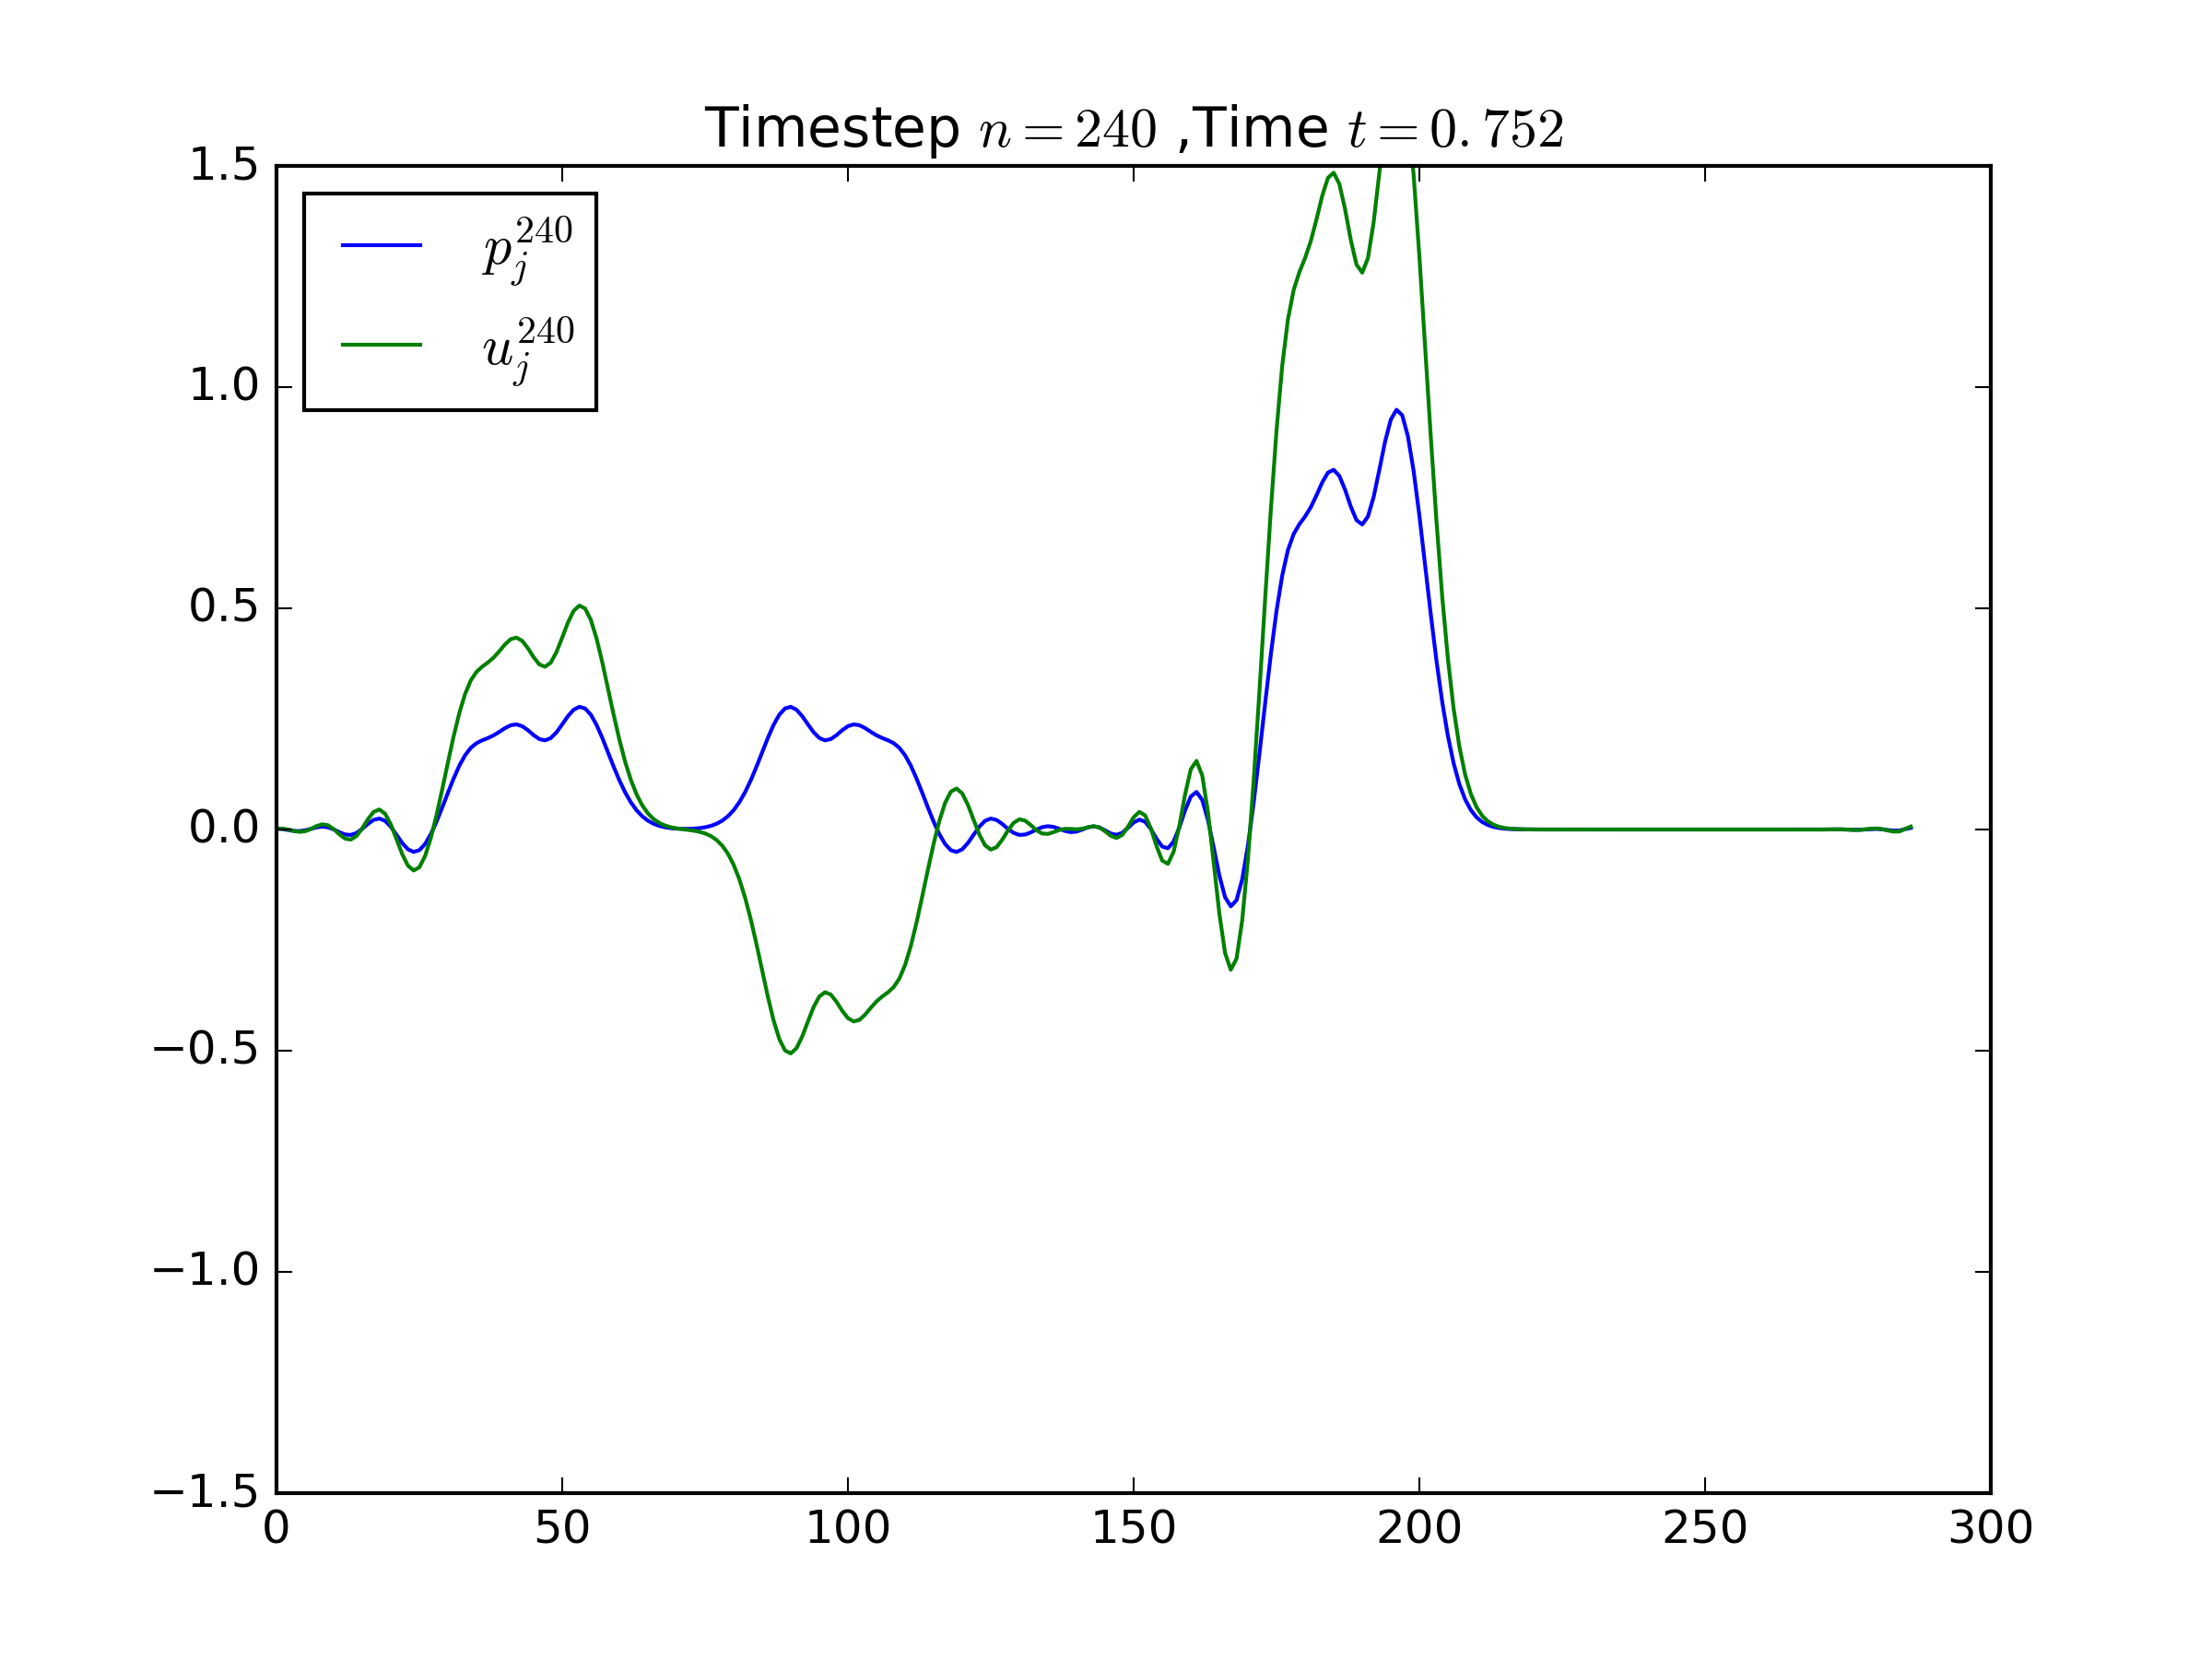
\includegraphics[width=0.31\textwidth]{figures/problem_1_b_024.png}
            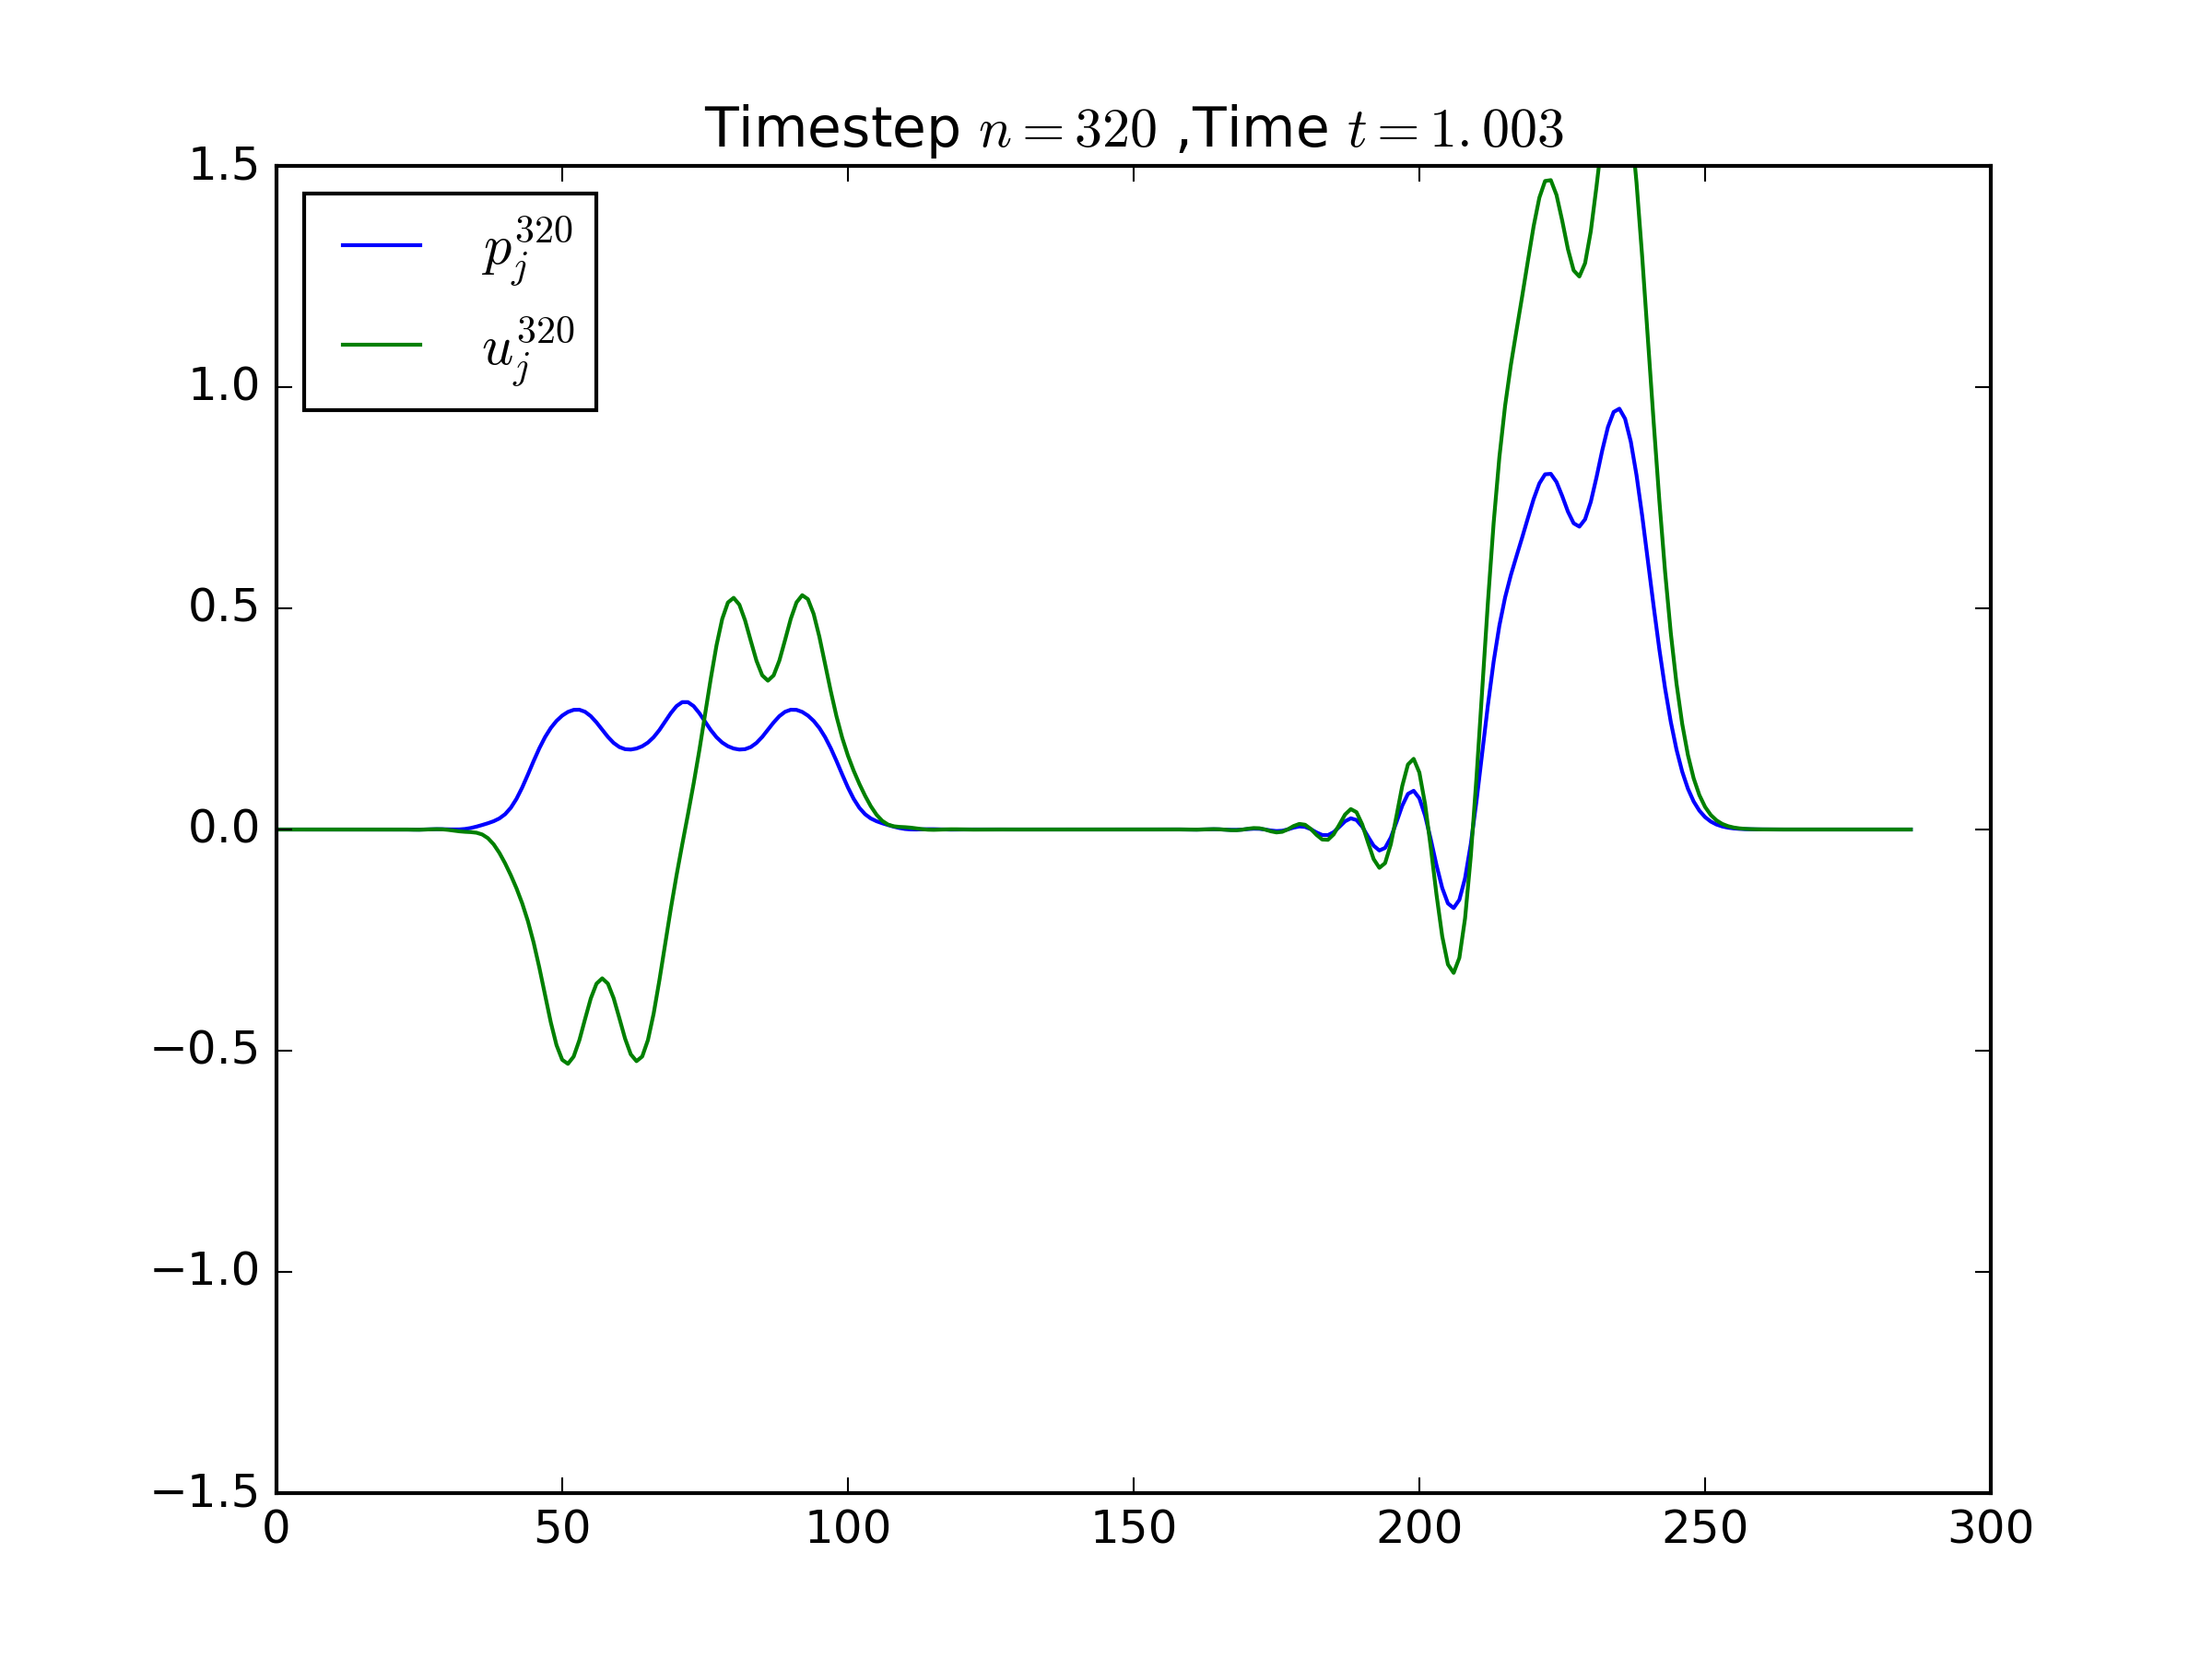
\includegraphics[width=0.31\textwidth]{figures/problem_1_b_032.png}
            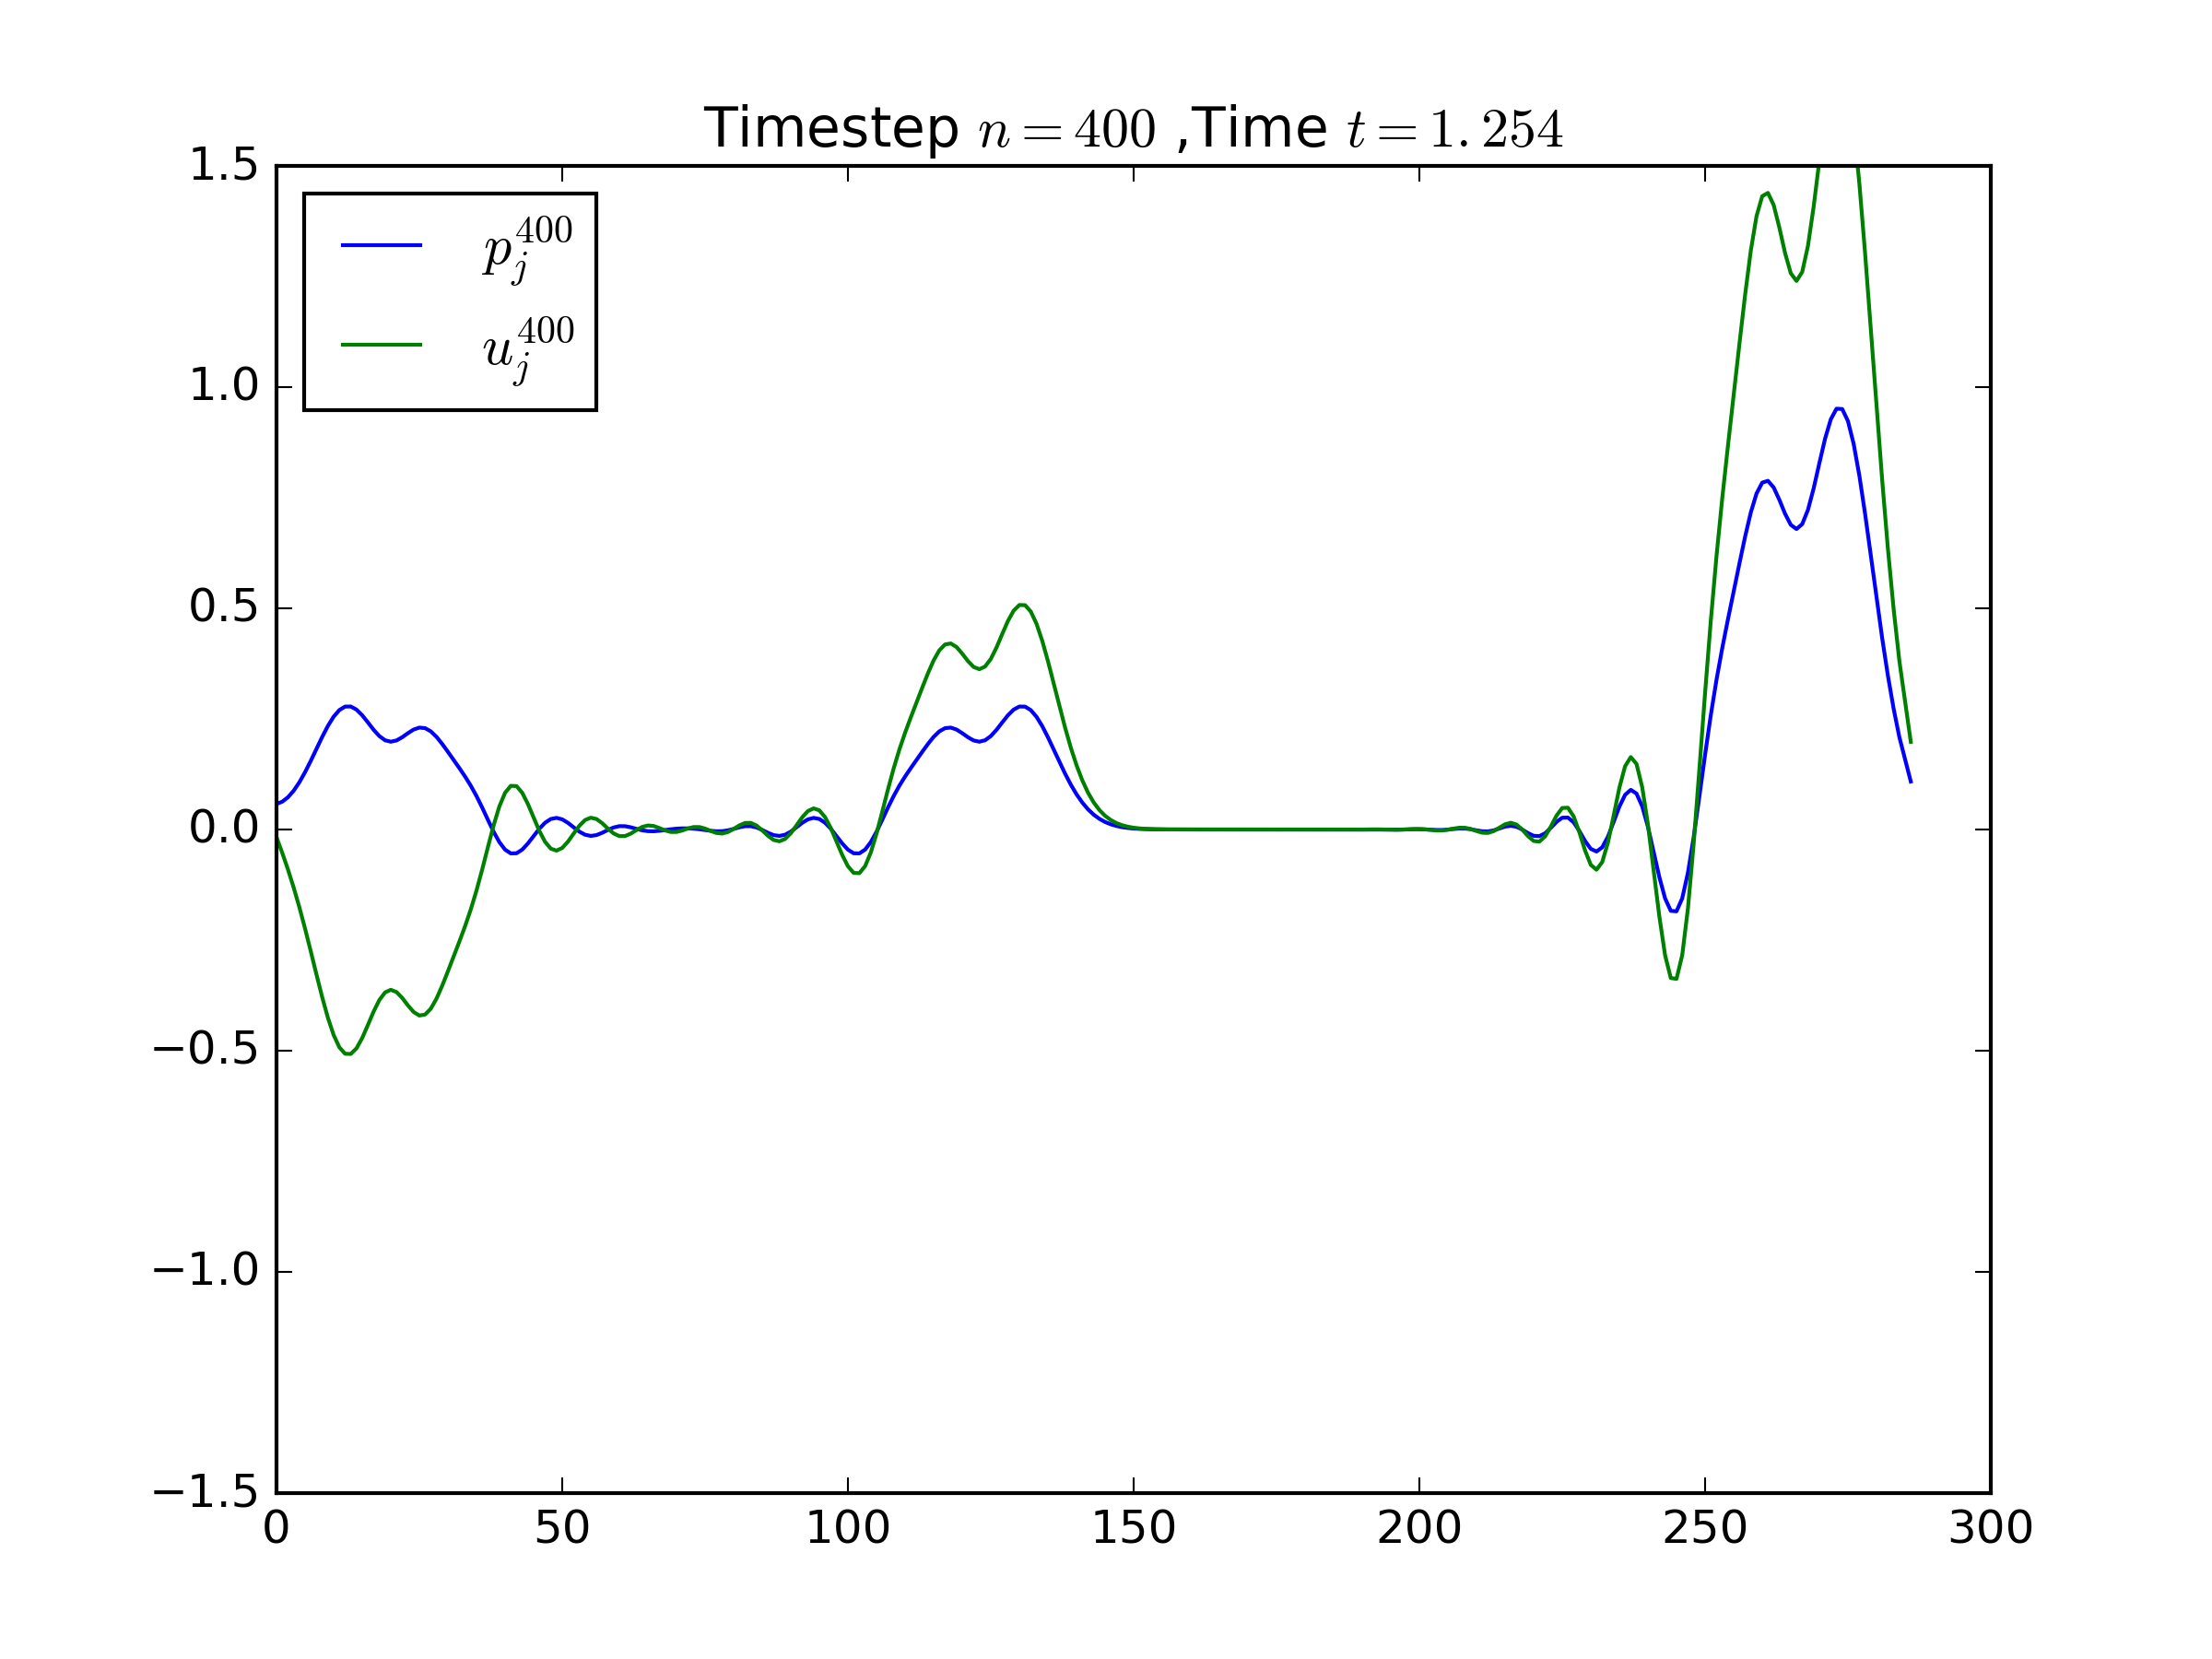
\includegraphics[width=0.31\textwidth]{figures/problem_1_b_040.png}
            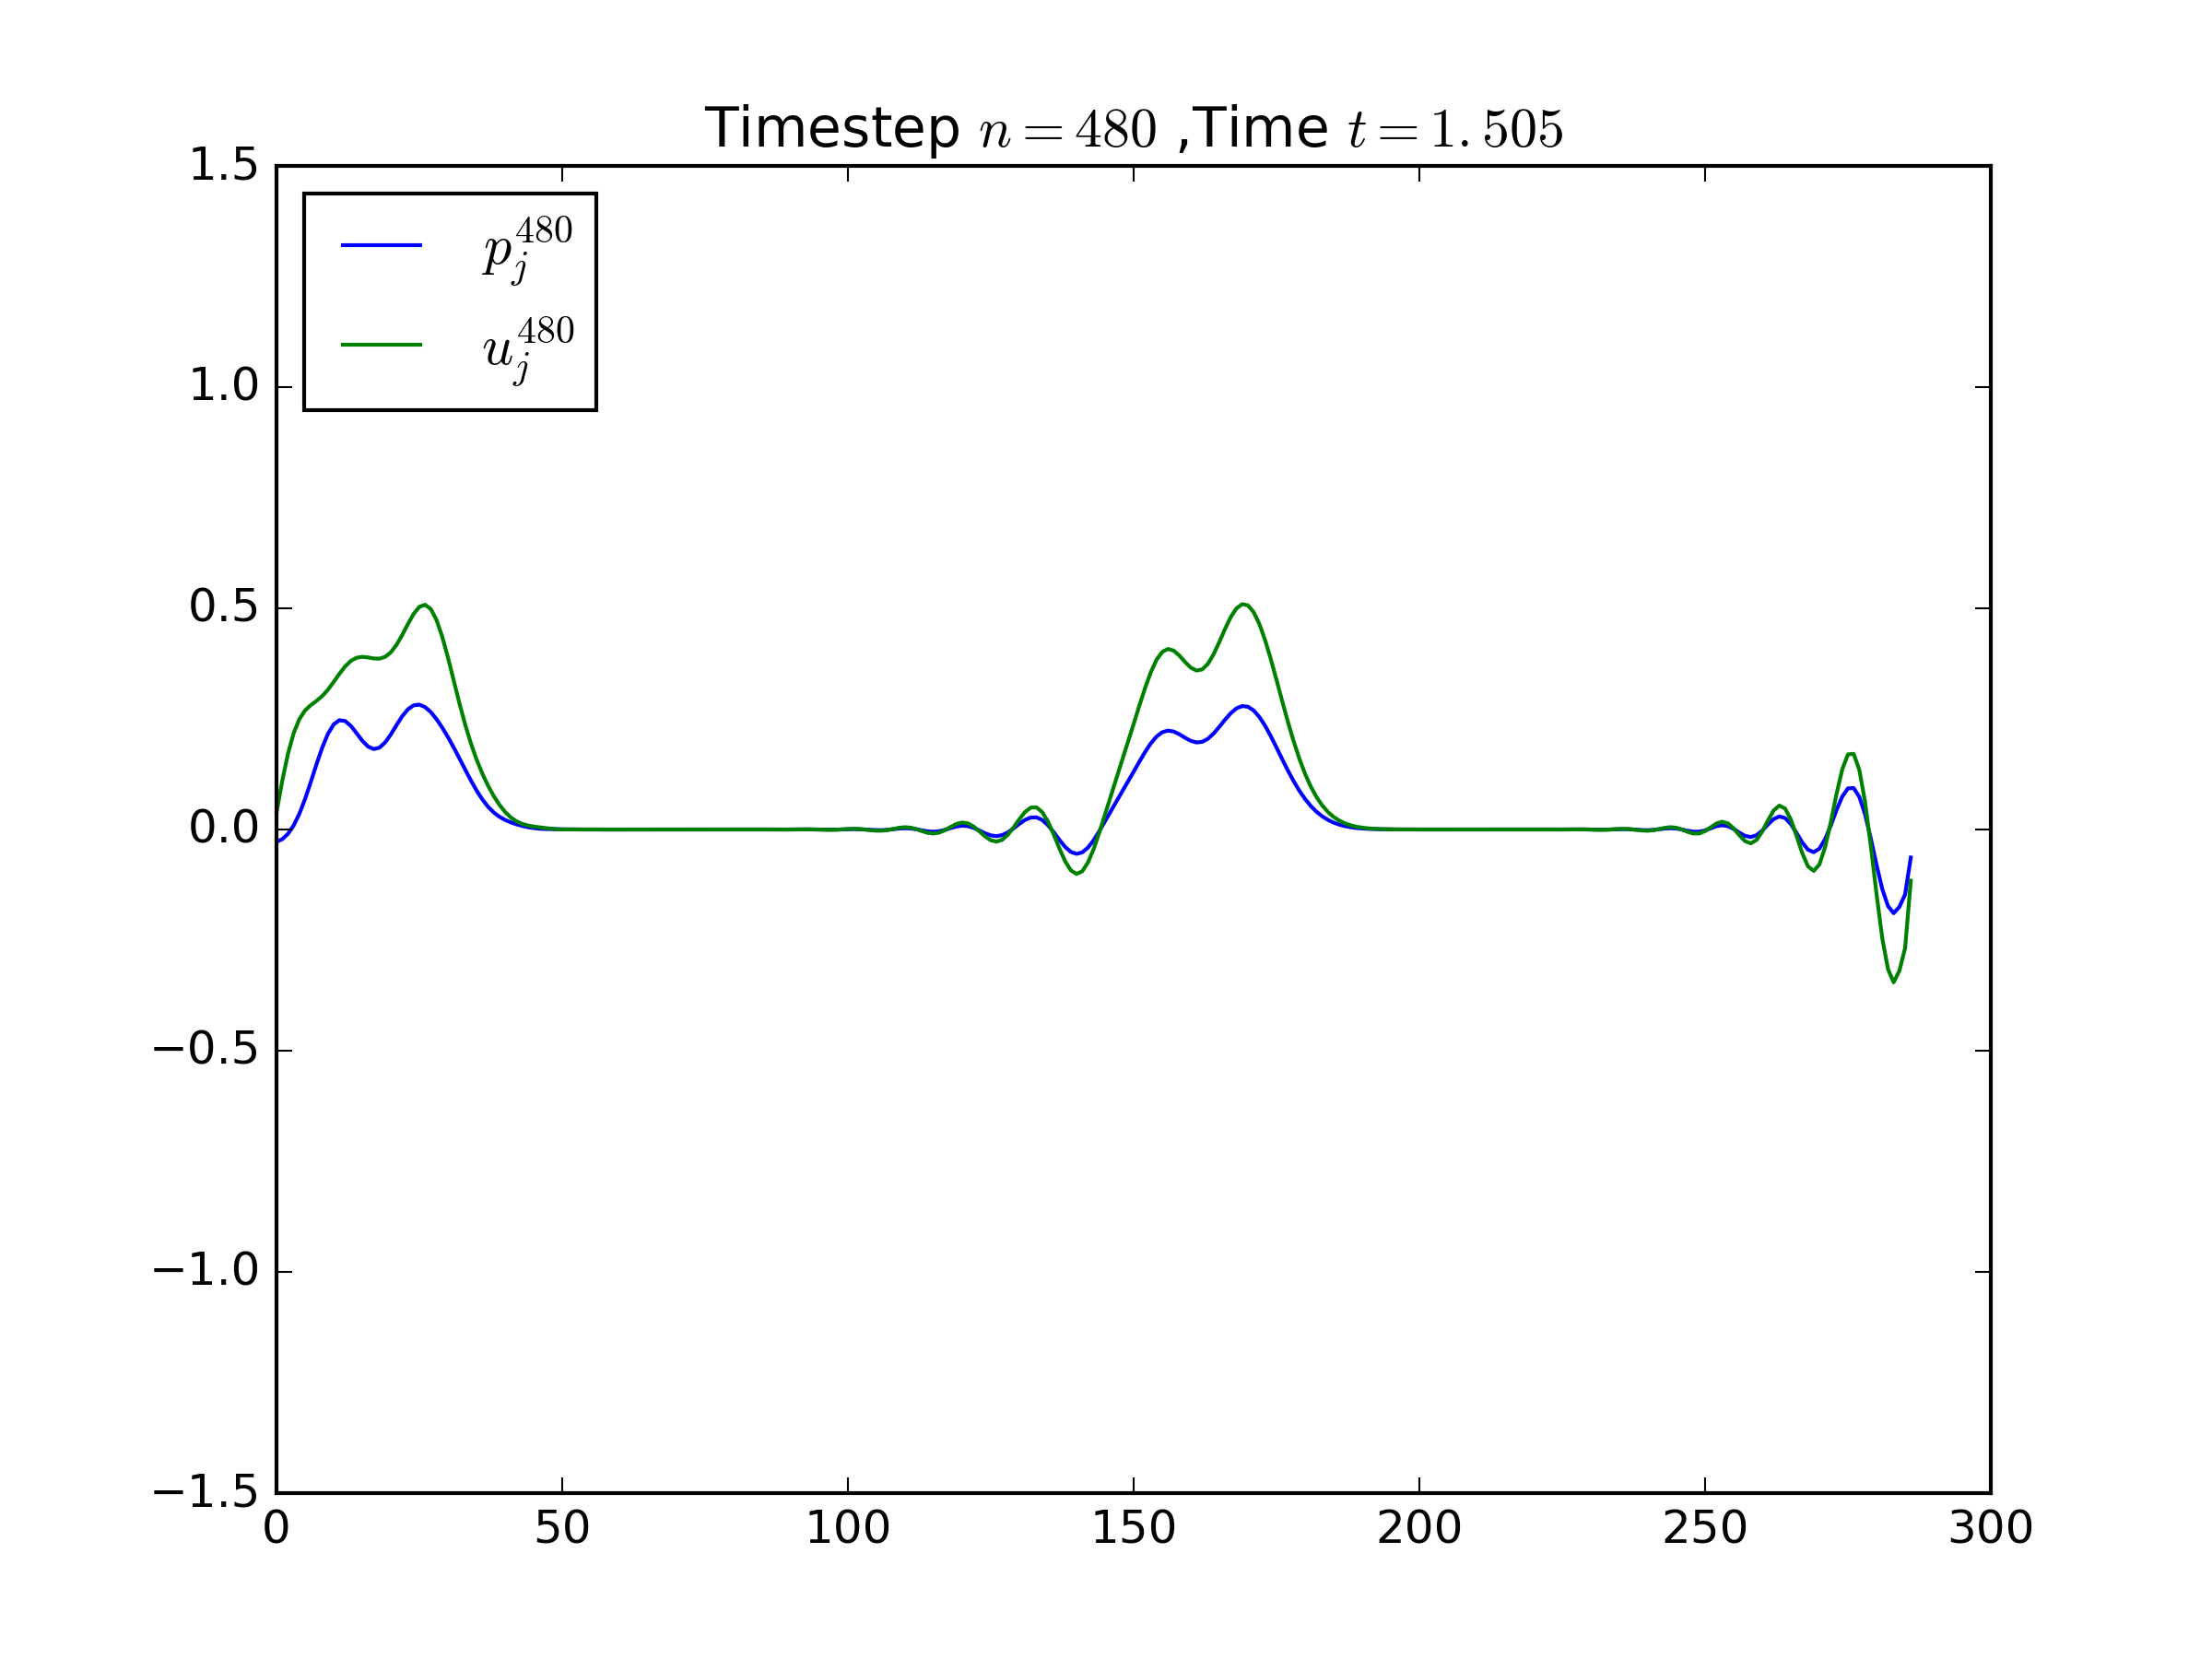
\includegraphics[width=0.31\textwidth]{figures/problem_1_b_048.png}
            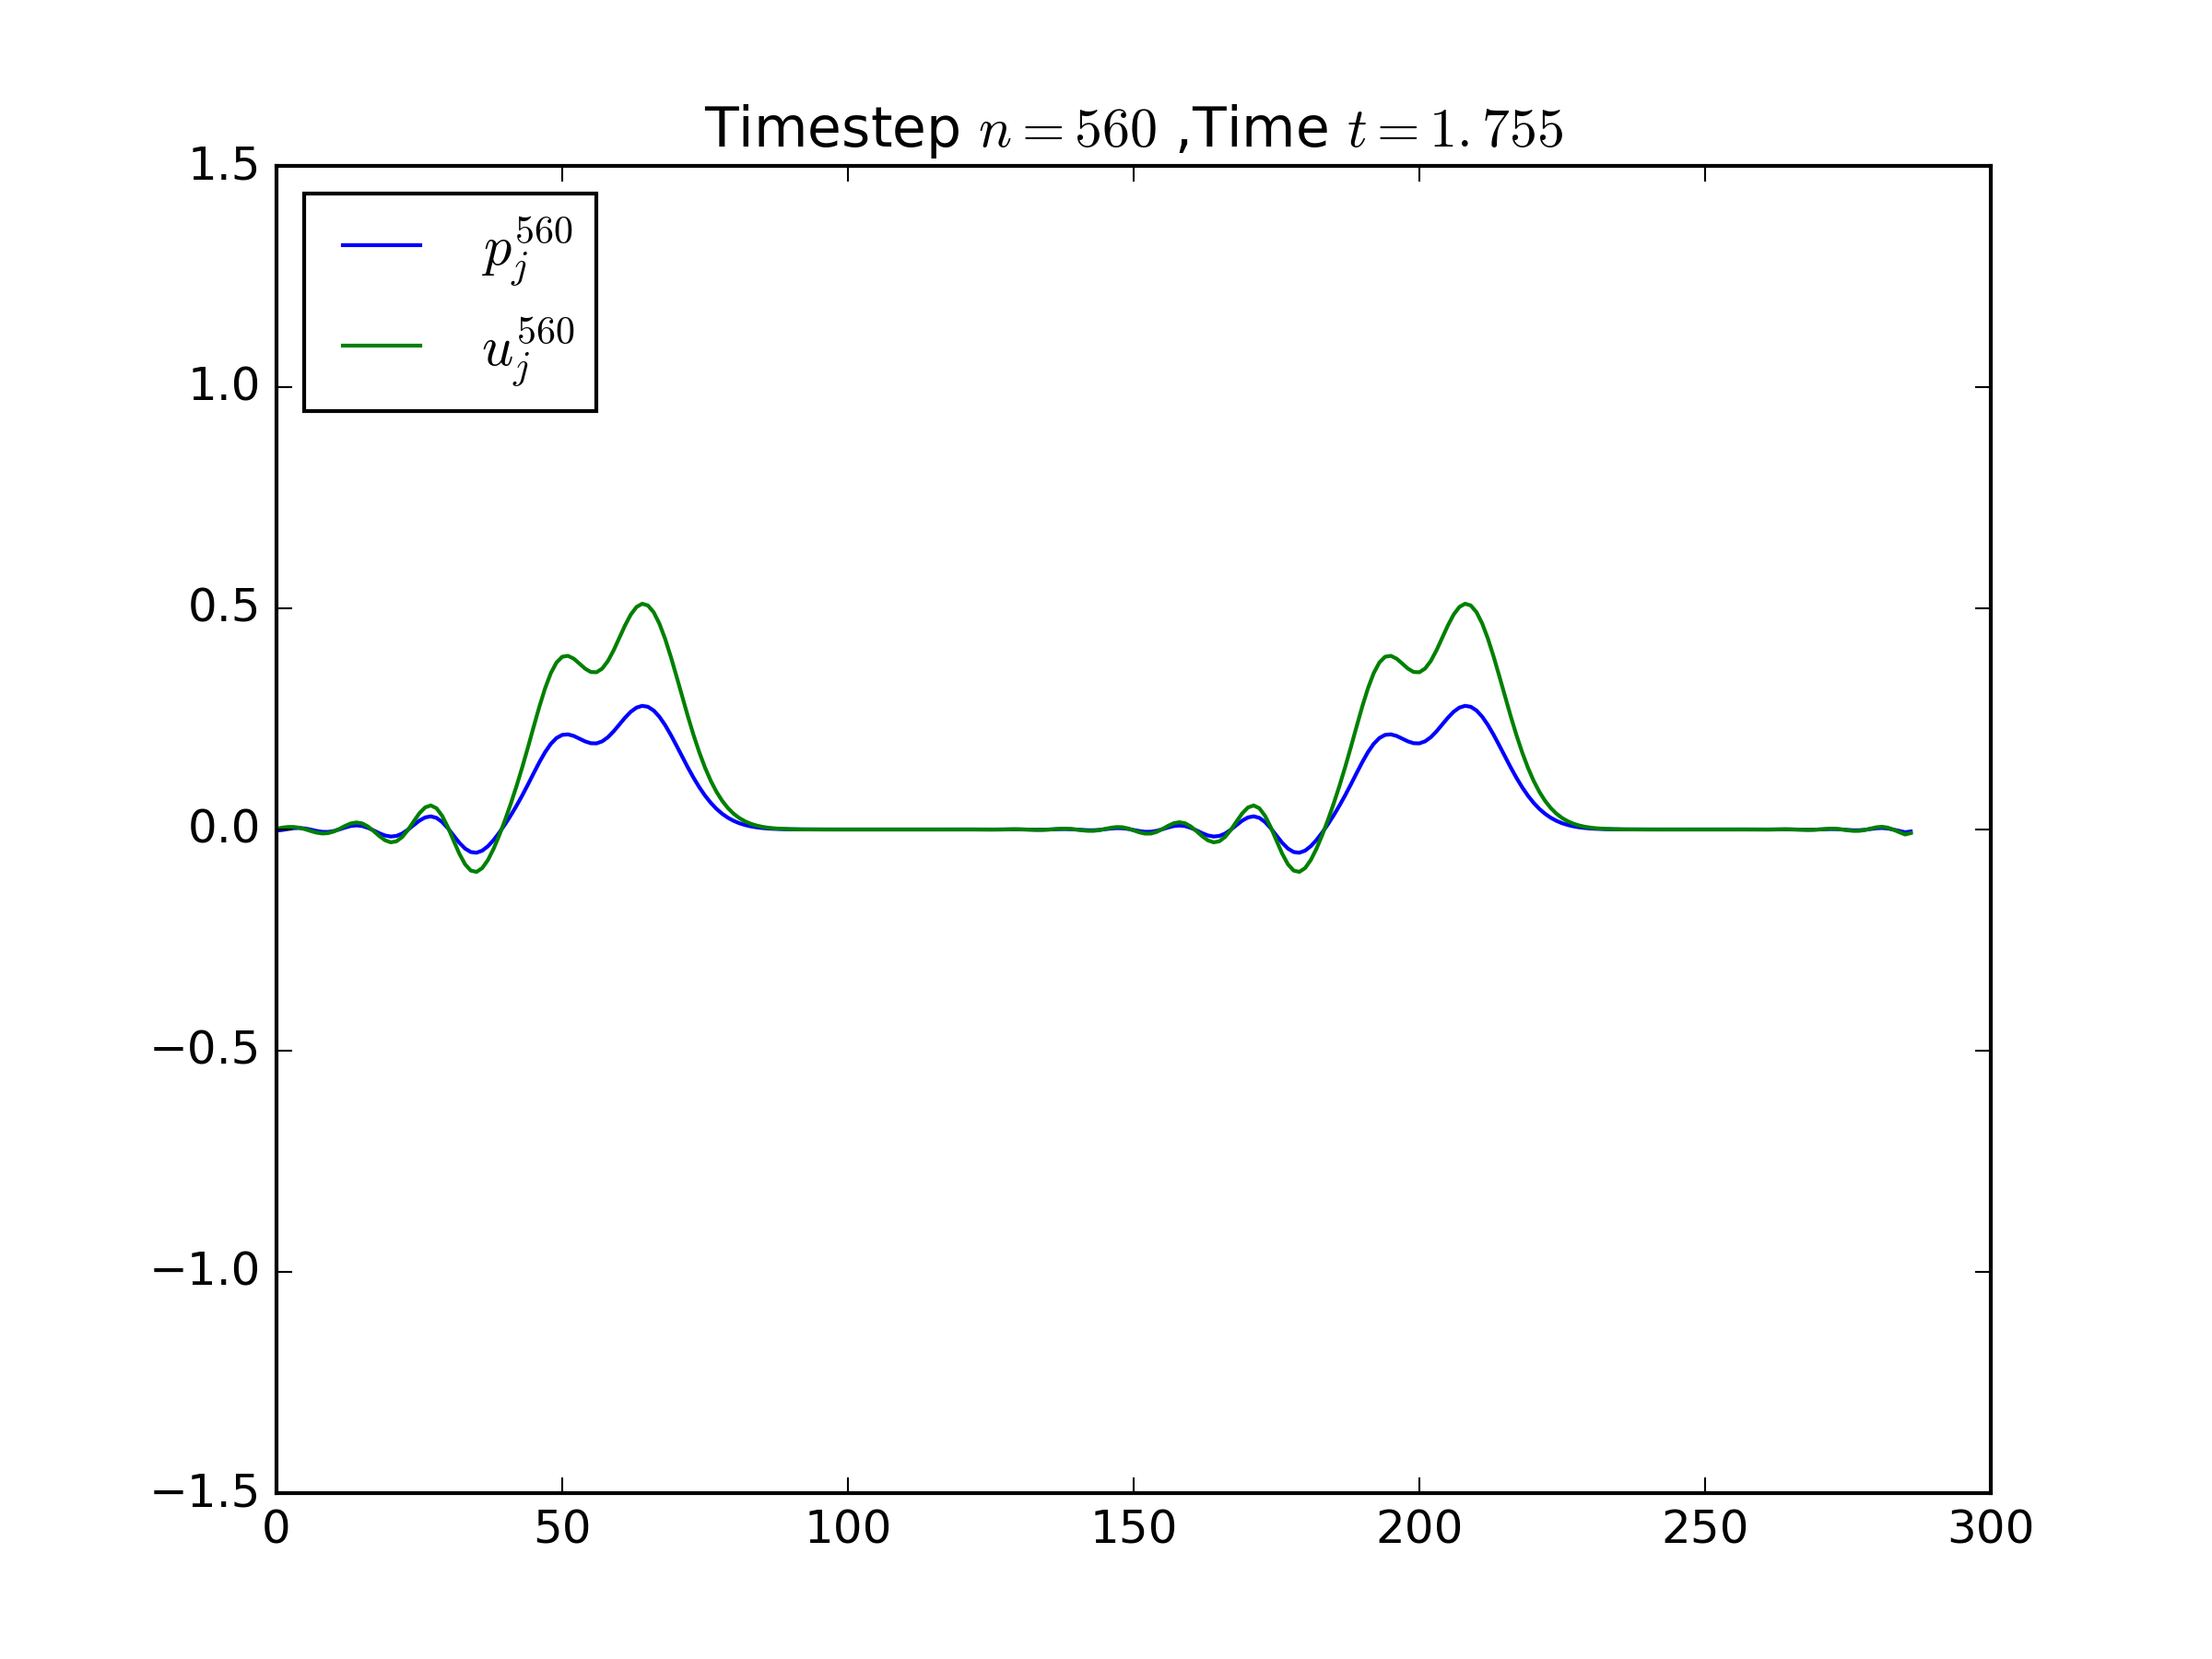
\includegraphics[width=0.31\textwidth]{figures/problem_1_b_056.png}
            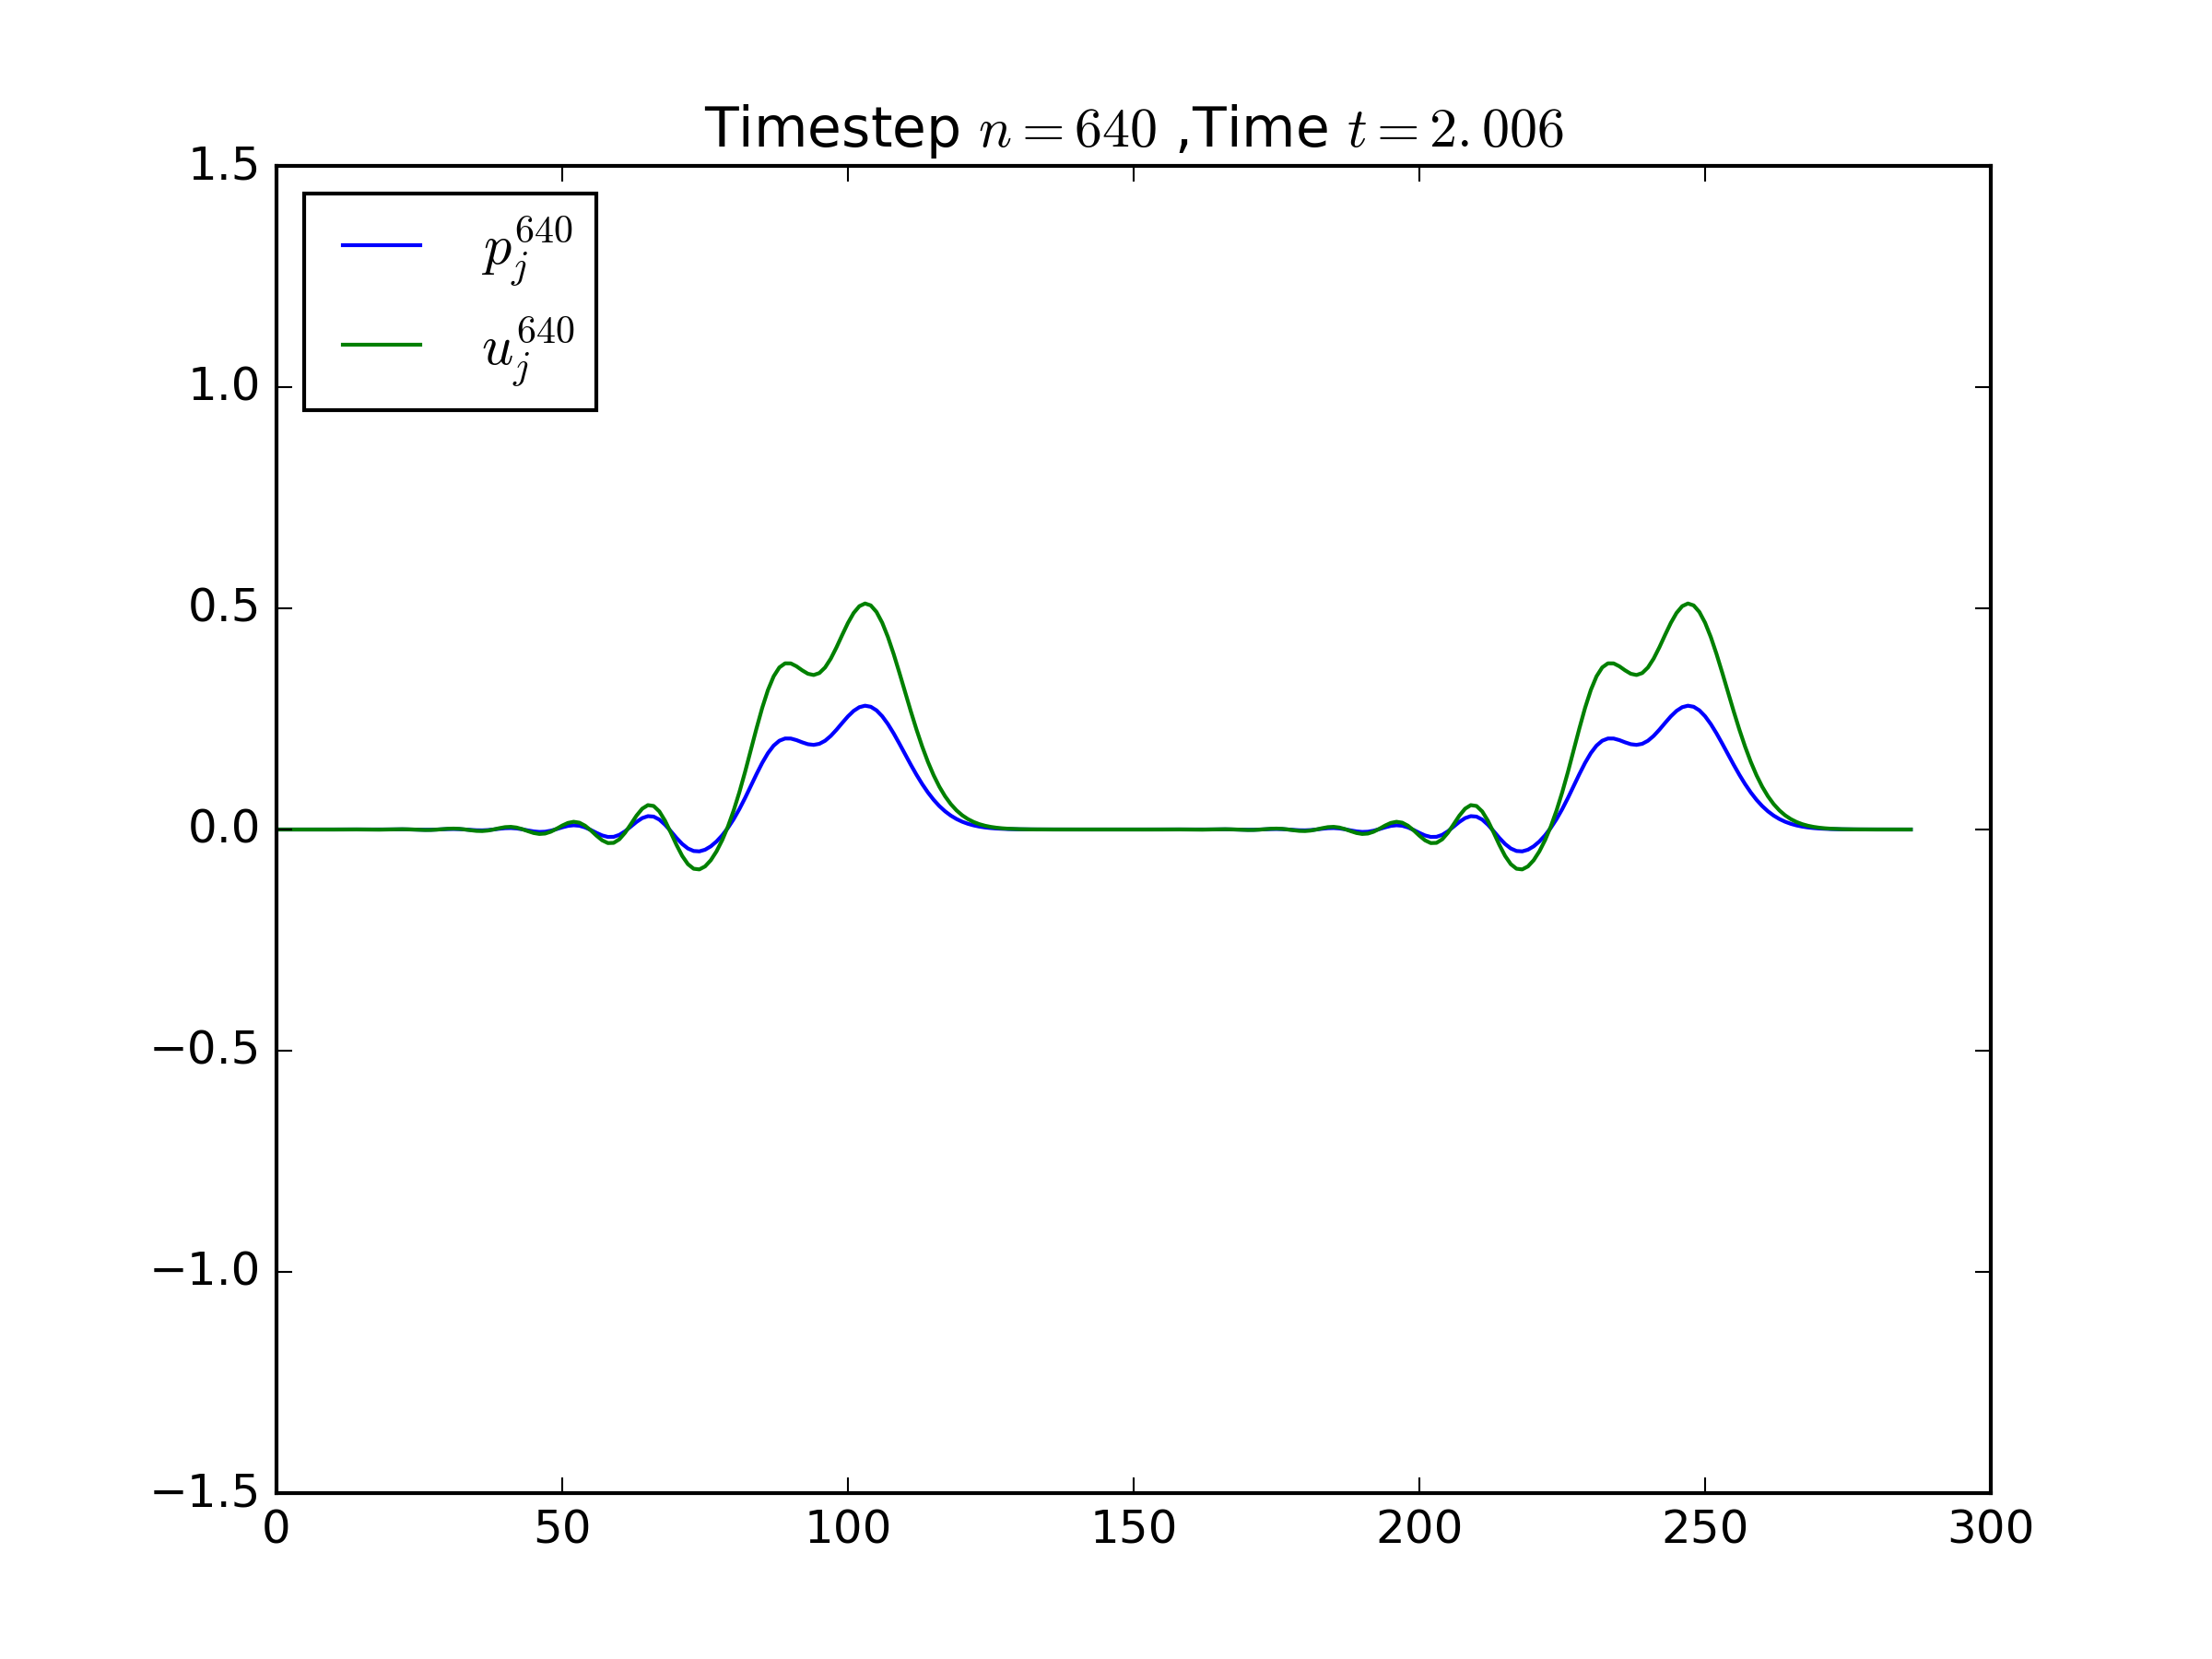
\includegraphics[width=0.31\textwidth]{figures/problem_1_b_064.png}
            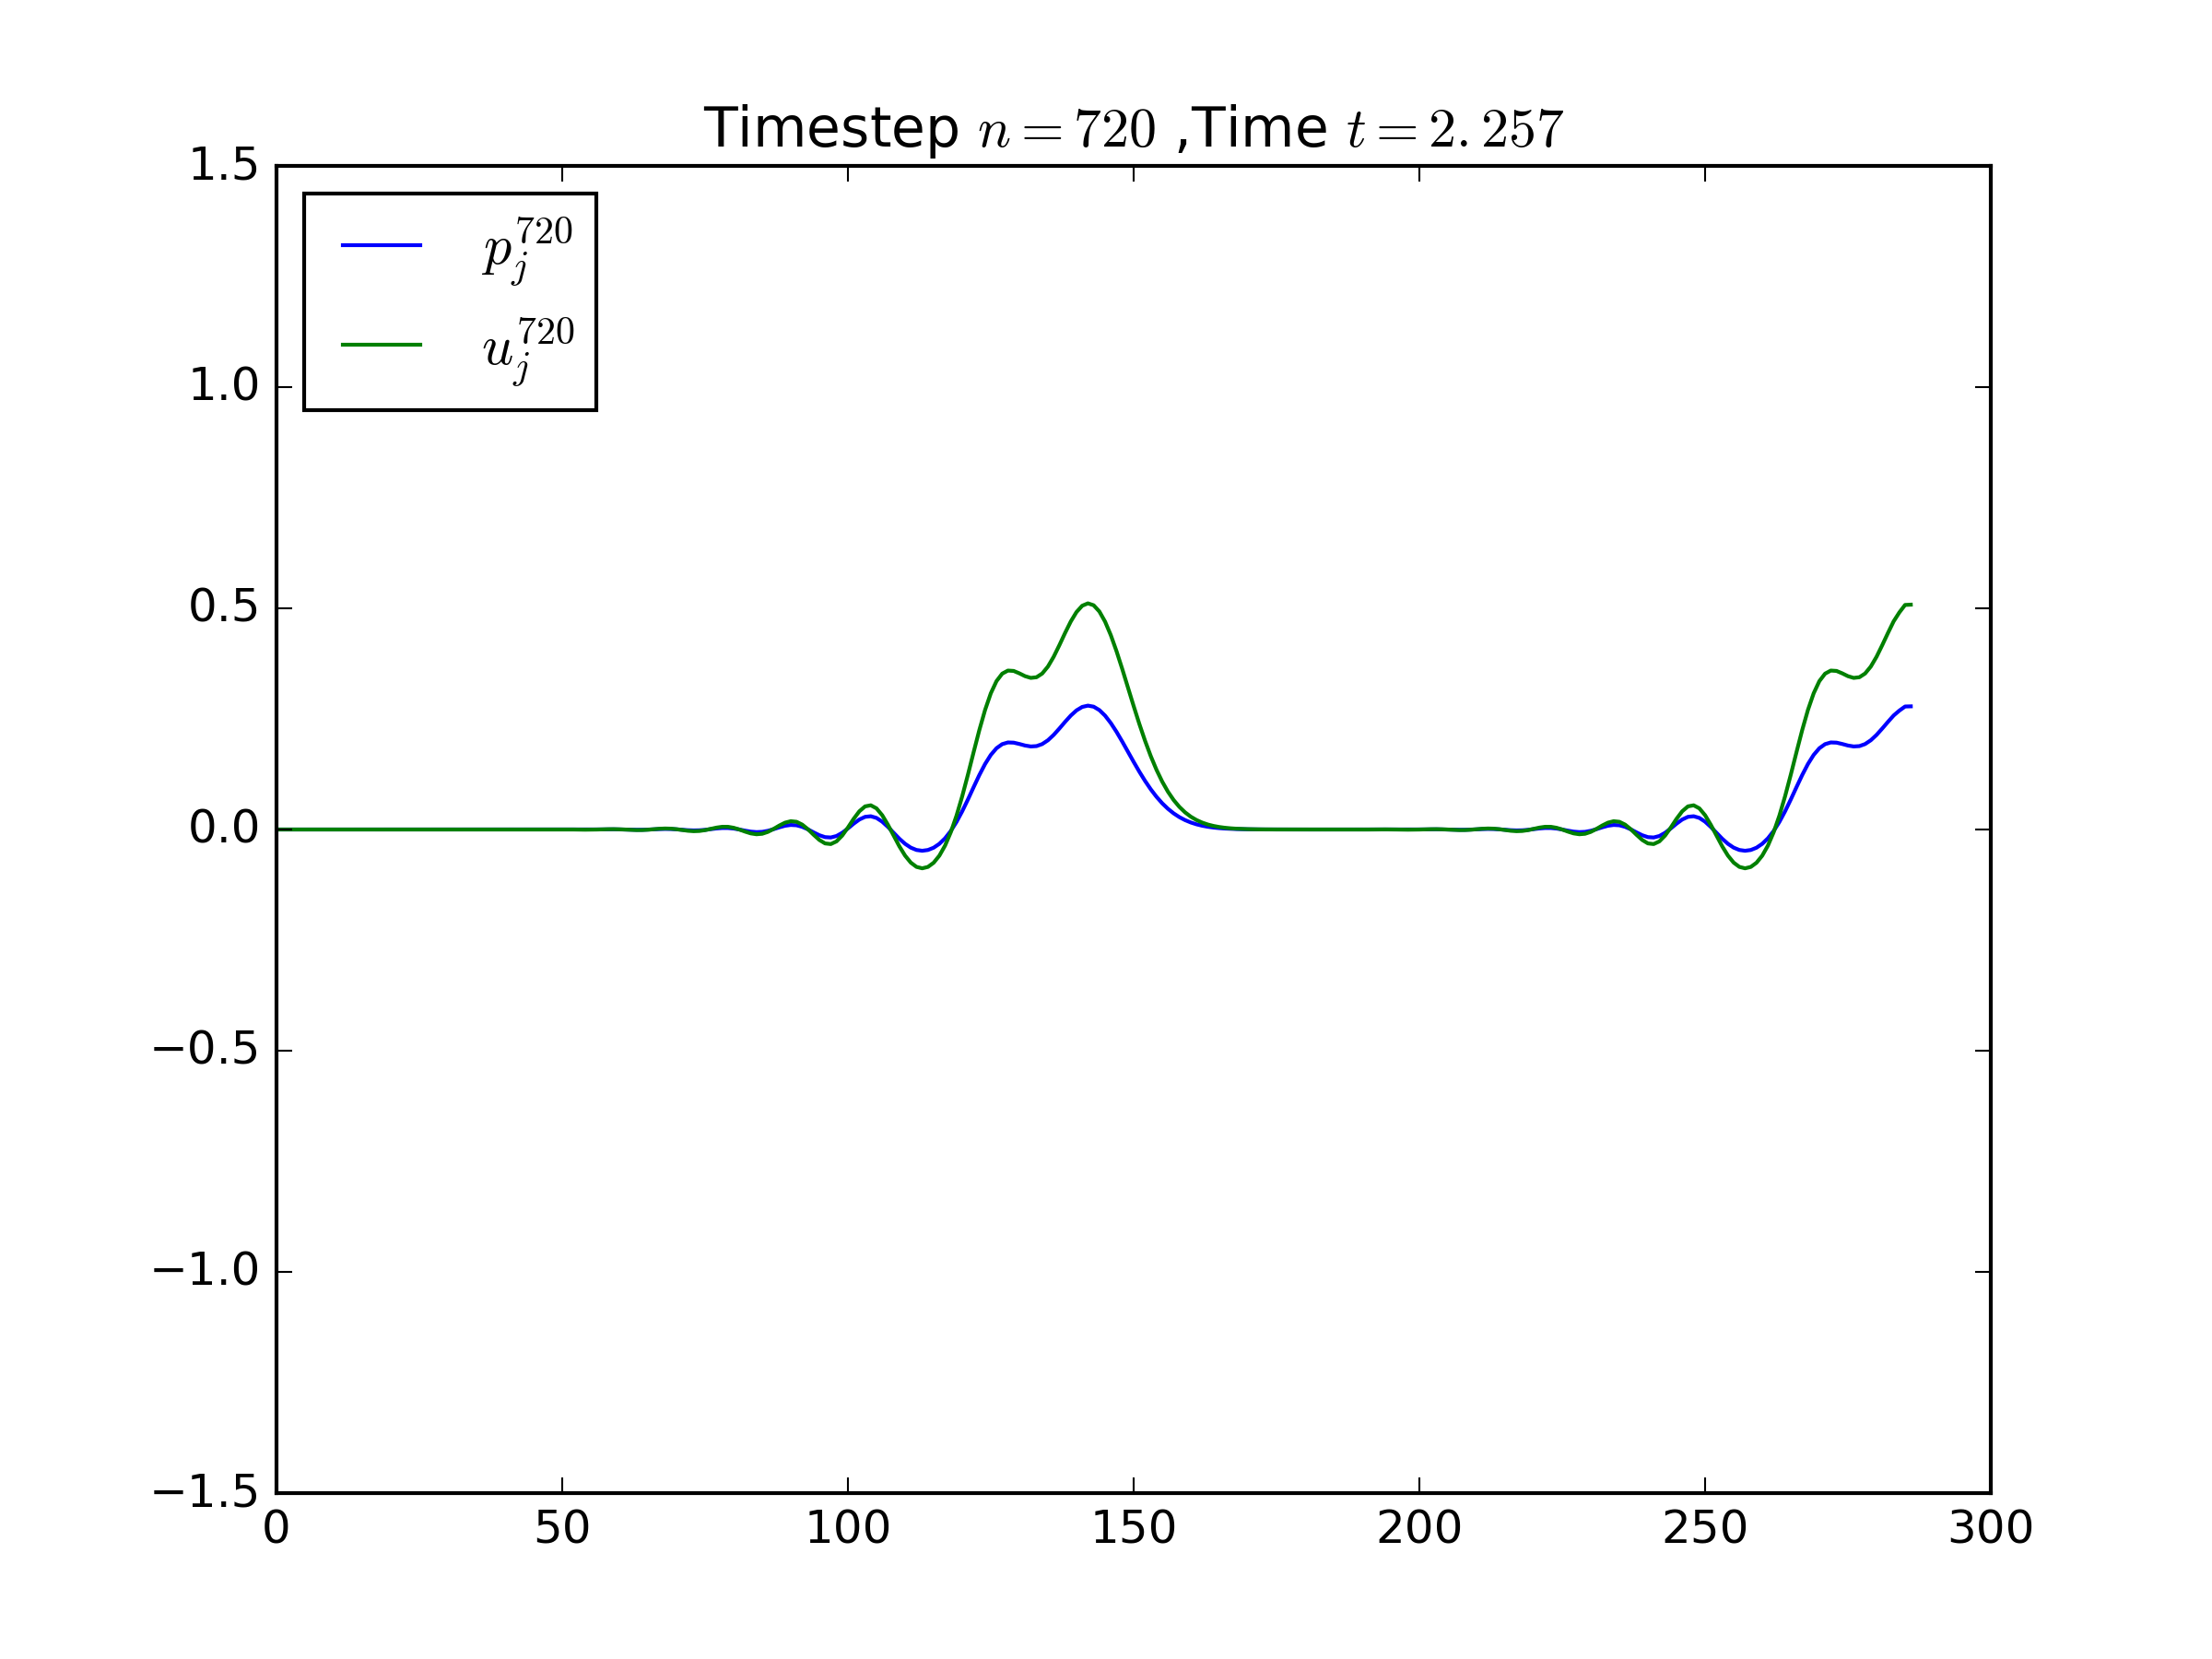
\includegraphics[width=0.31\textwidth]{figures/problem_1_b_072.png}
            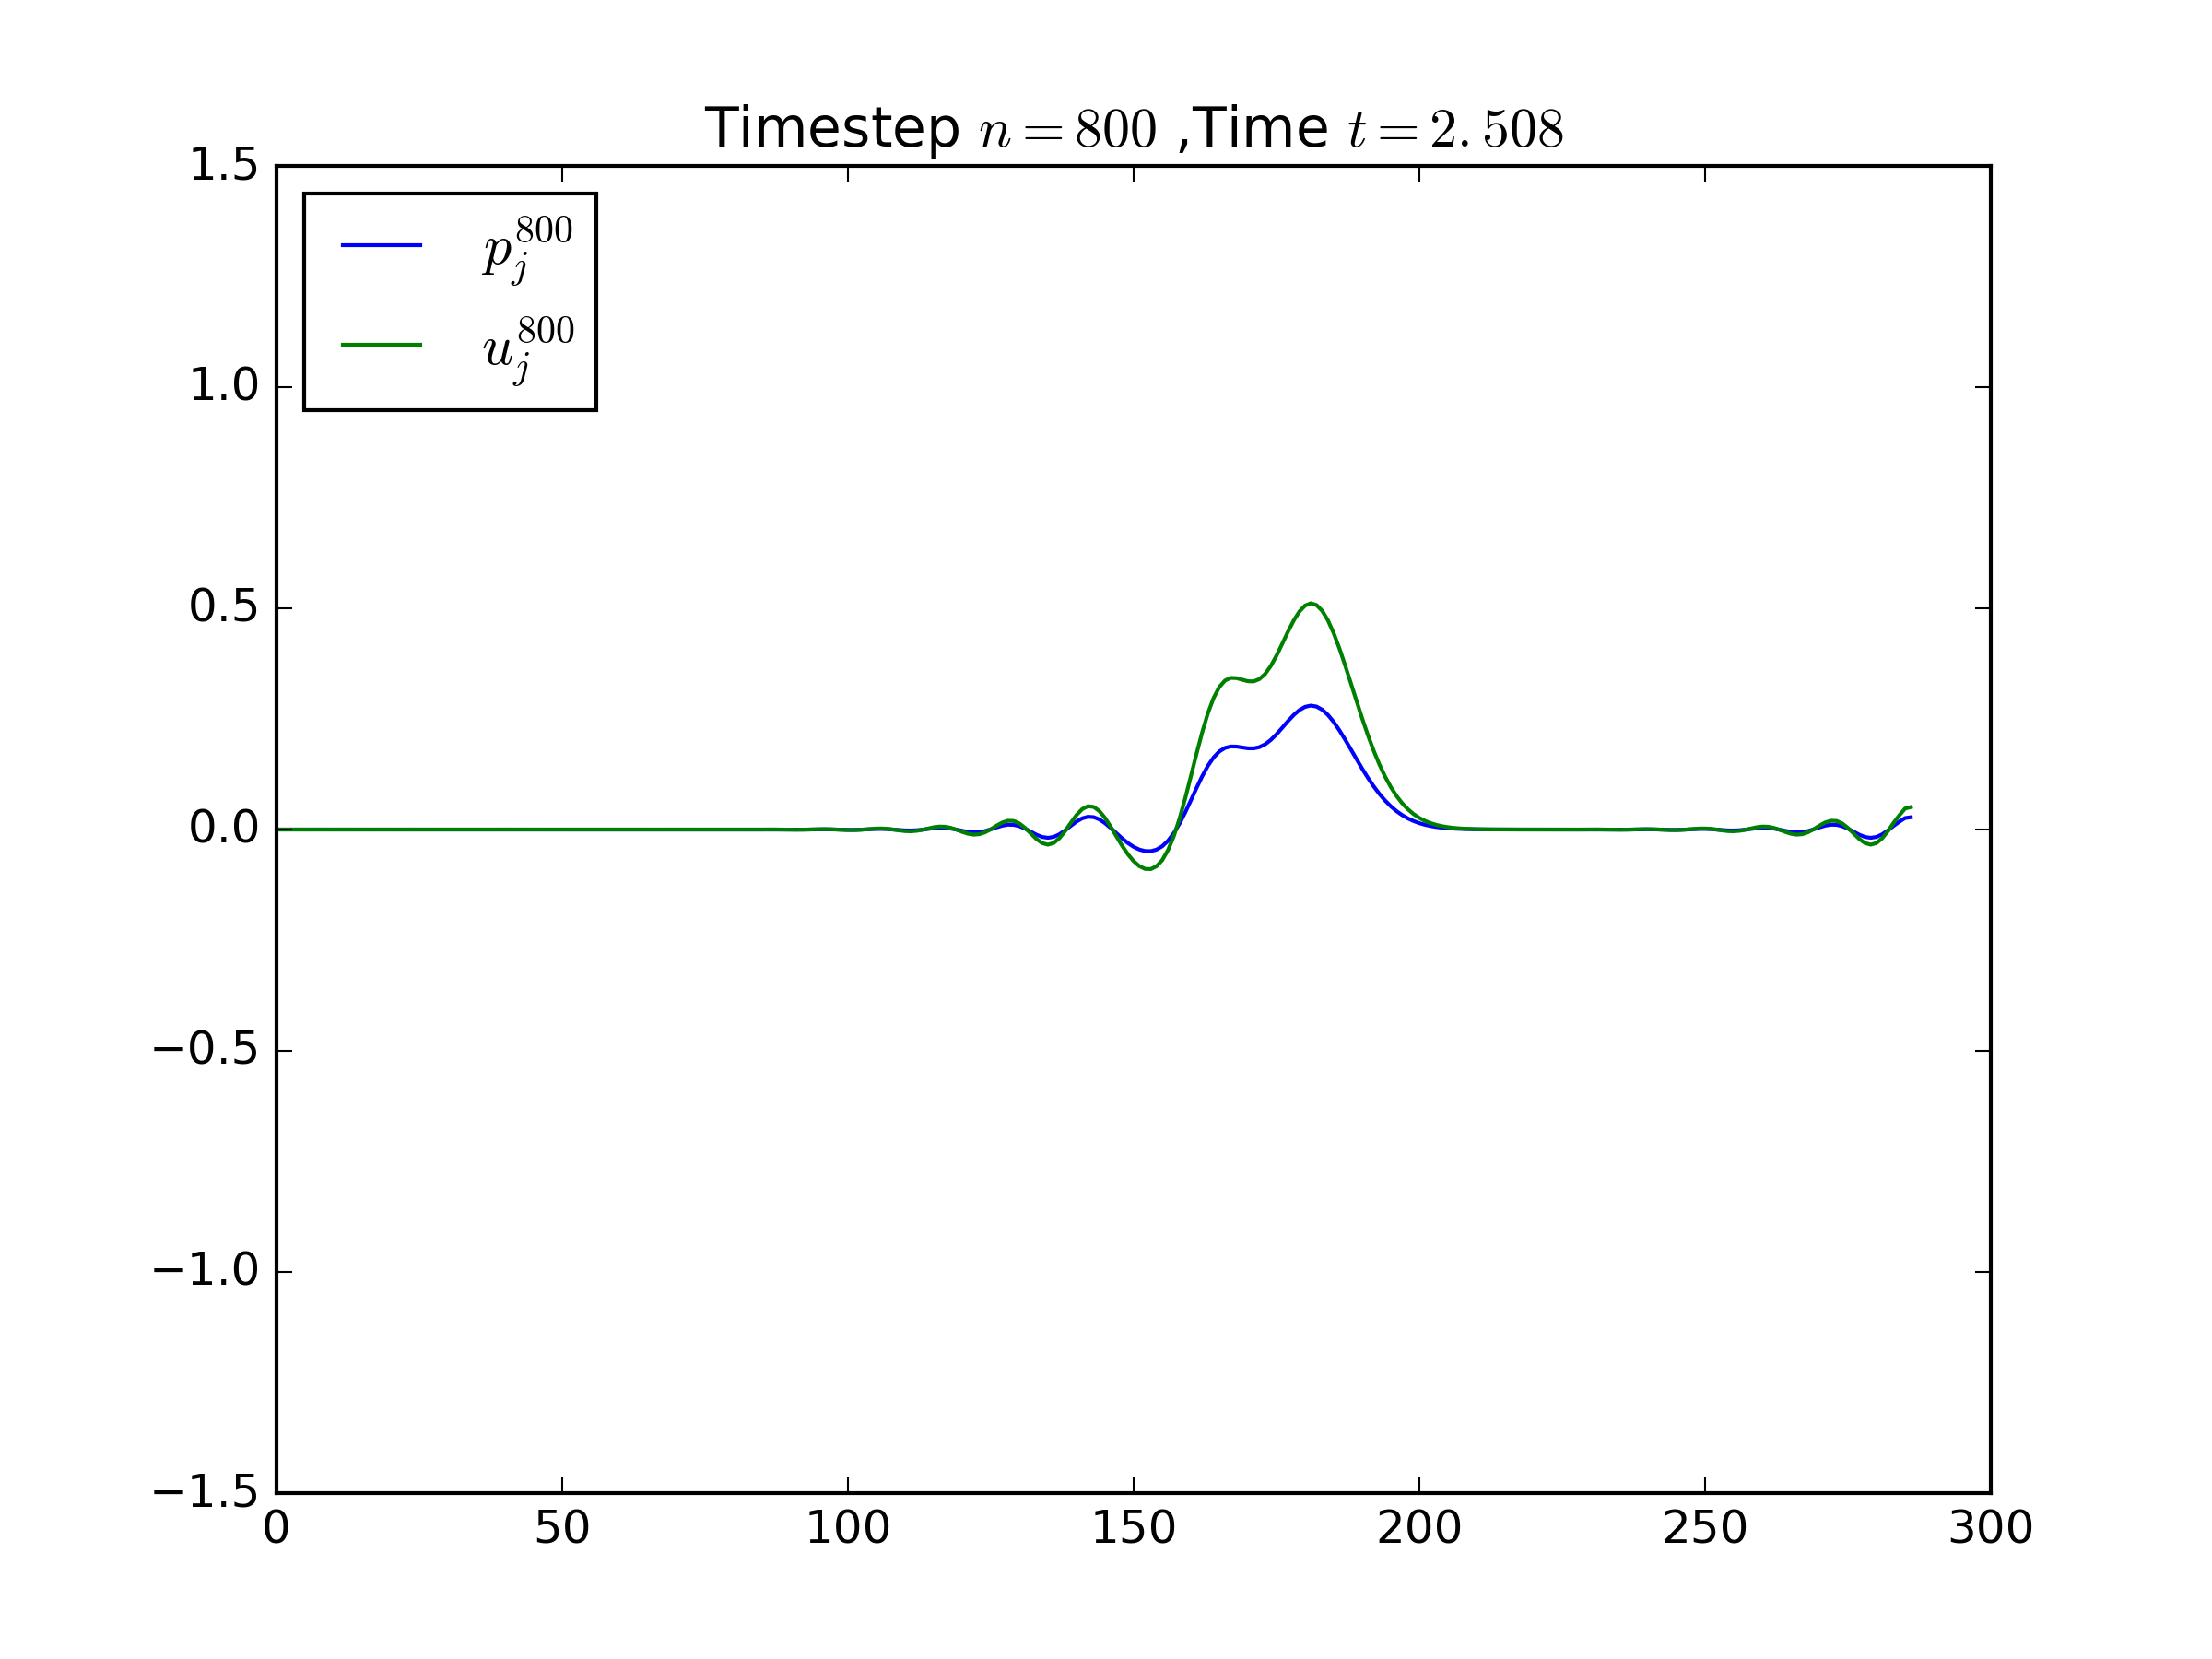
\includegraphics[width=0.31\textwidth]{figures/problem_1_b_080.png}
            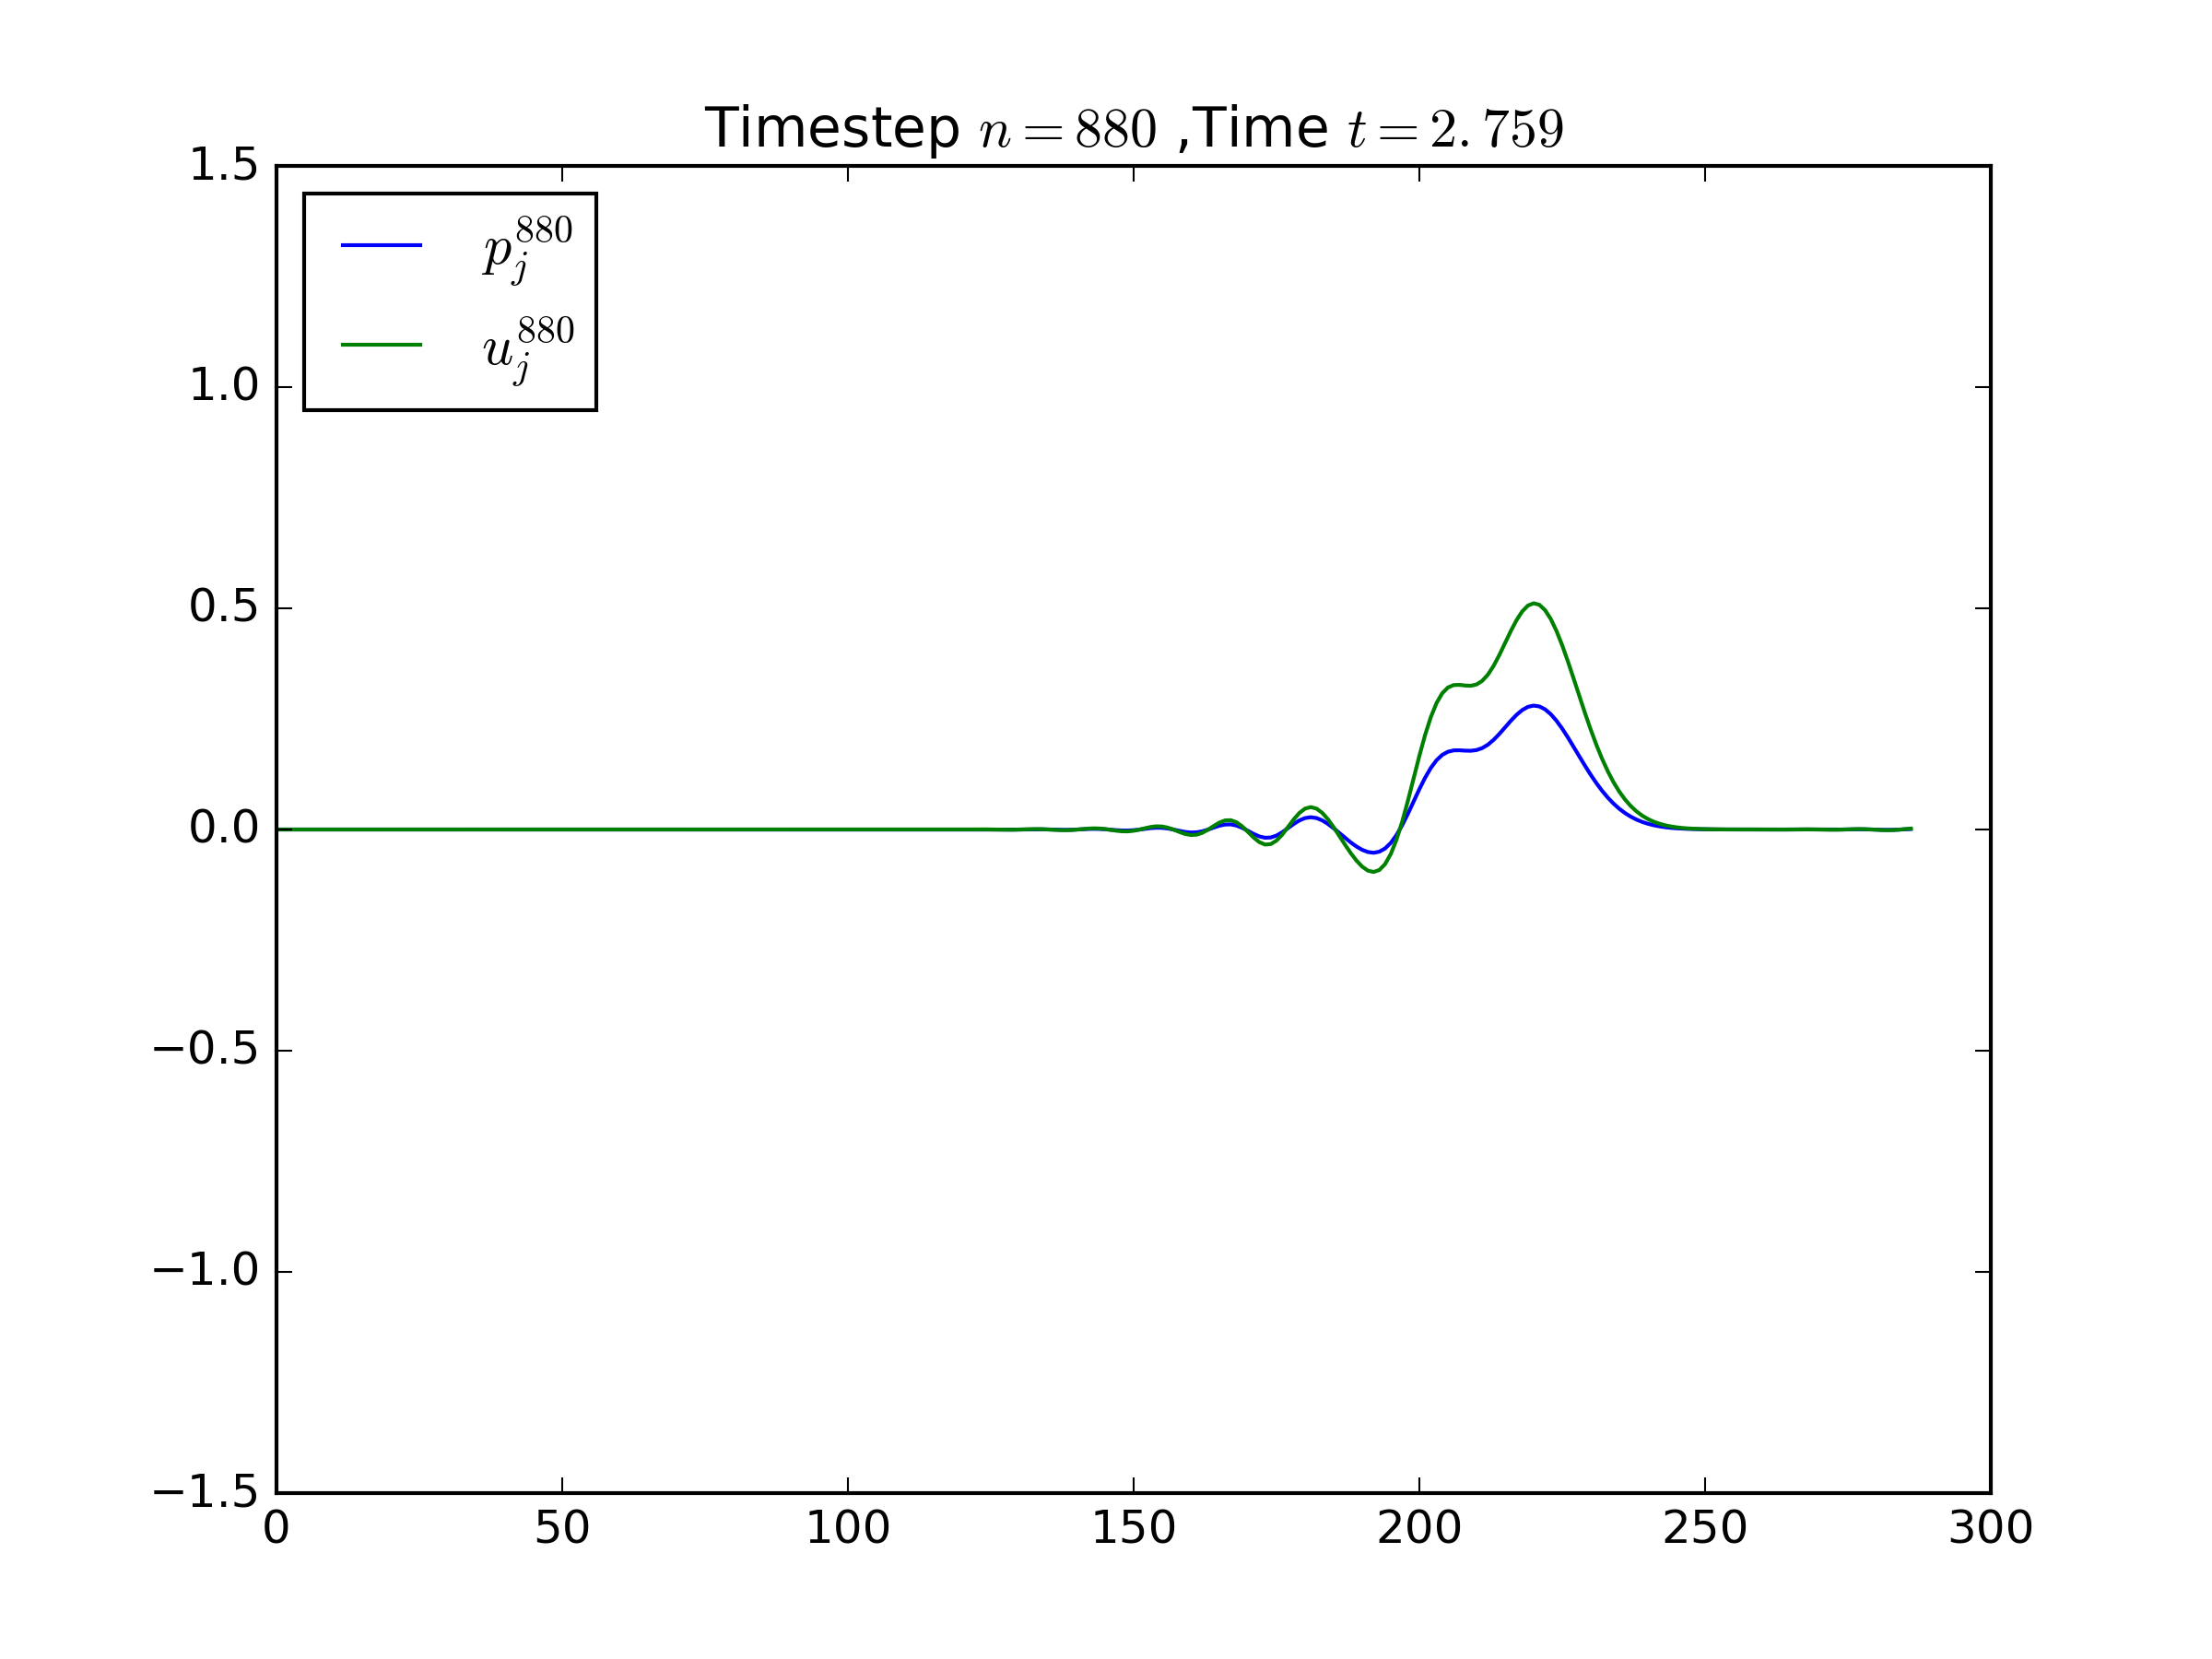
\includegraphics[width=0.31\textwidth]{figures/problem_1_b_088.png}
            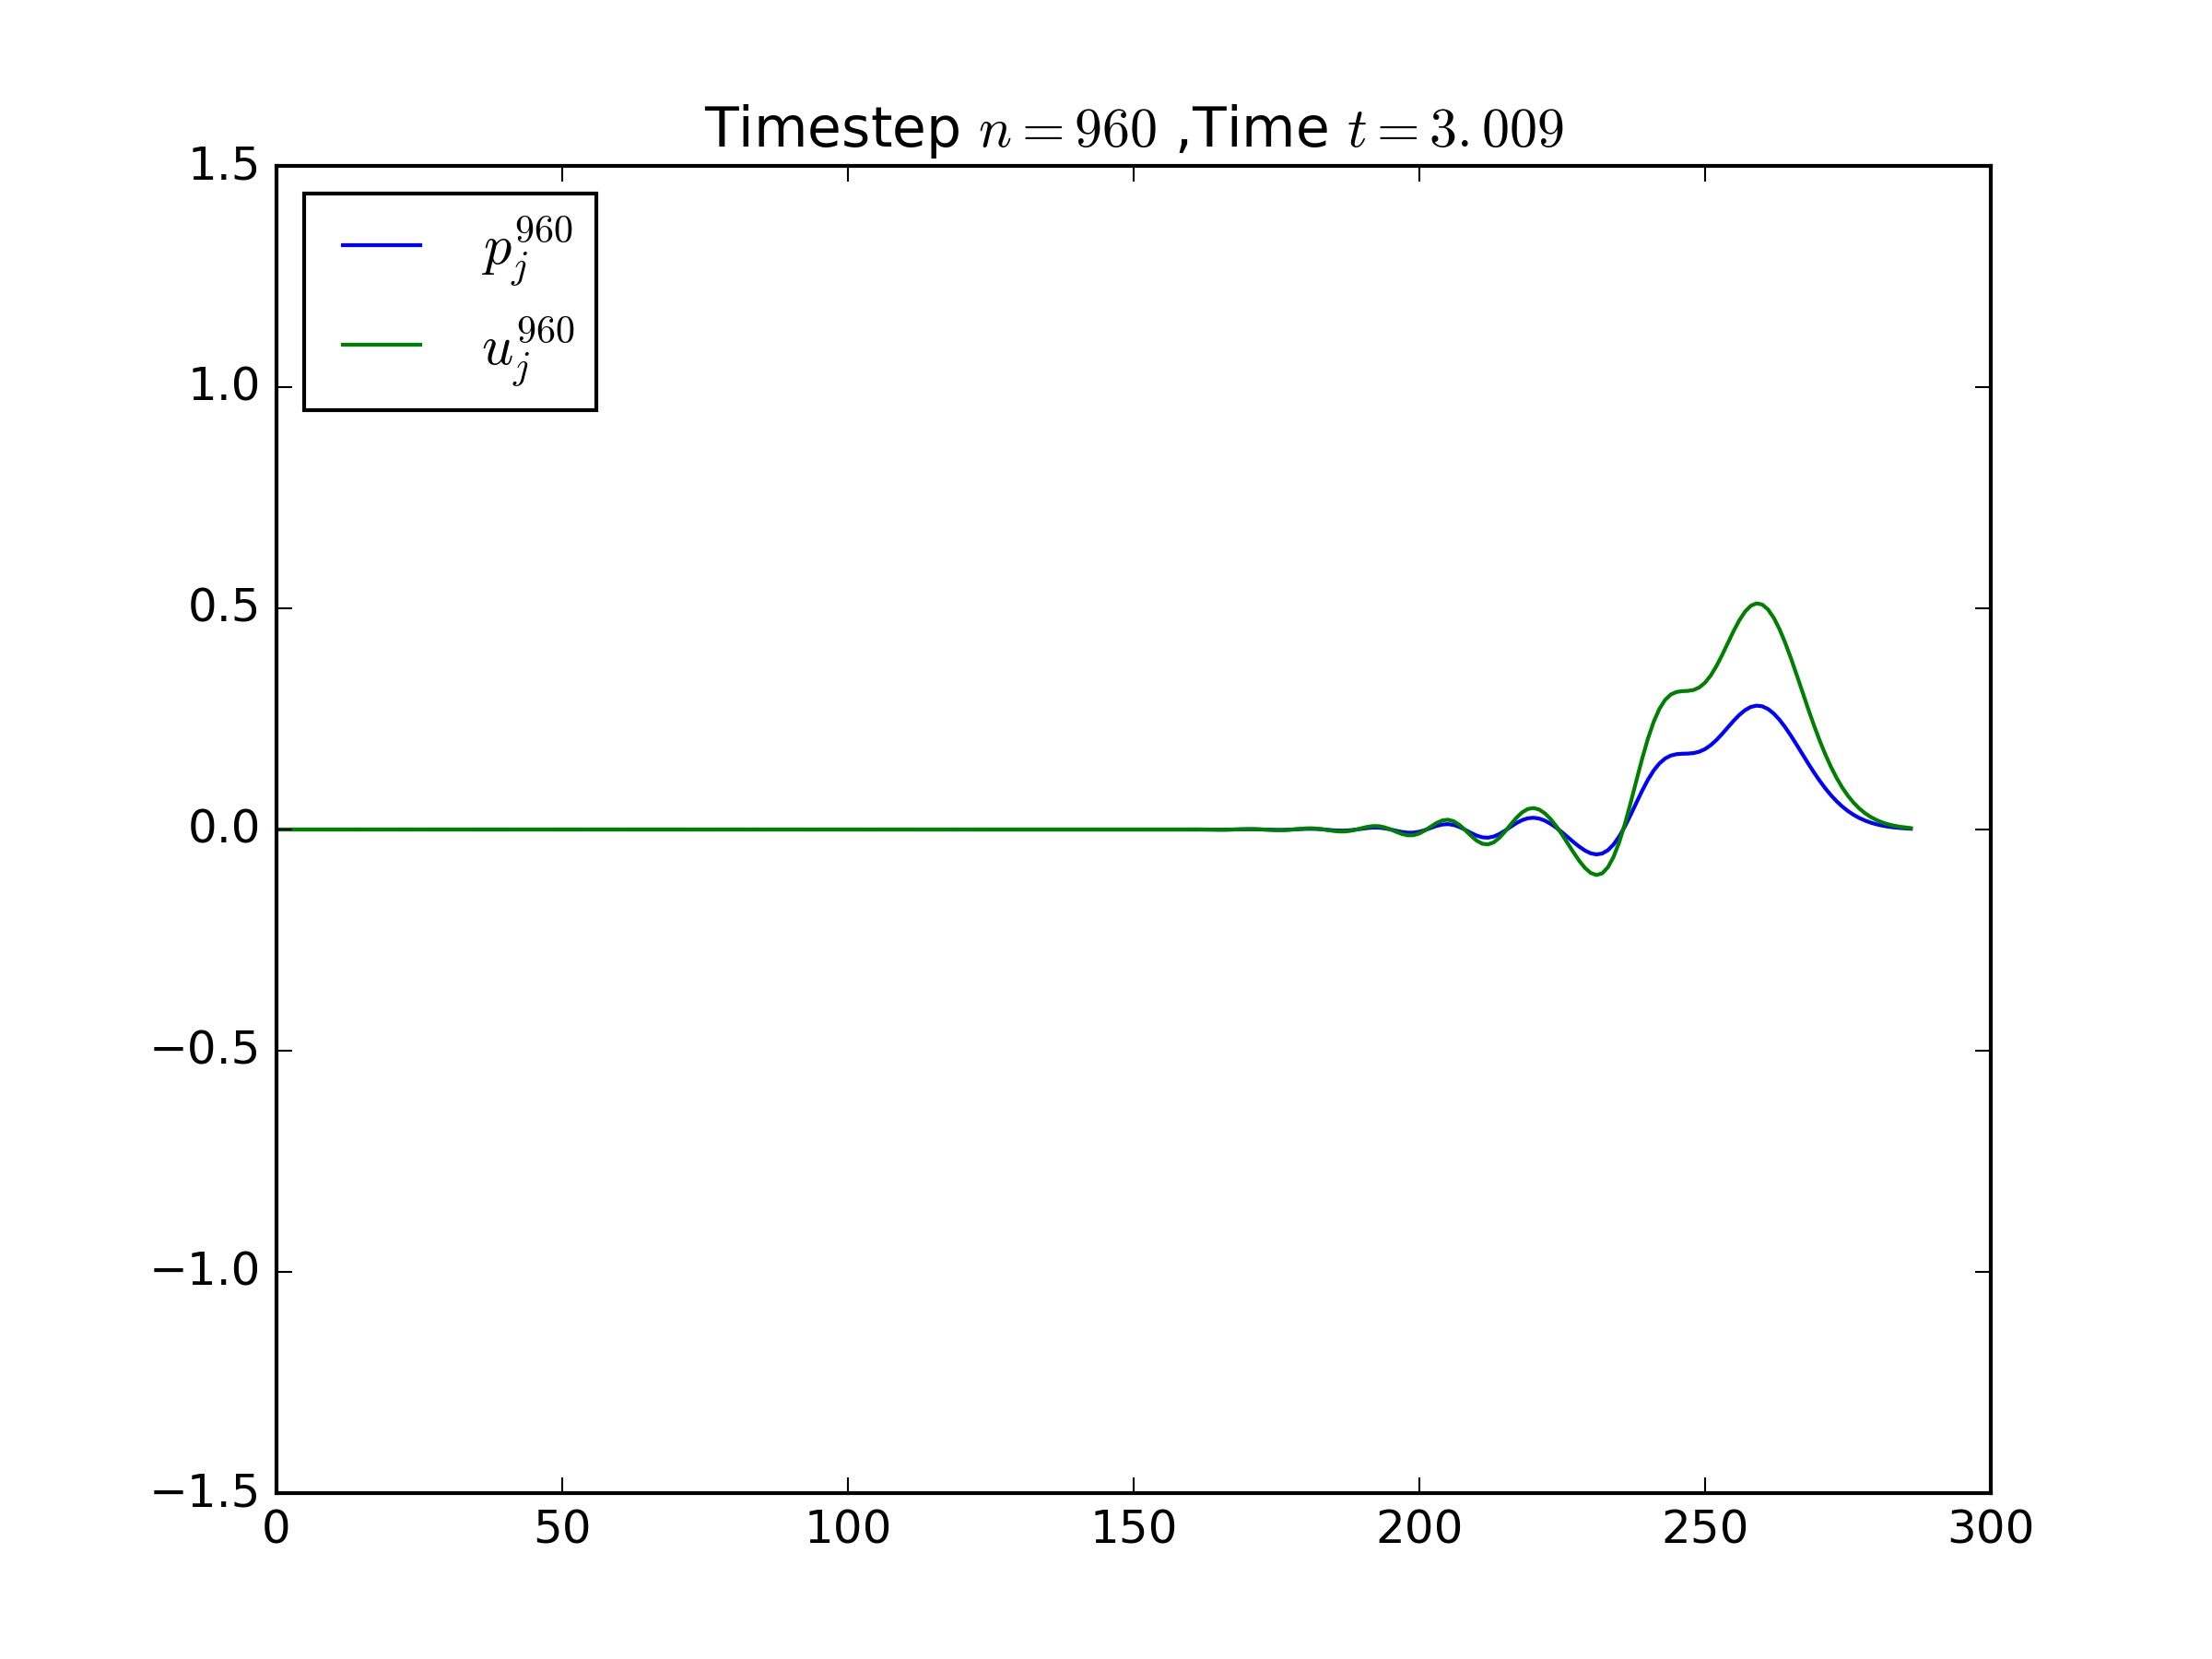
\includegraphics[width=0.31\textwidth]{figures/problem_1_b_096.png}
            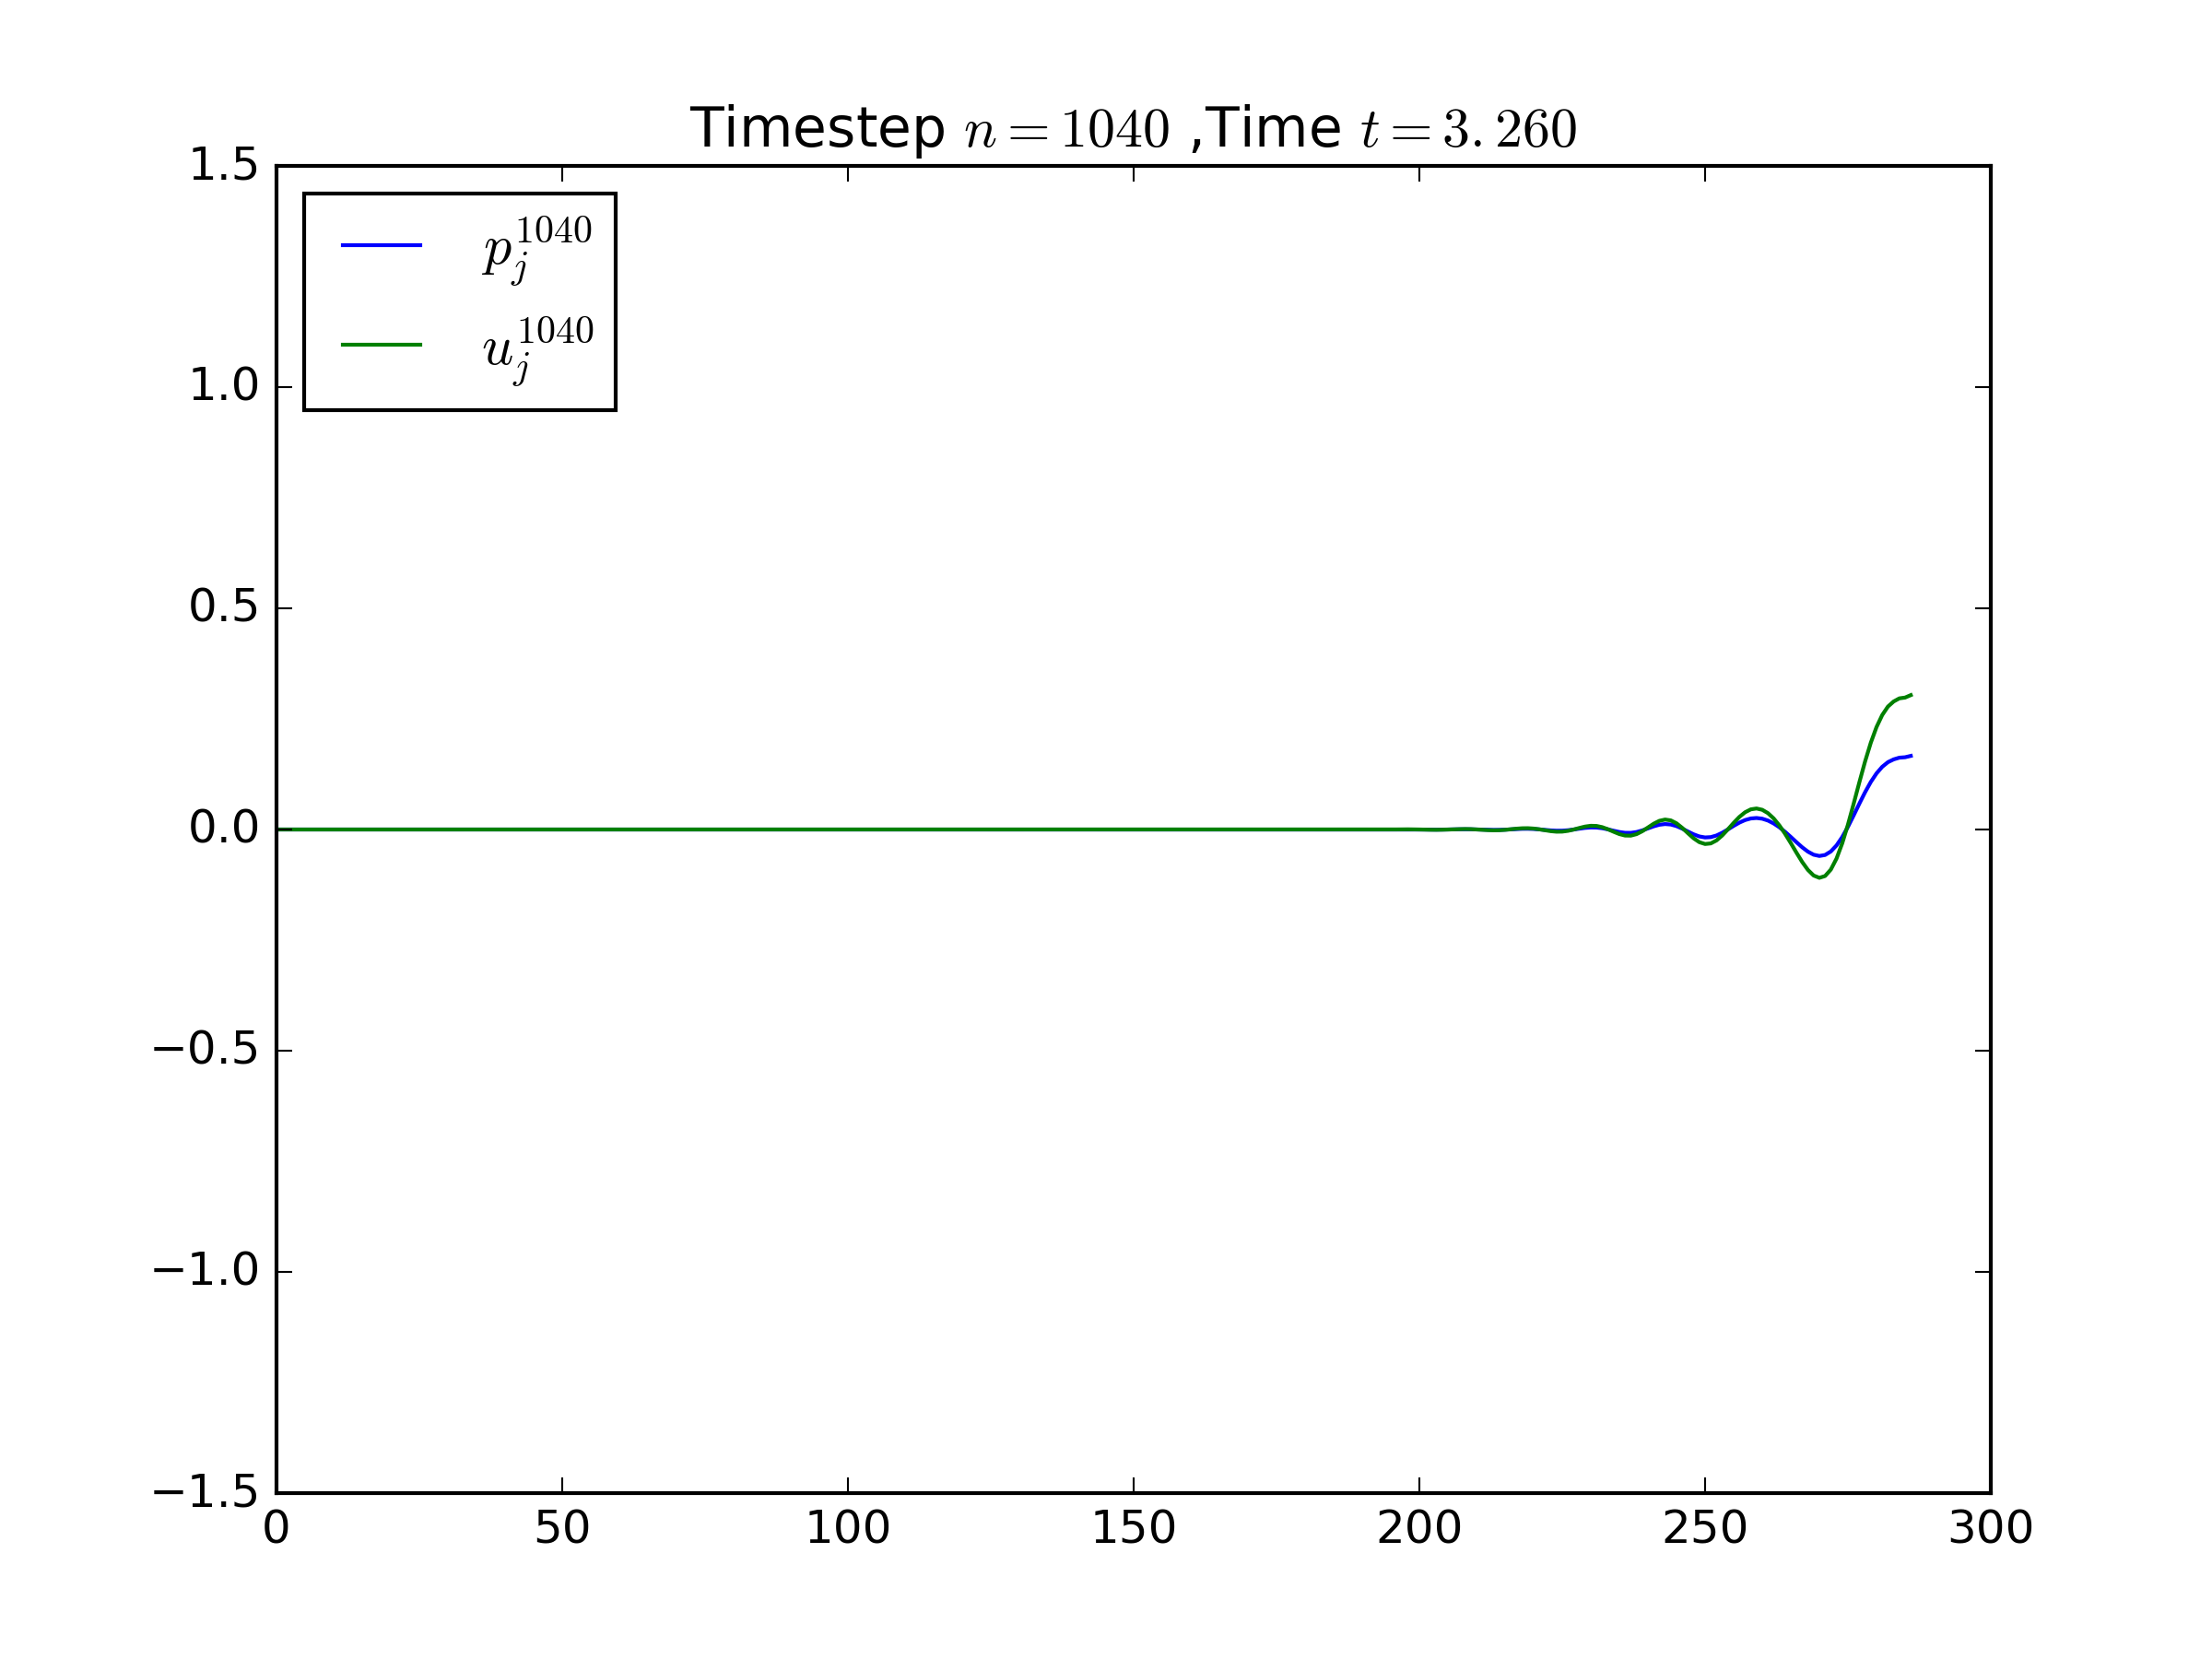
\includegraphics[width=0.31\textwidth]{figures/problem_1_b_104.png}
            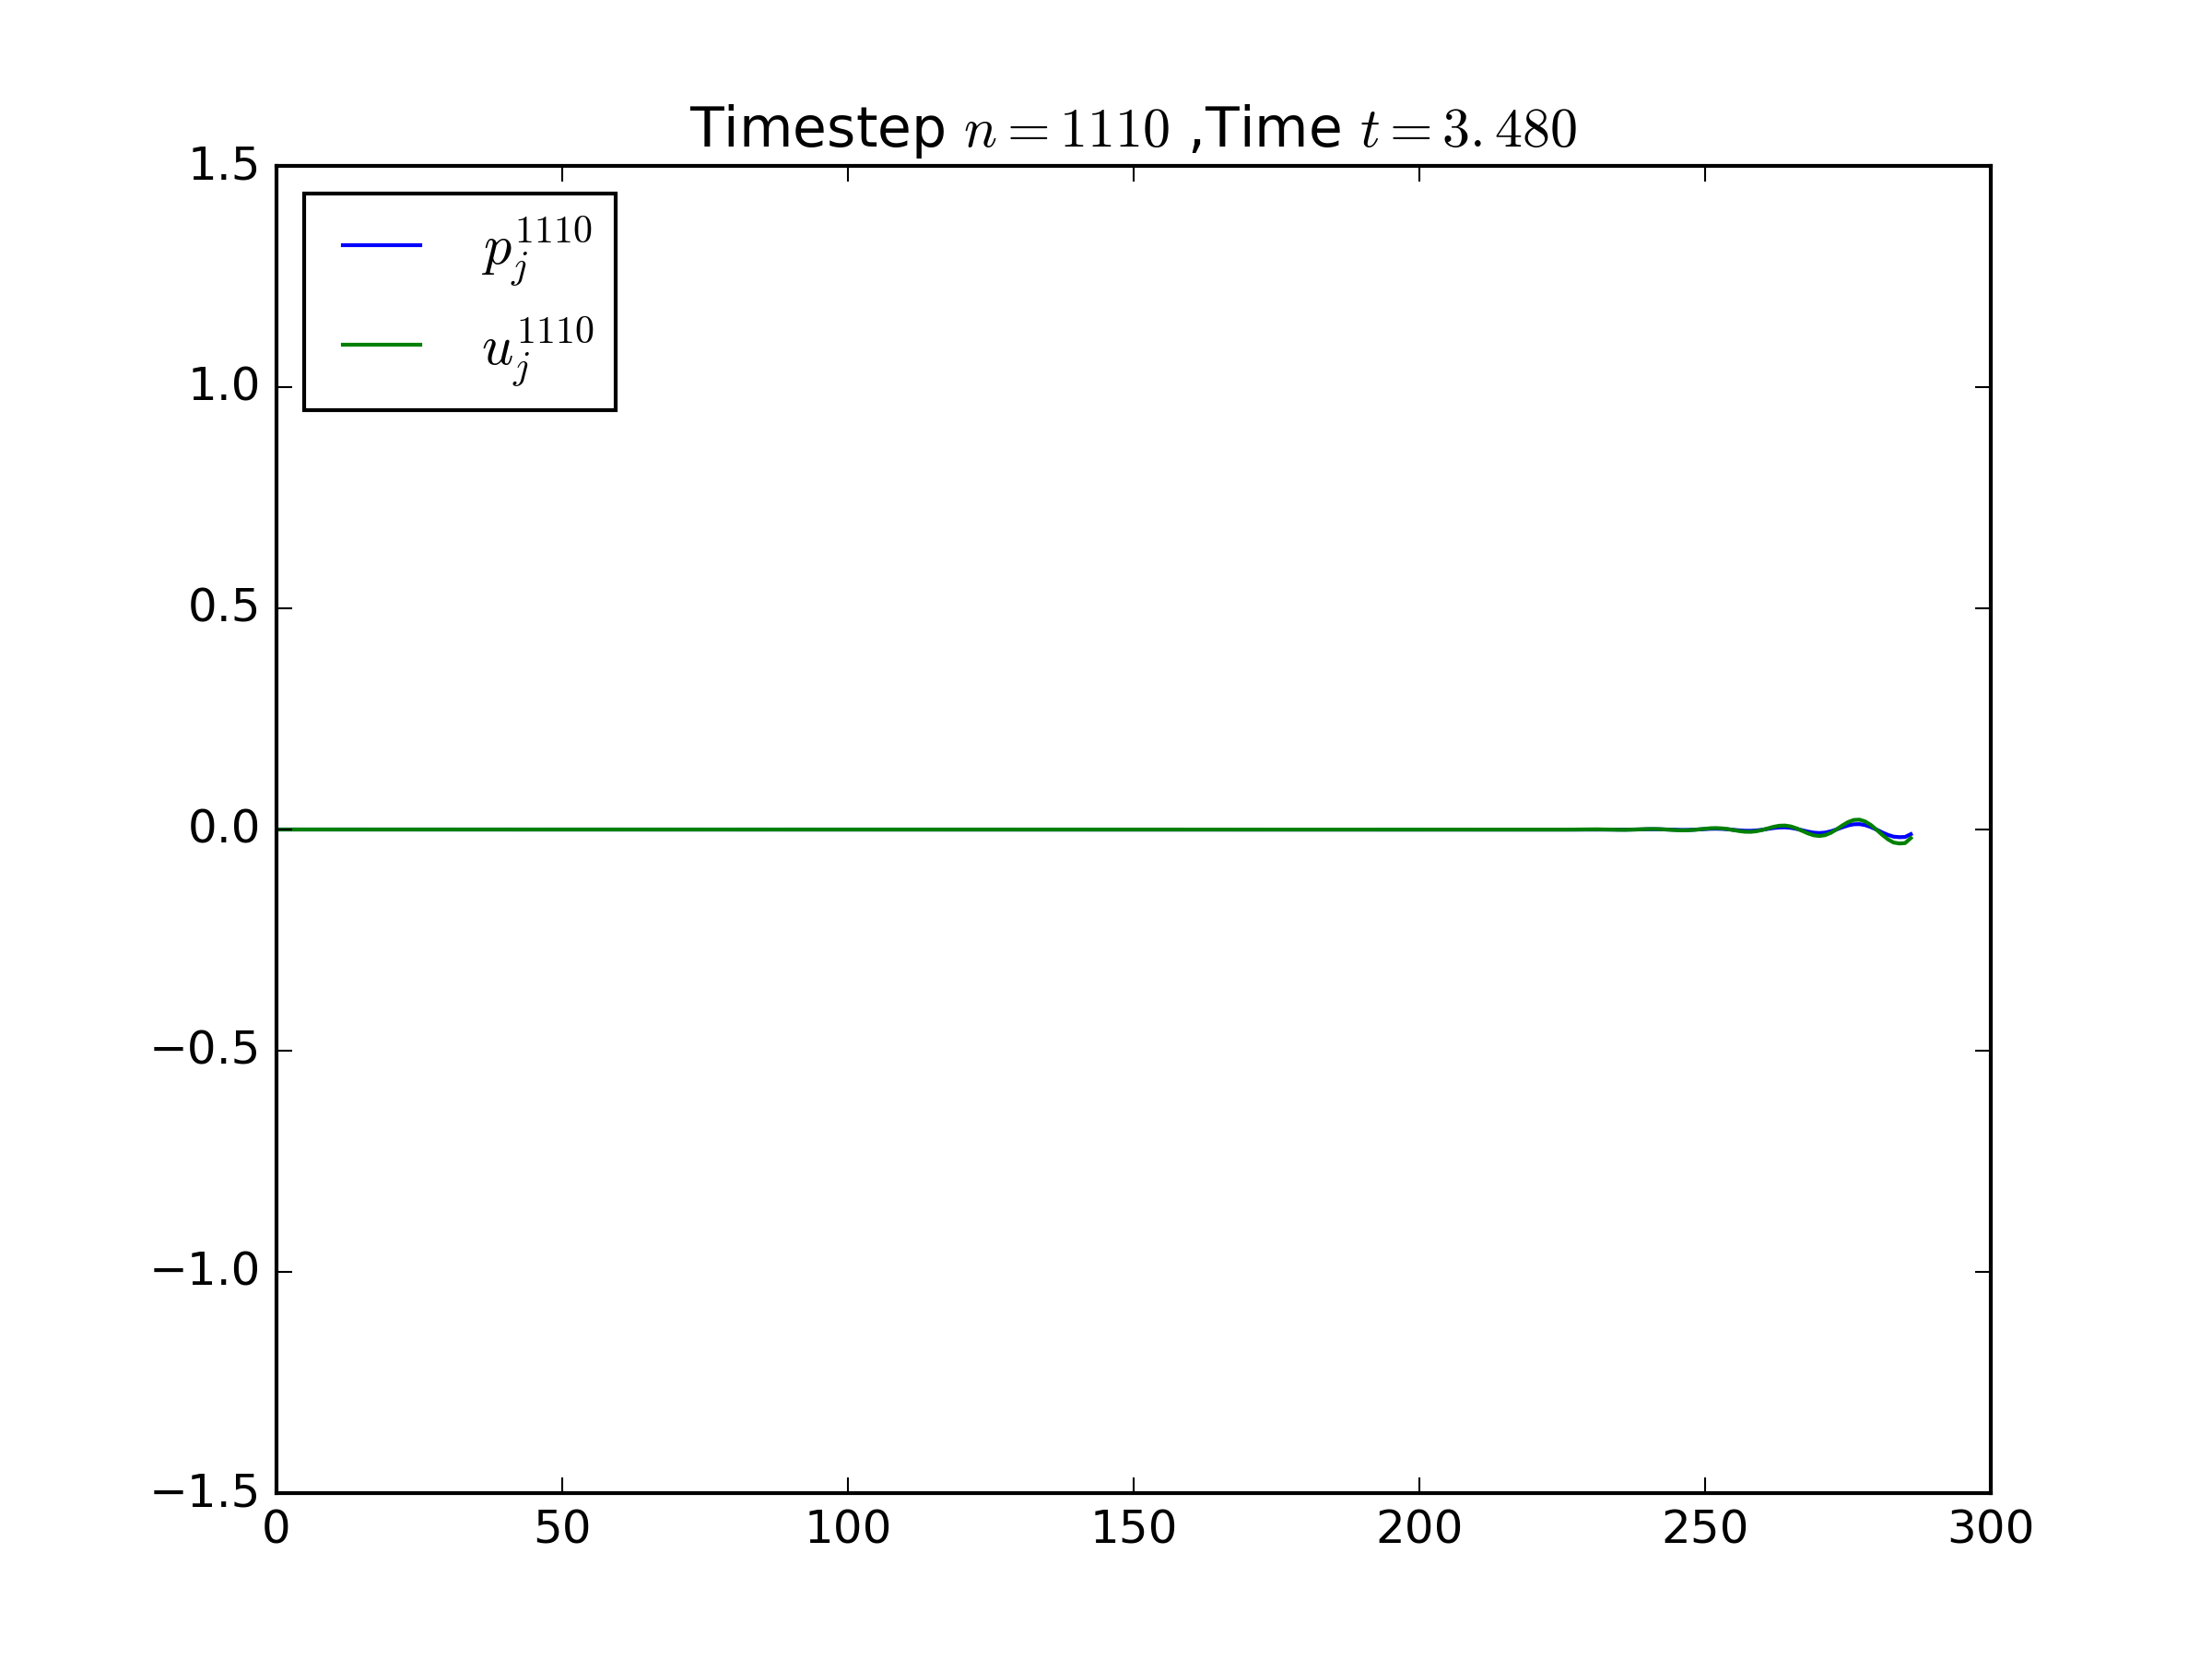
\includegraphics[width=0.31\textwidth]{figures/problem_1_b_111.png}
        \end{figure}
        \FloatBarrier
        \pagebreak

        The initial behavior of this system is much more difficult to see for low frequency initial data which spans the entire region.  However we do see a diffused initial condition (with $u$ turned upside-down) move to the right, just like the above simulations, once the large wave exits the right side and the small wave is finished bouncing off the left side.  Here are the results:
        \begin{figure}[ht!]
            \centering
            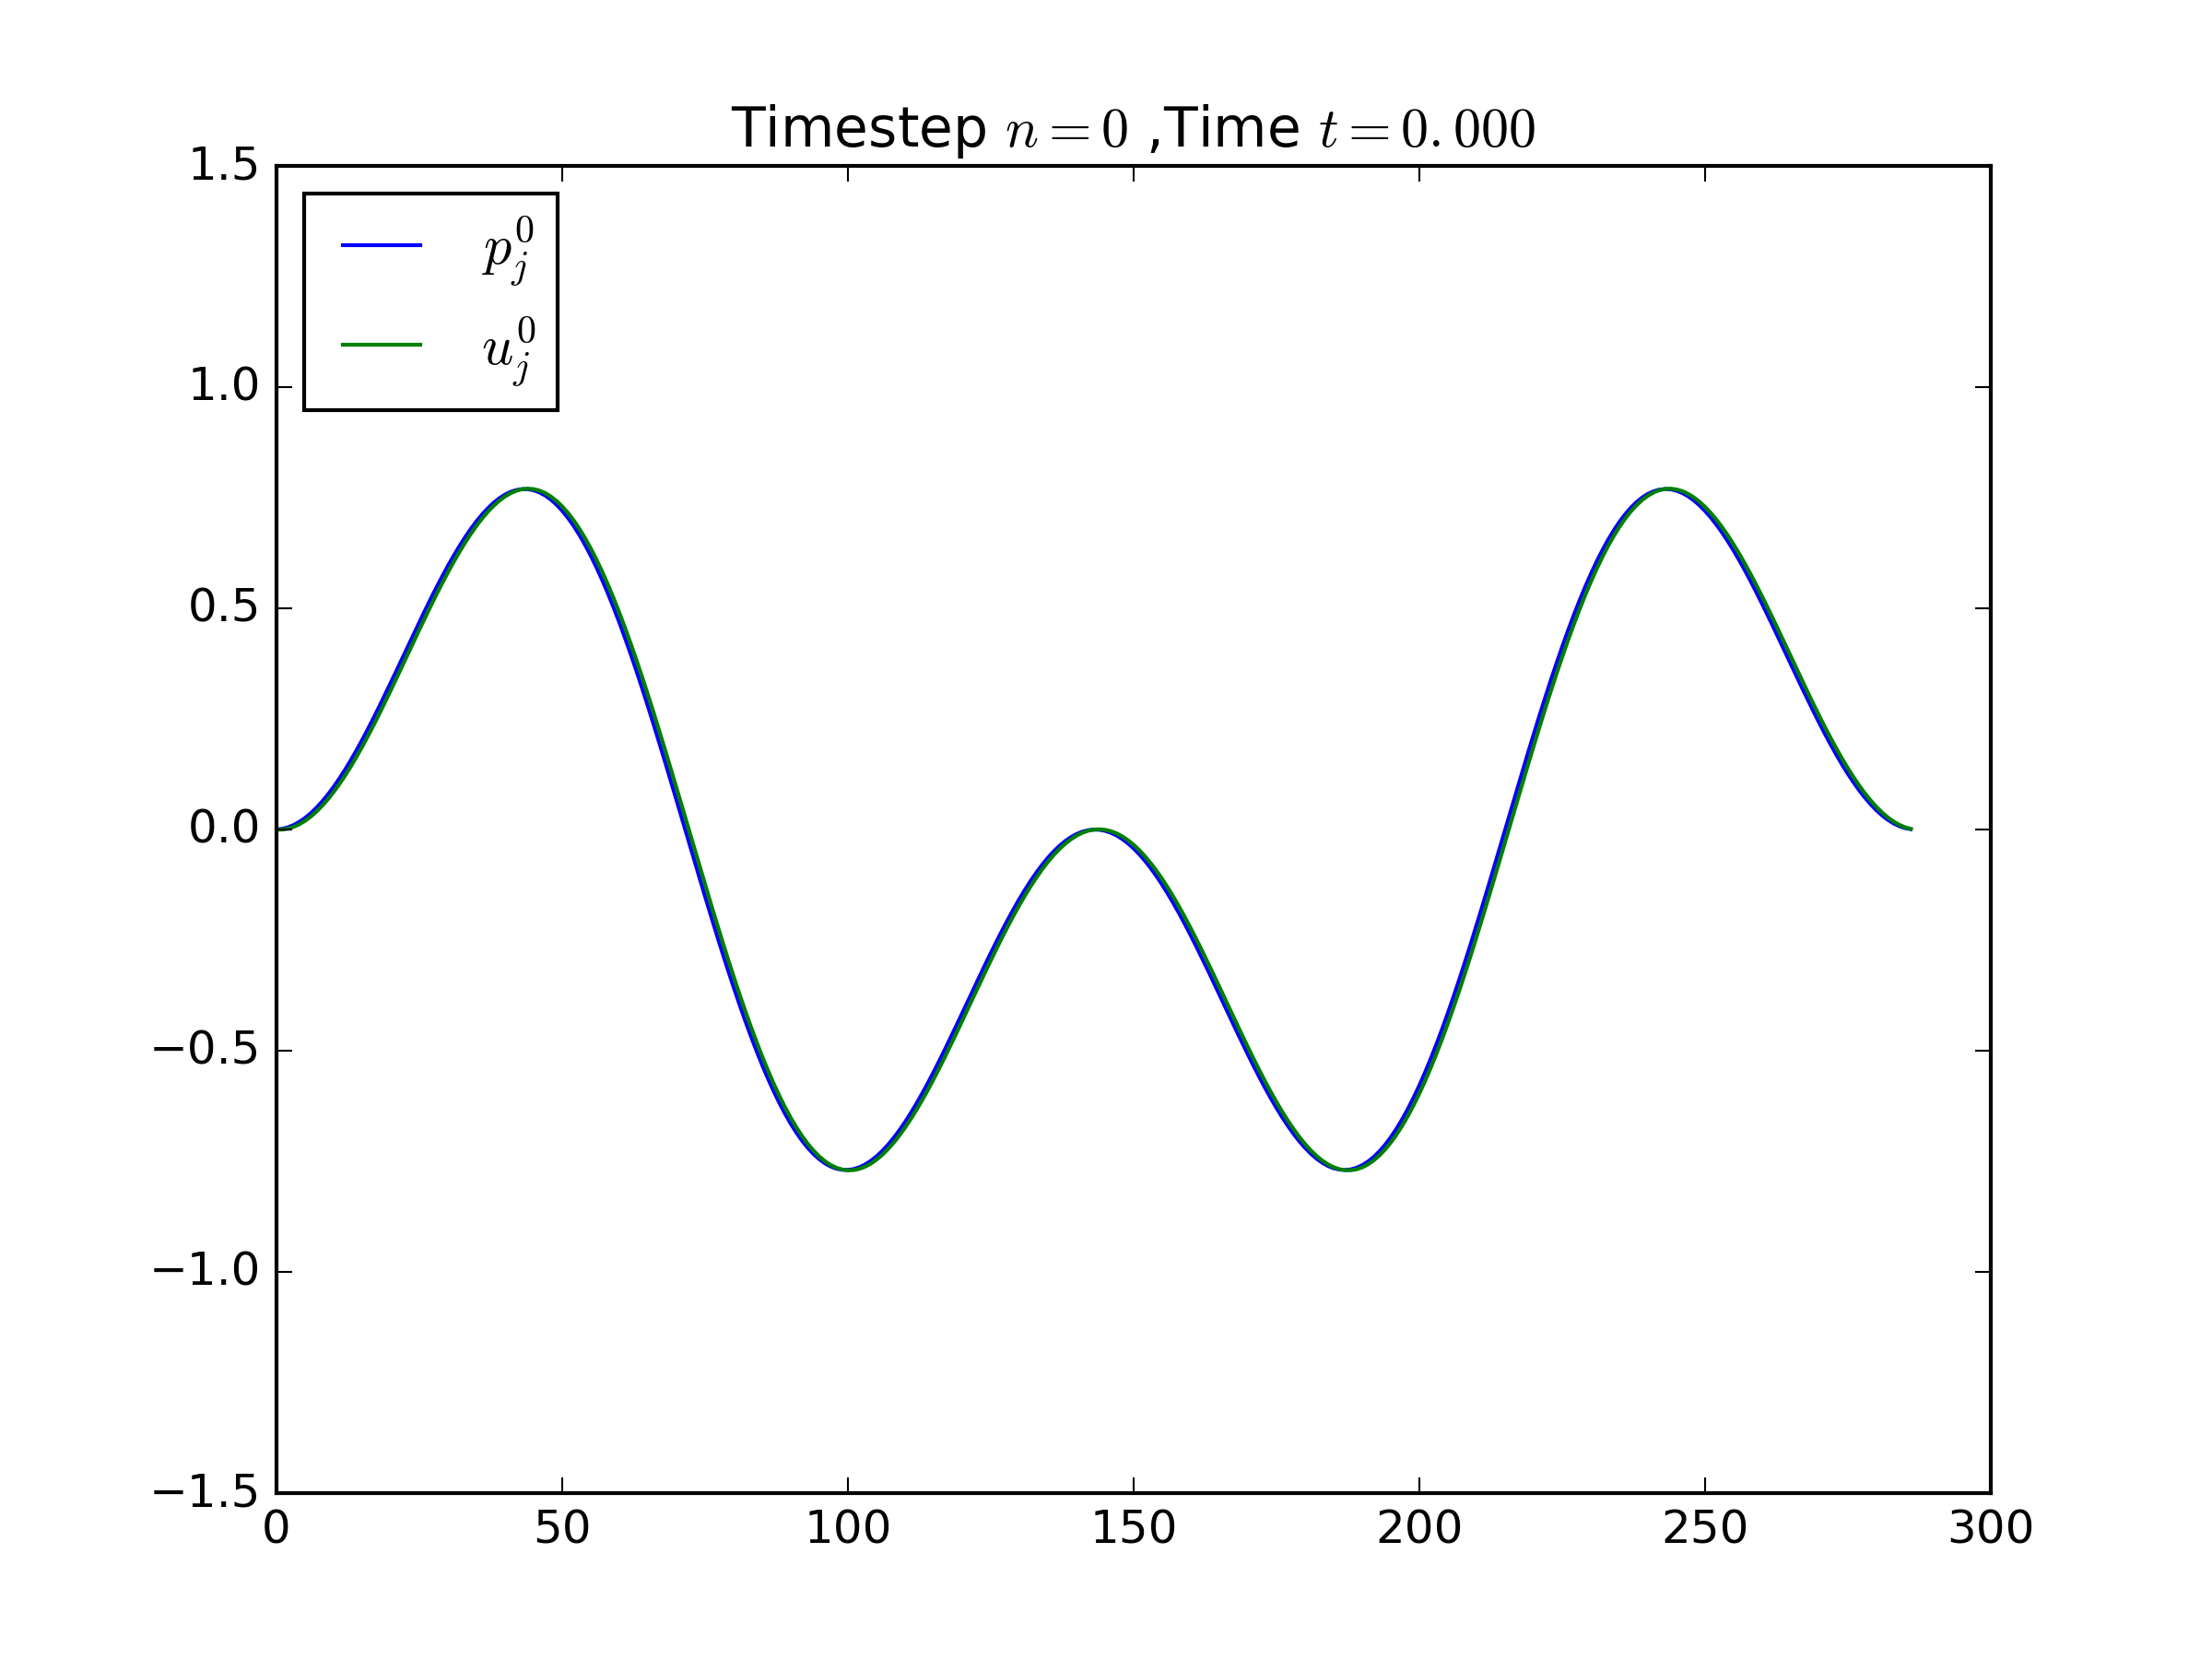
\includegraphics[width=0.31\textwidth]{figures/problem_1_c_000.png}
            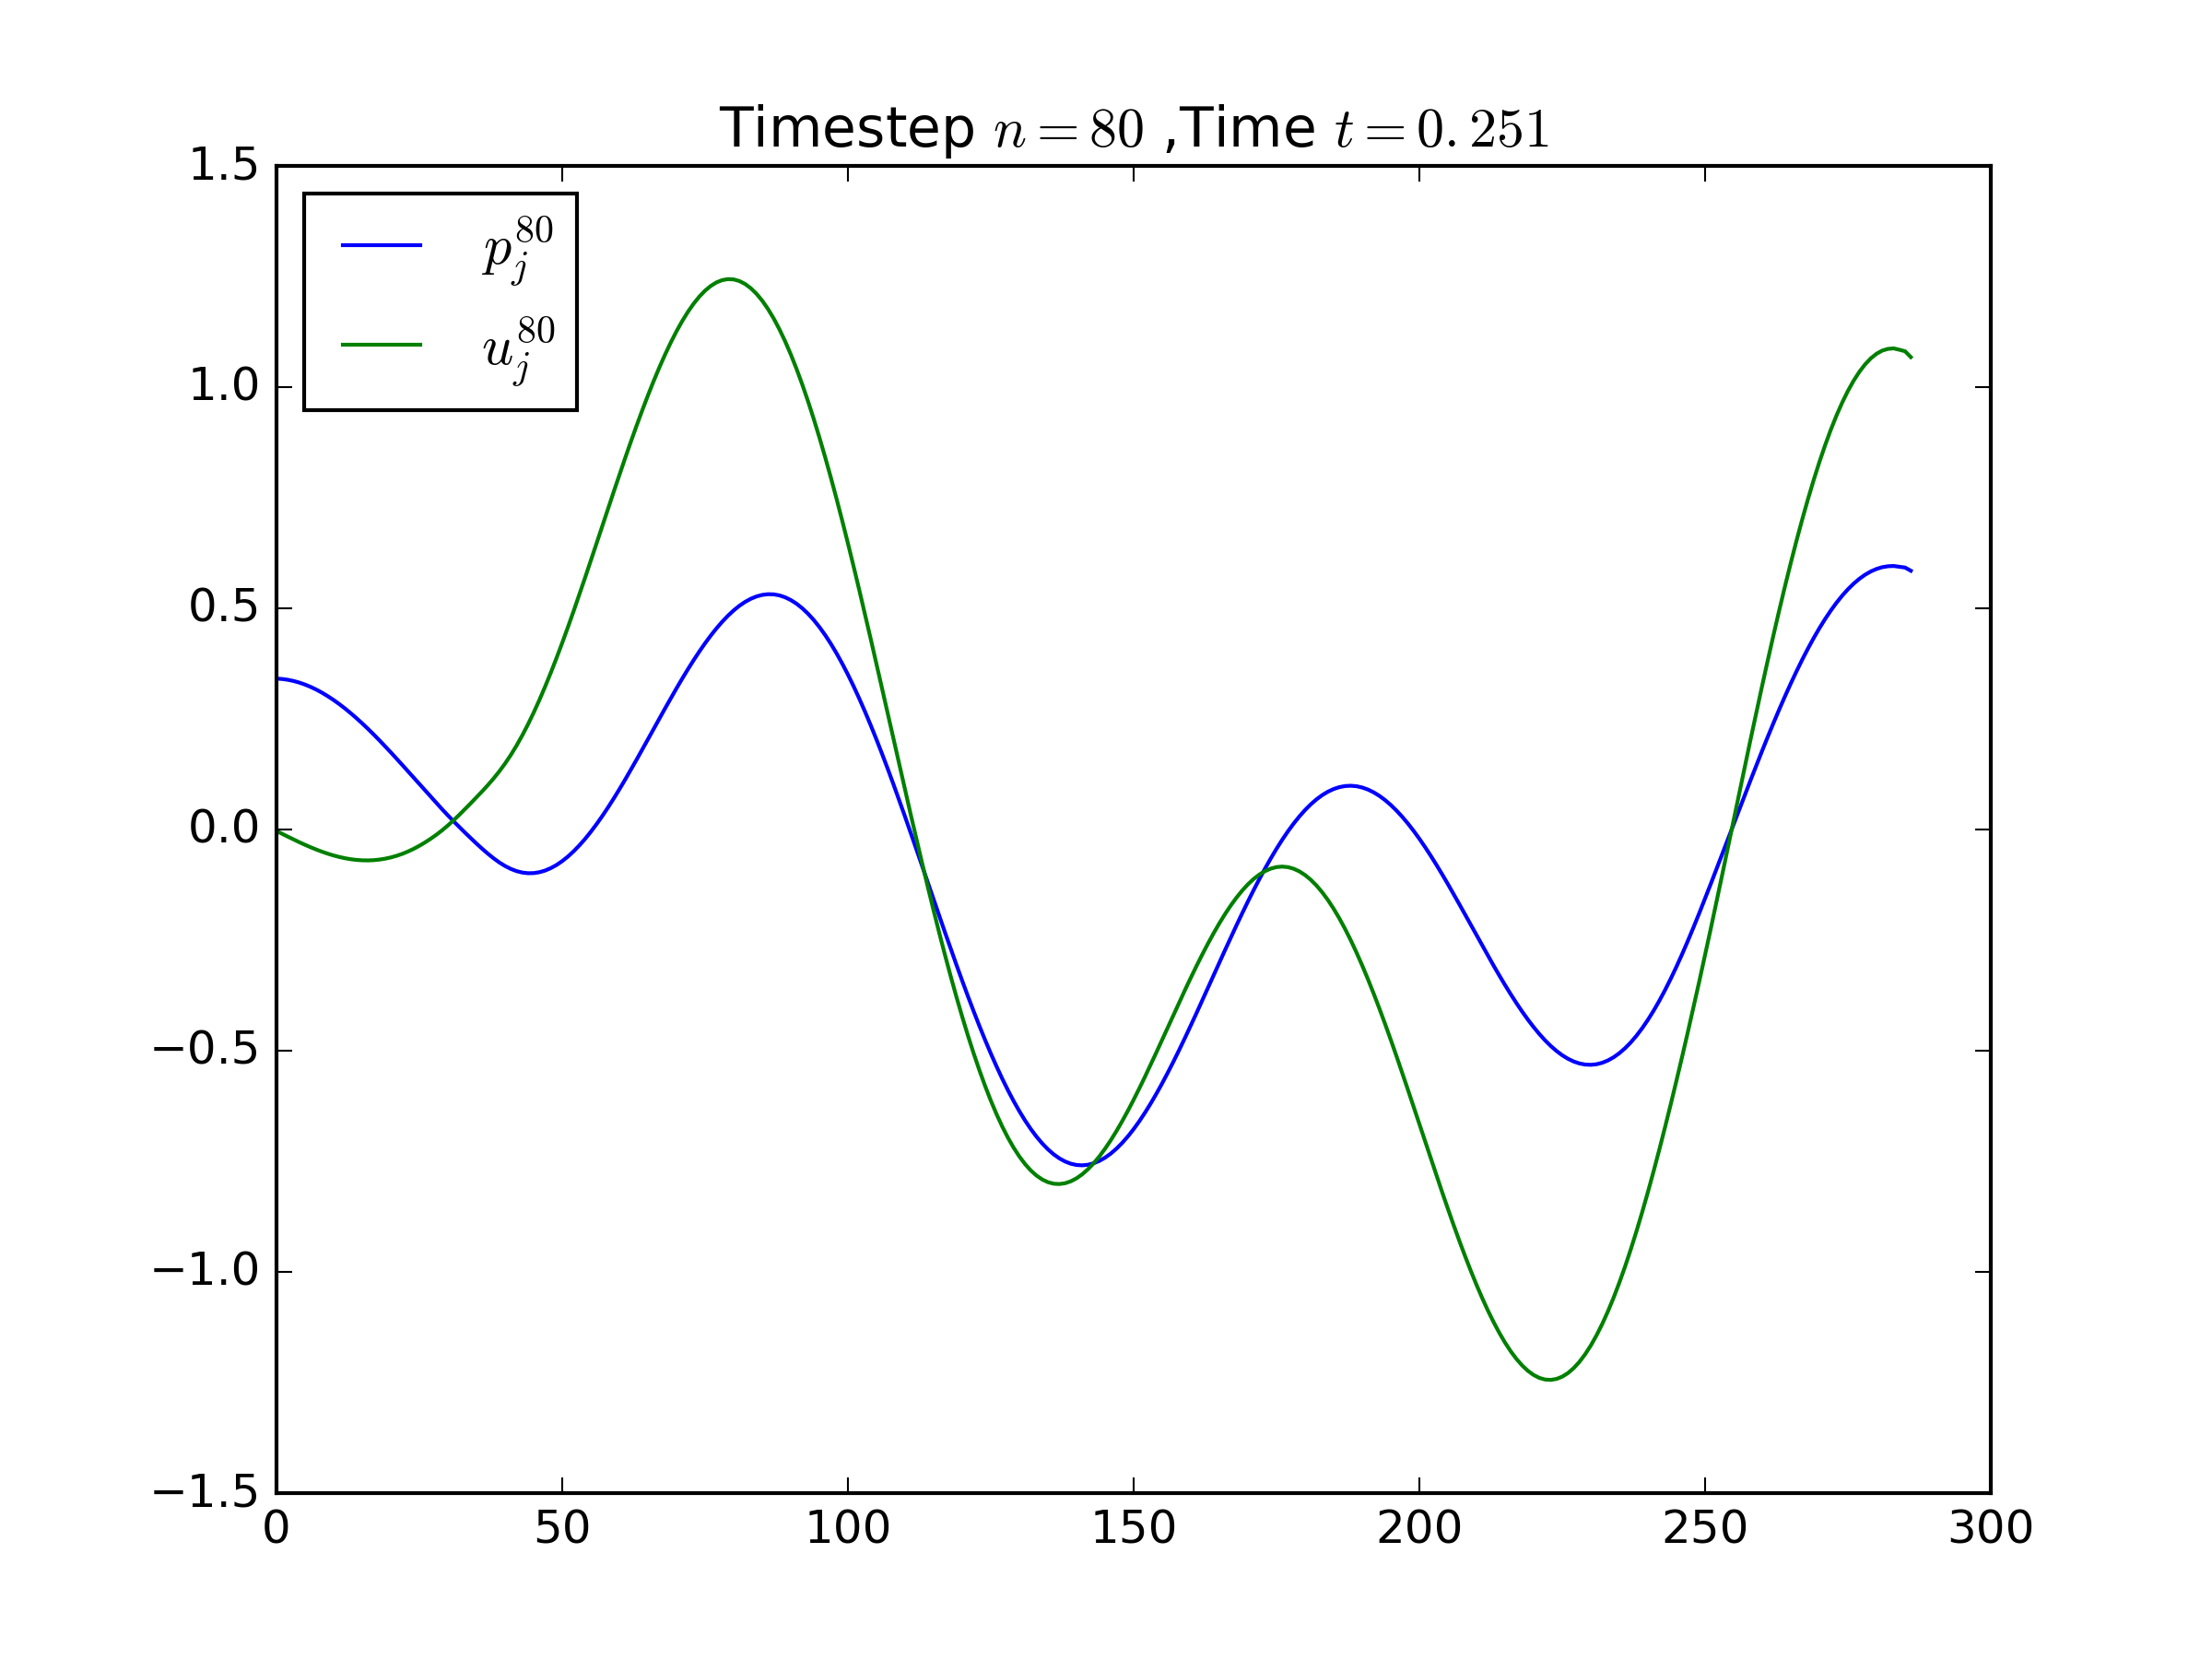
\includegraphics[width=0.31\textwidth]{figures/problem_1_c_008.png}
            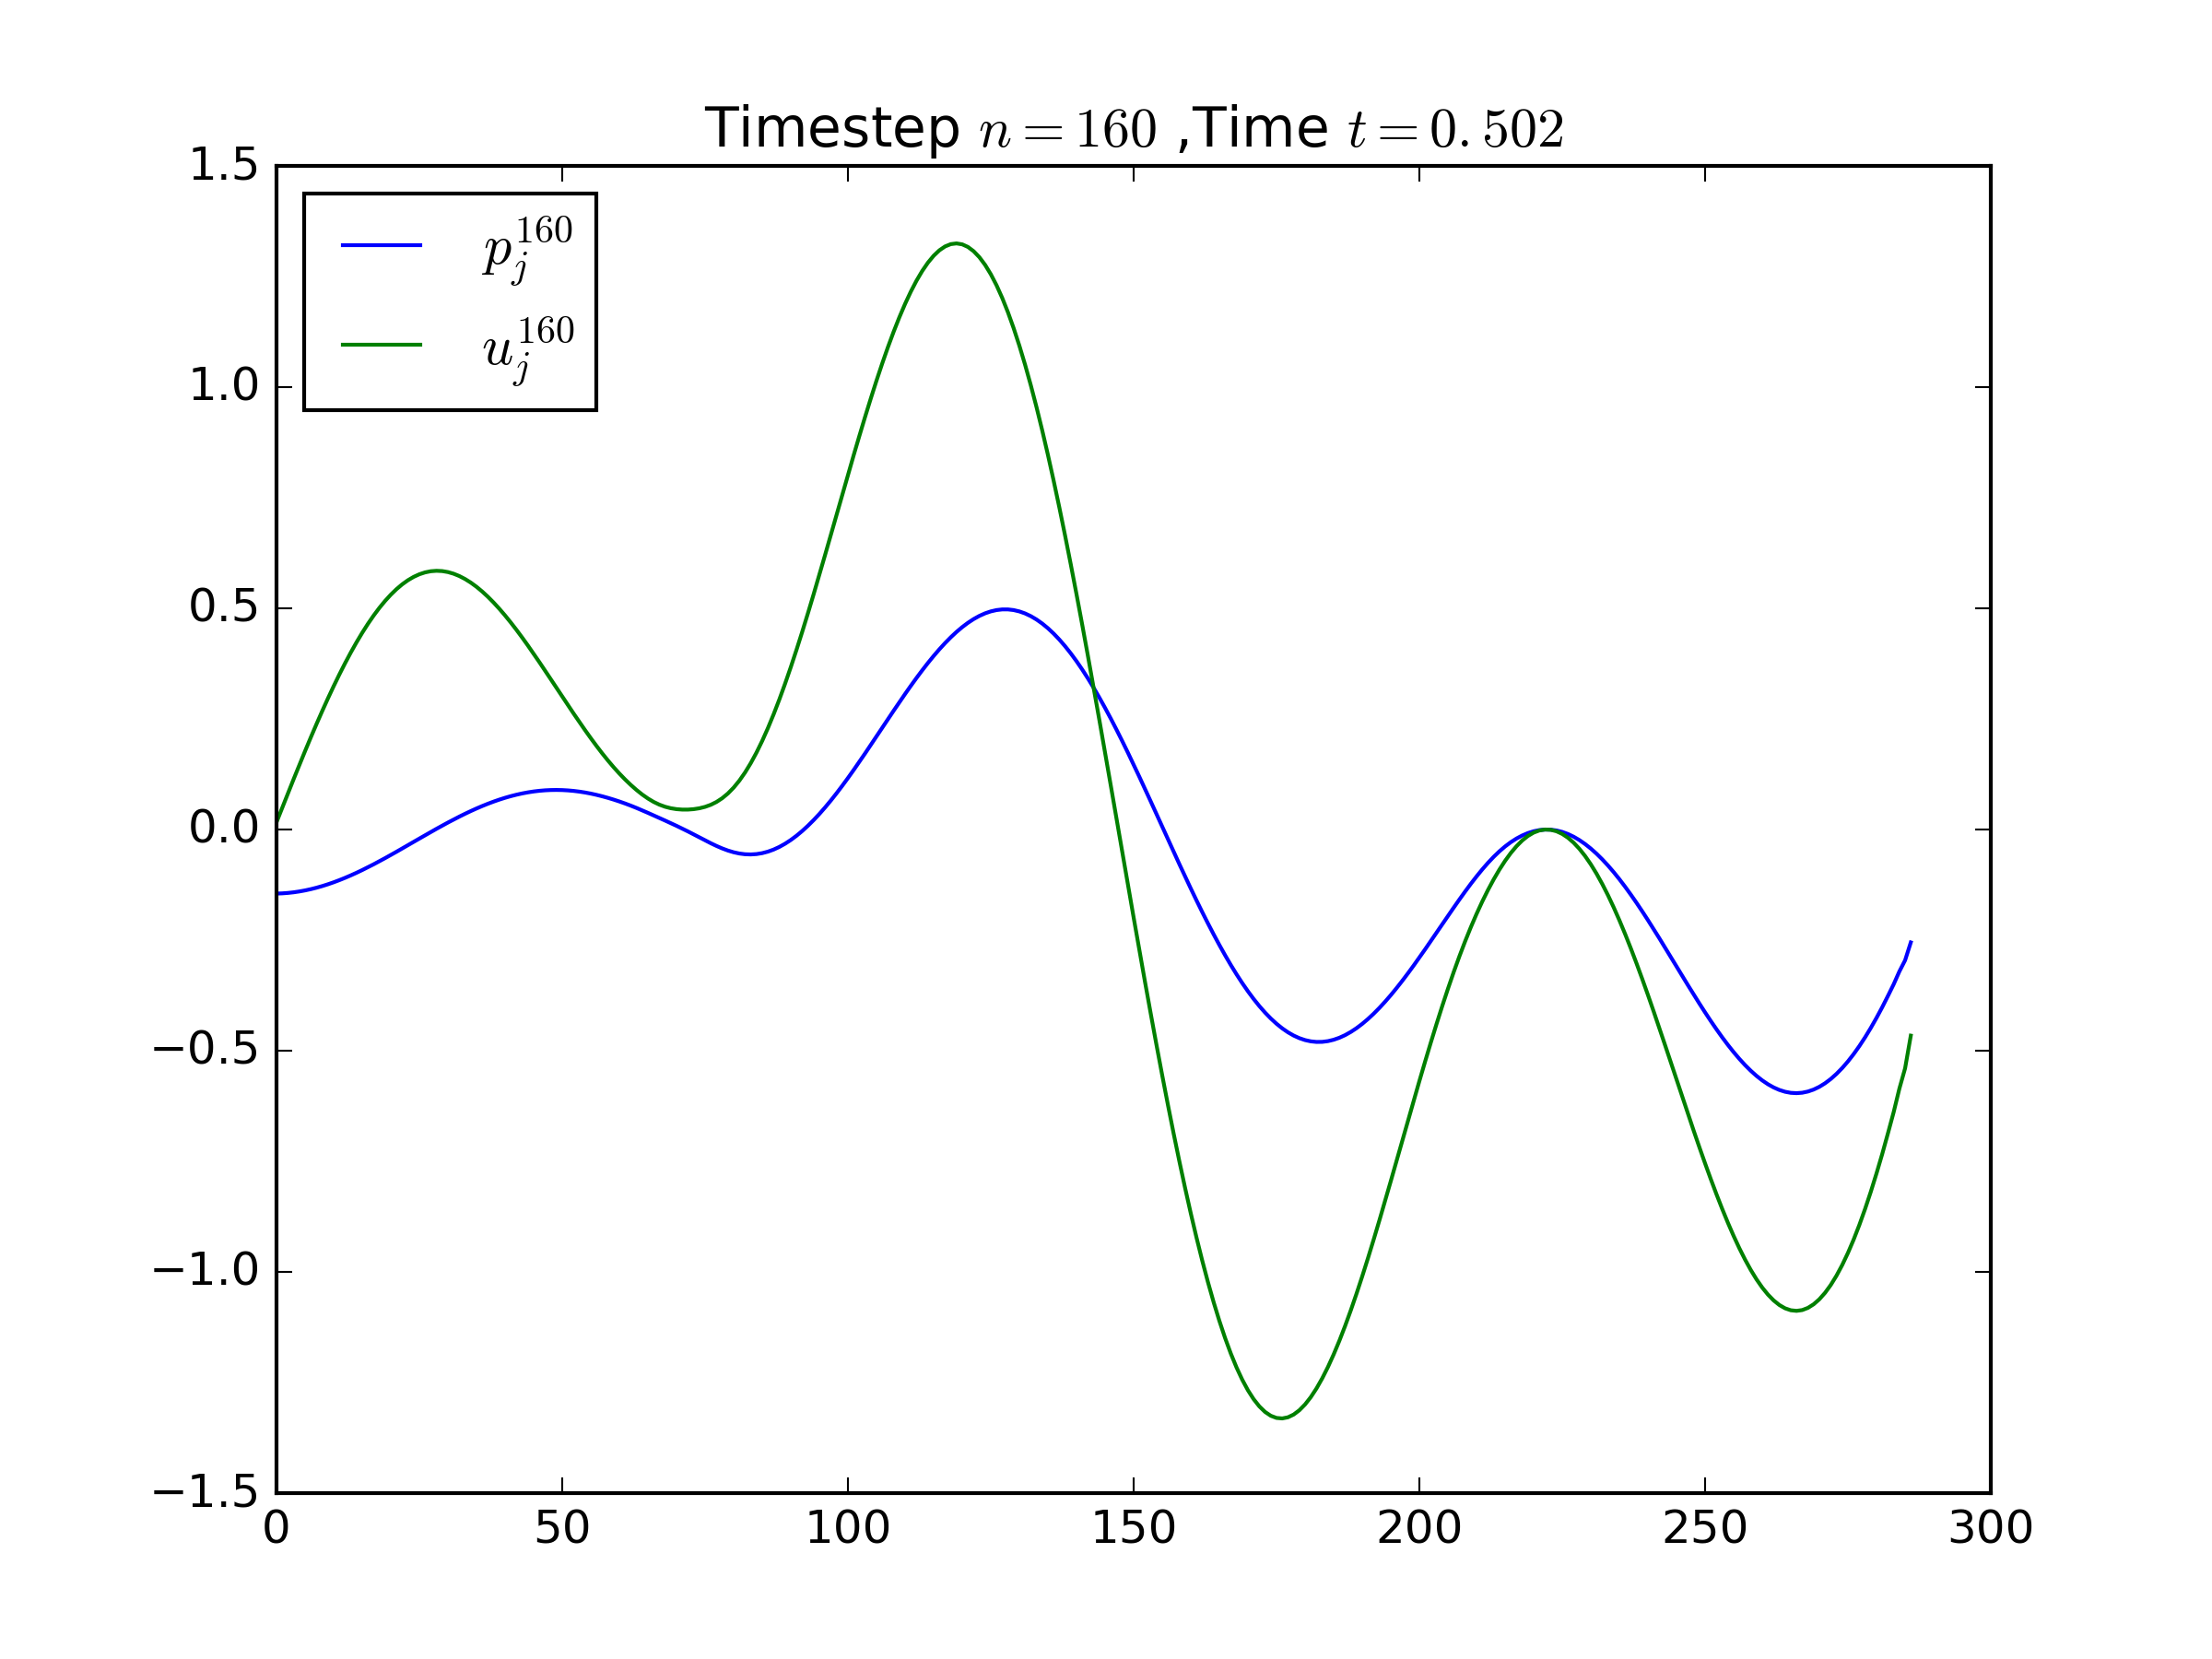
\includegraphics[width=0.31\textwidth]{figures/problem_1_c_016.png}
            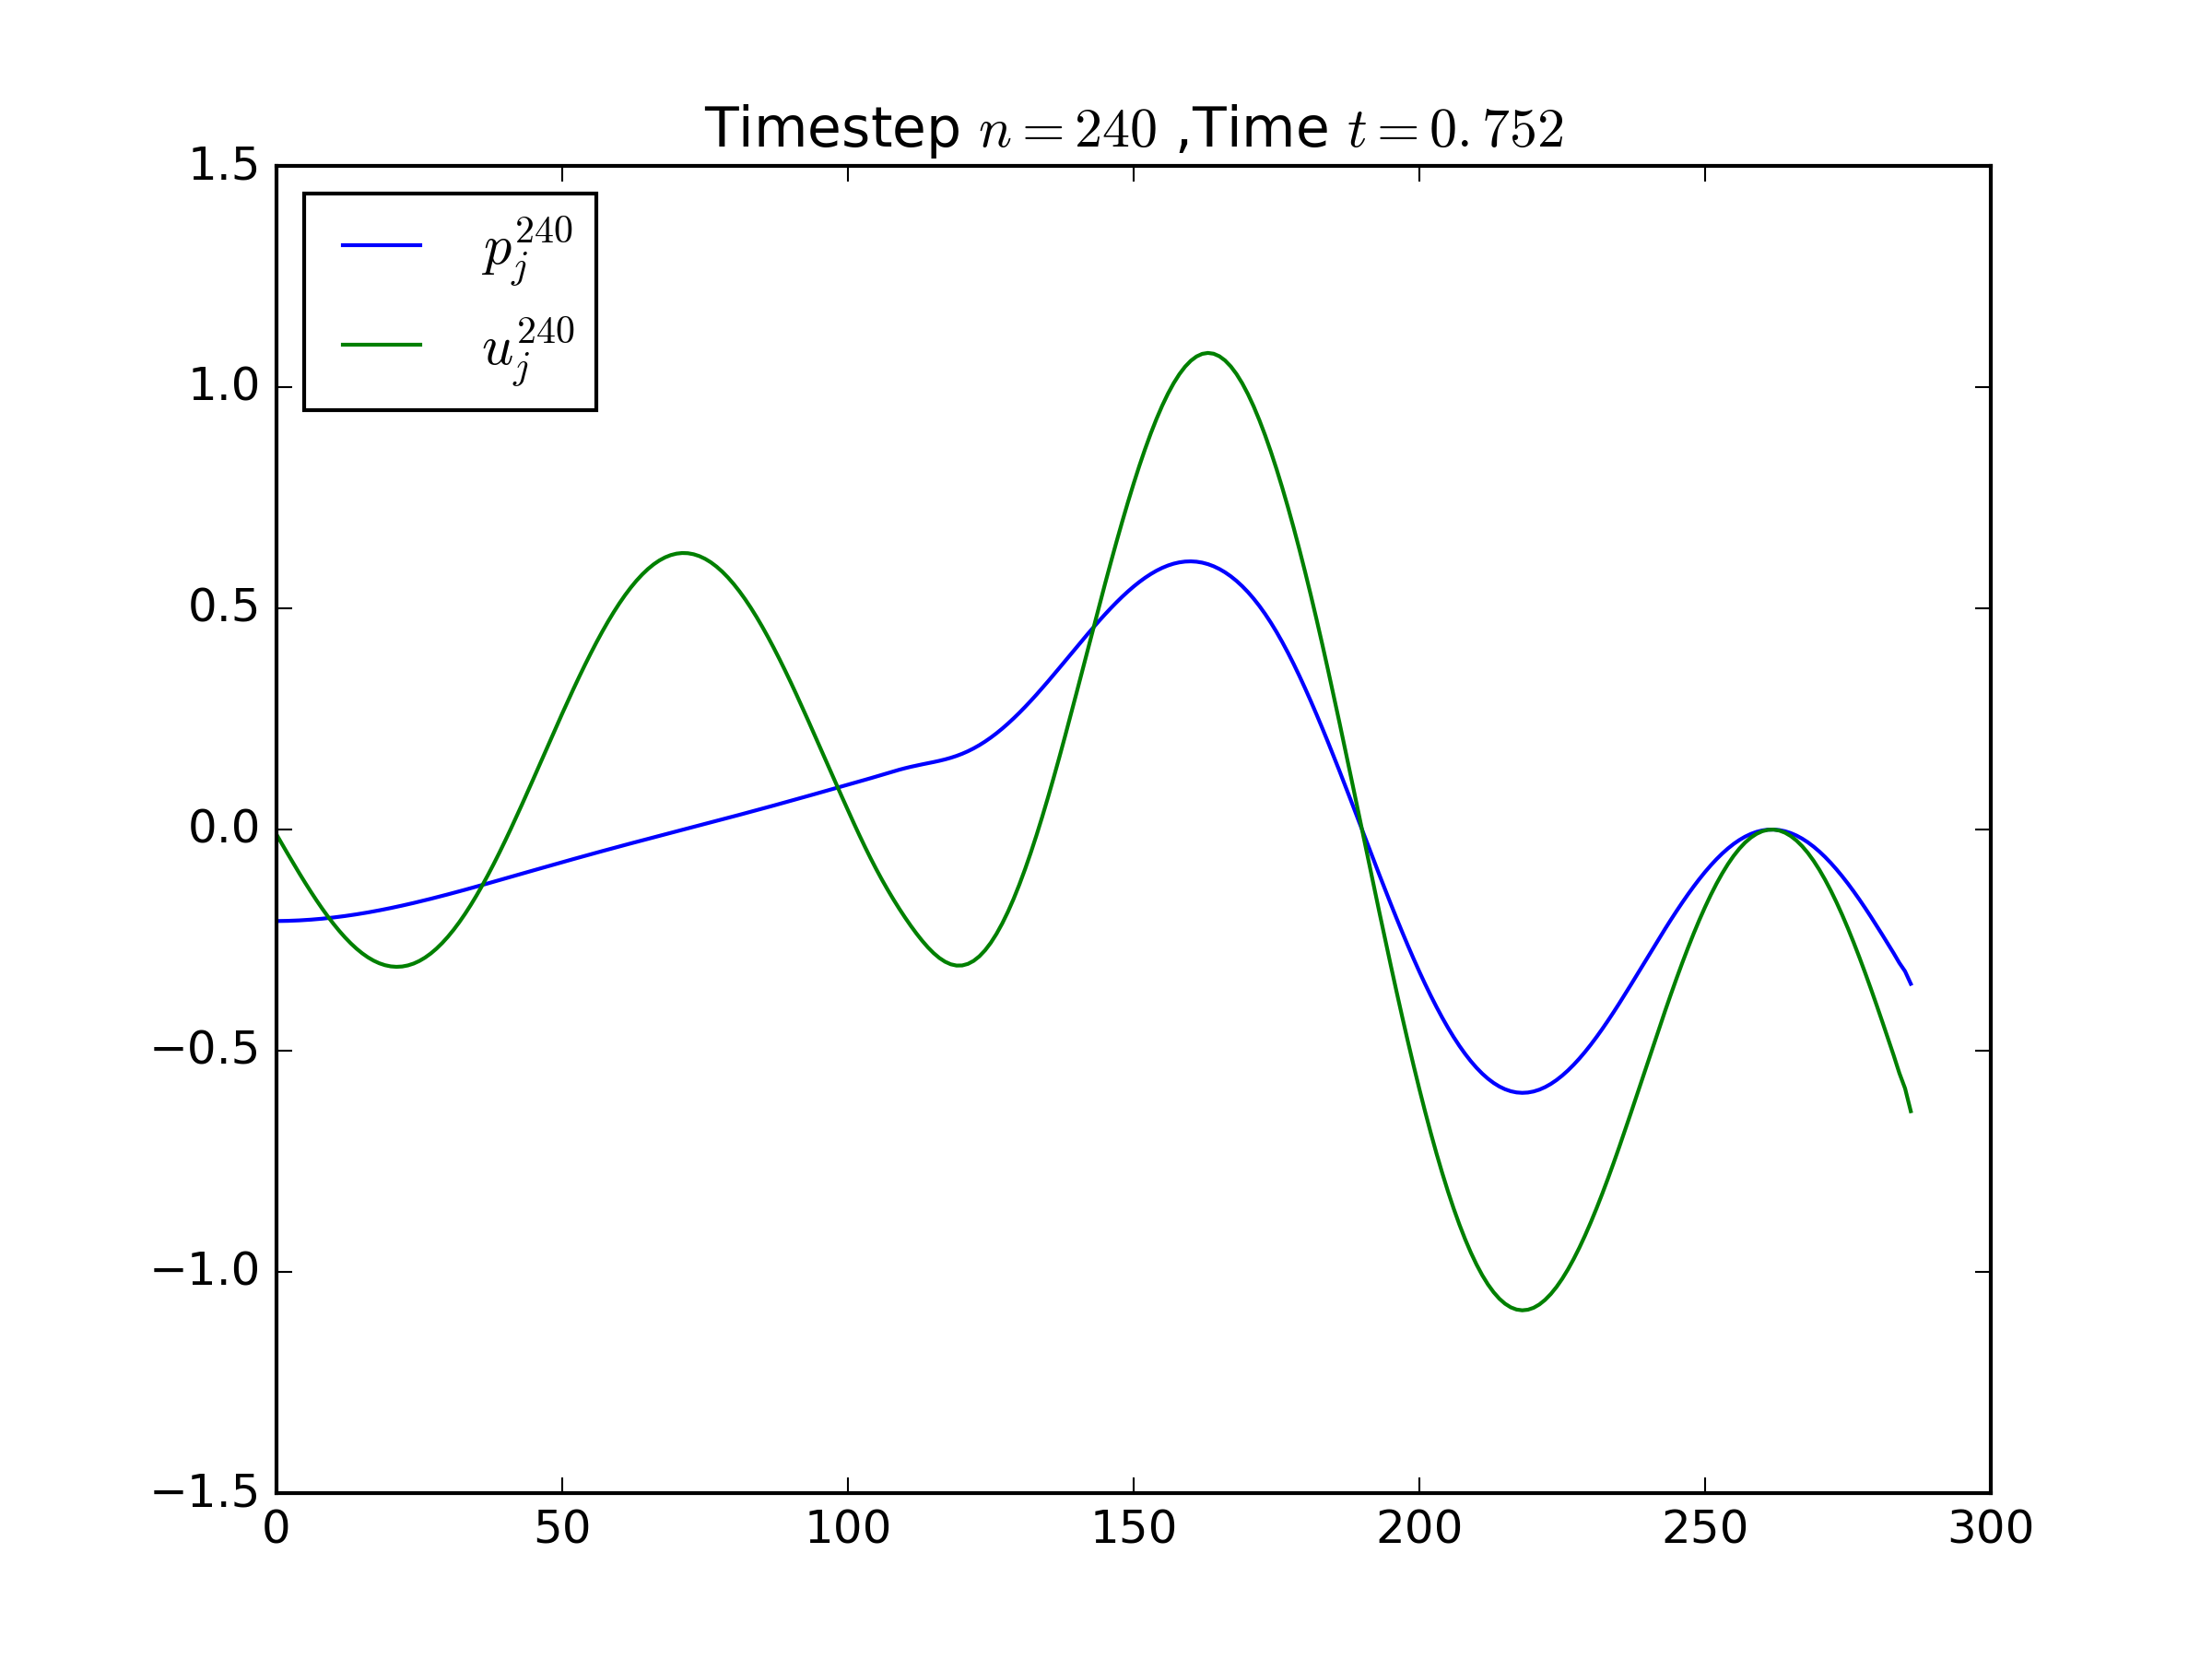
\includegraphics[width=0.31\textwidth]{figures/problem_1_c_024.png}
            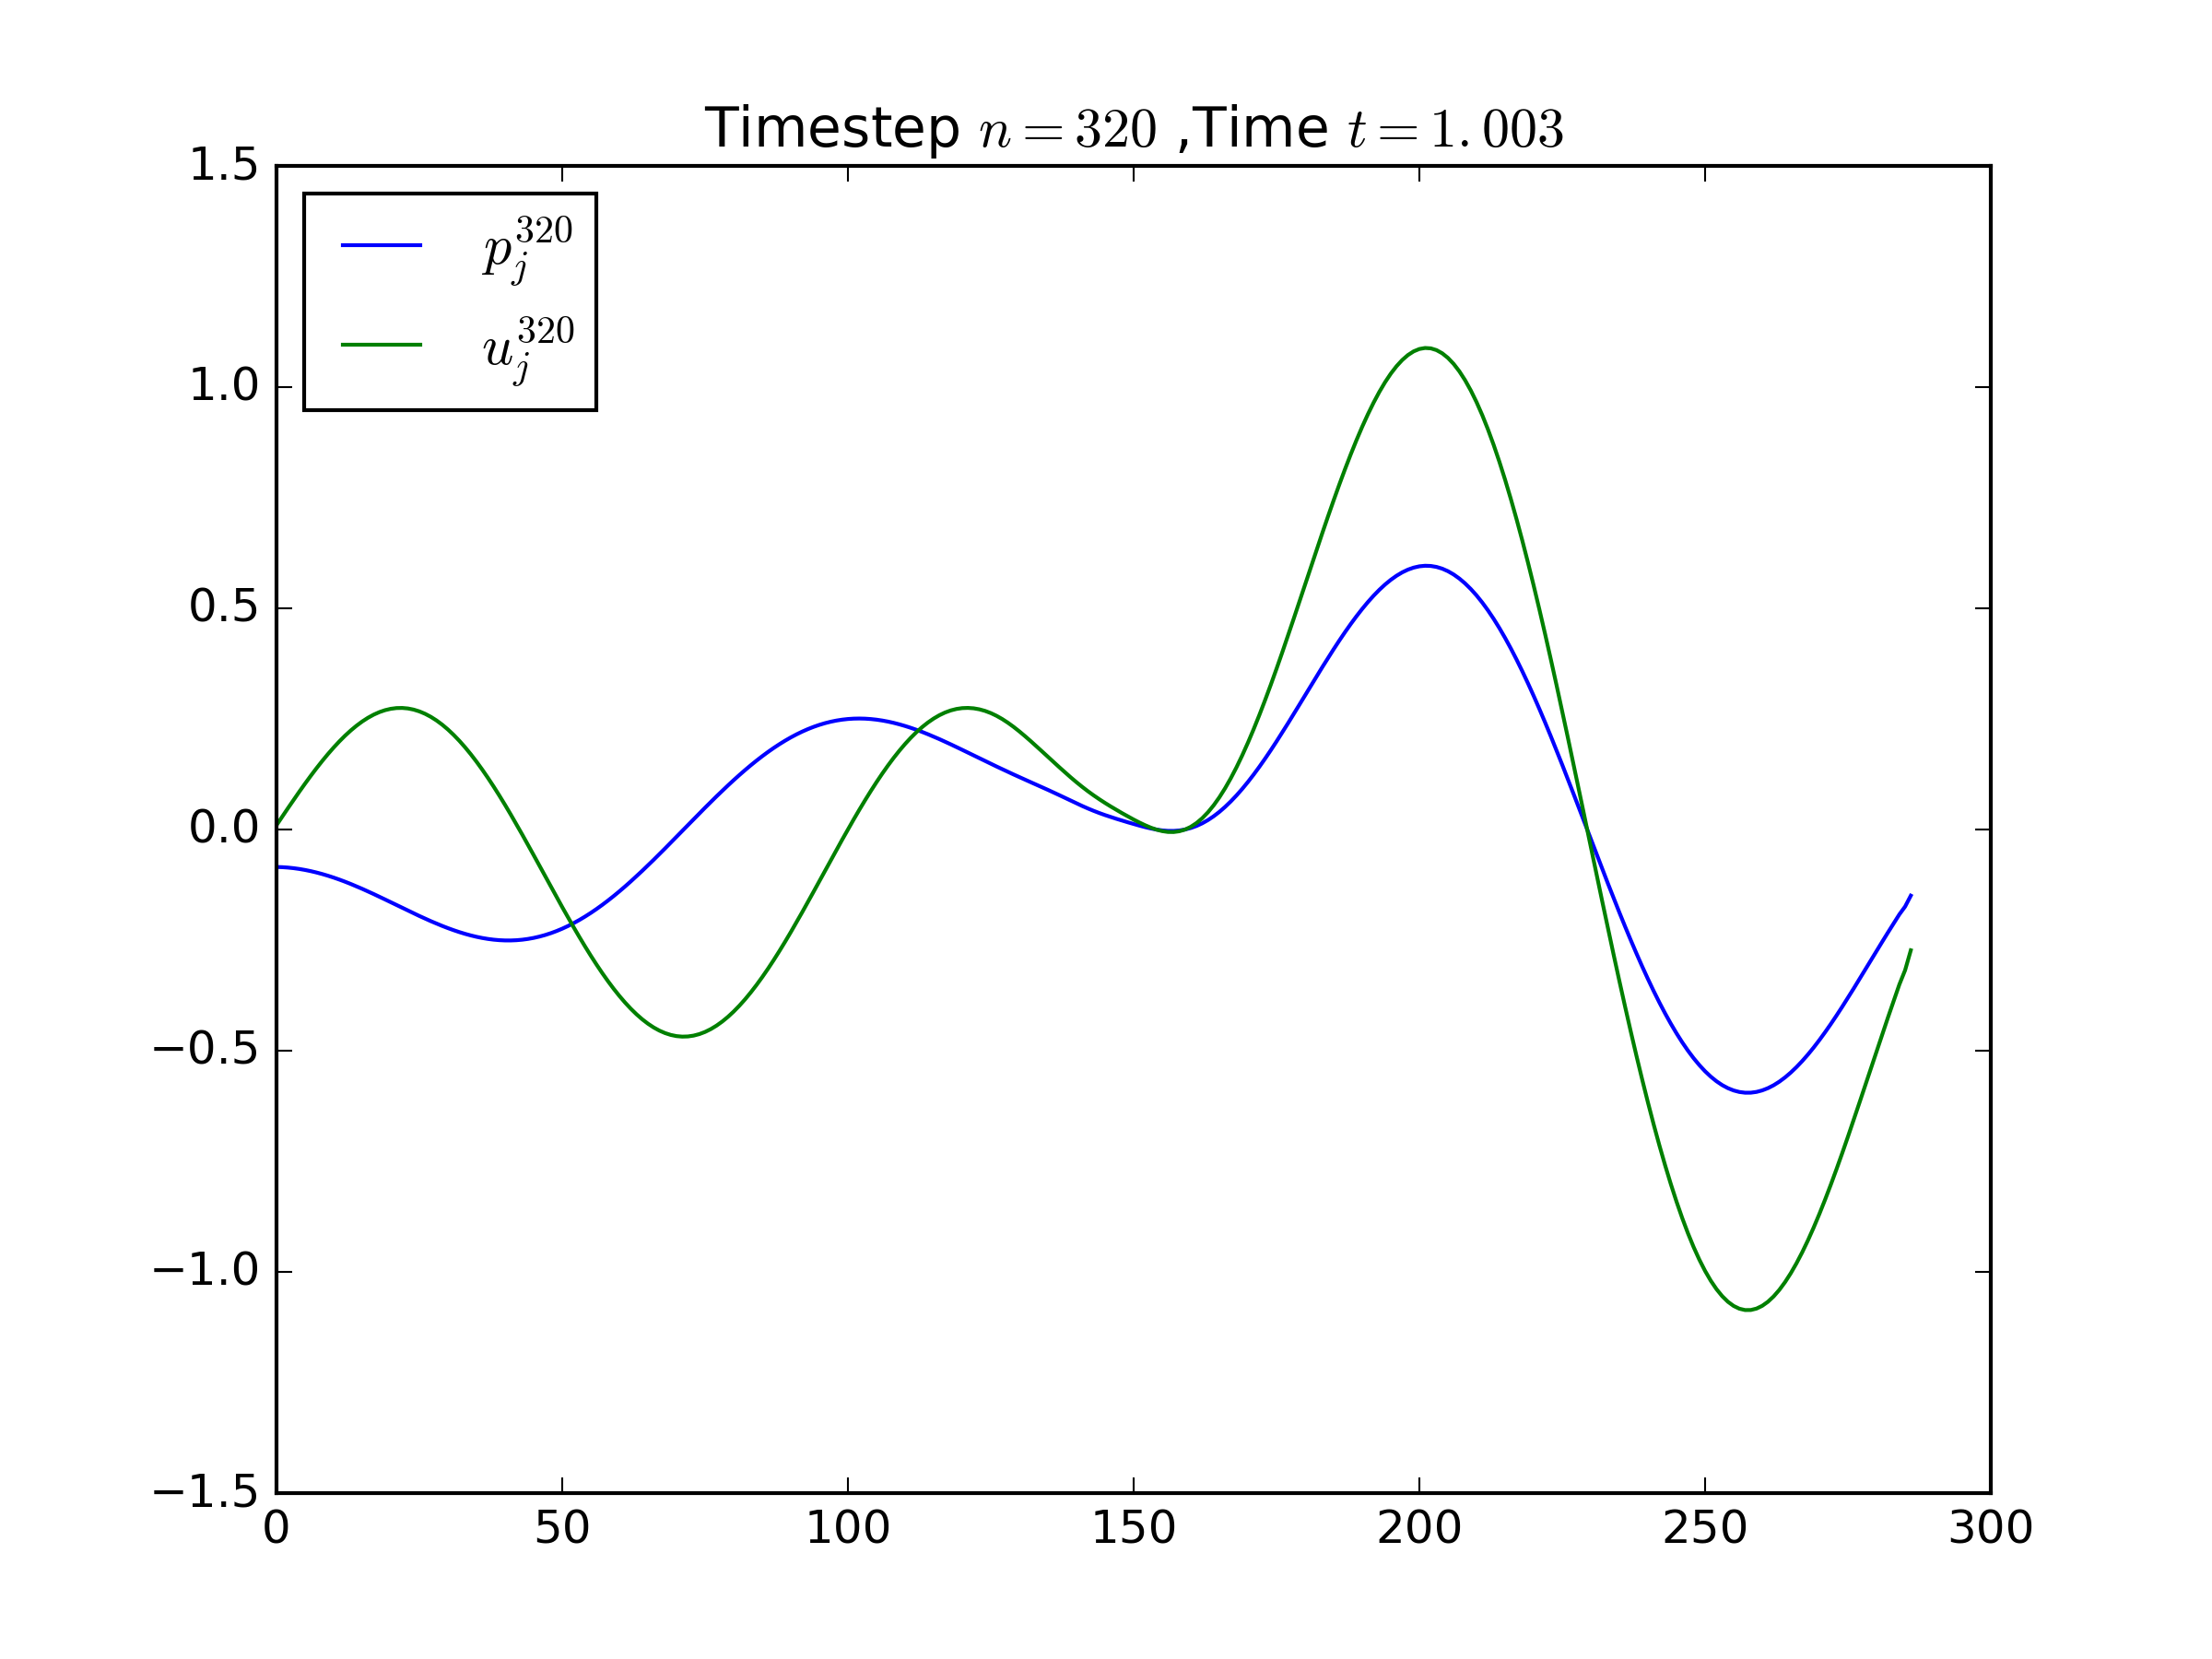
\includegraphics[width=0.31\textwidth]{figures/problem_1_c_032.png}
            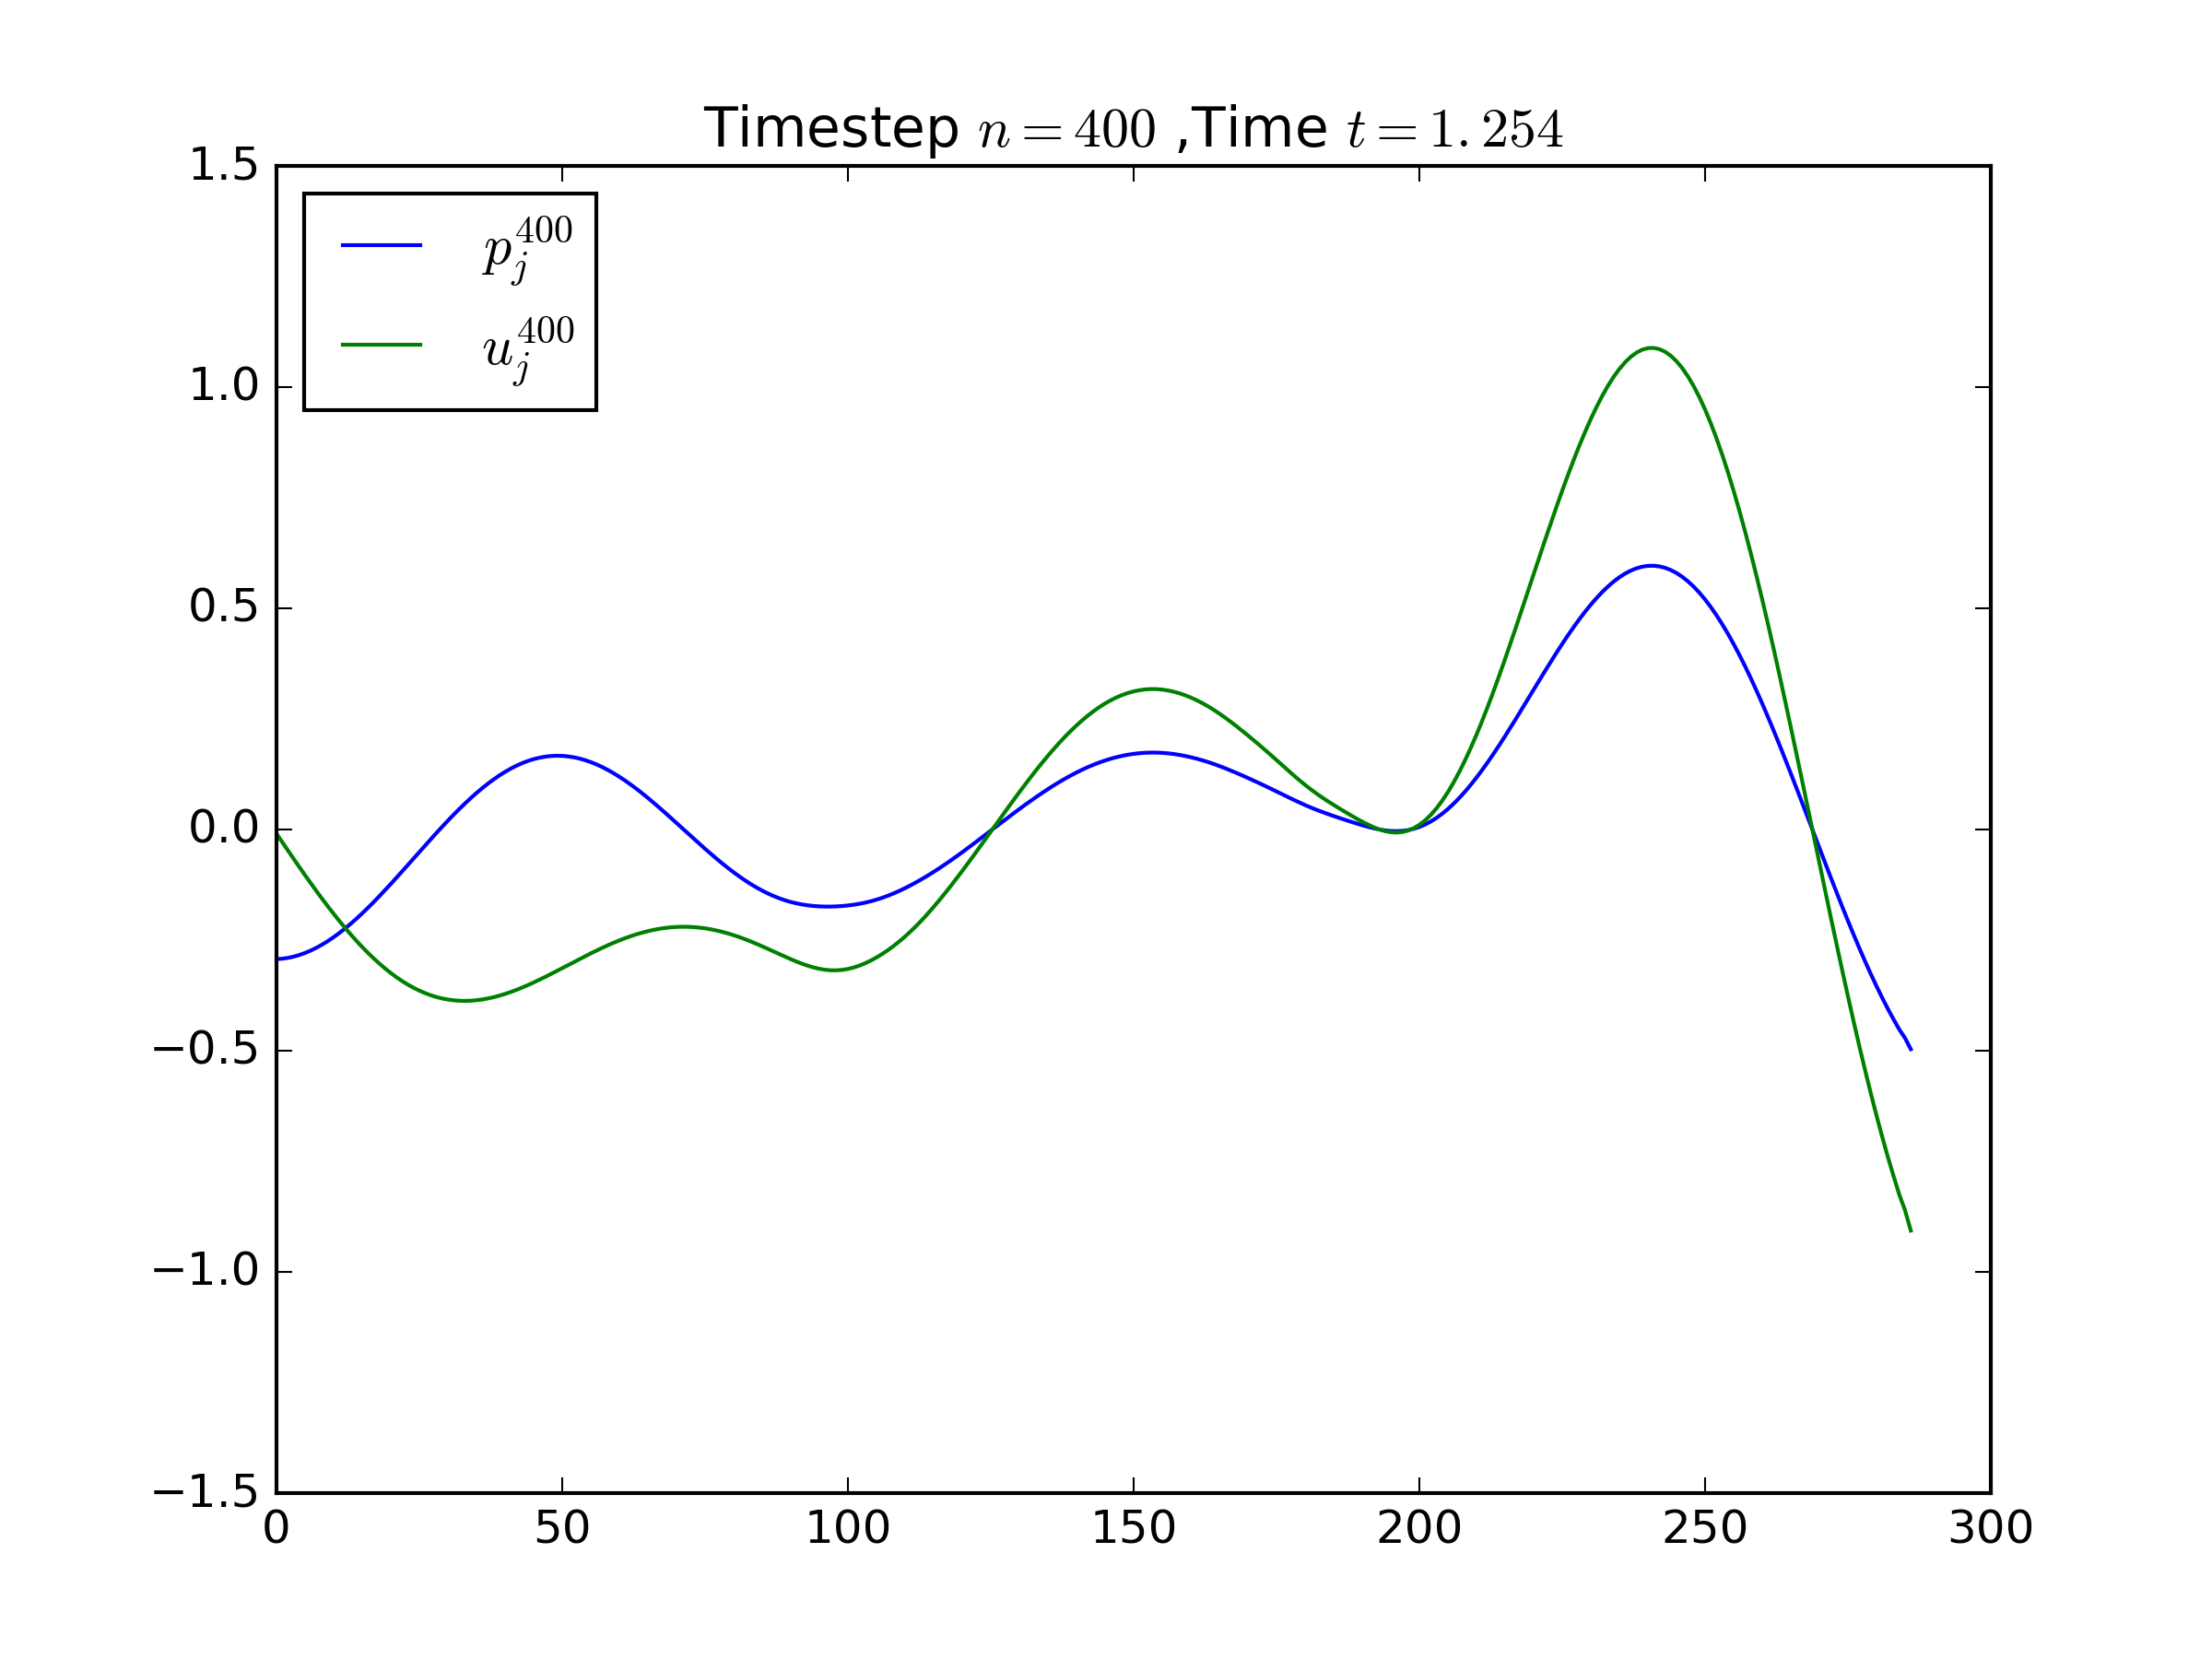
\includegraphics[width=0.31\textwidth]{figures/problem_1_c_040.png}
            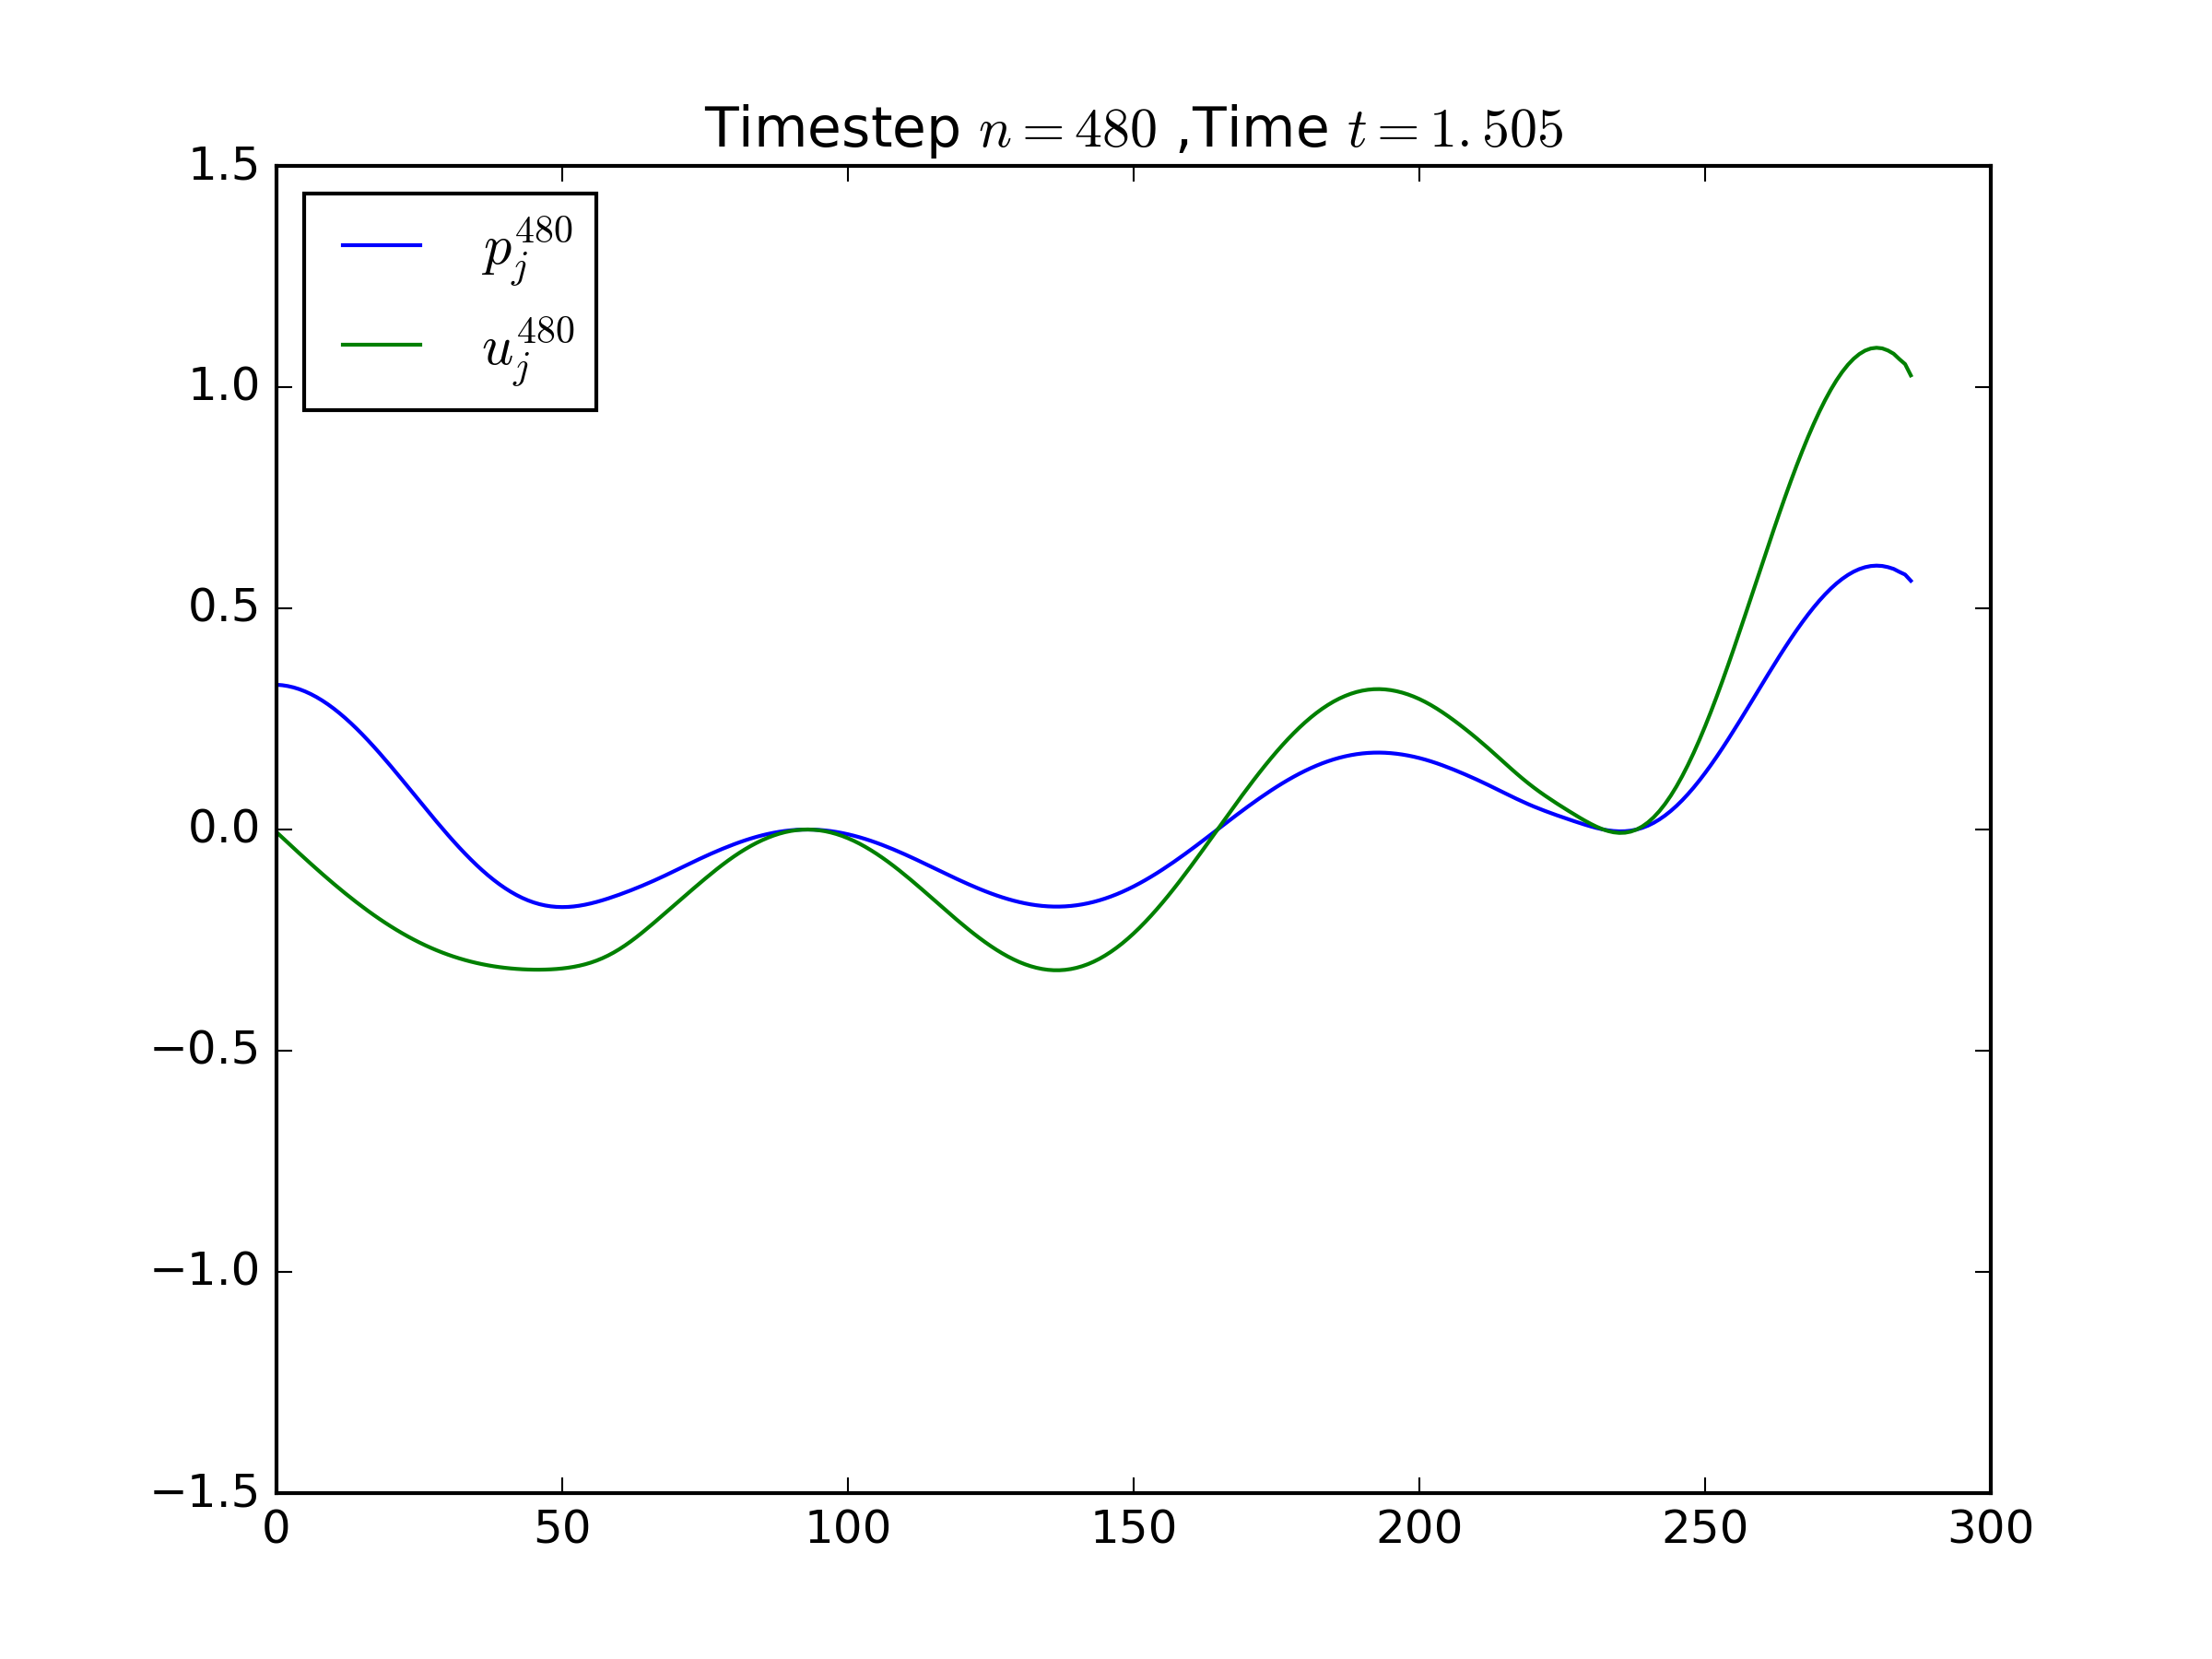
\includegraphics[width=0.31\textwidth]{figures/problem_1_c_048.png}
            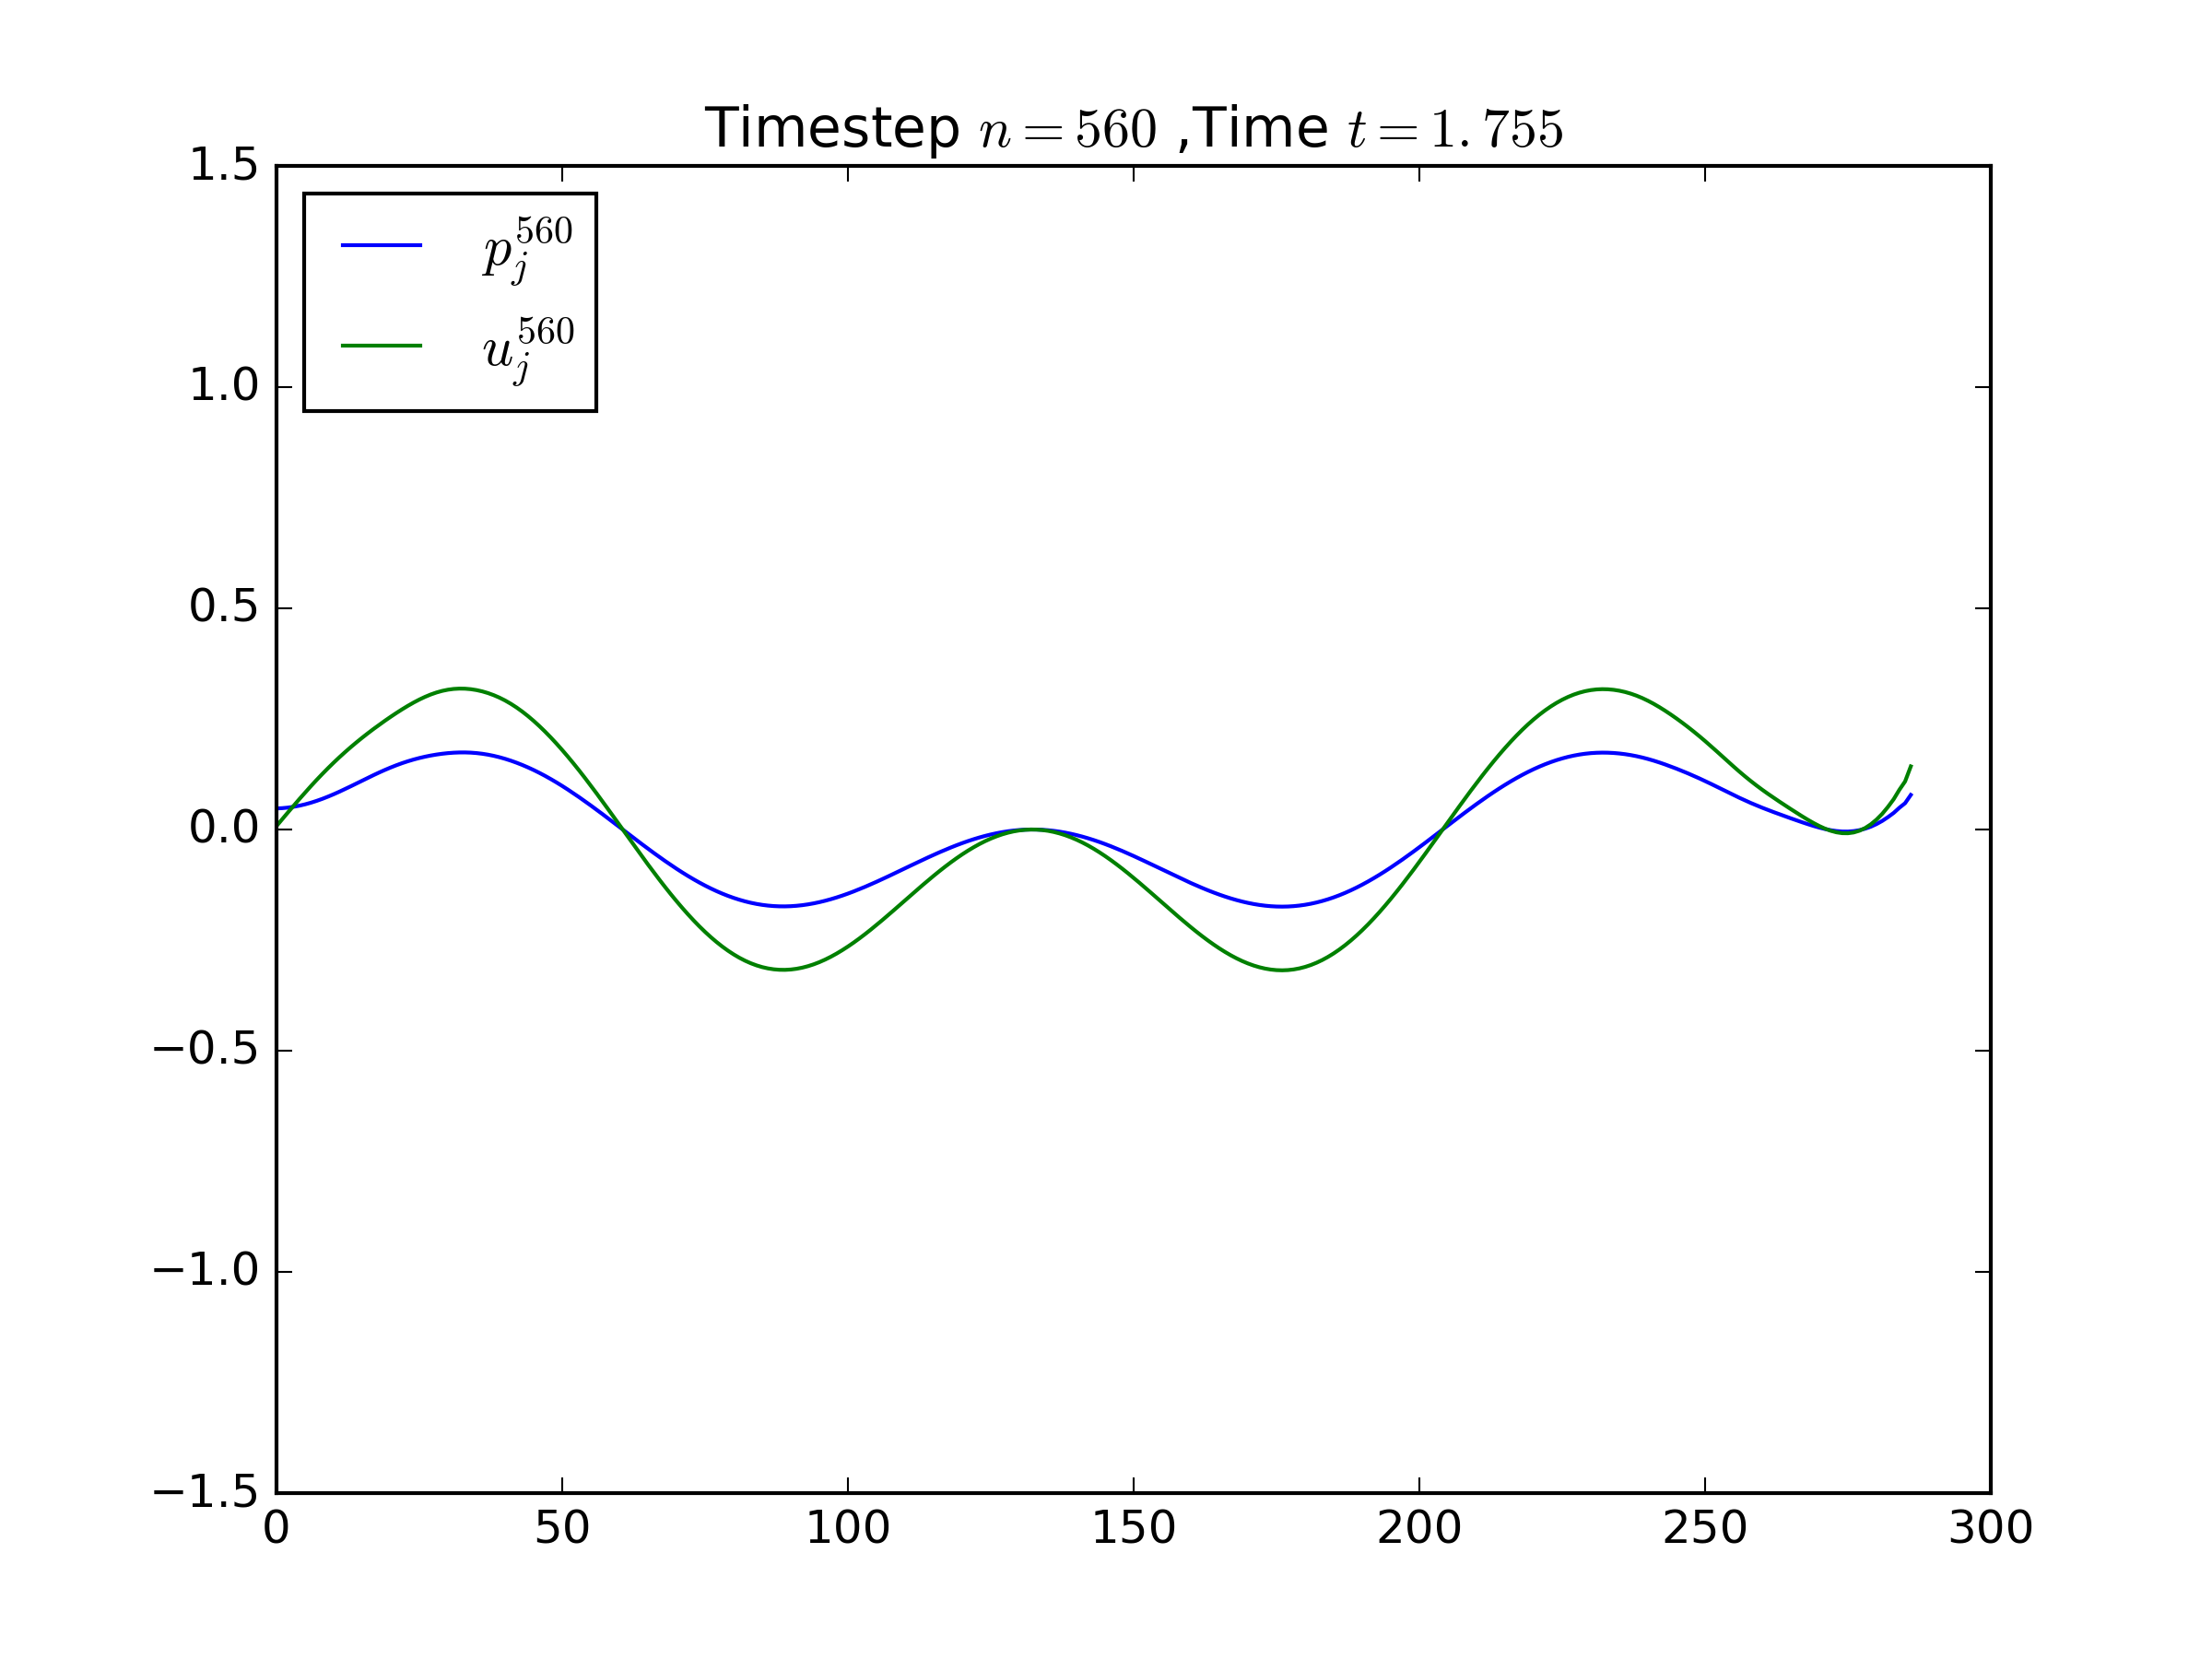
\includegraphics[width=0.31\textwidth]{figures/problem_1_c_056.png}
            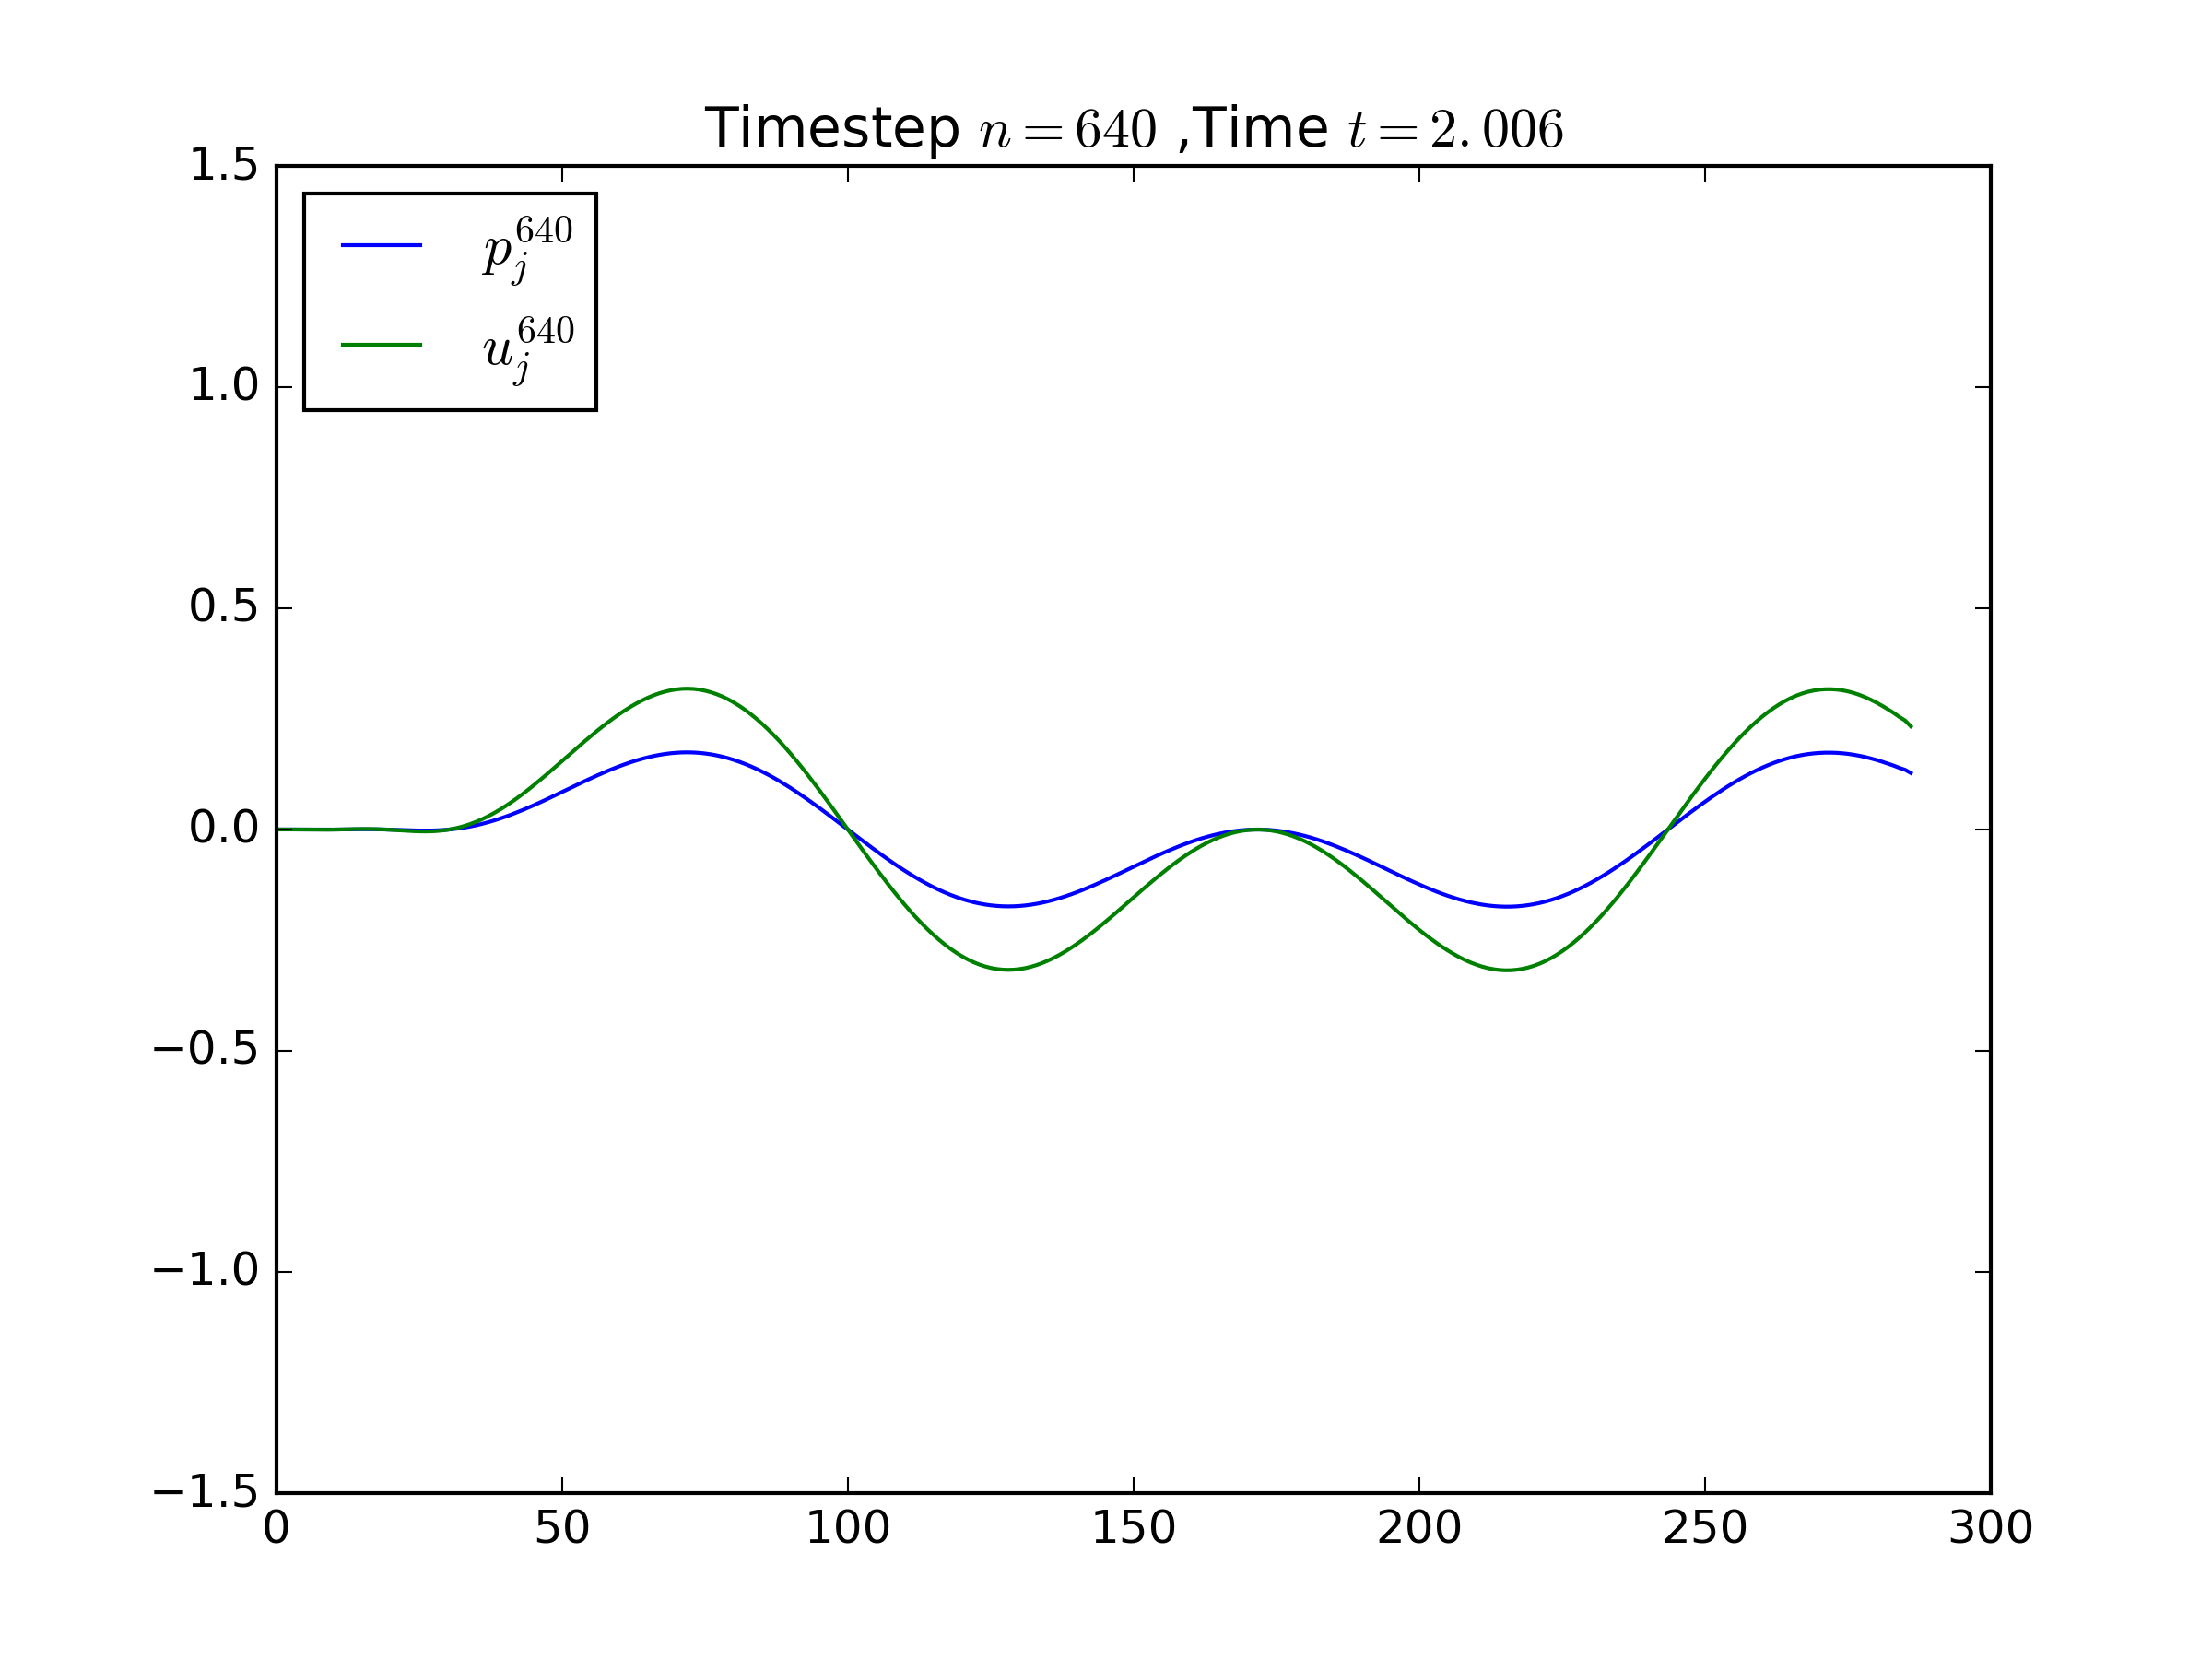
\includegraphics[width=0.31\textwidth]{figures/problem_1_c_064.png}
            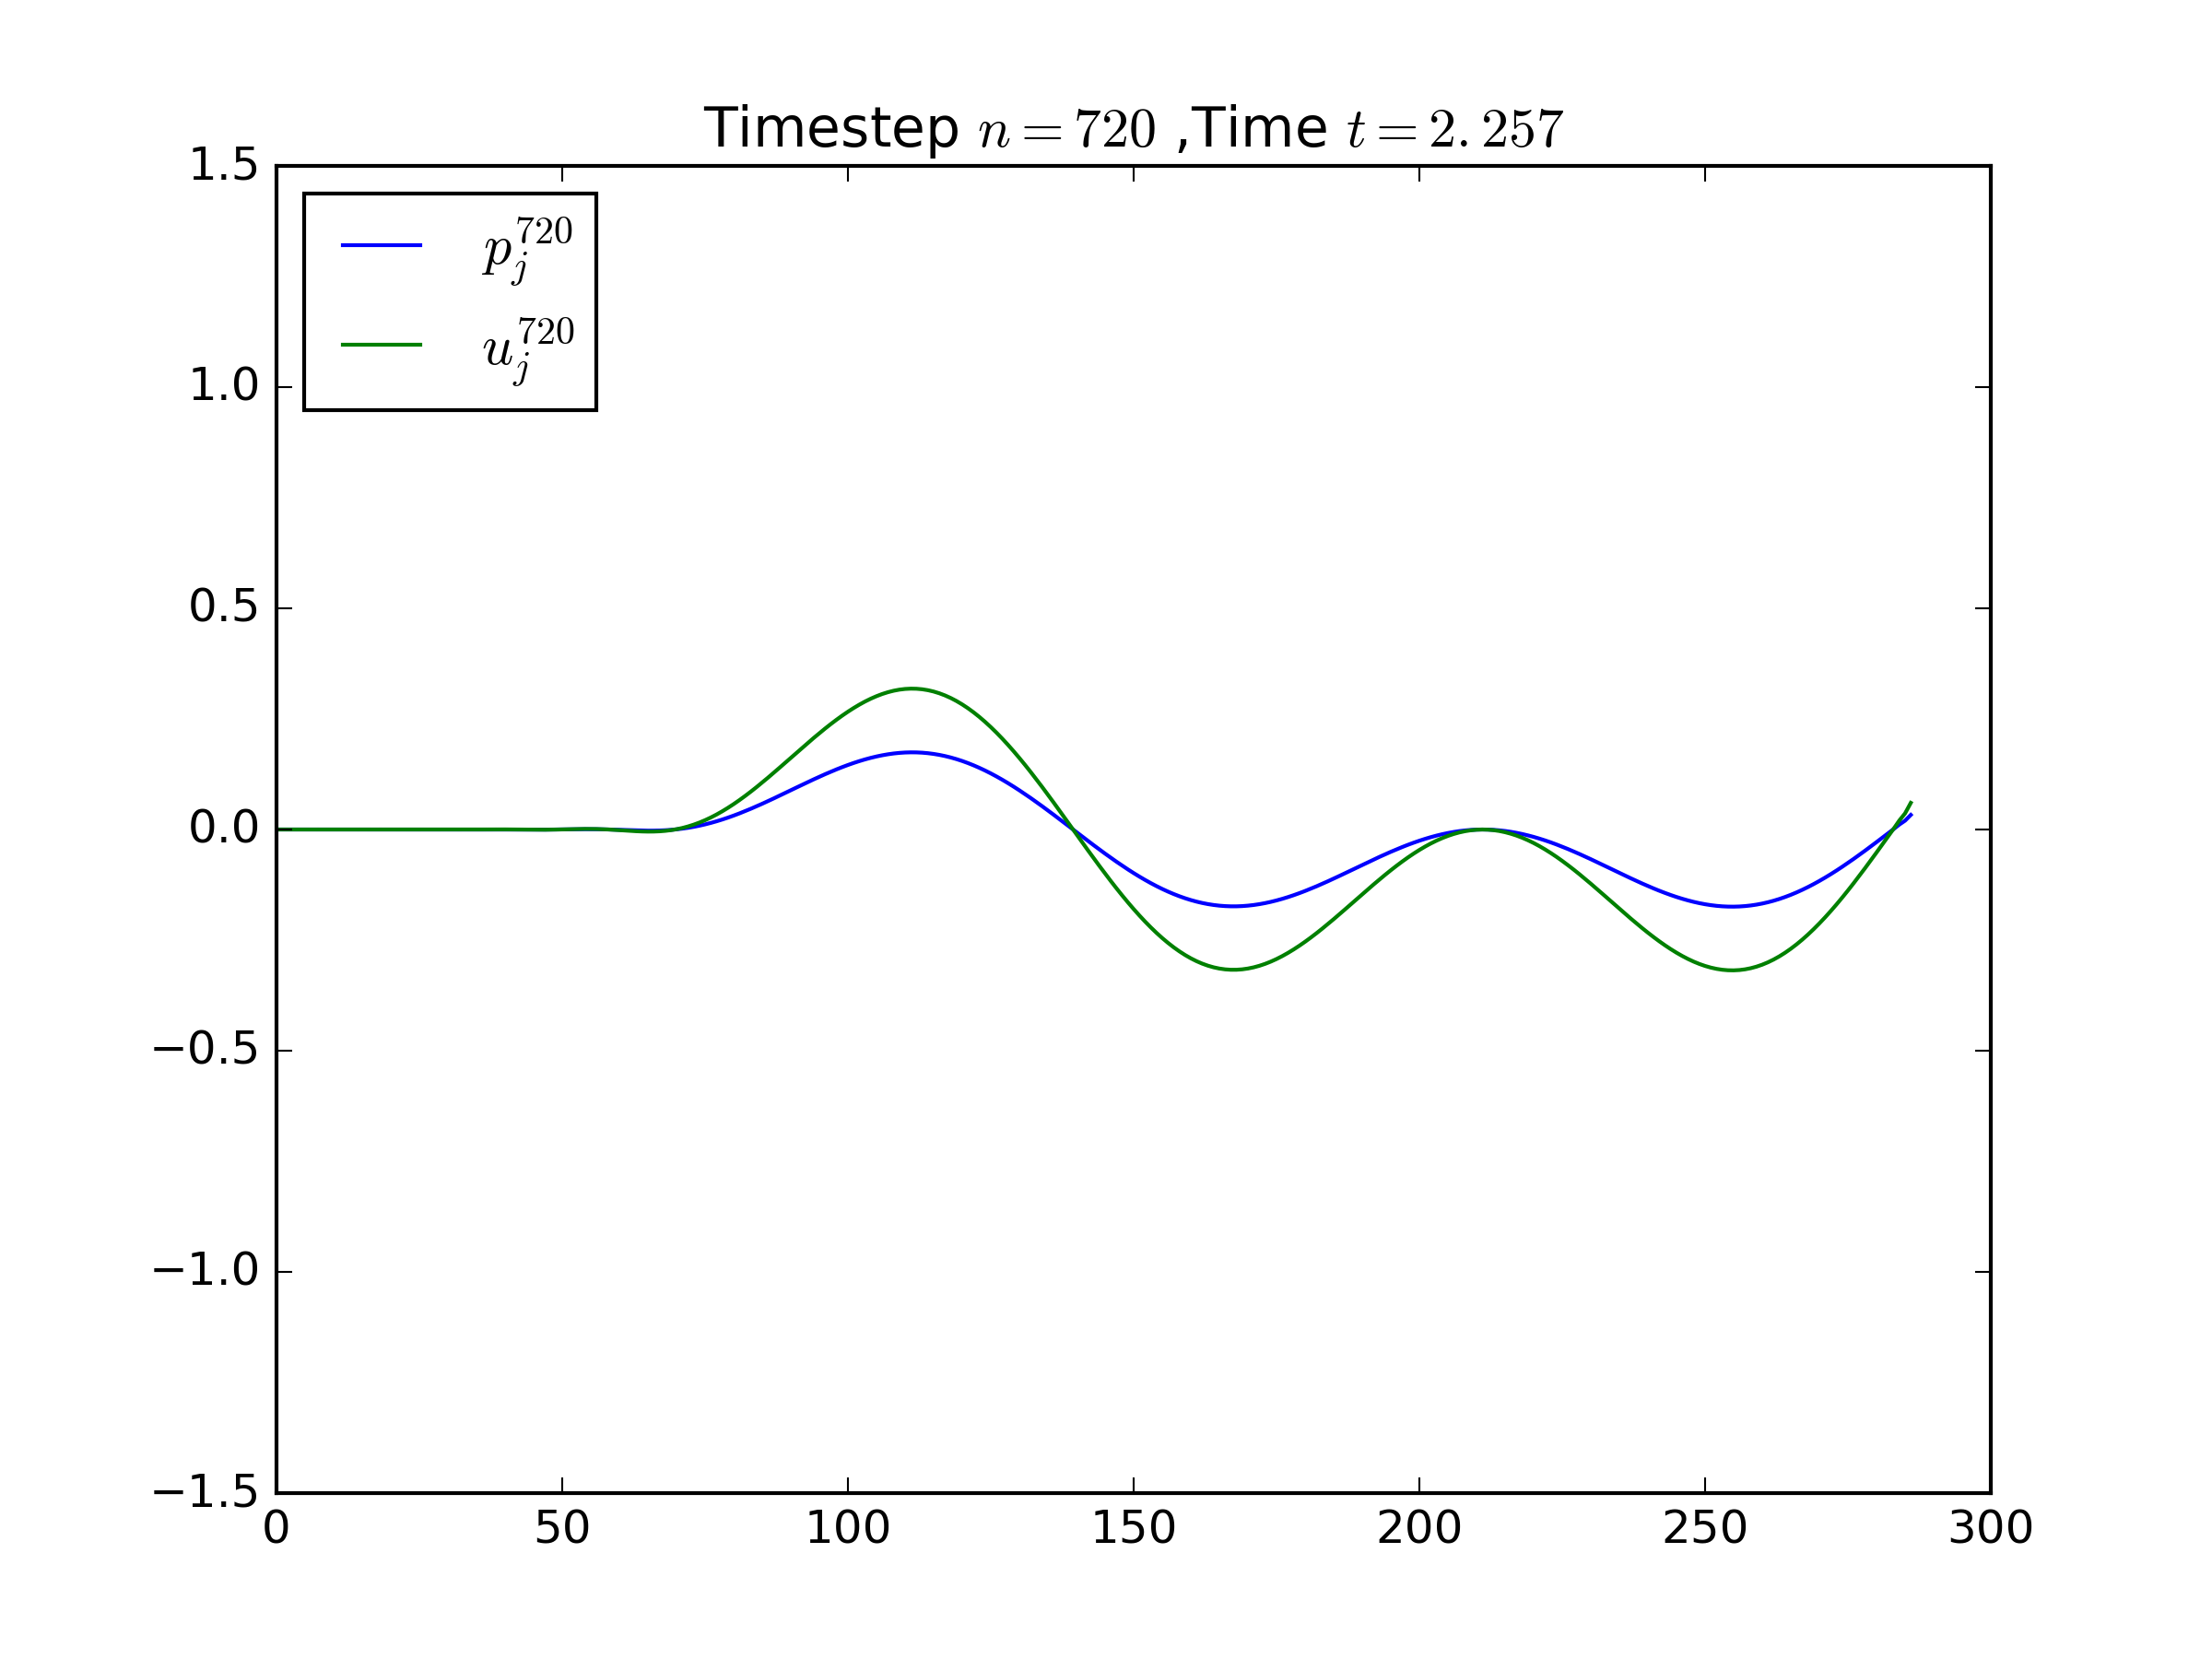
\includegraphics[width=0.31\textwidth]{figures/problem_1_c_072.png}
            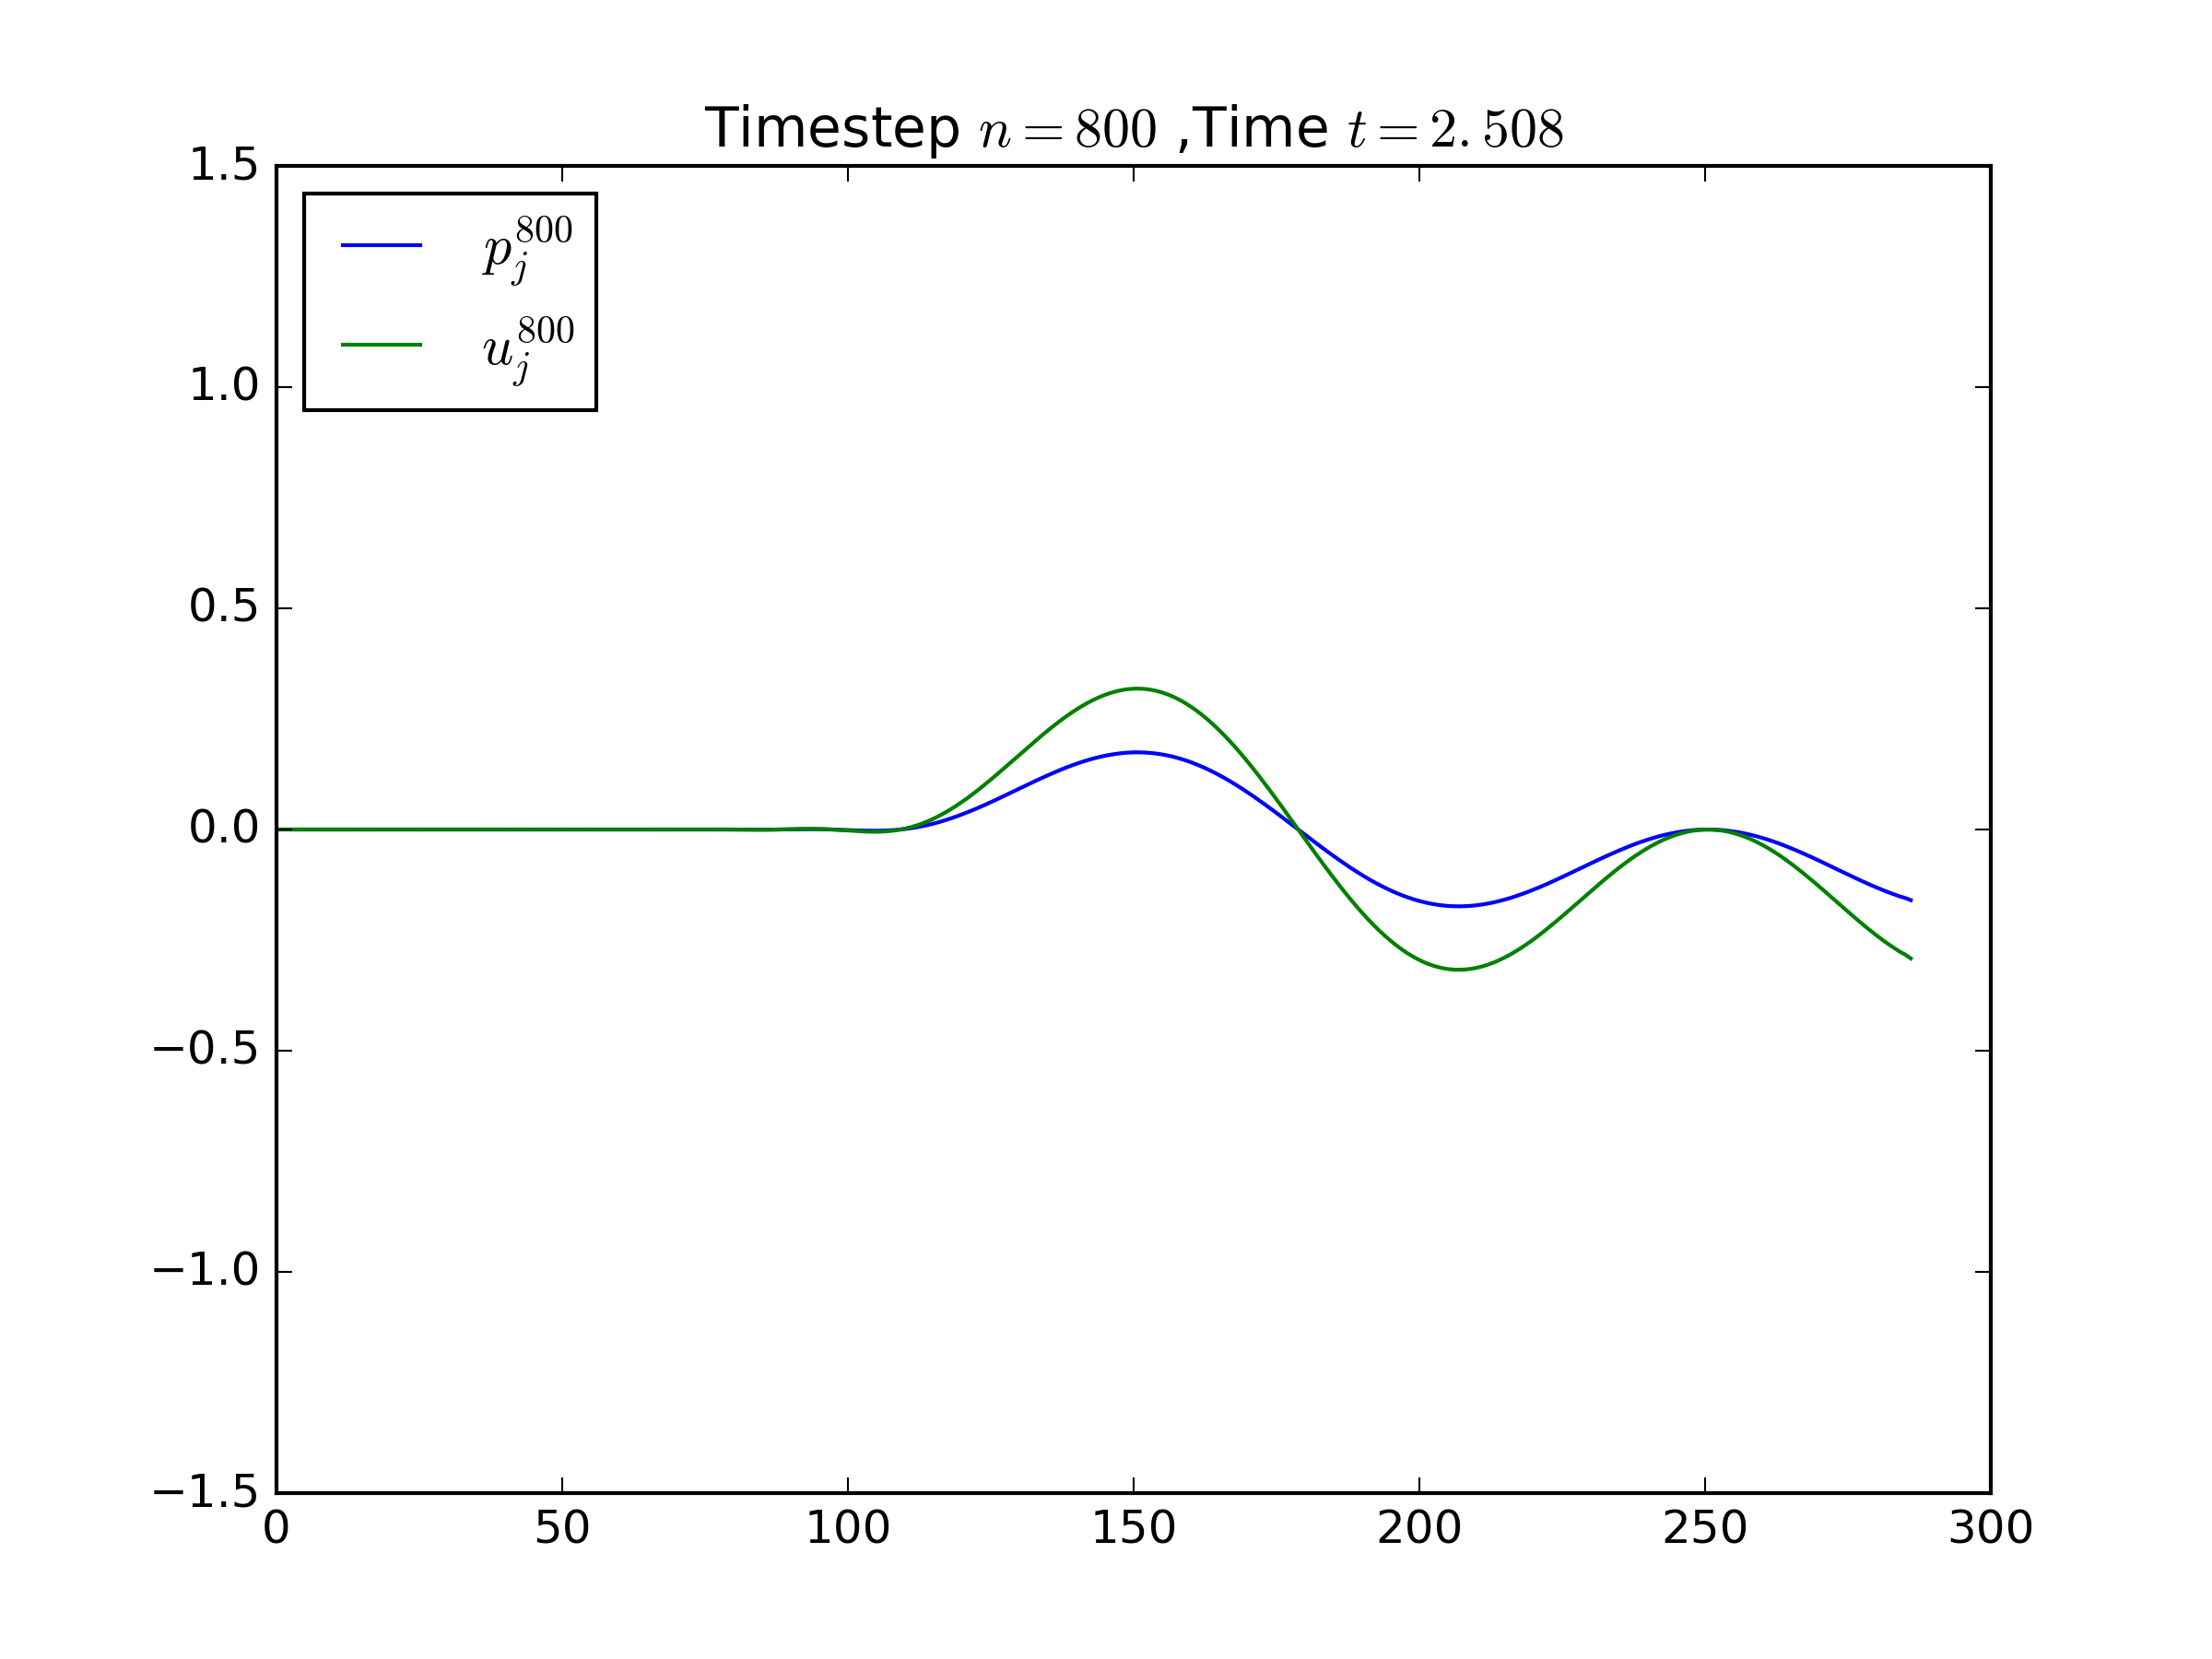
\includegraphics[width=0.31\textwidth]{figures/problem_1_c_080.png}
            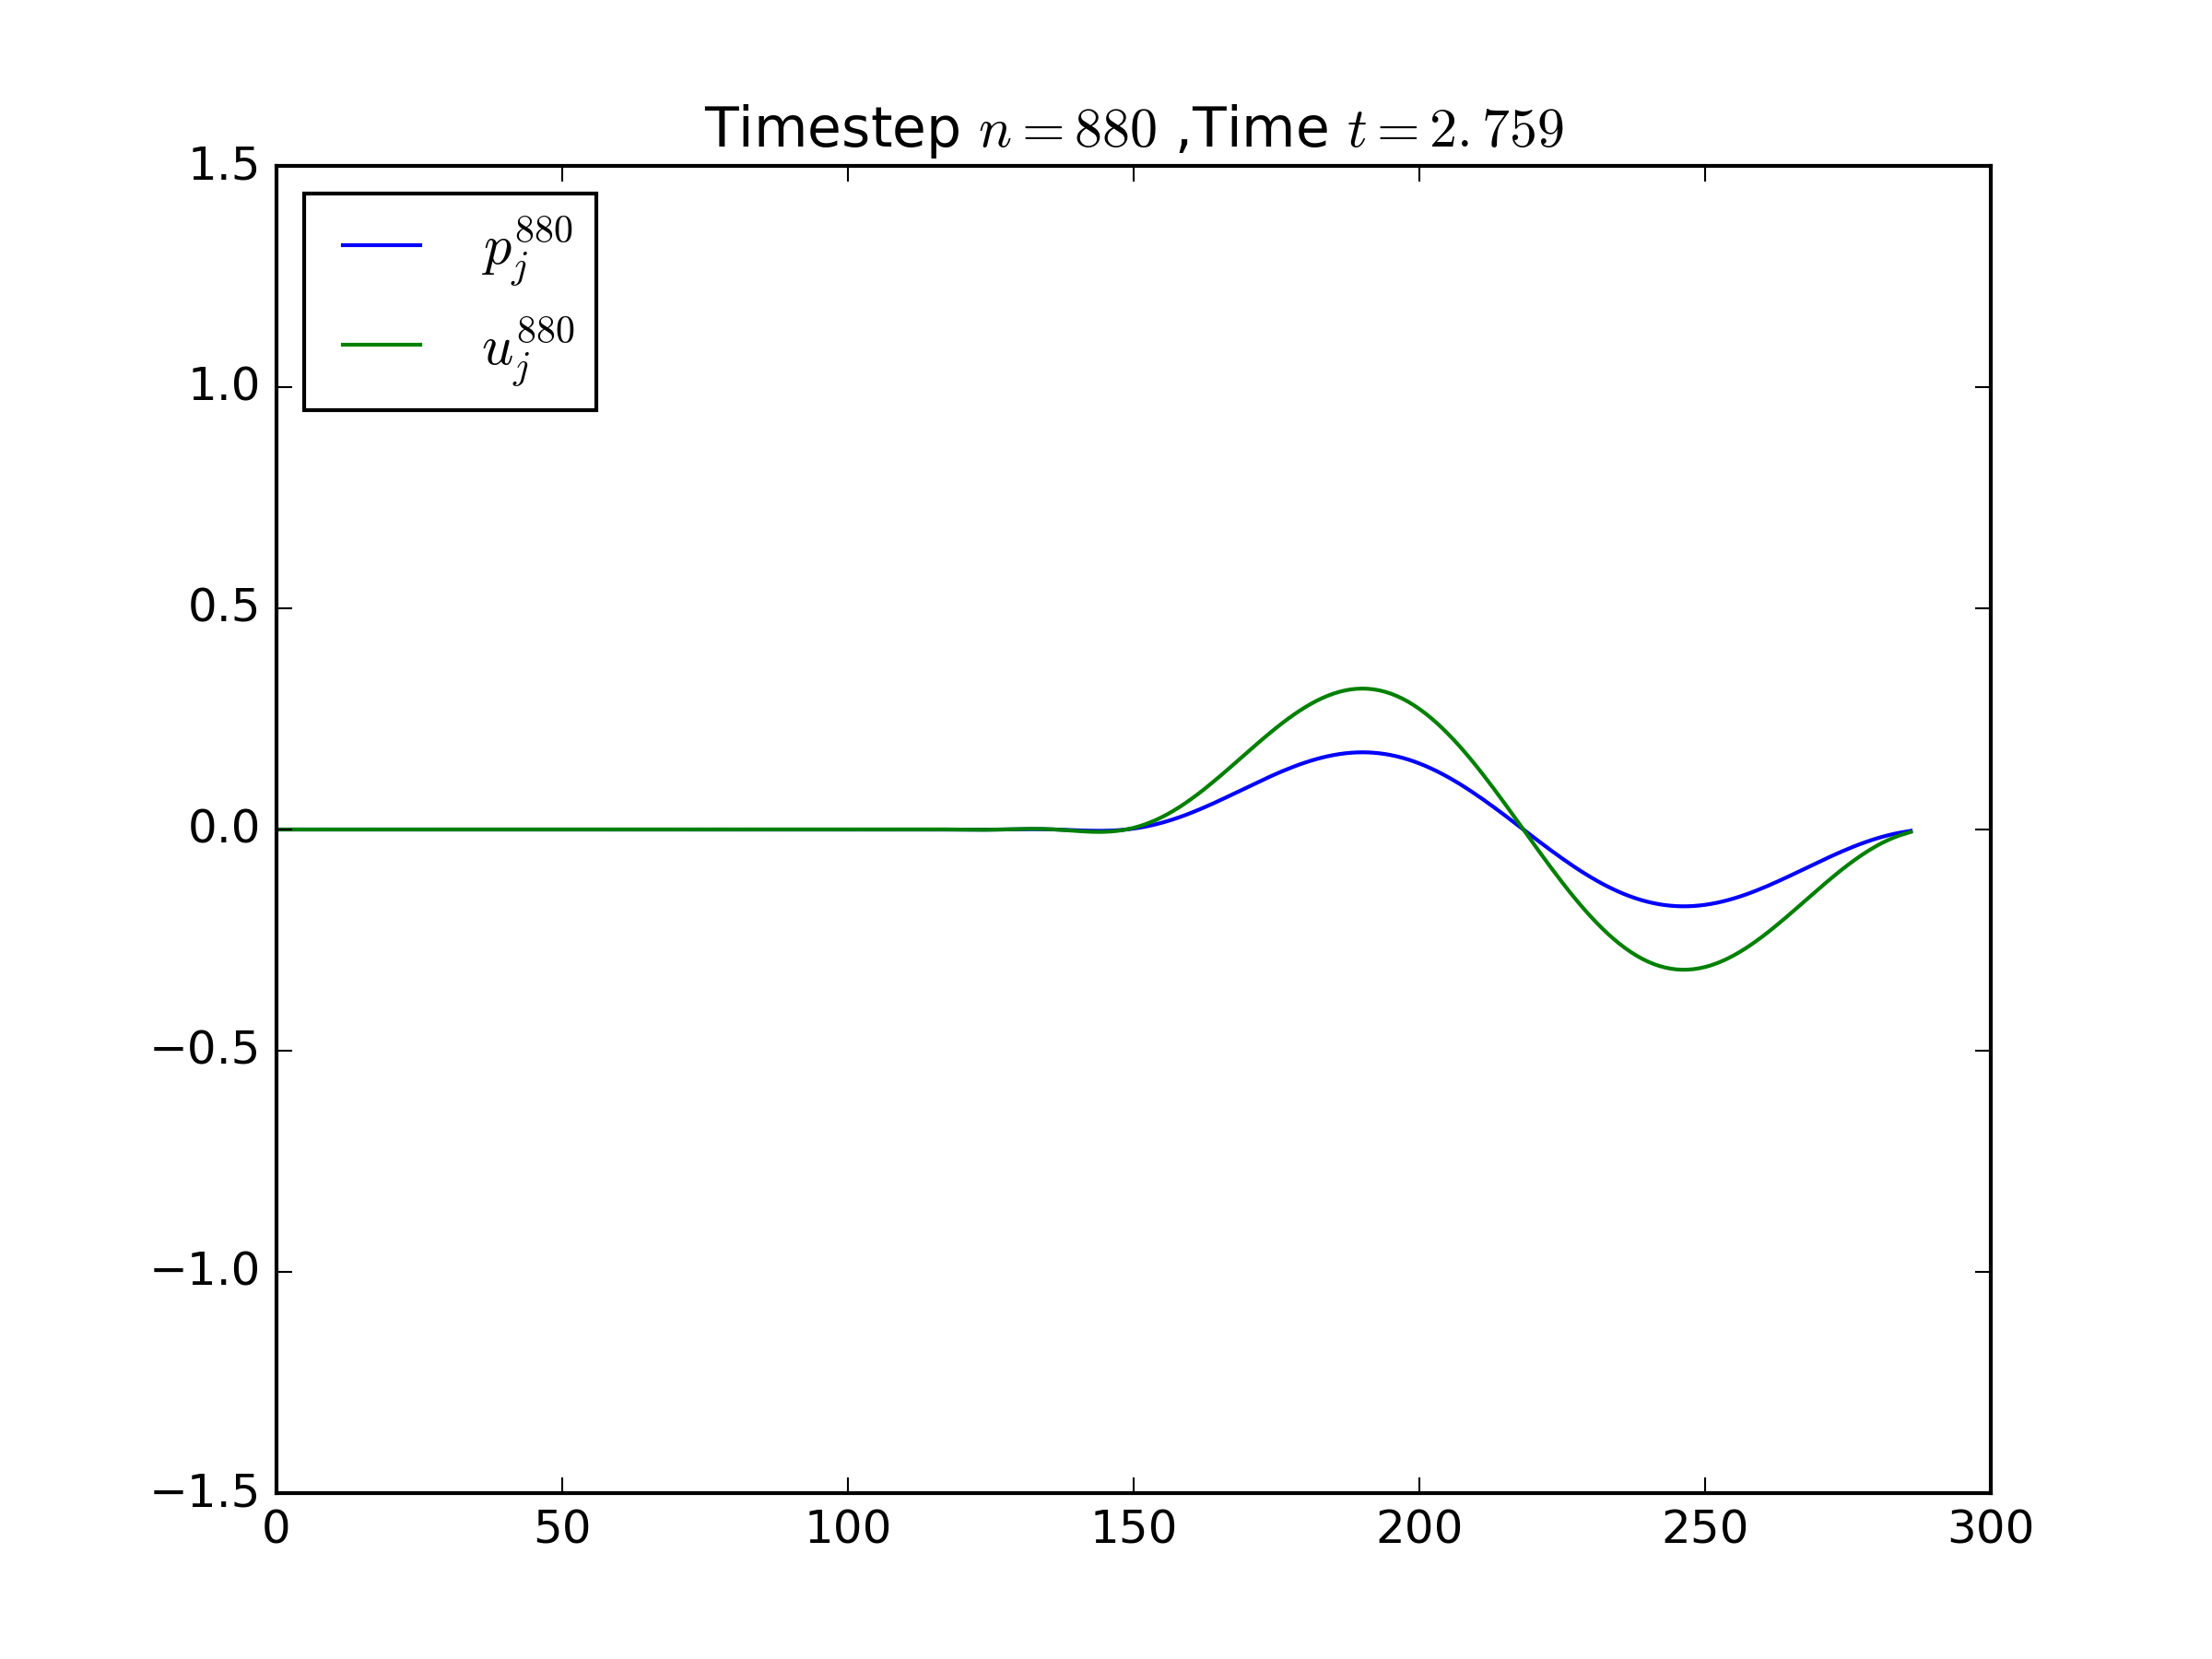
\includegraphics[width=0.31\textwidth]{figures/problem_1_c_088.png}
            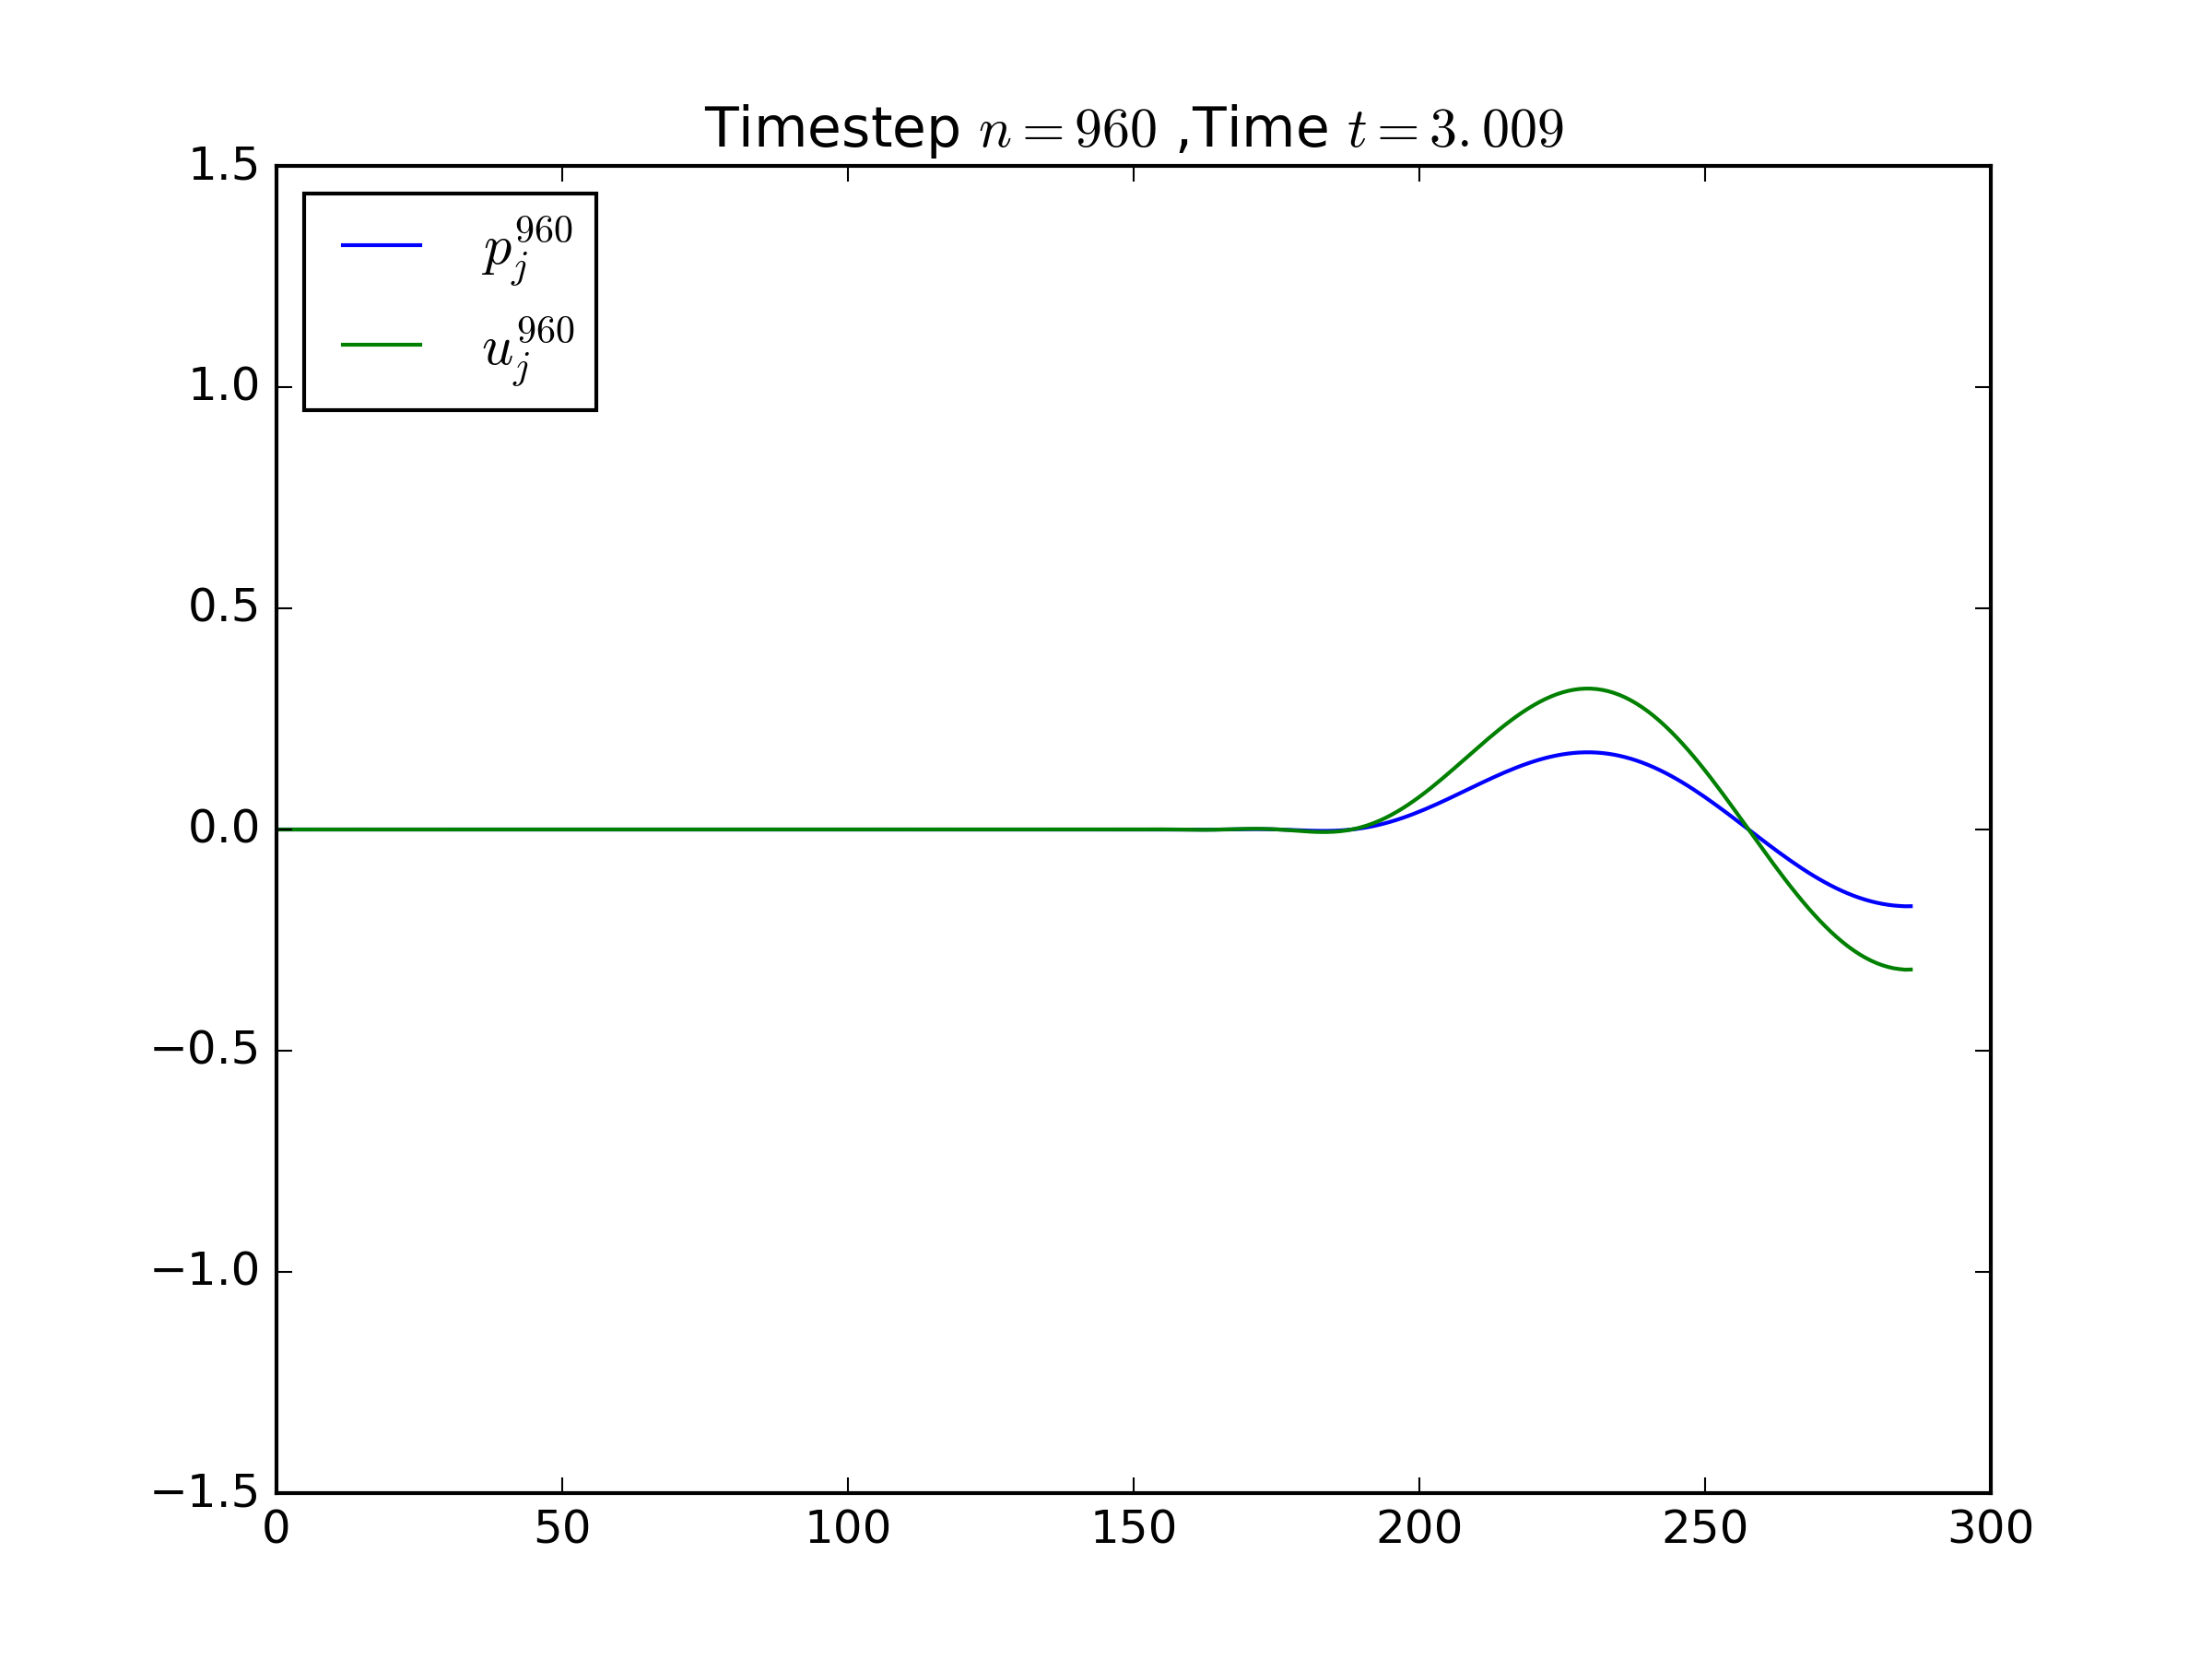
\includegraphics[width=0.31\textwidth]{figures/problem_1_c_096.png}
            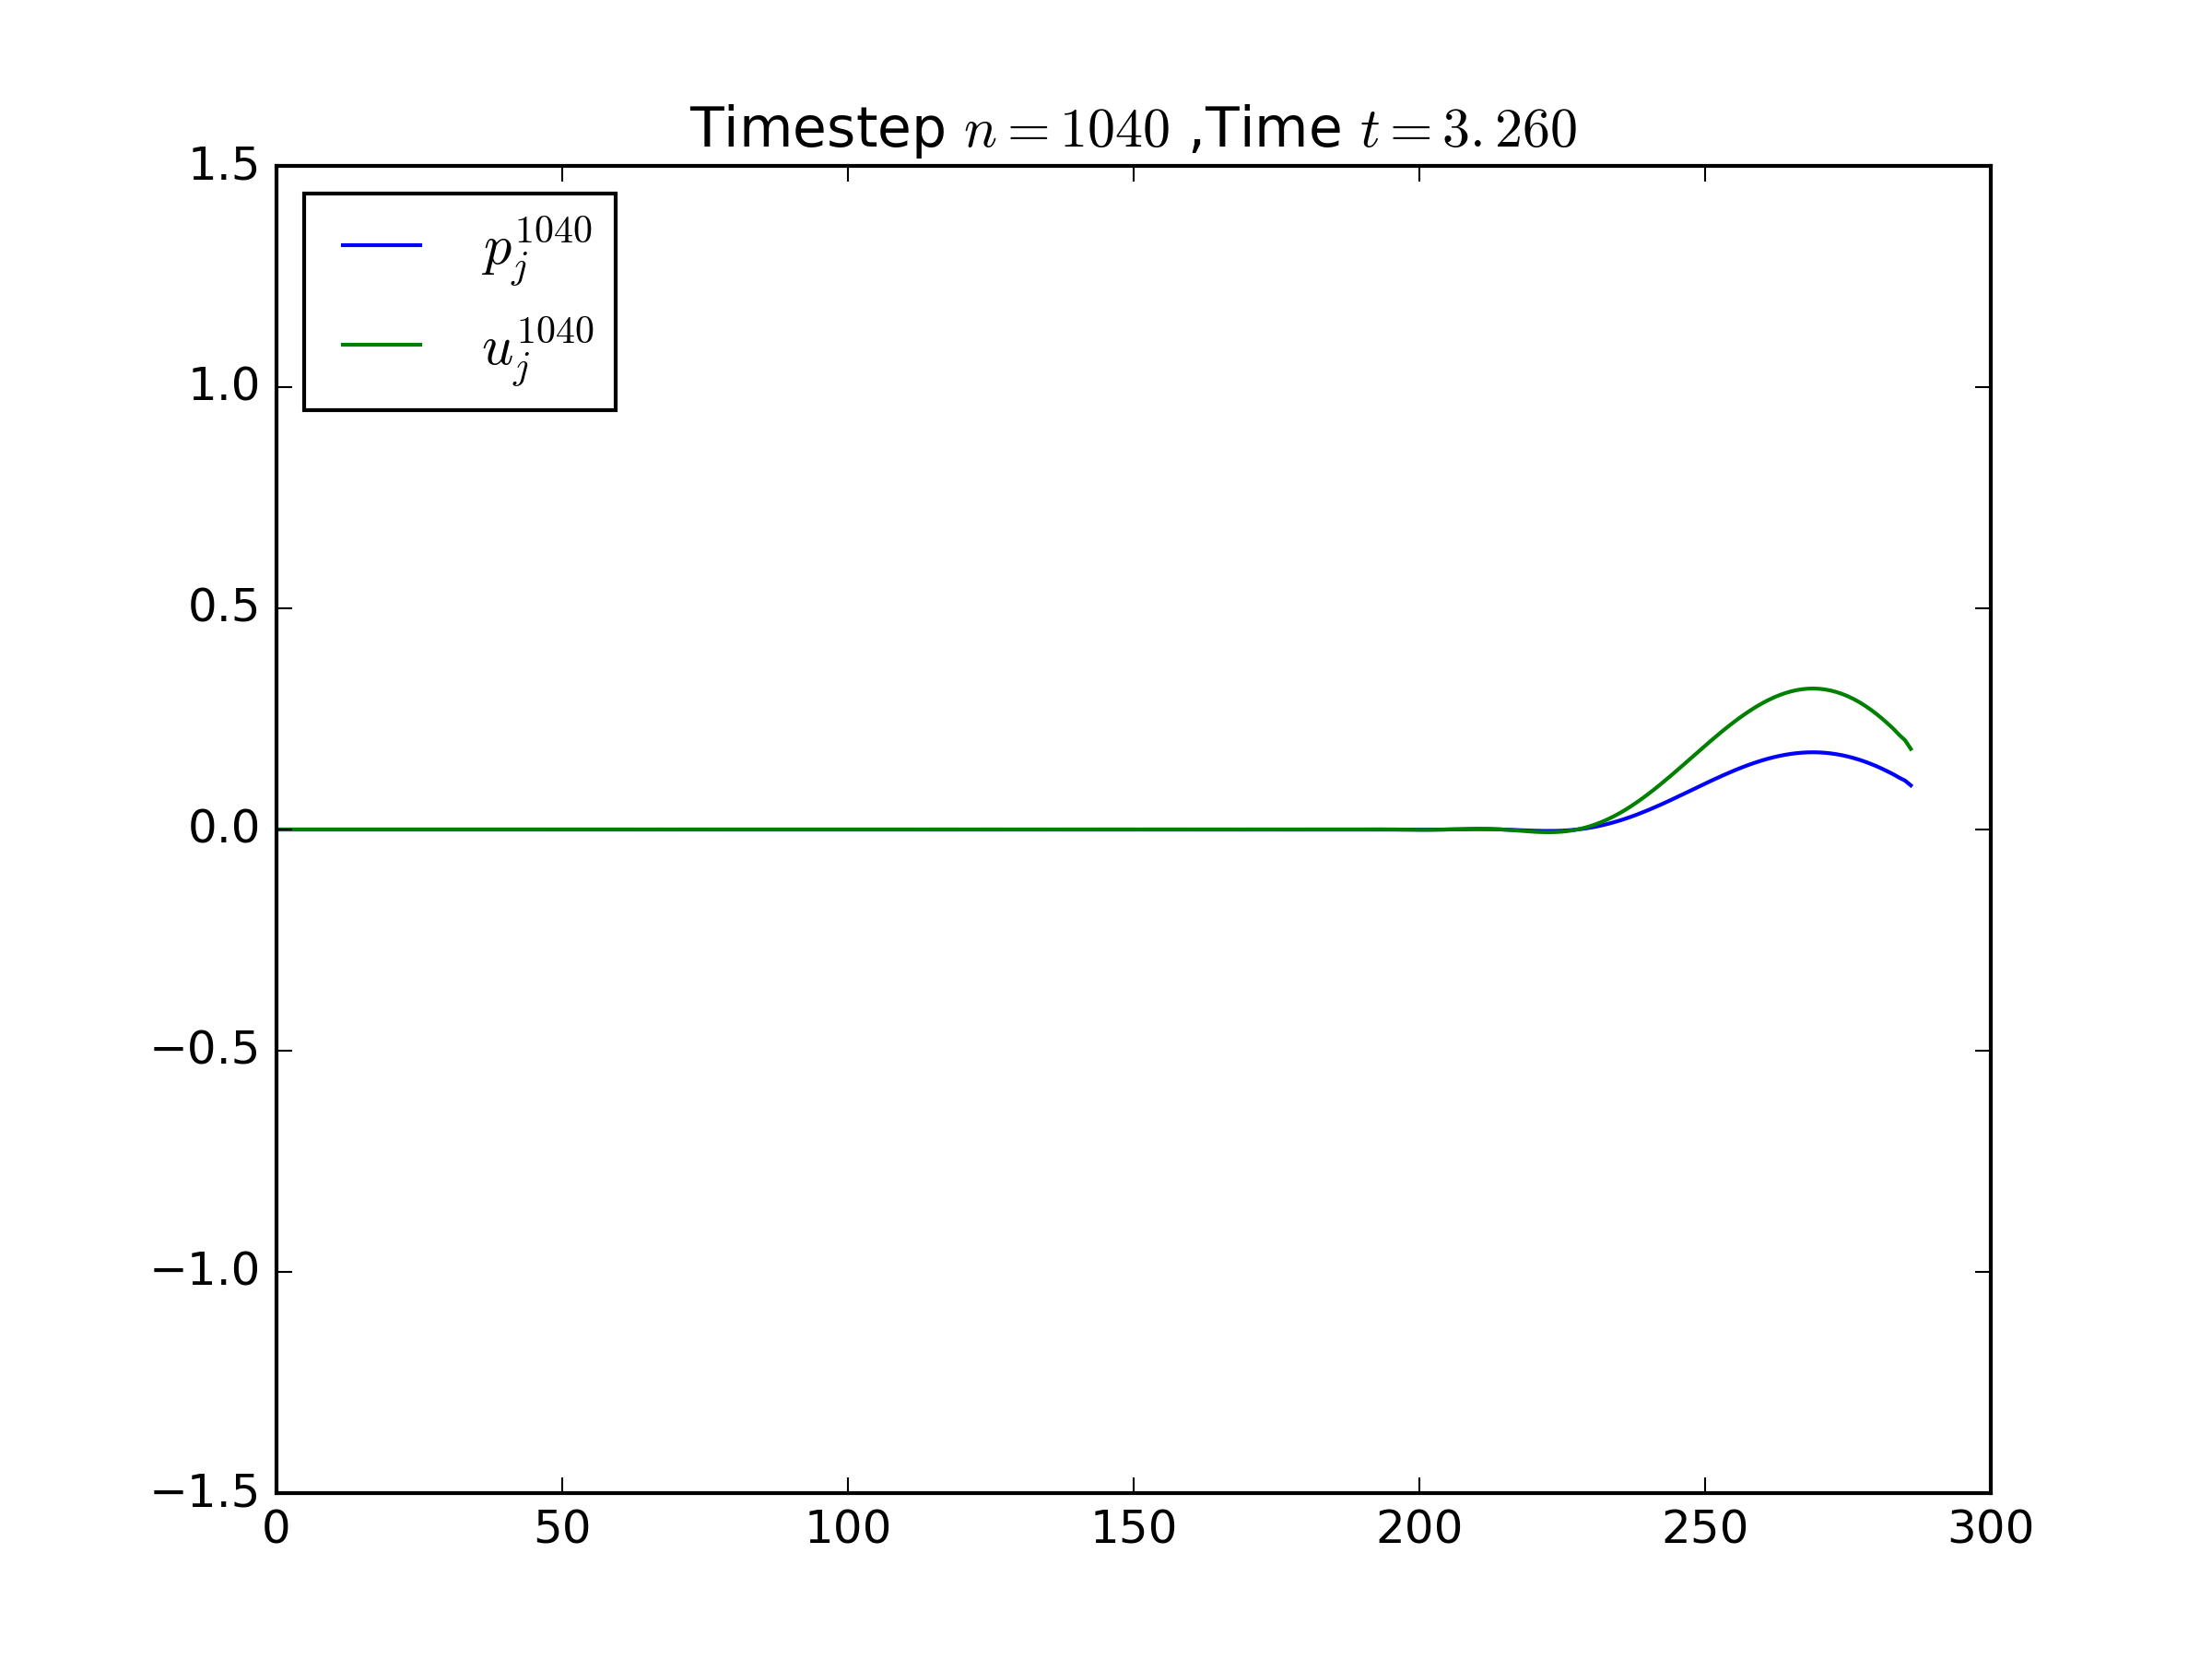
\includegraphics[width=0.31\textwidth]{figures/problem_1_c_104.png}
            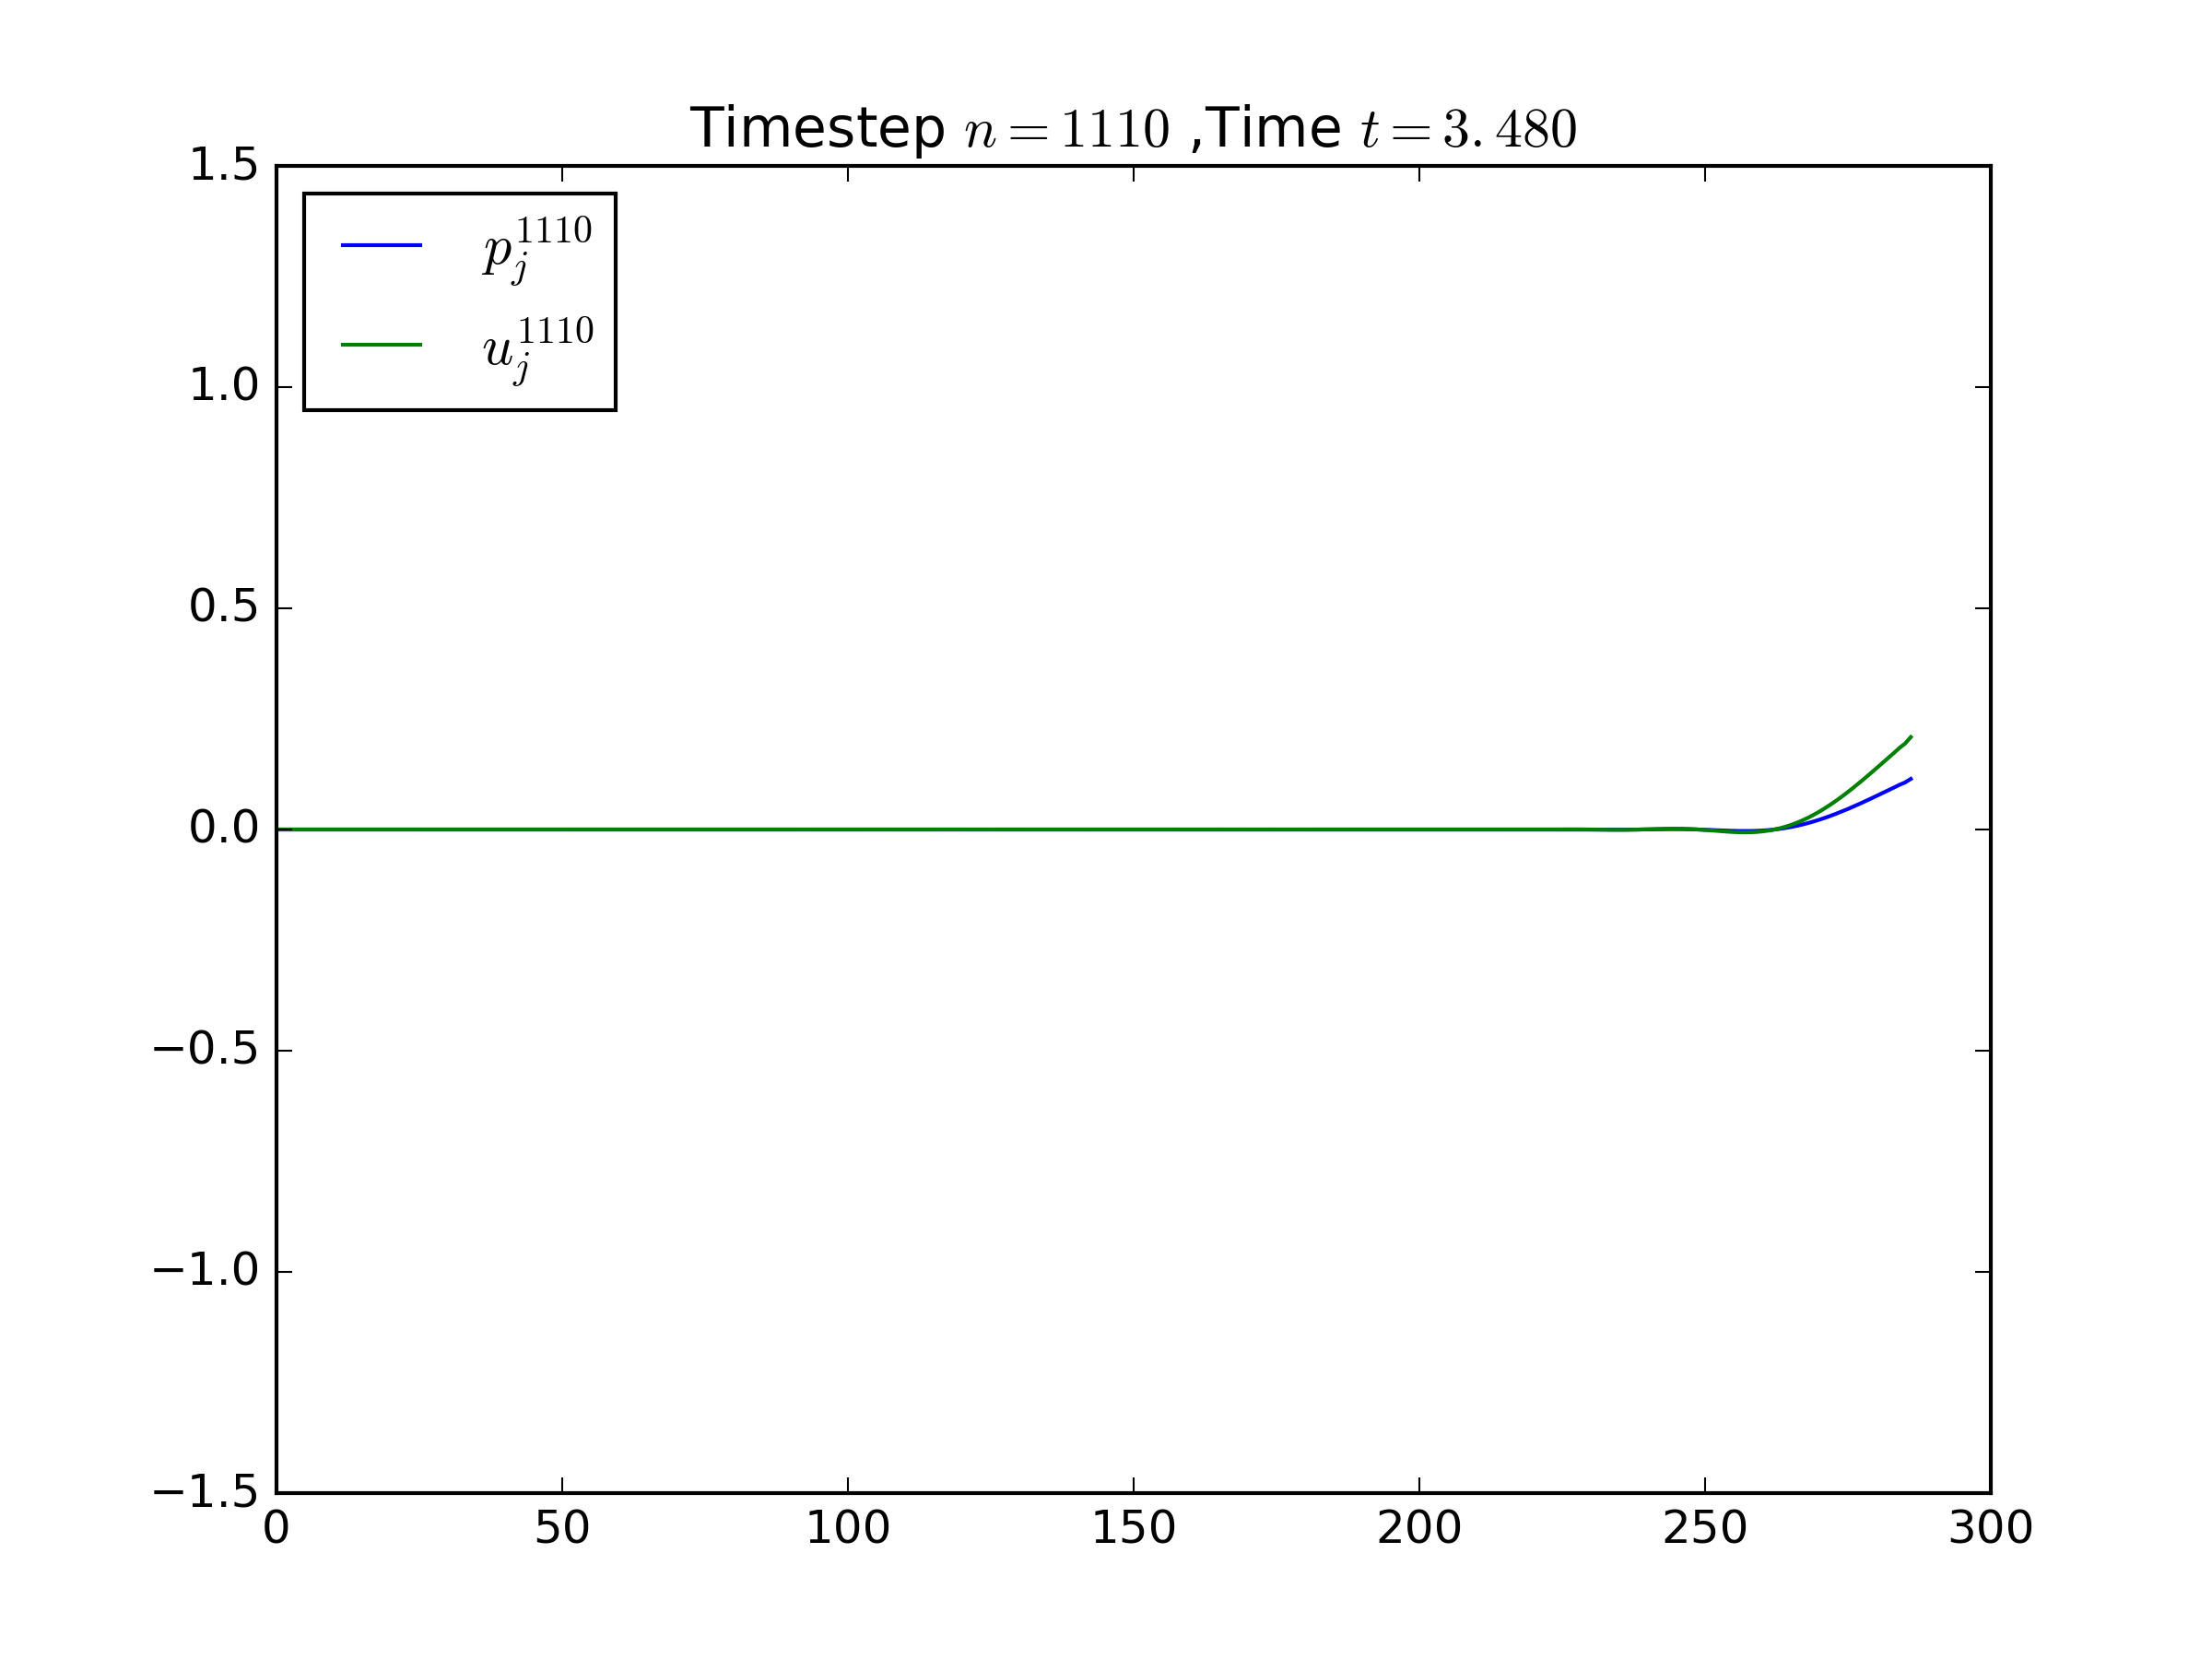
\includegraphics[width=0.31\textwidth]{figures/problem_1_c_111.png}
        \end{figure}
        \FloatBarrier
        \pagebreak

    \item
        Since the matrix $A$ in the system $\vec{u}_t + A\vec{u}_x = \vec{0}$ is diagonalizable, we can write $$\vec{v}_t + \Lambda \vec{v}_x = \vec{0}$$ where
        \begin{align*}
            \Lambda = \qty[\begin{array}{cc}
                \sqrt{K\rho^{-1}} & 0 \\
                0 & -\sqrt{K\rho^{-1}}
            \end{array}], \qquad \vec{v} = V^{-1}\vec{u}, \qquad \text{and }\ \ V = \qty[\begin{array}{cc}
                \sqrt{K\rho} & -\sqrt{K\rho} \\ 1 & 1
            \end{array}].
        \end{align*}
        We can write the ghost cells on the right as
        \begin{align*}
            \vec{u}_{N+1}^n = G_R\vec{u}_N^n
        \end{align*}
        where
        \begin{align*}
            G_R = \frac{1}{2}\qty[\begin{array}{cc}
                1 & \sqrt{K\rho} \\ \frac{1}{\sqrt{K\rho}} & 1
            \end{array}]
        \end{align*}
        Using $\vec{u} = V\vec{v}$, we have $V\vec{v}_{N+1}^n = G_RV\vec{v}_N^n$, or
        \begin{align*}
            \vec{v}_{N+1}^n = V^{-1}G_RV\vec{v}_N^n
        \end{align*}
        However, $V^{-1}G_RV = \qty[\begin{array}{cc}1 & 0 \\ 0 & 0\end{array}]$, so the right side ghost cells in eigenspace are set by
        \begin{align*}
            (v_1)_{N+1}^n &= (v_1)_N^n \\
            (v_2)_{N+1}^n &= 0
        \end{align*}
        Since $v_2$ is the eigenvector with a negative wavespeed, we do not see anything bouncing off the right hand side like we do on the left.  In other words, there is no inward flux of leftward-moving material on the right side.  On the left side, we have
        \begin{align*}
            \vec{u}_{0}^n = G_L\vec{u}_1^n
        \end{align*}
        where
        \begin{align*}
            G_L = \qty[\begin{array}{cc} 1 & 0 \\ 0 & -1 \end{array}].
        \end{align*}
        Using the same transformation, we get
        \begin{align*}
            \vec{v}_0^n = V^{-1}G_LV\vec{v}_1^n
        \end{align*}
        However, $V^{-1}G_LV = \qty[\begin{array}{cc}0 & -1 \\ -1 & 0\end{array}]$, so the left side ghost cells in eigenspace are set by
        \begin{align*}
            (v_1)_0^n &= -(v_2)_1^n \\
            (v_2)_0^n &= -(v_1)_1^n
        \end{align*}
        Since the material ``bounces'' off the left boundary, this description is intuitive since all left-moving material becomes right-moving material, and all right-moving material becomes left-moving material.
        
\end{enumerate}







\problem{Problem 2}{Write a program to solve the linear advection equation, $$u_t + au_x = 0,$$ on the unit interval using a finite volume method of the form $$u_j^{n+1} = u_j^n - \frac{\Dt}{\Dx}\qty(F_{j+\nicefrac{1}{2}} - F_{j-\nicefrac{1}{2}}).$$  Use the numerical flux function $$F_{j-\nicefrac{1}{2}} = F_{j-\nicefrac{1}{2}}^\text{up} + \frac{\abs{a}}{2}\qty(1 - \abs{\frac{a\Dt}{\Dx}})\delta_{j-\nicefrac{1}{2}},$$ where $F_{j - \nicefrac{1}{2}}^\text{up}$ is the upwinding flux,
\begin{align*}
    F_{j-\nicefrac{1}{2}}^\text{up} = \begin{cases}
        au_{j-1} & \text{ if } a > 0 \\
        au_j & \text{ if } a < 0,
    \end{cases}
\end{align*}
and $\delta_{j-\nicefrac{1}{2}}$ is the limited difference.  Let $\Delta u_{j-\nicefrac{1}{2}} = u_j - u_{j-1}$ denote the jump in $u$ across the edge at $x_{j-\nicefrac{1}{2}}$.  The limited difference is $$\delta_{j-\nicefrac{1}{2}} = \phi(\theta_{j-\nicefrac{1}{2}})\Delta u_{j-\nicefrac{1}{2}},$$ where $$\theta_{j-\nicefrac{1}{2}} = \frac{\Delta u_{J_\text{up}-\nicefrac{1}{2}}}{\Delta u_{j - \nicefrac{1}{2}}},$$ and
\begin{align*}
    J_\text{up} = \begin{cases}
        j - 1 & \text{ if } a > 0 \\
        j + 1 & \text{ if } a < 0
    \end{cases}.
\end{align*}
Note that you will need two ghost cells on each end of the domain.  Write your program so that you may choose from the different limiter functions listed below.

\begin{tabular}{ll}
    (1) Upwinding & $\phi(\theta) = 0$ \\
    (2) Lax-Wendroff & $\phi(\theta) = 1$ \\
    (3) Beam-Warming & $\phi(\theta) = \theta$ \\
    (4) minmod & $\phi(\theta) = \text{minmod}(1,\theta)$ \\
    (5) superbee & $\phi(\theta) = \max(0,\min(1,2\theta),\min(2,\theta))$ \\
    (6) MC & $\phi(\theta) = \max(0,\min(\frac{1+\theta}{2},2,2\theta))$ \\
    (7) van Leer & $\phi(\theta) = \dfrac{\theta + \abs{\theta}}{1 + \abs{\theta}}$
\end{tabular}

The first three are linear methods that we have already studied, and the last four are high-resolution methods.

Solve the advection equation with $a = 1$ with periodic boundary conditions for the different initial conditions listed below until time $t = 5$ at Courant number $0.9$.

\begin{tabular}{ll}
    (a) Wave packet: & $u(x,0) = \cos(16\pi x)\exp(-50(x-0.5)^2)$ \\
    (b) Smooth, low frequency: & $u(x,0) = \sin(2\pi x)\sin(4\pi x)$ \\
    (c) Step function: & $u(x,0) = u(x,0) = \begin{cases}1 & \text{if } \abs{x - \nicefrac{1}{2}}<\frac{1}{4} \\ 0 & \text{ otherwise} \end{cases}$
\end{tabular}

Compare the results with the exact solution, and comment on the solutions generated by the different methods.  How do the different high-resolution methods perform in the different tests?  What high-resolution method would you chose to use in practice?
}

First I defined the limiter function using a user-defined choice of $\phi$.
\lstinputlisting[language=Python,firstline=84,lastline=108]{operators.py}
Then I defined the index $J_\text{up}$ based on the index $j$ and flow direction $a$
\lstinputlisting[language=Python,firstline=77,lastline=82]{operators.py}
I defined a $\Delta$ function, given $u$ and $j$:
\lstinputlisting[language=Python,firstline=65,lastline=67]{operators.py}
and used that to define $\theta_{j-\nicefrac{1}{2}}$
\lstinputlisting[language=Python,firstline=69,lastline=75]{operators.py}
Next I defined the limited differences $\delta_{j-\nicefrac{1}{2}}$
\lstinputlisting[language=Python,firstline=53,lastline=63]{operators.py}
Then I defined the upwinding flux $F_{j-\nicefrac{1}{2}}^\text{up}$
\lstinputlisting[language=Python,firstline=36,lastline=41]{operators.py}
and finally the numerical flux function $F_{j-\nicefrac{1}{2}}$
\lstinputlisting[language=Python,firstline=43,lastline=51]{operators.py}
The numerical flux function is used to define the recursion.  I made a function \verb|make_FV_method| to construct a recursive step.
\lstinputlisting[language=Python,firstline=8,lastline=34]{operators.py}
To actually use the code, I defined an initial condition function
\lstinputlisting[language=Python,firstline=1,lastline=12]{code_for_homework.py}
then rolled it all together with the following code:
\lstinputlisting[language=Python,firstline=14,lastline=43]{code_for_homework.py}

\begin{enumerate}[\ \ (a)]
    \pagebreak
    \item
        Here are the results for all seven methods for $u_0(x) = \cos(16\pi x)\exp(-50\qty(x - 0.5)^2)$.
        \begin{figure}[ht!]
            \centering
            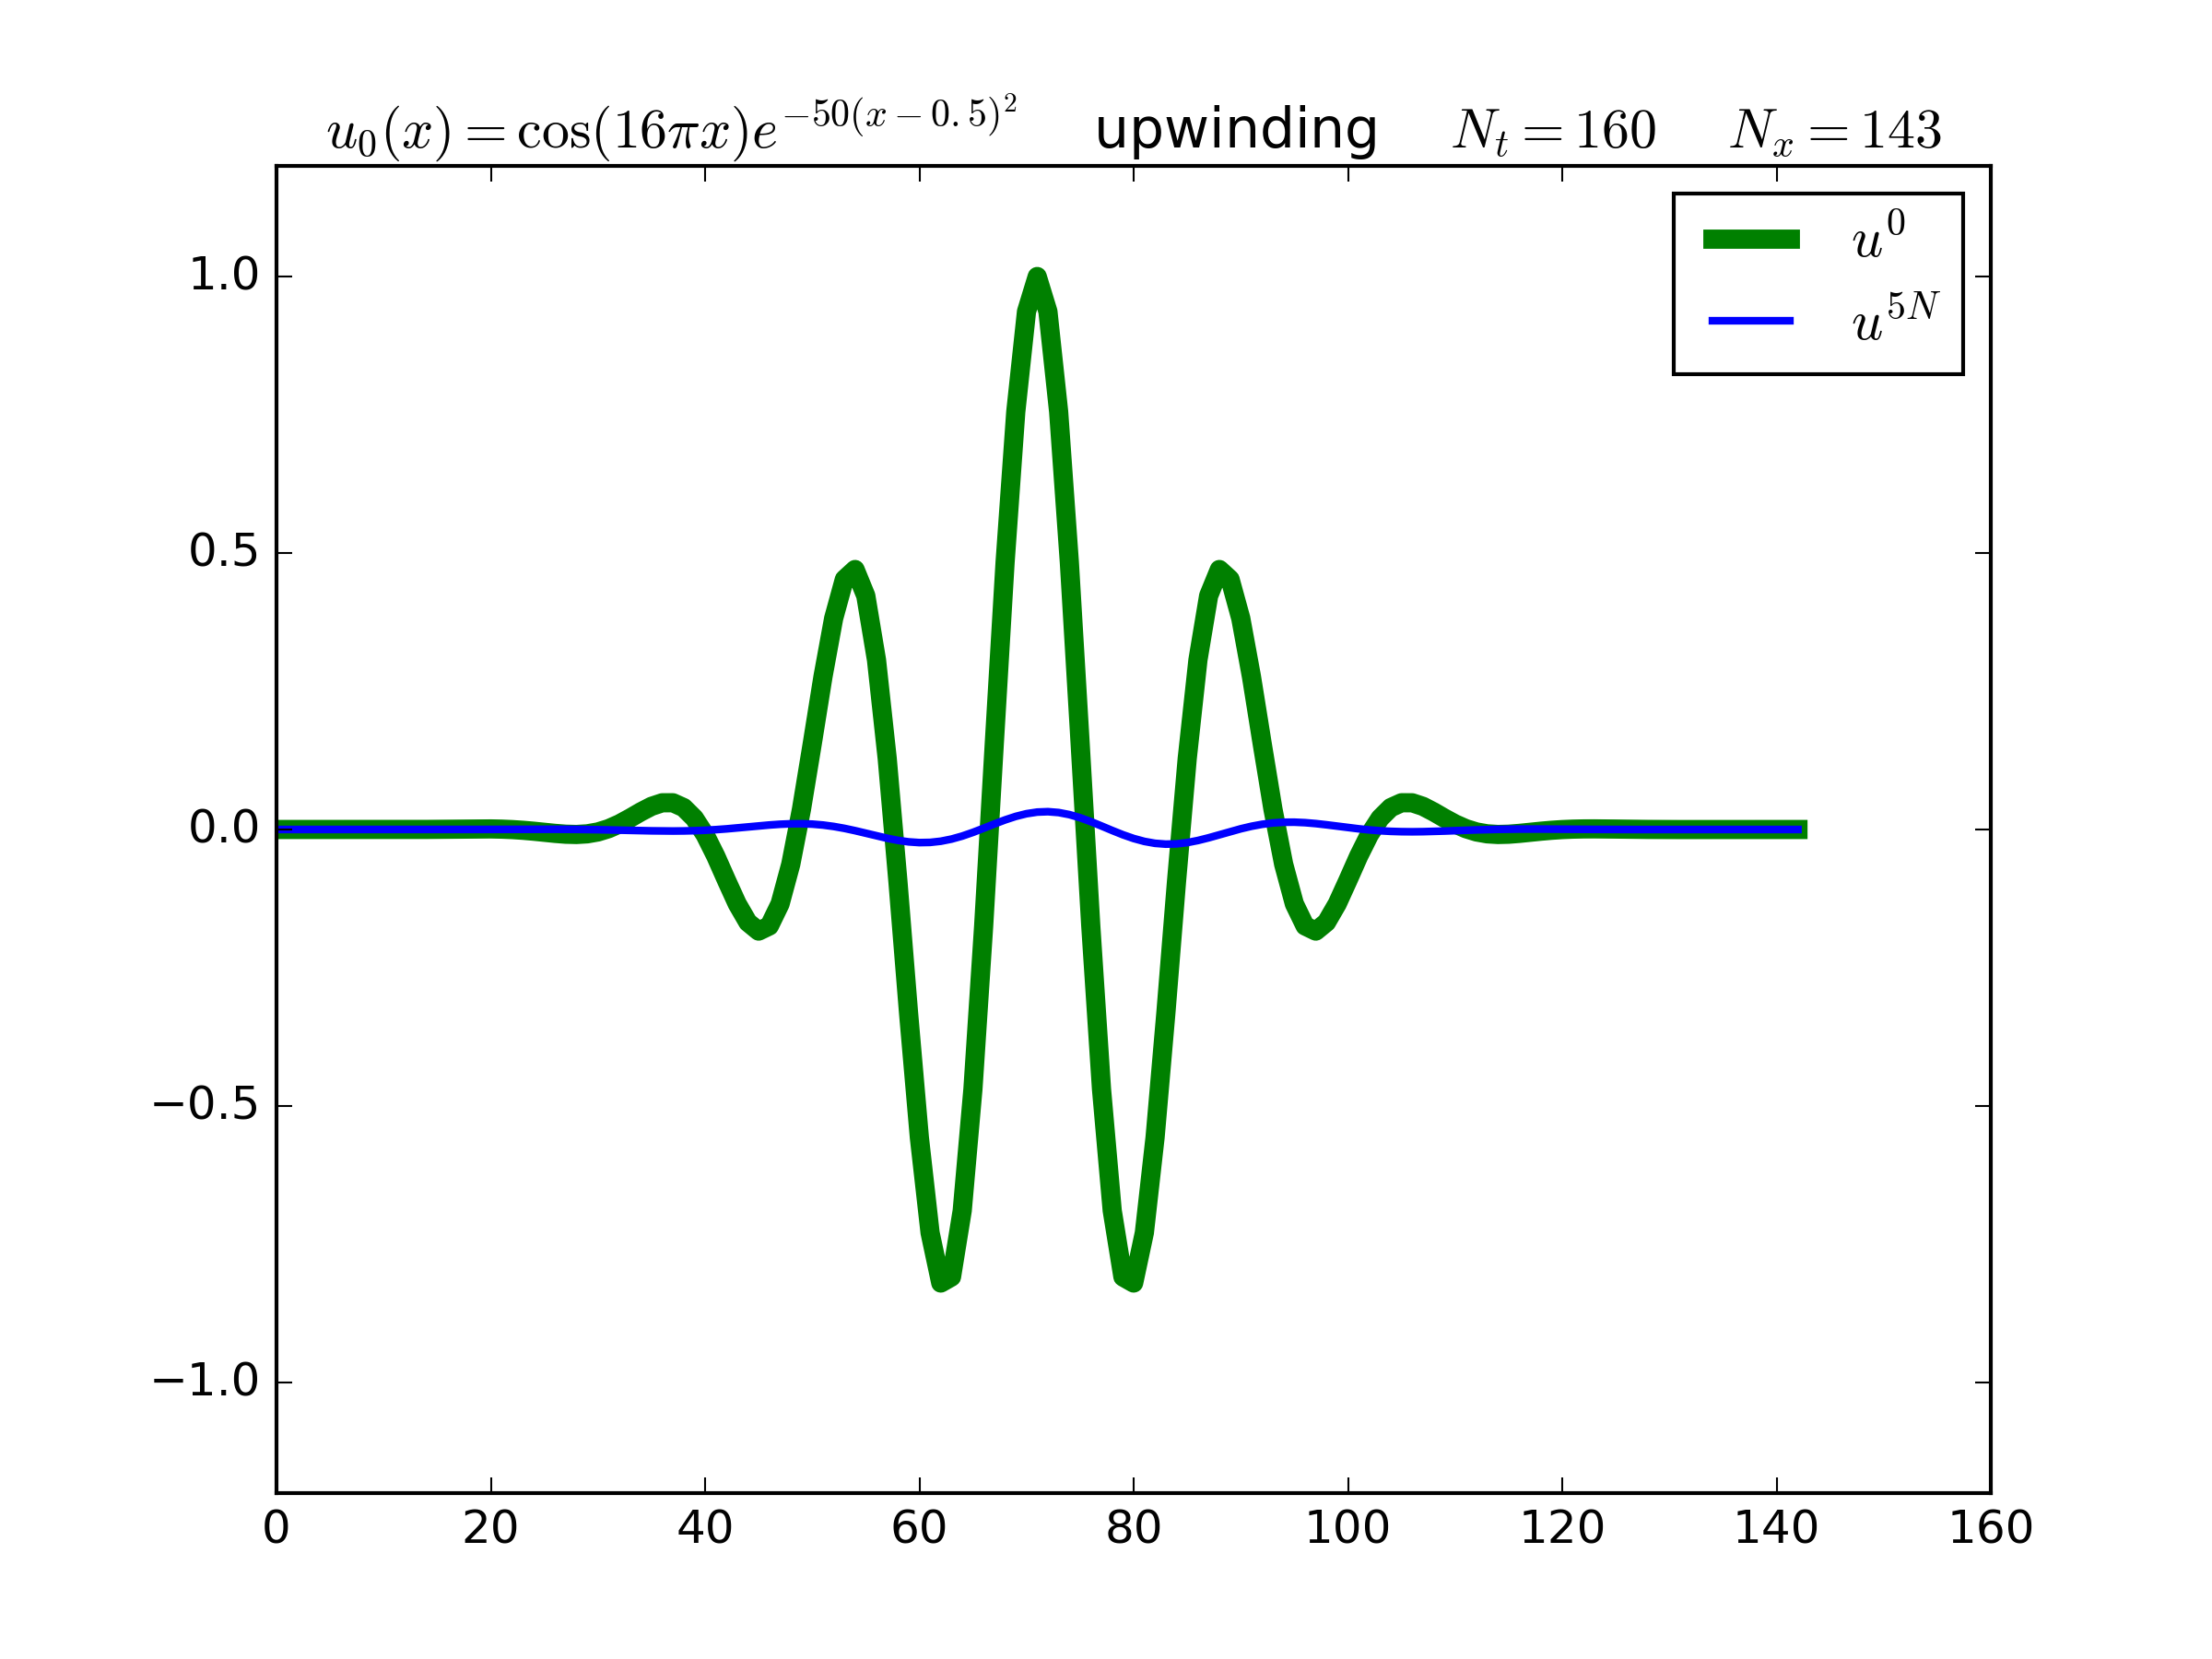
\includegraphics[width=0.29\textwidth]{figures/power_4/problem_2_1_1_a.png}
            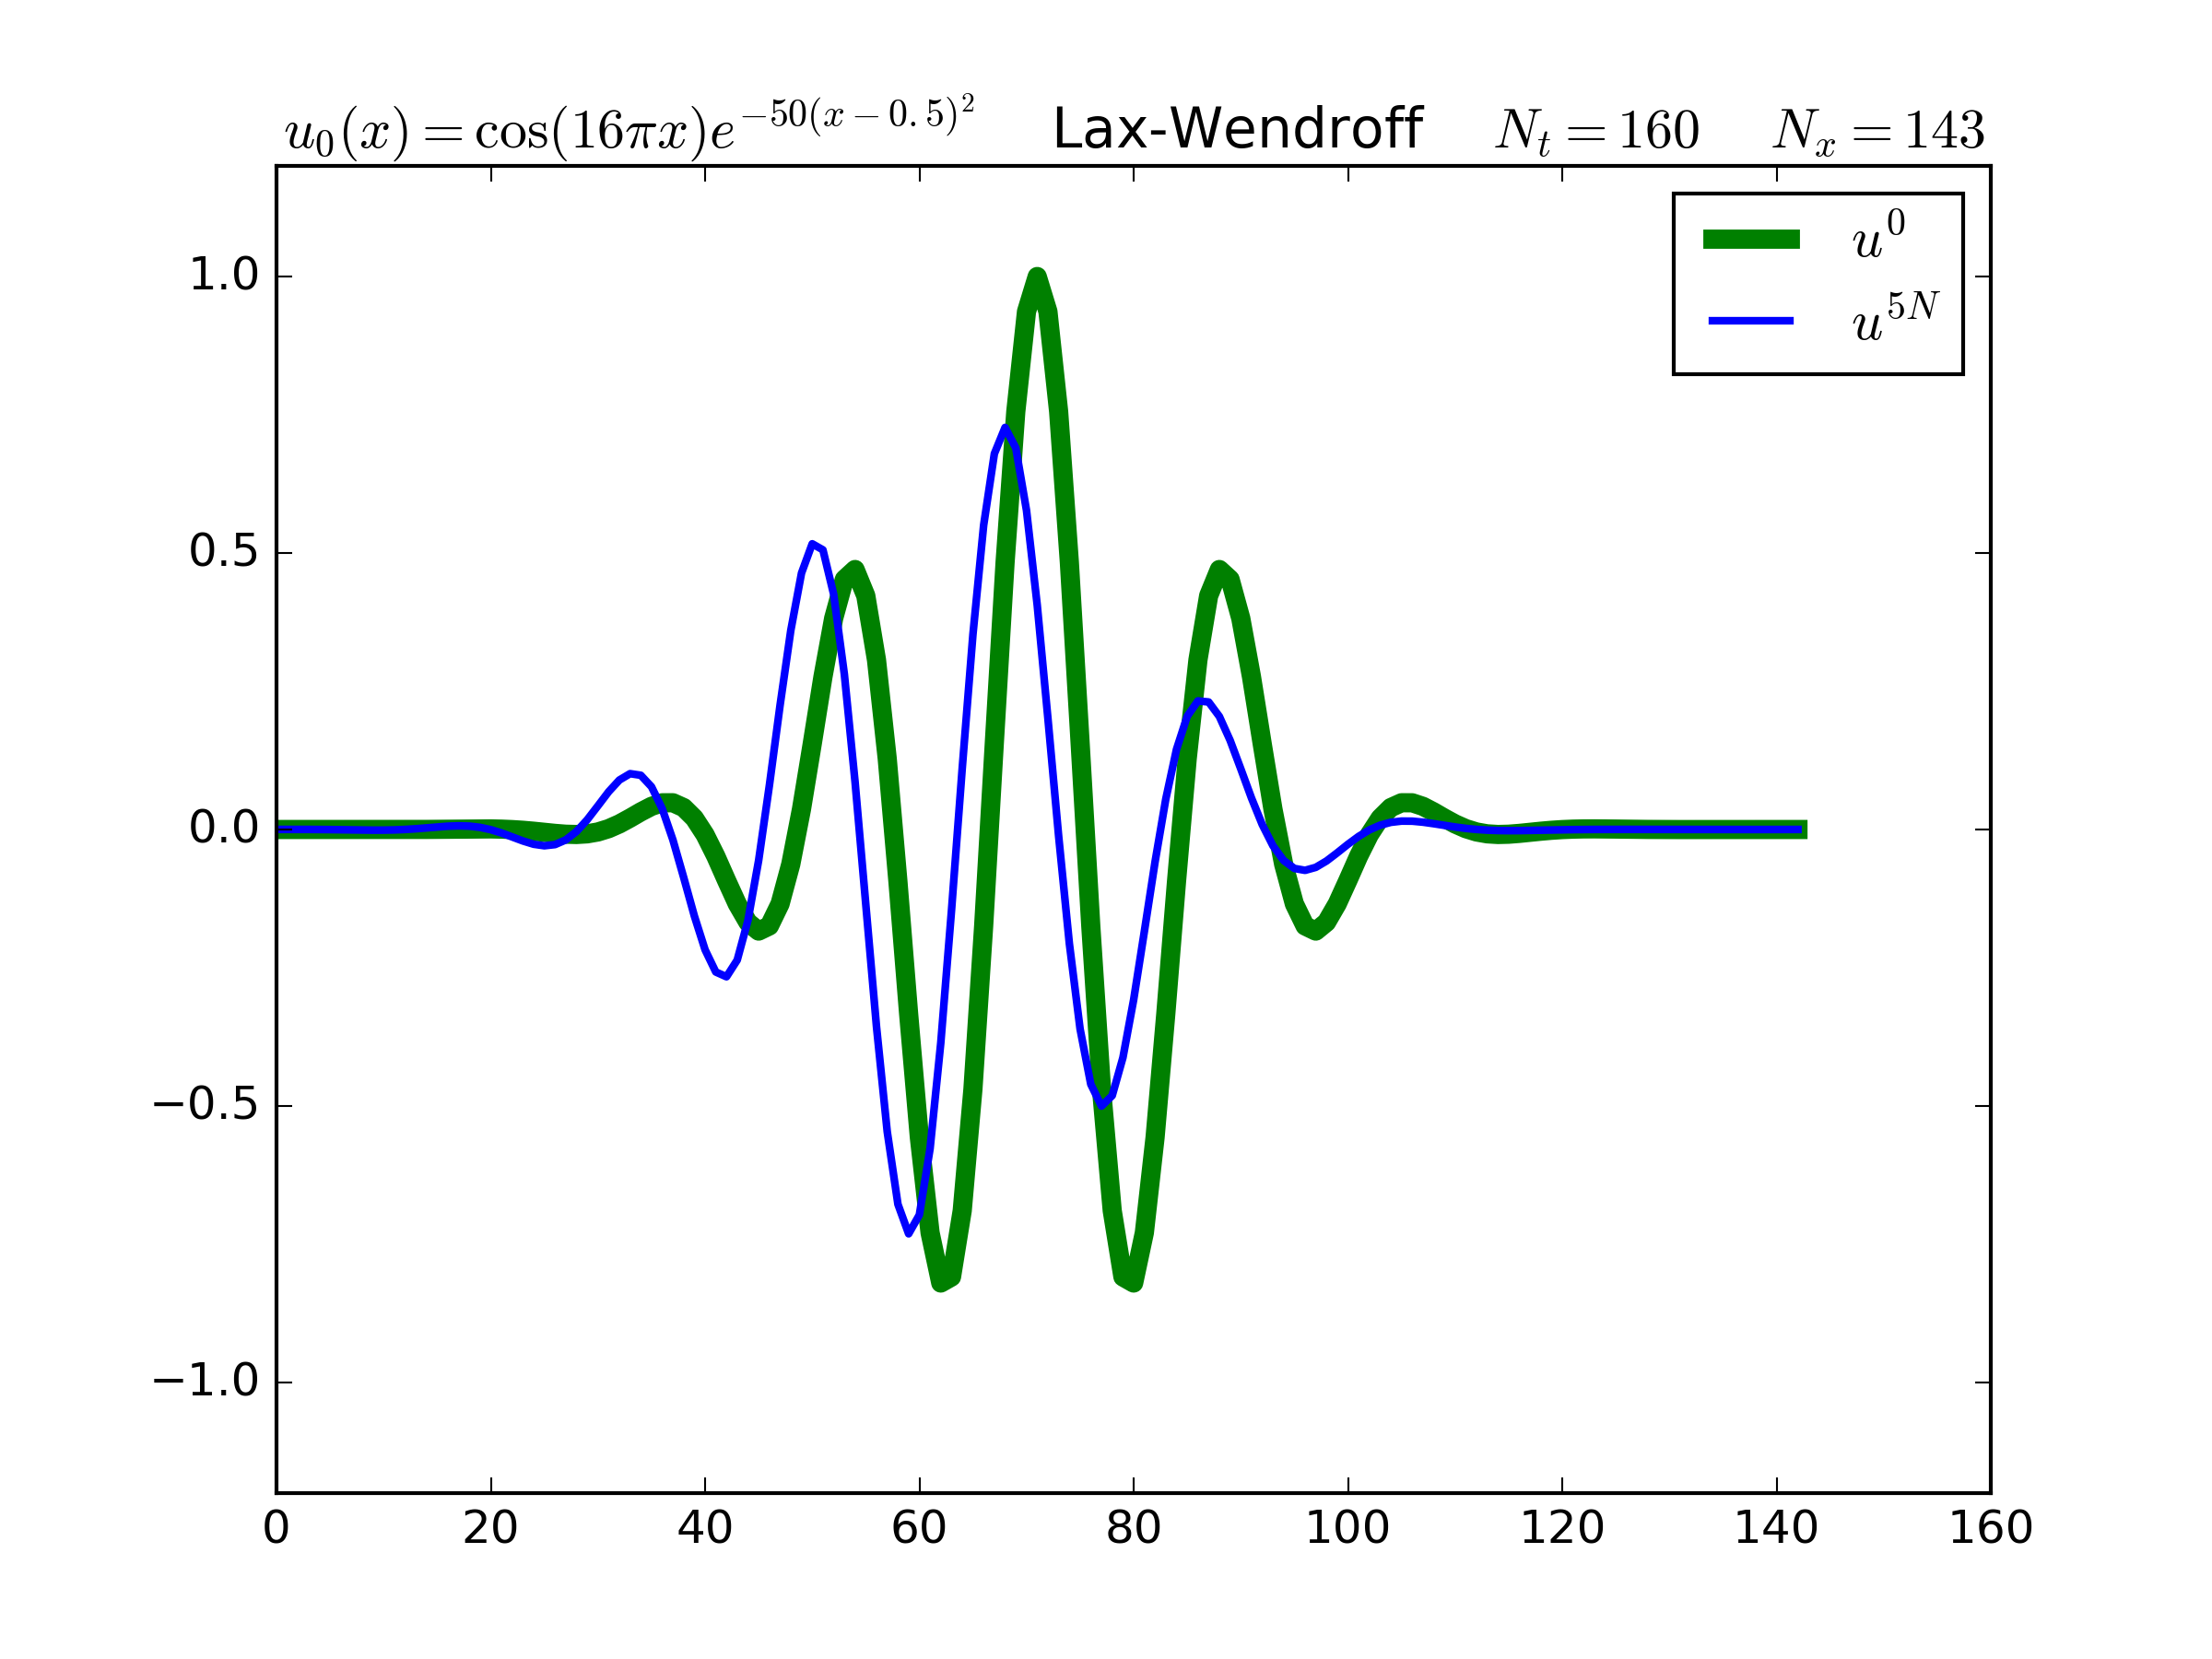
\includegraphics[width=0.29\textwidth]{figures/power_4/problem_2_1_2_a.png}
            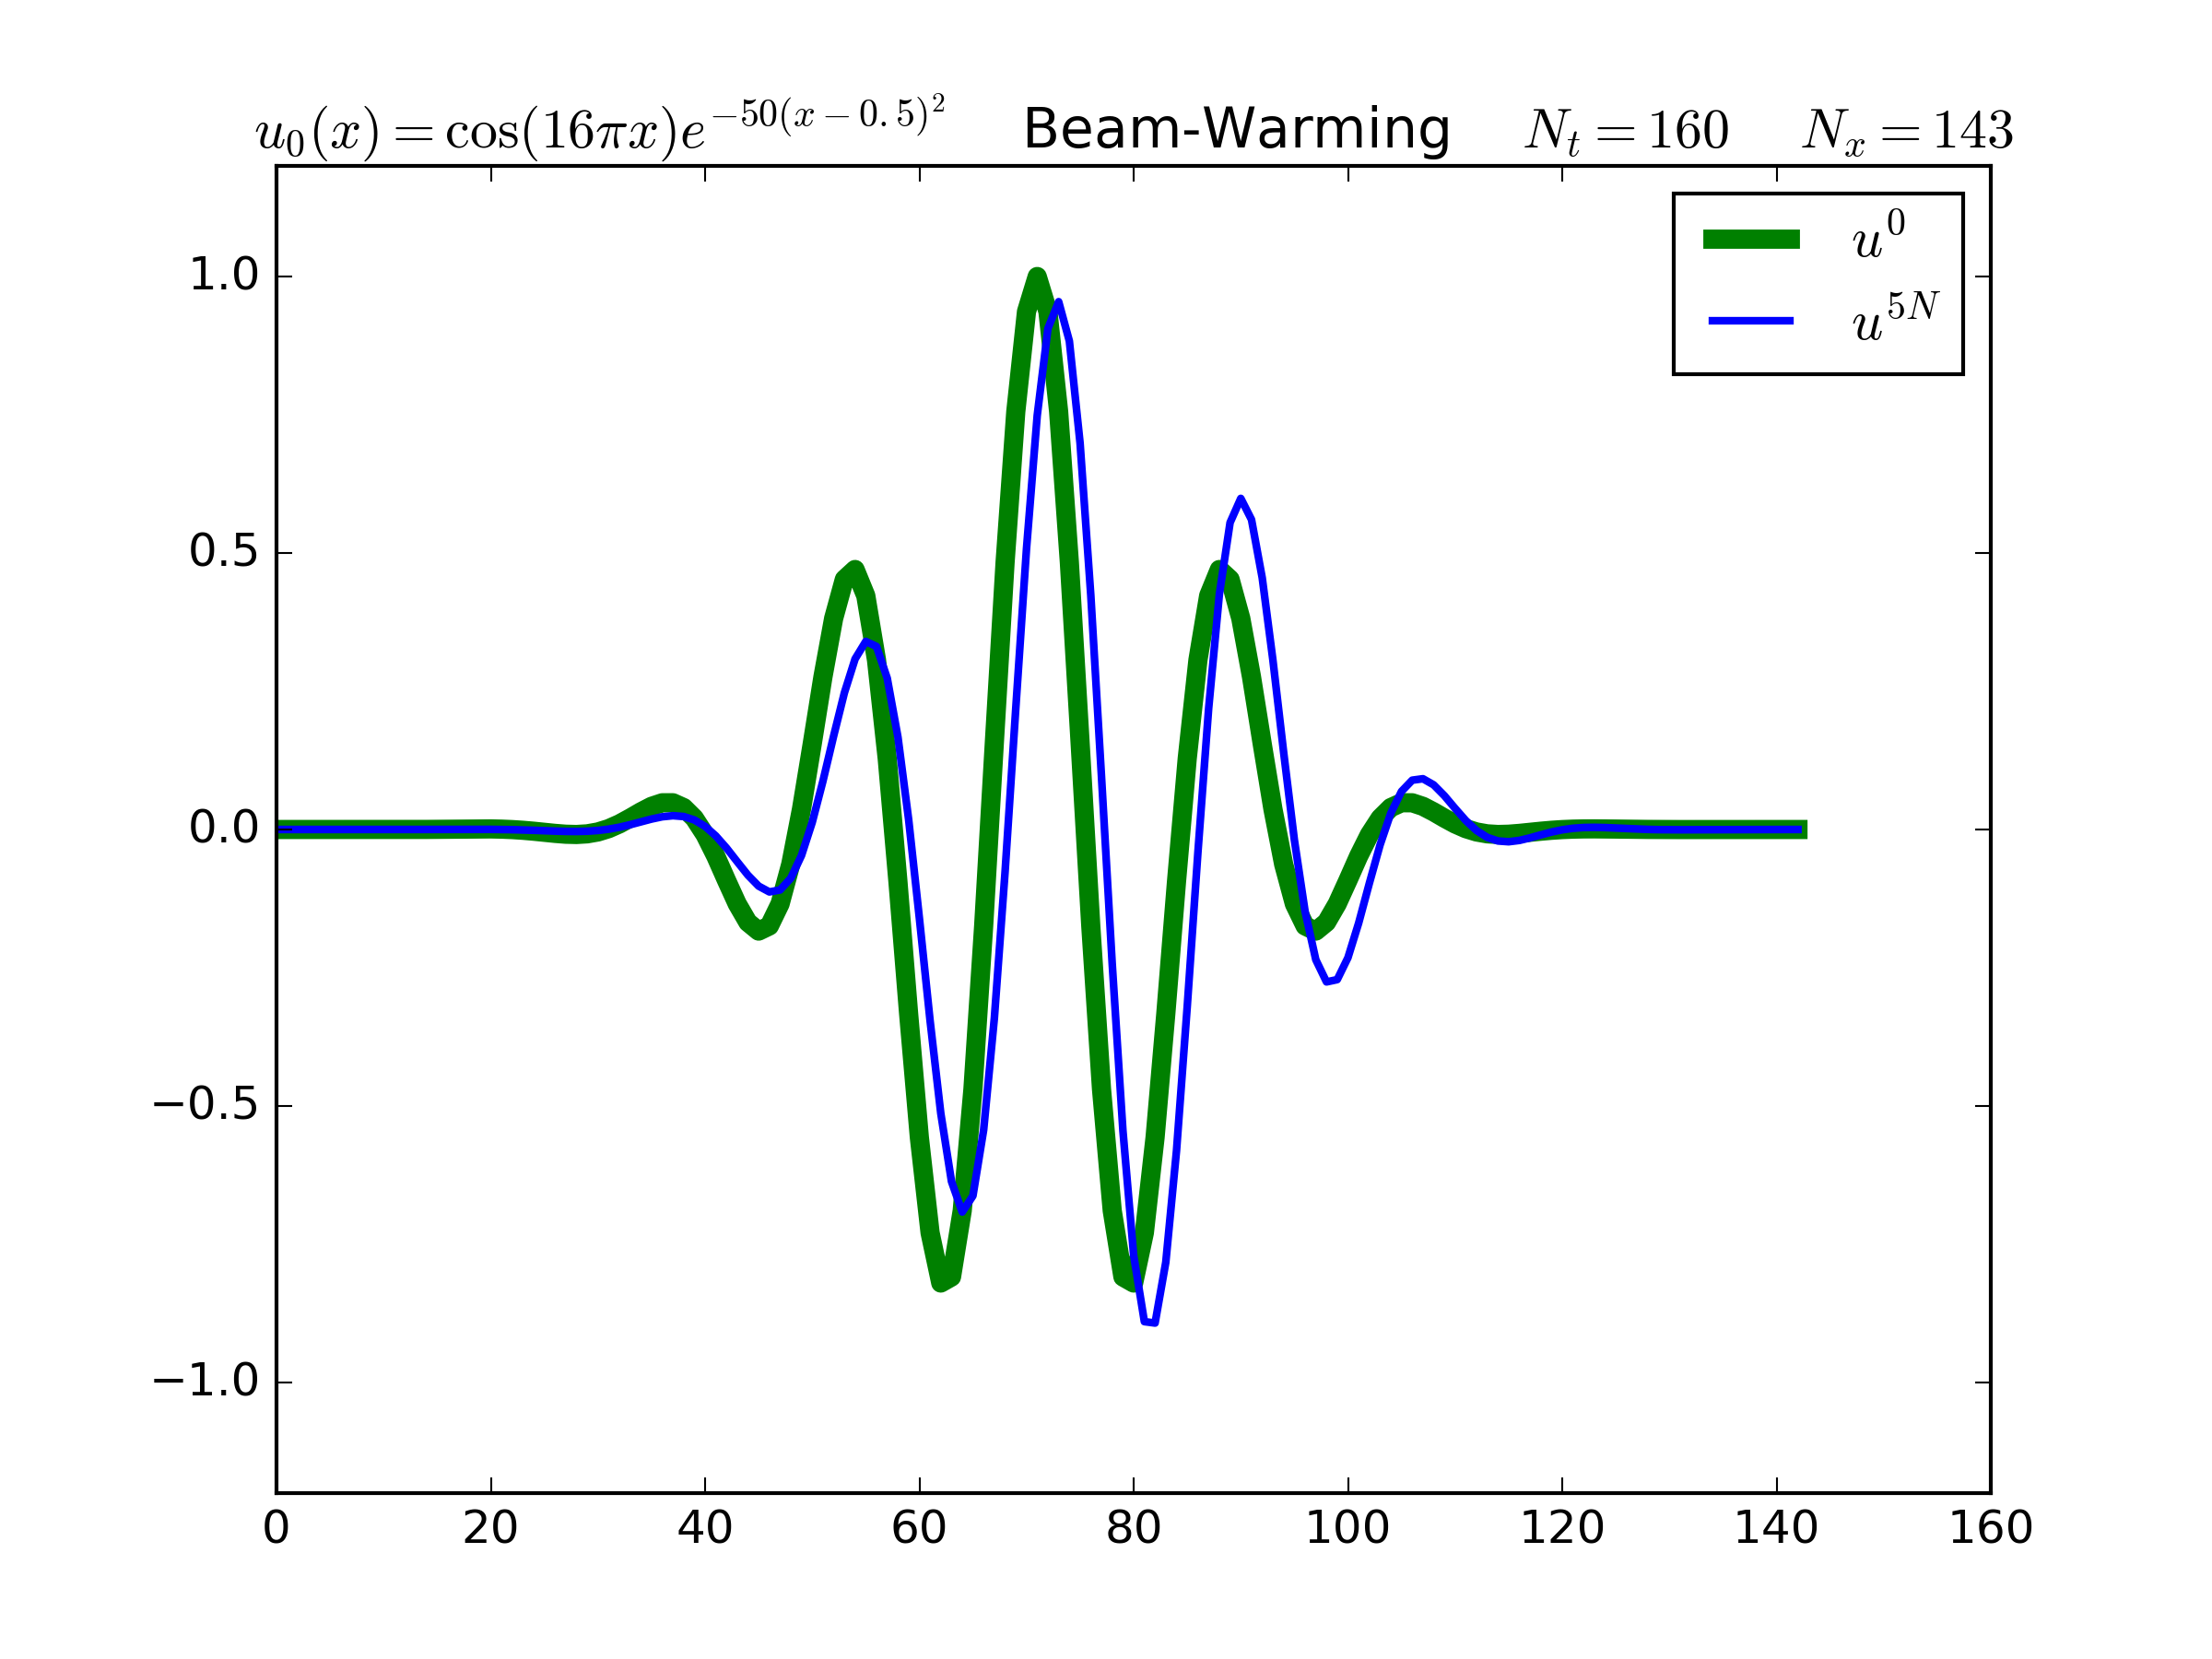
\includegraphics[width=0.29\textwidth]{figures/power_4/problem_2_1_3_a.png}
            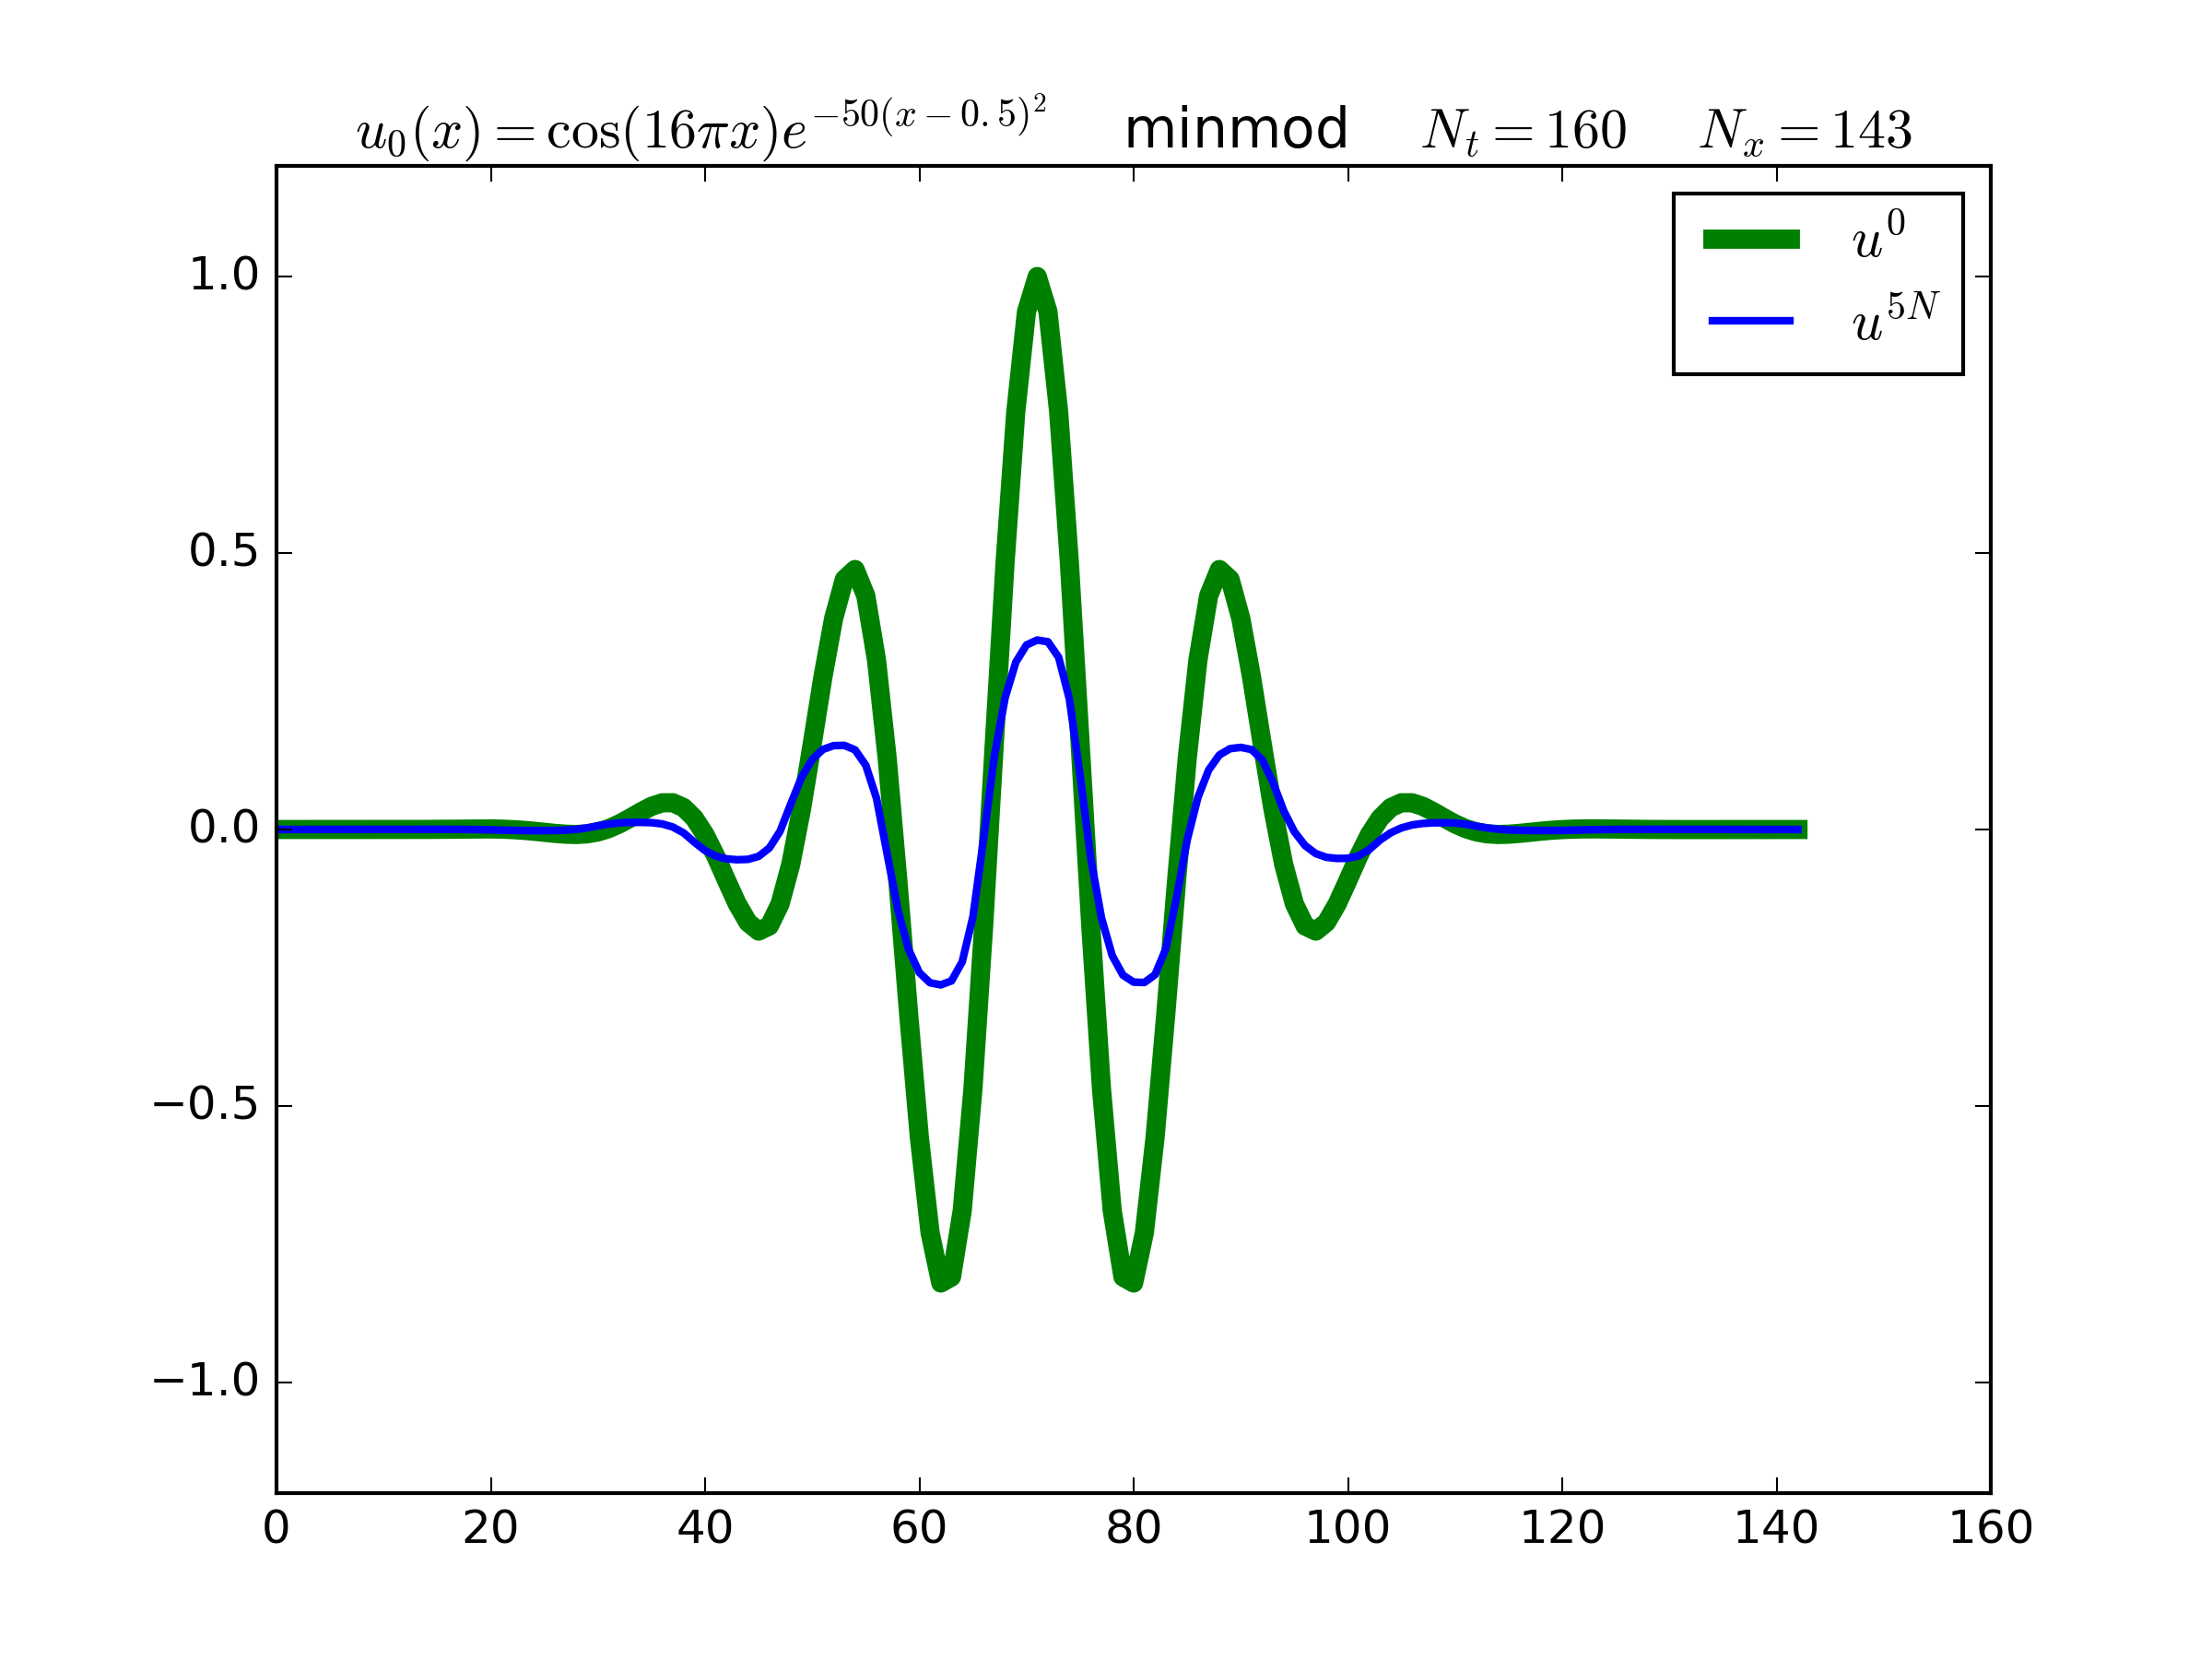
\includegraphics[width=0.29\textwidth]{figures/power_4/problem_2_1_4_a.png}
            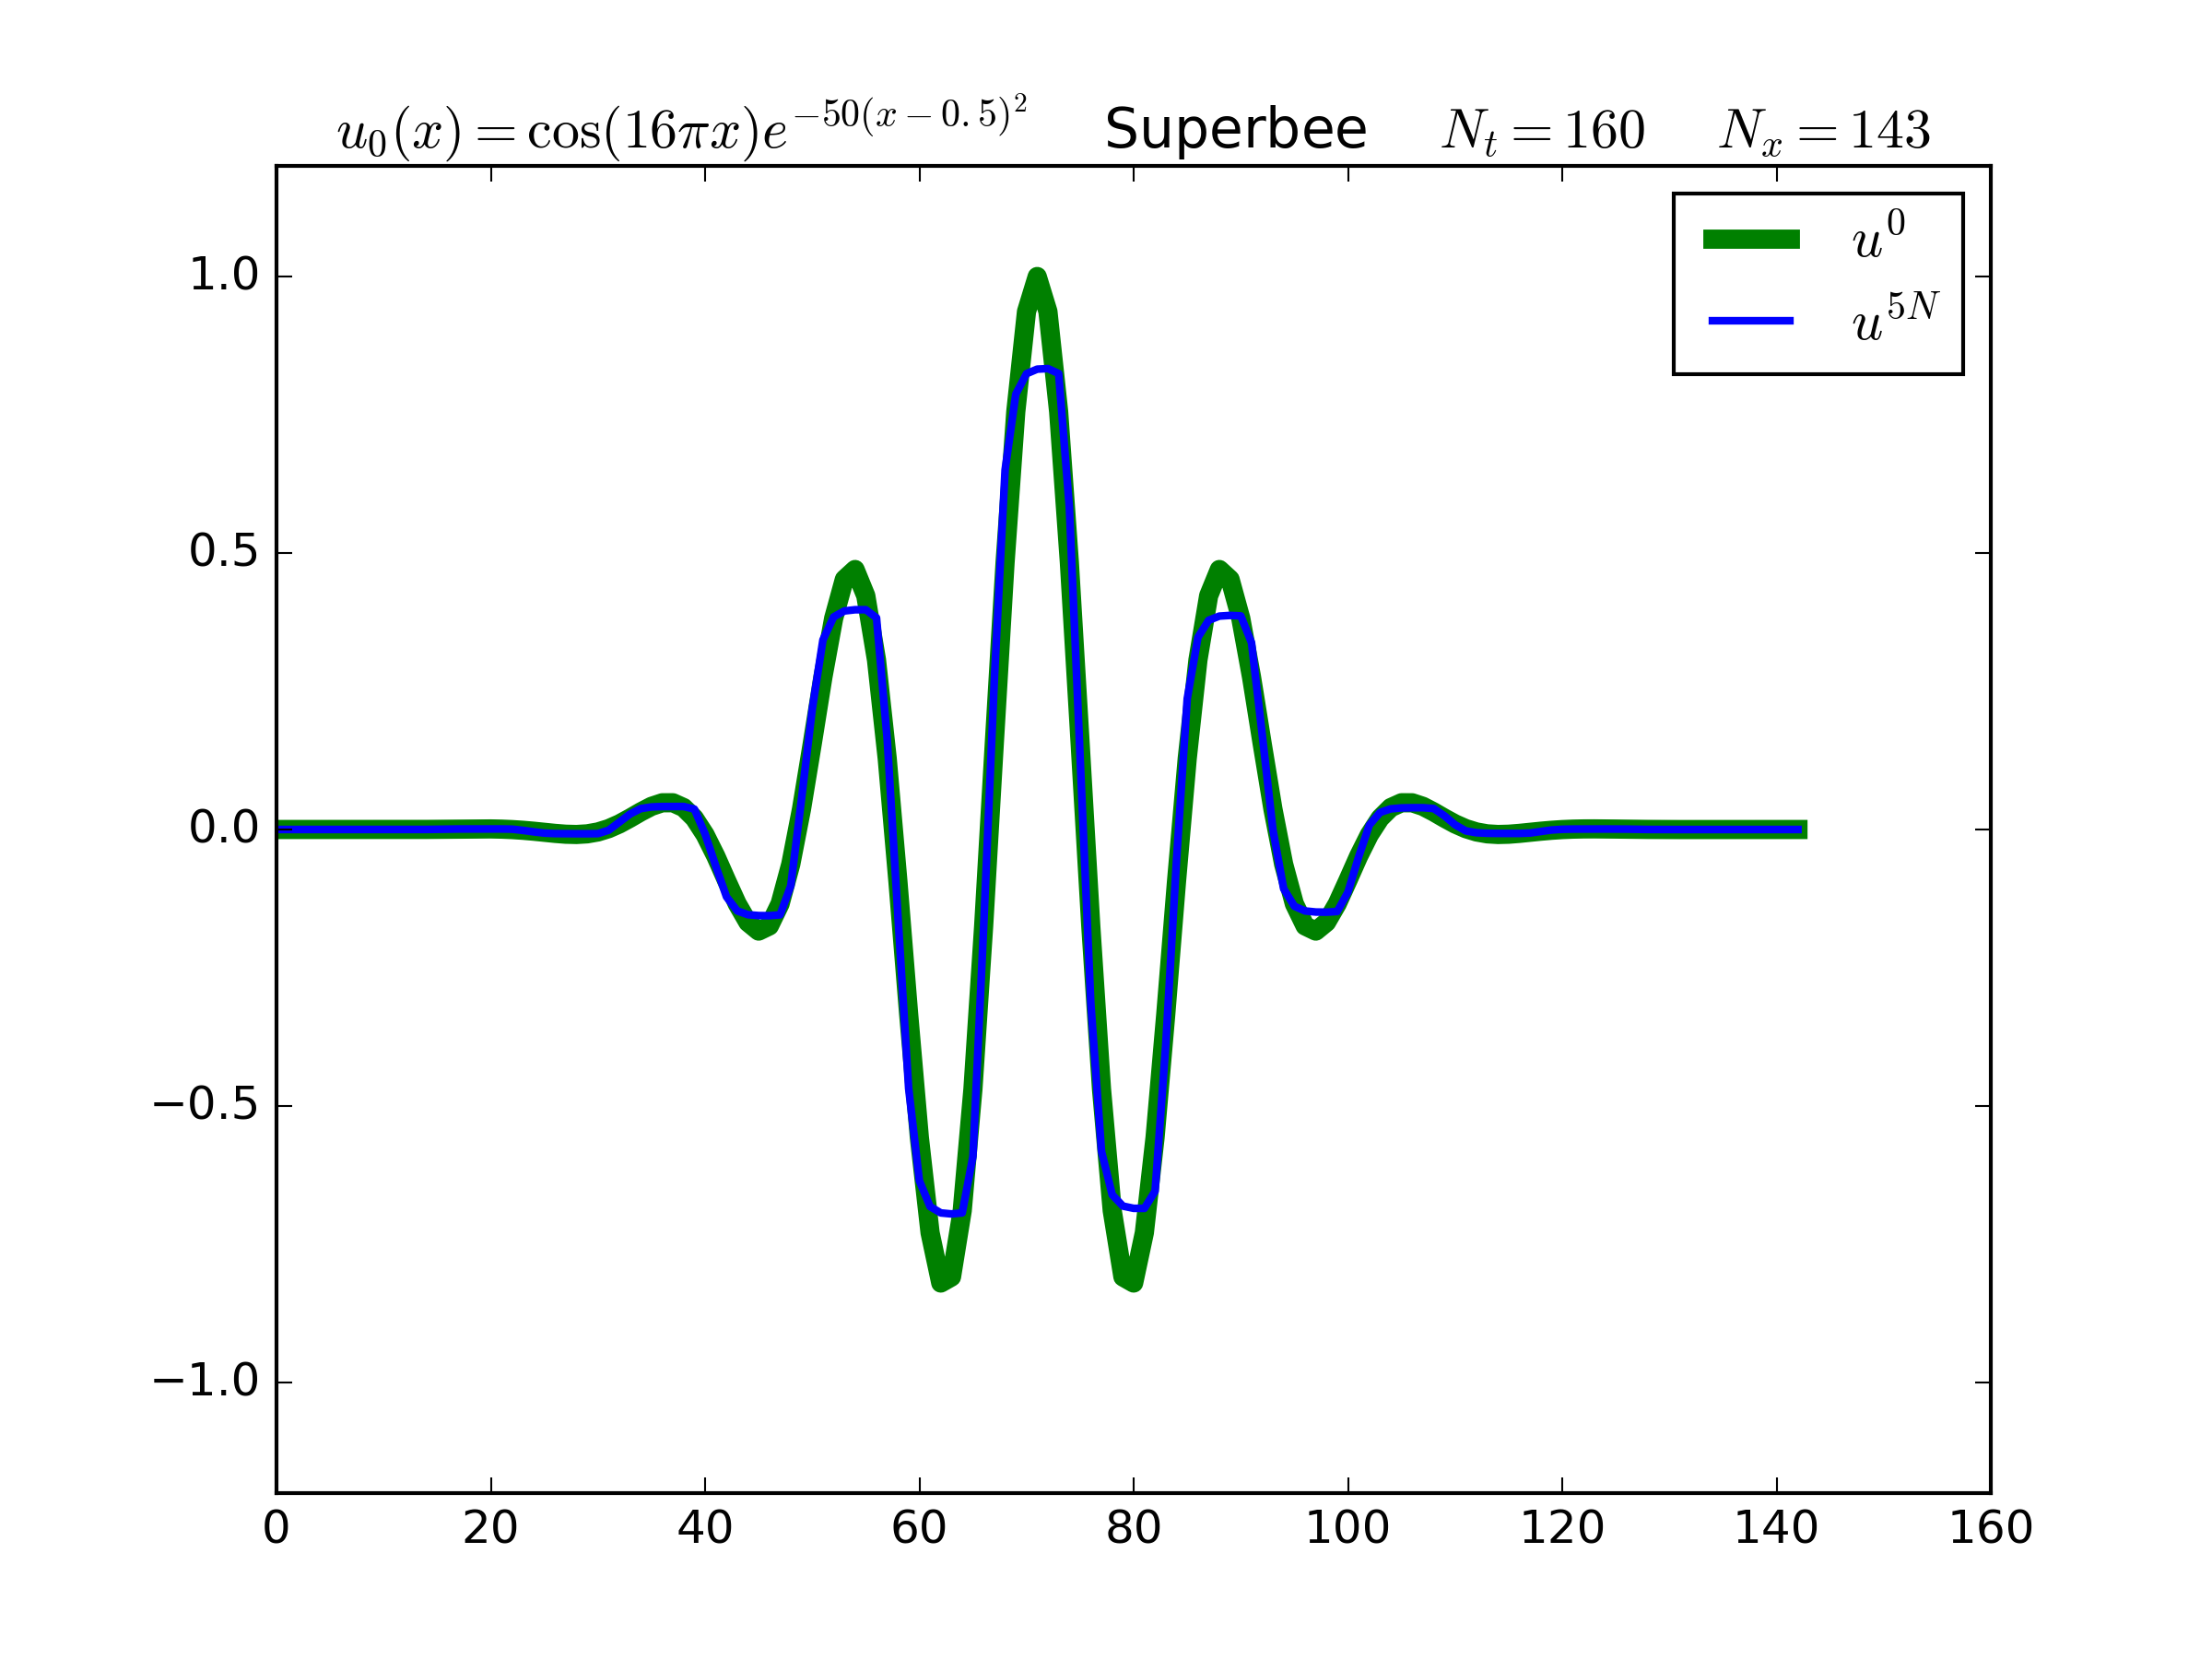
\includegraphics[width=0.29\textwidth]{figures/power_4/problem_2_1_5_a.png}
            \includegraphics[width=0.29\textwidth]{figures/power_4/problem_2_1_6_a.png}
            \includegraphics[width=0.29\textwidth]{figures/power_4/problem_2_1_7_a.png}\\
            \includegraphics[width=0.29\textwidth]{figures/power_4/problem_2_1_1_b.png}
            \includegraphics[width=0.29\textwidth]{figures/power_4/problem_2_1_2_b.png}
            \includegraphics[width=0.29\textwidth]{figures/power_4/problem_2_1_3_b.png}
            \includegraphics[width=0.29\textwidth]{figures/power_4/problem_2_1_4_b.png}
            \includegraphics[width=0.29\textwidth]{figures/power_4/problem_2_1_5_b.png}
            \includegraphics[width=0.29\textwidth]{figures/power_4/problem_2_1_6_b.png}
            \includegraphics[width=0.29\textwidth]{figures/power_4/problem_2_1_7_b.png}
        \end{figure}
        \FloatBarrier
    \item
        Here are the results for all seven methods for $u_0(x) = \sin(2\pi x)\sin(4\pi x)$.
        \begin{figure}[ht!]
            \centering
            \includegraphics[width=0.29\textwidth]{figures/power_4/problem_2_2_1_a.png}
            \includegraphics[width=0.29\textwidth]{figures/power_4/problem_2_2_2_a.png}
            \includegraphics[width=0.29\textwidth]{figures/power_4/problem_2_2_3_a.png}
            \includegraphics[width=0.29\textwidth]{figures/power_4/problem_2_2_4_a.png}
            \includegraphics[width=0.29\textwidth]{figures/power_4/problem_2_2_5_a.png}
            \includegraphics[width=0.29\textwidth]{figures/power_4/problem_2_2_6_a.png}
            \includegraphics[width=0.29\textwidth]{figures/power_4/problem_2_2_7_a.png}\\
            \includegraphics[width=0.29\textwidth]{figures/power_4/problem_2_2_1_b.png}
            \includegraphics[width=0.29\textwidth]{figures/power_4/problem_2_2_2_b.png}
            \includegraphics[width=0.29\textwidth]{figures/power_4/problem_2_2_3_b.png}
            \includegraphics[width=0.29\textwidth]{figures/power_4/problem_2_2_4_b.png}
            \includegraphics[width=0.29\textwidth]{figures/power_4/problem_2_2_5_b.png}
            \includegraphics[width=0.29\textwidth]{figures/power_4/problem_2_2_6_b.png}
            \includegraphics[width=0.29\textwidth]{figures/power_4/problem_2_2_7_b.png}
        \end{figure}
        \FloatBarrier
    \item
        Here are the results for all seven methods for $u_0(x) = \mathcal{X}_{(\frac{1}{4},\frac{3}{4})}(x)$.
        \begin{figure}[ht!]
            \centering
            \includegraphics[width=0.29\textwidth]{figures/power_4/problem_2_3_1_a.png}
            \includegraphics[width=0.29\textwidth]{figures/power_4/problem_2_3_2_a.png}
            \includegraphics[width=0.29\textwidth]{figures/power_4/problem_2_3_3_a.png}
            \includegraphics[width=0.29\textwidth]{figures/power_4/problem_2_3_4_a.png}
            \includegraphics[width=0.29\textwidth]{figures/power_4/problem_2_3_5_a.png}
            \includegraphics[width=0.29\textwidth]{figures/power_4/problem_2_3_6_a.png}
            \includegraphics[width=0.29\textwidth]{figures/power_4/problem_2_3_7_a.png}\\
            \includegraphics[width=0.29\textwidth]{figures/power_4/problem_2_3_1_b.png}
            \includegraphics[width=0.29\textwidth]{figures/power_4/problem_2_3_2_b.png}
            \includegraphics[width=0.29\textwidth]{figures/power_4/problem_2_3_3_b.png}
            \includegraphics[width=0.29\textwidth]{figures/power_4/problem_2_3_4_b.png}
            \includegraphics[width=0.29\textwidth]{figures/power_4/problem_2_3_5_b.png}
            \includegraphics[width=0.29\textwidth]{figures/power_4/problem_2_3_6_b.png}
            \includegraphics[width=0.29\textwidth]{figures/power_4/problem_2_3_7_b.png}
        \end{figure}
        \FloatBarrier
        \pagebreak
\end{enumerate}

For the wave packet, we see upwinding and minmod are highly diffusive.  Lax-Wendroff produces a phase lag along with diffusion, and Beam-Warming pushes the oscillations forward faster that it should.  We see significant diffusion in Van Leer and MC, and a plateauing of data with Superbee.  For this type of initial data, I would use Superbee since it has the smallest error out of all 7 methods for this initial data. \\

For the smooth, low-frequency data, Beam-Warming and MC have the lowest error.  Van Leer and Superbee produce flat maxima and minima when they shouldn't (since the data is smooth).  We still see significant diffusion with upwinding and minmod, and a slight phase error with Lax-Wendroff.  For this type of initial data, I would use MC since the sharpening at the extrema is subdued. \\

For the step function, Superbee performs the best.  Superbee does the best at making and/or maintaining sharp corners.  Beam warming and Lax-Wendroff create wiggles to the right and left (respectively) of the discontinuities.  Upwinding and minmod still produce significant diffusion. \\

In general, I would use Superbee if I knew my initial data was sharp or discontinuous, but I would use MC if I knew the data was smooth and low frequency.









\end{document}









